\documentclass[twoside]{book}

% Packages required by doxygen
\usepackage{calc}
\usepackage{doxygen}
\usepackage{graphicx}
\usepackage[utf8]{inputenc}
\usepackage{makeidx}
\usepackage{multicol}
\usepackage{multirow}
\usepackage{textcomp}
\usepackage[table]{xcolor}

% Font selection
\usepackage[T1]{fontenc}
\usepackage{mathptmx}
\usepackage[scaled=.90]{helvet}
\usepackage{courier}
\usepackage{amssymb}
\usepackage{sectsty}
\renewcommand{\familydefault}{\sfdefault}
\allsectionsfont{%
  \fontseries{bc}\selectfont%
  \color{darkgray}%
}
\renewcommand{\DoxyLabelFont}{%
  \fontseries{bc}\selectfont%
  \color{darkgray}%
}

% Page & text layout
\usepackage{geometry}
\geometry{%
  a4paper,%
  top=2.5cm,%
  bottom=2.5cm,%
  left=2.5cm,%
  right=2.5cm%
}
\tolerance=750
\hfuzz=15pt
\hbadness=750
\setlength{\emergencystretch}{15pt}
\setlength{\parindent}{0cm}
\setlength{\parskip}{0.2cm}
\makeatletter
\renewcommand{\paragraph}{%
  \@startsection{paragraph}{4}{0ex}{-1.0ex}{1.0ex}{%
    \normalfont\normalsize\bfseries\SS@parafont%
  }%
}
\renewcommand{\subparagraph}{%
  \@startsection{subparagraph}{5}{0ex}{-1.0ex}{1.0ex}{%
    \normalfont\normalsize\bfseries\SS@subparafont%
  }%
}
\makeatother

% Headers & footers
\usepackage{fancyhdr}
\pagestyle{fancyplain}
\fancyhead[LE]{\fancyplain{}{\bfseries\thepage}}
\fancyhead[CE]{\fancyplain{}{}}
\fancyhead[RE]{\fancyplain{}{\bfseries\leftmark}}
\fancyhead[LO]{\fancyplain{}{\bfseries\rightmark}}
\fancyhead[CO]{\fancyplain{}{}}
\fancyhead[RO]{\fancyplain{}{\bfseries\thepage}}
\fancyfoot[LE]{\fancyplain{}{}}
\fancyfoot[CE]{\fancyplain{}{}}
\fancyfoot[RE]{\fancyplain{}{\bfseries\scriptsize Generated on Mon Apr 4 2016 14\-:53\-:39 for libcarma by Doxygen }}
\fancyfoot[LO]{\fancyplain{}{\bfseries\scriptsize Generated on Mon Apr 4 2016 14\-:53\-:39 for libcarma by Doxygen }}
\fancyfoot[CO]{\fancyplain{}{}}
\fancyfoot[RO]{\fancyplain{}{}}
\renewcommand{\footrulewidth}{0.4pt}
\renewcommand{\chaptermark}[1]{%
  \markboth{#1}{}%
}
\renewcommand{\sectionmark}[1]{%
  \markright{\thesection\ #1}%
}

% Indices & bibliography
\usepackage{natbib}
\usepackage[titles]{tocloft}
\setcounter{tocdepth}{3}
\setcounter{secnumdepth}{5}
\makeindex

% Hyperlinks (required, but should be loaded last)
\usepackage{ifpdf}
\ifpdf
  \usepackage[pdftex,pagebackref=true]{hyperref}
\else
  \usepackage[ps2pdf,pagebackref=true]{hyperref}
\fi
\hypersetup{%
  colorlinks=true,%
  linkcolor=blue,%
  citecolor=blue,%
  unicode%
}

% Custom commands
\newcommand{\clearemptydoublepage}{%
  \newpage{\pagestyle{empty}\cleardoublepage}%
}


%===== C O N T E N T S =====

\begin{document}

% Titlepage & ToC
\hypersetup{pageanchor=false}
\pagenumbering{roman}
\begin{titlepage}
\vspace*{7cm}
\begin{center}%
{\Large libcarma \\[1ex]\large 1.\-0.\-0 }\\
\vspace*{1cm}
{\large Generated by Doxygen 1.8.6}\\
\vspace*{0.5cm}
{\small Mon Apr 4 2016 14:53:39}\\
\end{center}
\end{titlepage}
\clearemptydoublepage
\tableofcontents
\clearemptydoublepage
\pagenumbering{arabic}
\hypersetup{pageanchor=true}

%--- Begin generated contents ---
\chapter{Namespace Index}
\section{Namespace List}
Here is a list of all namespaces with brief descriptions\-:\begin{DoxyCompactList}
\item\contentsline{section}{\hyperlink{namespacebinary_s_m_b_h_demo}{binary\-S\-M\-B\-H\-Demo} }{\pageref{namespacebinary_s_m_b_h_demo}}{}
\item\contentsline{section}{\hyperlink{namespace_c_a_r_m_a}{C\-A\-R\-M\-A} }{\pageref{namespace_c_a_r_m_a}}{}
\item\contentsline{section}{\hyperlink{namespace_c_a_r_m_a_demo}{C\-A\-R\-M\-A\-Demo} }{\pageref{namespace_c_a_r_m_a_demo}}{}
\item\contentsline{section}{\hyperlink{namespacelib}{lib} }{\pageref{namespacelib}}{}
\item\contentsline{section}{\hyperlink{namespacepython}{python} }{\pageref{namespacepython}}{}
\item\contentsline{section}{\hyperlink{namespacepython_1_1libcarma}{python.\-libcarma} }{\pageref{namespacepython_1_1libcarma}}{}
\item\contentsline{section}{\hyperlink{namespacepython_1_1libcarma_1_1libcarma}{python.\-libcarma.\-libcarma} }{\pageref{namespacepython_1_1libcarma_1_1libcarma}}{}
\item\contentsline{section}{\hyperlink{namespacerand_demo}{rand\-Demo} }{\pageref{namespacerand_demo}}{}
\item\contentsline{section}{\hyperlink{namespacesetup}{setup} }{\pageref{namespacesetup}}{}
\end{DoxyCompactList}

\chapter{Hierarchical Index}
\section{Class Hierarchy}
This inheritance list is sorted roughly, but not completely, alphabetically\-:\begin{DoxyCompactList}
\item \contentsline{section}{C\-A\-R\-M\-A\-:\-:binary\-S\-M\-B\-H}{\pageref{class_c_a_r_m_a_1_1binary_s_m_b_h}}{}
\item \contentsline{section}{C\-A\-R\-M\-A}{\pageref{class_c_a_r_m_a}}{}
\item \contentsline{section}{Ensemble\-Sampler}{\pageref{class_ensemble_sampler}}{}
\item \contentsline{section}{C\-A\-R\-M\-A\-:\-:Keplers\-Eqn\-Data}{\pageref{struct_c_a_r_m_a_1_1_keplers_eqn_data}}{}
\item \contentsline{section}{L\-C\-Data}{\pageref{class_l_c_data}}{}
\item \contentsline{section}{Ln\-Like\-Args}{\pageref{struct_ln_like_args}}{}
\item \contentsline{section}{Ln\-Like\-Data}{\pageref{struct_ln_like_data}}{}
\item object\begin{DoxyCompactList}
\item \contentsline{section}{python.\-libcarma.\-libcarma.\-epoch}{\pageref{classpython_1_1libcarma_1_1libcarma_1_1epoch}}{}
\item \contentsline{section}{python.\-libcarma.\-libcarma.\-lc}{\pageref{classpython_1_1libcarma_1_1libcarma_1_1lc}}{}
\begin{DoxyCompactList}
\item \contentsline{section}{python.\-libcarma.\-libcarma.\-basic\-L\-C}{\pageref{classpython_1_1libcarma_1_1libcarma_1_1basic_l_c}}{}
\end{DoxyCompactList}
\item \contentsline{section}{python.\-libcarma.\-libcarma.\-task}{\pageref{classpython_1_1libcarma_1_1libcarma_1_1task}}{}
\begin{DoxyCompactList}
\item \contentsline{section}{python.\-libcarma.\-libcarma.\-basic\-Task}{\pageref{classpython_1_1libcarma_1_1libcarma_1_1basic_task}}{}
\end{DoxyCompactList}
\end{DoxyCompactList}
\item \contentsline{section}{Task}{\pageref{class_task}}{}
\end{DoxyCompactList}

\chapter{Class Index}
\section{Class List}
Here are the classes, structs, unions and interfaces with brief descriptions\-:\begin{DoxyCompactList}
\item\contentsline{section}{\hyperlink{classpython_1_1libcarma_1_1libcarma_1_1basic_l_c}{python.\-libcarma.\-libcarma.\-basic\-L\-C} }{\pageref{classpython_1_1libcarma_1_1libcarma_1_1basic_l_c}}{}
\item\contentsline{section}{\hyperlink{classpython_1_1libcarma_1_1libcarma_1_1basic_task}{python.\-libcarma.\-libcarma.\-basic\-Task} }{\pageref{classpython_1_1libcarma_1_1libcarma_1_1basic_task}}{}
\item\contentsline{section}{\hyperlink{class_c_a_r_m_a_1_1binary_s_m_b_h}{C\-A\-R\-M\-A\-::binary\-S\-M\-B\-H} }{\pageref{class_c_a_r_m_a_1_1binary_s_m_b_h}}{}
\item\contentsline{section}{\hyperlink{class_c_a_r_m_a}{C\-A\-R\-M\-A} }{\pageref{class_c_a_r_m_a}}{}
\item\contentsline{section}{\hyperlink{class_ensemble_sampler}{Ensemble\-Sampler} }{\pageref{class_ensemble_sampler}}{}
\item\contentsline{section}{\hyperlink{classpython_1_1libcarma_1_1libcarma_1_1epoch}{python.\-libcarma.\-libcarma.\-epoch} \\*Class to hold individual epochs of a light curve }{\pageref{classpython_1_1libcarma_1_1libcarma_1_1epoch}}{}
\item\contentsline{section}{\hyperlink{struct_c_a_r_m_a_1_1_keplers_eqn_data}{C\-A\-R\-M\-A\-::\-Keplers\-Eqn\-Data} }{\pageref{struct_c_a_r_m_a_1_1_keplers_eqn_data}}{}
\item\contentsline{section}{\hyperlink{classpython_1_1libcarma_1_1libcarma_1_1lc}{python.\-libcarma.\-libcarma.\-lc} \\*Class to hold light curve }{\pageref{classpython_1_1libcarma_1_1libcarma_1_1lc}}{}
\item\contentsline{section}{\hyperlink{class_l_c_data}{L\-C\-Data} }{\pageref{class_l_c_data}}{}
\item\contentsline{section}{\hyperlink{struct_ln_like_args}{Ln\-Like\-Args} }{\pageref{struct_ln_like_args}}{}
\item\contentsline{section}{\hyperlink{struct_ln_like_data}{Ln\-Like\-Data} }{\pageref{struct_ln_like_data}}{}
\item\contentsline{section}{\hyperlink{classpython_1_1libcarma_1_1libcarma_1_1task}{python.\-libcarma.\-libcarma.\-task} }{\pageref{classpython_1_1libcarma_1_1libcarma_1_1task}}{}
\item\contentsline{section}{\hyperlink{class_task}{Task} }{\pageref{class_task}}{}
\end{DoxyCompactList}

\chapter{File Index}
\section{File List}
Here is a list of all files with brief descriptions\-:\begin{DoxyCompactList}
\item\contentsline{section}{/home/vish/code/trunk/cpp/libcarma/\hyperlink{_final_analysis_8py}{Final\-Analysis.\-py} }{\pageref{_final_analysis_8py}}{}
\item\contentsline{section}{/home/vish/code/trunk/cpp/libcarma/\hyperlink{_get_all_data_8py}{Get\-All\-Data.\-py} }{\pageref{_get_all_data_8py}}{}
\item\contentsline{section}{/home/vish/code/trunk/cpp/libcarma/\hyperlink{_initial_analysis_8py}{Initial\-Analysis.\-py} }{\pageref{_initial_analysis_8py}}{}
\item\contentsline{section}{/home/vish/code/trunk/cpp/libcarma/\hyperlink{_kalman_fast_8py}{Kalman\-Fast.\-py} }{\pageref{_kalman_fast_8py}}{}
\item\contentsline{section}{/home/vish/code/trunk/cpp/libcarma/\hyperlink{mpl__settings_8py}{mpl\-\_\-settings.\-py} }{\pageref{mpl__settings_8py}}{}
\item\contentsline{section}{/home/vish/code/trunk/cpp/libcarma/\hyperlink{_plot_a_r_m_a_regions_8py}{Plot\-A\-R\-M\-A\-Regions.\-py} }{\pageref{_plot_a_r_m_a_regions_8py}}{}
\item\contentsline{section}{/home/vish/code/trunk/cpp/libcarma/include/\hyperlink{_acquire_8hpp}{Acquire.\-hpp} }{\pageref{_acquire_8hpp}}{}
\item\contentsline{section}{/home/vish/code/trunk/cpp/libcarma/include/\hyperlink{_c_a_r_m_a_8hpp}{C\-A\-R\-M\-A.\-hpp} }{\pageref{_c_a_r_m_a_8hpp}}{}
\item\contentsline{section}{/home/vish/code/trunk/cpp/libcarma/include/\hyperlink{_constants_8hpp}{Constants.\-hpp} }{\pageref{_constants_8hpp}}{}
\item\contentsline{section}{/home/vish/code/trunk/cpp/libcarma/include/\hyperlink{_correlation_8hpp}{Correlation.\-hpp} }{\pageref{_correlation_8hpp}}{}
\item\contentsline{section}{/home/vish/code/trunk/cpp/libcarma/include/\hyperlink{_d_l_a_p_a_c_k_e_8hpp}{D\-L\-A\-P\-A\-C\-K\-E.\-hpp} }{\pageref{_d_l_a_p_a_c_k_e_8hpp}}{}
\item\contentsline{section}{/home/vish/code/trunk/cpp/libcarma/include/\hyperlink{_gauss_m_v_8hpp}{Gauss\-M\-V.\-hpp} }{\pageref{_gauss_m_v_8hpp}}{}
\item\contentsline{section}{/home/vish/code/trunk/cpp/libcarma/include/\hyperlink{_kepler_8hpp}{Kepler.\-hpp} }{\pageref{_kepler_8hpp}}{}
\item\contentsline{section}{/home/vish/code/trunk/cpp/libcarma/include/\hyperlink{_m_c_m_c_8hpp}{M\-C\-M\-C.\-hpp} }{\pageref{_m_c_m_c_8hpp}}{}
\item\contentsline{section}{/home/vish/code/trunk/cpp/libcarma/include/\hyperlink{_obj_8hpp}{Obj.\-hpp} }{\pageref{_obj_8hpp}}{}
\item\contentsline{section}{/home/vish/code/trunk/cpp/libcarma/include/\hyperlink{_spherical_8hpp}{Spherical.\-hpp} }{\pageref{_spherical_8hpp}}{}
\item\contentsline{section}{/home/vish/code/trunk/cpp/libcarma/include/\hyperlink{_state_space_8hpp}{State\-Space.\-hpp} }{\pageref{_state_space_8hpp}}{}
\item\contentsline{section}{/home/vish/code/trunk/cpp/libcarma/include/\hyperlink{_universe_8hpp}{Universe.\-hpp} }{\pageref{_universe_8hpp}}{}
\item\contentsline{section}{/home/vish/code/trunk/cpp/libcarma/include/\hyperlink{_utilities_8hpp}{Utilities.\-hpp} }{\pageref{_utilities_8hpp}}{}
\item\contentsline{section}{/home/vish/code/trunk/cpp/libcarma/src/\hyperlink{_acquire_8cpp}{Acquire.\-cpp} }{\pageref{_acquire_8cpp}}{}
\item\contentsline{section}{/home/vish/code/trunk/cpp/libcarma/src/\hyperlink{_c_a_r_m_a_8cpp}{C\-A\-R\-M\-A.\-cpp} }{\pageref{_c_a_r_m_a_8cpp}}{}
\item\contentsline{section}{/home/vish/code/trunk/cpp/libcarma/src/\hyperlink{compute_c_fs_8cpp}{compute\-C\-Fs.\-cpp} }{\pageref{compute_c_fs_8cpp}}{}
\item\contentsline{section}{/home/vish/code/trunk/cpp/libcarma/src/\hyperlink{_constants_8cpp}{Constants.\-cpp} }{\pageref{_constants_8cpp}}{}
\item\contentsline{section}{/home/vish/code/trunk/cpp/libcarma/src/\hyperlink{_correlation_8cpp}{Correlation.\-cpp} }{\pageref{_correlation_8cpp}}{}
\item\contentsline{section}{/home/vish/code/trunk/cpp/libcarma/src/\hyperlink{_d_l_a_p_a_c_k_e_8cpp}{D\-L\-A\-P\-A\-C\-K\-E.\-cpp} }{\pageref{_d_l_a_p_a_c_k_e_8cpp}}{}
\item\contentsline{section}{/home/vish/code/trunk/cpp/libcarma/src/\hyperlink{fit_a_r_m_a_8cpp}{fit\-A\-R\-M\-A.\-cpp} }{\pageref{fit_a_r_m_a_8cpp}}{}
\item\contentsline{section}{/home/vish/code/trunk/cpp/libcarma/src/\hyperlink{_gauss_m_v_8cpp}{Gauss\-M\-V.\-cpp} }{\pageref{_gauss_m_v_8cpp}}{}
\item\contentsline{section}{/home/vish/code/trunk/cpp/libcarma/src/\hyperlink{_kepler_8cpp}{Kepler.\-cpp} }{\pageref{_kepler_8cpp}}{}
\item\contentsline{section}{/home/vish/code/trunk/cpp/libcarma/src/\hyperlink{_m_c_m_c_8cpp}{M\-C\-M\-C.\-cpp} }{\pageref{_m_c_m_c_8cpp}}{}
\item\contentsline{section}{/home/vish/code/trunk/cpp/libcarma/src/\hyperlink{_obj_8cpp}{Obj.\-cpp} }{\pageref{_obj_8cpp}}{}
\item\contentsline{section}{/home/vish/code/trunk/cpp/libcarma/src/\hyperlink{plot_a_r_m_a_regions_8cpp}{plot\-A\-R\-M\-A\-Regions.\-cpp} }{\pageref{plot_a_r_m_a_regions_8cpp}}{}
\item\contentsline{section}{/home/vish/code/trunk/cpp/libcarma/src/\hyperlink{_spherical_8cpp}{Spherical.\-cpp} }{\pageref{_spherical_8cpp}}{}
\item\contentsline{section}{/home/vish/code/trunk/cpp/libcarma/src/\hyperlink{_state_space_8cpp}{State\-Space.\-cpp} }{\pageref{_state_space_8cpp}}{}
\item\contentsline{section}{/home/vish/code/trunk/cpp/libcarma/src/\hyperlink{test_kalman_c_p_p_8cpp}{test\-Kalman\-C\-P\-P.\-cpp} }{\pageref{test_kalman_c_p_p_8cpp}}{}
\item\contentsline{section}{/home/vish/code/trunk/cpp/libcarma/src/\hyperlink{test_method_8cpp}{test\-Method.\-cpp} }{\pageref{test_method_8cpp}}{}
\item\contentsline{section}{/home/vish/code/trunk/cpp/libcarma/src/\hyperlink{test_point_8cpp}{test\-Point.\-cpp} }{\pageref{test_point_8cpp}}{}
\item\contentsline{section}{/home/vish/code/trunk/cpp/libcarma/src/\hyperlink{_universe_8cpp}{Universe.\-cpp} }{\pageref{_universe_8cpp}}{}
\item\contentsline{section}{/home/vish/code/trunk/cpp/libcarma/src/\hyperlink{_utilities_8cpp}{Utilities.\-cpp} }{\pageref{_utilities_8cpp}}{}
\item\contentsline{section}{/home/vish/code/trunk/cpp/libcarma/src/\hyperlink{write_kepler_l_c_8cpp}{write\-Kepler\-L\-C.\-cpp} }{\pageref{write_kepler_l_c_8cpp}}{}
\item\contentsline{section}{/home/vish/code/trunk/cpp/libcarma/src/\hyperlink{write_mock_l_c_8cpp}{write\-Mock\-L\-C.\-cpp} }{\pageref{write_mock_l_c_8cpp}}{}
\end{DoxyCompactList}

\chapter{Namespace Documentation}
\hypertarget{namespacebinary_s_m_b_h_demo}{\section{binary\-S\-M\-B\-H\-Demo Namespace Reference}
\label{namespacebinary_s_m_b_h_demo}\index{binary\-S\-M\-B\-H\-Demo@{binary\-S\-M\-B\-H\-Demo}}
}
\subsection*{Functions}
\begin{DoxyCompactItemize}
\item 
def \hyperlink{namespacebinary_s_m_b_h_demo_a3c9dabd3a2711aba2cebebc9d48b7e25}{d2r}
\item 
def \hyperlink{namespacebinary_s_m_b_h_demo_af52a3980407a0804ce8abebc7d68f63f}{r2d}
\item 
def \hyperlink{namespacebinary_s_m_b_h_demo_a33ff1bc707fd0b6d5c62b03c5db2eaf0}{init}
\item 
def \hyperlink{namespacebinary_s_m_b_h_demo_aaa2c7ffa13452e185262237c6242e2cc}{animate}
\end{DoxyCompactItemize}
\subsection*{Variables}
\begin{DoxyCompactItemize}
\item 
list \hyperlink{namespacebinary_s_m_b_h_demo_a5442484cb46fea21b591857bb4612fd0}{Label\-Size} = plot\-\_\-params\mbox{[}'Label\-X\-Large'\mbox{]}
\item 
list \hyperlink{namespacebinary_s_m_b_h_demo_ab529335bcc305d4d0e7f0af5059c8d6b}{Axis\-Size} = plot\-\_\-params\mbox{[}'Axis\-Large'\mbox{]}
\item 
list \hyperlink{namespacebinary_s_m_b_h_demo_a3ab3ad088d56421712dc63fcecbbd080}{Annotate\-Size} = plot\-\_\-params\mbox{[}'Annotate\-X\-Large'\mbox{]}
\item 
list \hyperlink{namespacebinary_s_m_b_h_demo_a37d5e999bcb090b558ab98425ea058f2}{Legend\-Size} = plot\-\_\-params\mbox{[}'Legend\-X\-X\-X\-Small'\mbox{]}
\item 
float \hyperlink{namespacebinary_s_m_b_h_demo_a5dd1de9b7e9291ff2d603fb787279034}{G} = 6.\-67408e-\/11
\item 
float \hyperlink{namespacebinary_s_m_b_h_demo_a8fd5236e1ded5df1f2708d880f1a6c88}{c} = 299792458.\-0
\item 
float \hyperlink{namespacebinary_s_m_b_h_demo_a2ad6e51c36a32ffe33b3384e27ebe378}{A\-U} = 1.\-4960e11
\item 
float \hyperlink{namespacebinary_s_m_b_h_demo_a5d91723e60291fd221a8e96bbbf009c8}{Parsec} = 3.\-0857e16
\item 
float \hyperlink{namespacebinary_s_m_b_h_demo_a0cace76cb6d2734d1d722ab46183b936}{Year} = 31557600.\-0
\item 
float \hyperlink{namespacebinary_s_m_b_h_demo_a3027d7c41b68c3e159cd590cfd049a3b}{Day} = 86400.\-0
\item 
tuple \hyperlink{namespacebinary_s_m_b_h_demo_af37ef2efc0cd6b0b69f996394f5ddf18}{Pi\-Sq} = math.\-pow(\hyperlink{_constants_8cpp_a31c17cc321db72d5ab448b71ea92792f}{math.\-pi}, 2.\-0)
\item 
float \hyperlink{namespacebinary_s_m_b_h_demo_a3c430f8a1571165fd1d3b9180f3e428f}{Solar\-Mass} = 1.\-98855e30
\item 
float \hyperlink{namespacebinary_s_m_b_h_demo_a45b4858d5e1b210896d6e647bfa40f1f}{kms2ms} = 1.\-0e3
\item 
float \hyperlink{namespacebinary_s_m_b_h_demo_ae0c87d5df255efd649e5a21e0bafbbc3}{Solar\-Mass\-Per\-Cubic\-Parsec} = 1.\-98855e30
\item 
float \hyperlink{namespacebinary_s_m_b_h_demo_a3f75f288ba1950c26cff588479de1a34}{Sigma\-Oo\-M} = 200.\-0
\item 
float \hyperlink{namespacebinary_s_m_b_h_demo_a6bca186959a52214cc4eebeb4ab162e6}{H\-Oo\-M} = 16.\-0
\item 
float \hyperlink{namespacebinary_s_m_b_h_demo_a75a0a01864a83a97da7989e85d83d7de}{Rho\-Oo\-M} = 1000.\-0
\item 
tuple \hyperlink{namespacebinary_s_m_b_h_demo_aebac506937847b8a824a3f705785ff3c}{parser} = argparse.\-Argument\-Parser()
\item 
tuple \hyperlink{namespacebinary_s_m_b_h_demo_a0681eb689082a253783319c9ad29abc6}{args} = parser.\-parse\-\_\-args()
\item 
int \hyperlink{namespacebinary_s_m_b_h_demo_a20af80bc8ad6317c9f48f3c8974ae34e}{Num} = 1000
\item 
int \hyperlink{namespacebinary_s_m_b_h_demo_a6fd042d16c07f82a55f4f905c563c0d9}{num\-Orbits} = 3
\item 
float \hyperlink{namespacebinary_s_m_b_h_demo_af275b72ef534a7d65cad36eb28c582f5}{interval\-Len} = 1.\-0
\item 
tuple \hyperlink{namespacebinary_s_m_b_h_demo_a2a395de684eed7859ba5e04338595253}{num\-Frames} = int((1.\-0/\hyperlink{namespacebinary_s_m_b_h_demo_af275b72ef534a7d65cad36eb28c582f5}{interval\-Len})$\ast$10)
\item 
tuple \hyperlink{namespacebinary_s_m_b_h_demo_a701565d4b7826c9a6c79feb760267d69}{A} = b\-S\-M\-B\-H.\-b\-S\-M\-B\-H(r\-Per = args.\-r\-Per, m12 = args.\-m12, q = args.\-q, \hyperlink{_constants_8cpp_ab17e17fb32b792781b807505e7f60c9c}{e} = \hyperlink{_constants_8cpp_ab17e17fb32b792781b807505e7f60c9c}{args.\-e}, omega = args.\-omega, i = args.\-i, tau = args.\-tau, alpha1 = args.\-alpha1, alpha2 = args.\-alpha2)
\item 
tuple \hyperlink{namespacebinary_s_m_b_h_demo_a6e3697d31caf5b65c8bee29546abe4ff}{T} = A.\-get\-Period()
\item 
\hyperlink{namespacebinary_s_m_b_h_demo_a0e8710373f07d4050517407141858465}{dt} = \hyperlink{namespacebinary_s_m_b_h_demo_a6e3697d31caf5b65c8bee29546abe4ff}{T}/\hyperlink{namespacebinary_s_m_b_h_demo_a2a395de684eed7859ba5e04338595253}{num\-Frames}
\item 
tuple \hyperlink{namespacebinary_s_m_b_h_demo_a52c6580cc4f2120bbe561e444362eb31}{fig} = plt.\-figure(1, figsize = (plot\-\_\-params\mbox{[}'fwid'\mbox{]}, plot\-\_\-params\mbox{[}'fwid'\mbox{]}))
\item 
tuple \hyperlink{namespacebinary_s_m_b_h_demo_ab1c5e5f1ec42e9833566bac273380470}{ax1} = plt.\-subplot(111, projection='polar')
\item 
tuple \hyperlink{namespacebinary_s_m_b_h_demo_a74e4ce6514b15b46325ef6ae05f4a3f1}{rmax} = (A.\-get\-A2()$\ast$(1.\-0 + A.\-get\-Ellipticity()))
\item 
tuple \hyperlink{namespacebinary_s_m_b_h_demo_af404de73f4c2e94eb4a0a3253e350e56}{anim} = animation.\-Func\-Animation(\hyperlink{namespacebinary_s_m_b_h_demo_a52c6580cc4f2120bbe561e444362eb31}{fig}, \hyperlink{namespacebinary_s_m_b_h_demo_aaa2c7ffa13452e185262237c6242e2cc}{animate}, init\-\_\-func = \hyperlink{namespacebinary_s_m_b_h_demo_a33ff1bc707fd0b6d5c62b03c5db2eaf0}{init}, frames = \hyperlink{namespacebinary_s_m_b_h_demo_a2a395de684eed7859ba5e04338595253}{num\-Frames}, interval = \hyperlink{namespacebinary_s_m_b_h_demo_af275b72ef534a7d65cad36eb28c582f5}{interval\-Len}, blit = True)
\item 
tuple \hyperlink{namespacebinary_s_m_b_h_demo_a4559d154f36f640c55cd7fe2d2be1fa6}{times} = np.\-linspace(0.\-0, (\hyperlink{namespacebinary_s_m_b_h_demo_a6fd042d16c07f82a55f4f905c563c0d9}{num\-Orbits}$\ast$\hyperlink{namespacebinary_s_m_b_h_demo_a6e3697d31caf5b65c8bee29546abe4ff}{T}), num = \hyperlink{namespacebinary_s_m_b_h_demo_a20af80bc8ad6317c9f48f3c8974ae34e}{Num})
\item 
tuple \hyperlink{namespacebinary_s_m_b_h_demo_afa2c1a69396867f79d8fa488b78a5d4a}{r1} = np.\-zeros(\hyperlink{namespacebinary_s_m_b_h_demo_a20af80bc8ad6317c9f48f3c8974ae34e}{Num})
\item 
tuple \hyperlink{namespacebinary_s_m_b_h_demo_a39ae44217953e527dae779e7352ac627}{theta1} = np.\-zeros(\hyperlink{namespacebinary_s_m_b_h_demo_a20af80bc8ad6317c9f48f3c8974ae34e}{Num})
\item 
tuple \hyperlink{namespacebinary_s_m_b_h_demo_a8492099467bf0c8cdeea92c96d291d72}{r2} = np.\-zeros(\hyperlink{namespacebinary_s_m_b_h_demo_a20af80bc8ad6317c9f48f3c8974ae34e}{Num})
\item 
tuple \hyperlink{namespacebinary_s_m_b_h_demo_a45b253d55eb0b14ab6802f7b02bf5cf3}{theta2} = np.\-zeros(\hyperlink{namespacebinary_s_m_b_h_demo_a20af80bc8ad6317c9f48f3c8974ae34e}{Num})
\item 
tuple \hyperlink{namespacebinary_s_m_b_h_demo_a0af6084664694df5039ec3df3d668af2}{b1} = np.\-zeros(\hyperlink{namespacebinary_s_m_b_h_demo_a20af80bc8ad6317c9f48f3c8974ae34e}{Num})
\item 
tuple \hyperlink{namespacebinary_s_m_b_h_demo_a62cb2cf629c3ab5e8a7f7852c6aa257b}{b2} = np.\-zeros(\hyperlink{namespacebinary_s_m_b_h_demo_a20af80bc8ad6317c9f48f3c8974ae34e}{Num})
\item 
tuple \hyperlink{namespacebinary_s_m_b_h_demo_a5fc5c18e9e789a0bab0d94067a4f9636}{r\-B1} = np.\-zeros(\hyperlink{namespacebinary_s_m_b_h_demo_a20af80bc8ad6317c9f48f3c8974ae34e}{Num})
\item 
tuple \hyperlink{namespacebinary_s_m_b_h_demo_a7d9134aac5e5106450b092ab423b890f}{r\-B2} = np.\-zeros(\hyperlink{namespacebinary_s_m_b_h_demo_a20af80bc8ad6317c9f48f3c8974ae34e}{Num})
\item 
tuple \hyperlink{namespacebinary_s_m_b_h_demo_ab815347908d059a21ee85559443c6f13}{d\-F1} = np.\-zeros(\hyperlink{namespacebinary_s_m_b_h_demo_a20af80bc8ad6317c9f48f3c8974ae34e}{Num})
\item 
tuple \hyperlink{namespacebinary_s_m_b_h_demo_acc3053039cda3bee07fd61431f0ff2d6}{d\-F2} = np.\-zeros(\hyperlink{namespacebinary_s_m_b_h_demo_a20af80bc8ad6317c9f48f3c8974ae34e}{Num})
\item 
tuple \hyperlink{namespacebinary_s_m_b_h_demo_a89dd804276d1e3c5b4911a55f2488a8f}{b\-F1} = np.\-zeros(\hyperlink{namespacebinary_s_m_b_h_demo_a20af80bc8ad6317c9f48f3c8974ae34e}{Num})
\item 
tuple \hyperlink{namespacebinary_s_m_b_h_demo_ad791db1c35e09782bcb026c48d76adc6}{b\-F2} = np.\-zeros(\hyperlink{namespacebinary_s_m_b_h_demo_a20af80bc8ad6317c9f48f3c8974ae34e}{Num})
\item 
tuple \hyperlink{namespacebinary_s_m_b_h_demo_a362c9d47e0bf1ae36450b55e3337519e}{fig2} = plt.\-figure(2, figsize = (plot\-\_\-params\mbox{[}'fwid'\mbox{]}, plot\-\_\-params\mbox{[}'fhgt'\mbox{]}))
\item 
tuple \hyperlink{namespacebinary_s_m_b_h_demo_aa3b8a615ddcf0fa6a8b6cada1f4e600b}{fig3} = plt.\-figure(3, figsize = (plot\-\_\-params\mbox{[}'fwid'\mbox{]}, plot\-\_\-params\mbox{[}'fhgt'\mbox{]}))
\end{DoxyCompactItemize}


\subsection{Function Documentation}
\hypertarget{namespacebinary_s_m_b_h_demo_aaa2c7ffa13452e185262237c6242e2cc}{\index{binary\-S\-M\-B\-H\-Demo@{binary\-S\-M\-B\-H\-Demo}!animate@{animate}}
\index{animate@{animate}!binarySMBHDemo@{binary\-S\-M\-B\-H\-Demo}}
\subsubsection[{animate}]{\setlength{\rightskip}{0pt plus 5cm}def binary\-S\-M\-B\-H\-Demo.\-animate (
\begin{DoxyParamCaption}
\item[{}]{i}
\end{DoxyParamCaption}
)}}\label{namespacebinary_s_m_b_h_demo_aaa2c7ffa13452e185262237c6242e2cc}


Definition at line 88 of file binary\-S\-M\-B\-H\-Demo.\-py.



Here is the call graph for this function\-:


\hypertarget{namespacebinary_s_m_b_h_demo_a3c9dabd3a2711aba2cebebc9d48b7e25}{\index{binary\-S\-M\-B\-H\-Demo@{binary\-S\-M\-B\-H\-Demo}!d2r@{d2r}}
\index{d2r@{d2r}!binarySMBHDemo@{binary\-S\-M\-B\-H\-Demo}}
\subsubsection[{d2r}]{\setlength{\rightskip}{0pt plus 5cm}def binary\-S\-M\-B\-H\-Demo.\-d2r (
\begin{DoxyParamCaption}
\item[{}]{d}
\end{DoxyParamCaption}
)}}\label{namespacebinary_s_m_b_h_demo_a3c9dabd3a2711aba2cebebc9d48b7e25}


Definition at line 40 of file binary\-S\-M\-B\-H\-Demo.\-py.



Here is the caller graph for this function\-:


\hypertarget{namespacebinary_s_m_b_h_demo_a33ff1bc707fd0b6d5c62b03c5db2eaf0}{\index{binary\-S\-M\-B\-H\-Demo@{binary\-S\-M\-B\-H\-Demo}!init@{init}}
\index{init@{init}!binarySMBHDemo@{binary\-S\-M\-B\-H\-Demo}}
\subsubsection[{init}]{\setlength{\rightskip}{0pt plus 5cm}def binary\-S\-M\-B\-H\-Demo.\-init (
\begin{DoxyParamCaption}
{}
\end{DoxyParamCaption}
)}}\label{namespacebinary_s_m_b_h_demo_a33ff1bc707fd0b6d5c62b03c5db2eaf0}


Definition at line 84 of file binary\-S\-M\-B\-H\-Demo.\-py.

\hypertarget{namespacebinary_s_m_b_h_demo_af52a3980407a0804ce8abebc7d68f63f}{\index{binary\-S\-M\-B\-H\-Demo@{binary\-S\-M\-B\-H\-Demo}!r2d@{r2d}}
\index{r2d@{r2d}!binarySMBHDemo@{binary\-S\-M\-B\-H\-Demo}}
\subsubsection[{r2d}]{\setlength{\rightskip}{0pt plus 5cm}def binary\-S\-M\-B\-H\-Demo.\-r2d (
\begin{DoxyParamCaption}
\item[{}]{r}
\end{DoxyParamCaption}
)}}\label{namespacebinary_s_m_b_h_demo_af52a3980407a0804ce8abebc7d68f63f}


Definition at line 43 of file binary\-S\-M\-B\-H\-Demo.\-py.



\subsection{Variable Documentation}
\hypertarget{namespacebinary_s_m_b_h_demo_a701565d4b7826c9a6c79feb760267d69}{\index{binary\-S\-M\-B\-H\-Demo@{binary\-S\-M\-B\-H\-Demo}!A@{A}}
\index{A@{A}!binarySMBHDemo@{binary\-S\-M\-B\-H\-Demo}}
\subsubsection[{A}]{\setlength{\rightskip}{0pt plus 5cm}tuple binary\-S\-M\-B\-H\-Demo.\-A = b\-S\-M\-B\-H.\-b\-S\-M\-B\-H(r\-Per = args.\-r\-Per, m12 = args.\-m12, q = args.\-q, {\bf e} = {\bf args.\-e}, omega = args.\-omega, i = args.\-i, tau = args.\-tau, alpha1 = args.\-alpha1, alpha2 = args.\-alpha2)}}\label{namespacebinary_s_m_b_h_demo_a701565d4b7826c9a6c79feb760267d69}


Definition at line 70 of file binary\-S\-M\-B\-H\-Demo.\-py.

\hypertarget{namespacebinary_s_m_b_h_demo_af404de73f4c2e94eb4a0a3253e350e56}{\index{binary\-S\-M\-B\-H\-Demo@{binary\-S\-M\-B\-H\-Demo}!anim@{anim}}
\index{anim@{anim}!binarySMBHDemo@{binary\-S\-M\-B\-H\-Demo}}
\subsubsection[{anim}]{\setlength{\rightskip}{0pt plus 5cm}tuple binary\-S\-M\-B\-H\-Demo.\-anim = animation.\-Func\-Animation({\bf fig}, {\bf animate}, init\-\_\-func = {\bf init}, frames = {\bf num\-Frames}, interval = {\bf interval\-Len}, blit = True)}}\label{namespacebinary_s_m_b_h_demo_af404de73f4c2e94eb4a0a3253e350e56}


Definition at line 95 of file binary\-S\-M\-B\-H\-Demo.\-py.

\hypertarget{namespacebinary_s_m_b_h_demo_a3ab3ad088d56421712dc63fcecbbd080}{\index{binary\-S\-M\-B\-H\-Demo@{binary\-S\-M\-B\-H\-Demo}!Annotate\-Size@{Annotate\-Size}}
\index{Annotate\-Size@{Annotate\-Size}!binarySMBHDemo@{binary\-S\-M\-B\-H\-Demo}}
\subsubsection[{Annotate\-Size}]{\setlength{\rightskip}{0pt plus 5cm}list binary\-S\-M\-B\-H\-Demo.\-Annotate\-Size = plot\-\_\-params\mbox{[}'Annotate\-X\-Large'\mbox{]}}}\label{namespacebinary_s_m_b_h_demo_a3ab3ad088d56421712dc63fcecbbd080}


Definition at line 21 of file binary\-S\-M\-B\-H\-Demo.\-py.

\hypertarget{namespacebinary_s_m_b_h_demo_a0681eb689082a253783319c9ad29abc6}{\index{binary\-S\-M\-B\-H\-Demo@{binary\-S\-M\-B\-H\-Demo}!args@{args}}
\index{args@{args}!binarySMBHDemo@{binary\-S\-M\-B\-H\-Demo}}
\subsubsection[{args}]{\setlength{\rightskip}{0pt plus 5cm}tuple binary\-S\-M\-B\-H\-Demo.\-args = parser.\-parse\-\_\-args()}}\label{namespacebinary_s_m_b_h_demo_a0681eb689082a253783319c9ad29abc6}


Definition at line 62 of file binary\-S\-M\-B\-H\-Demo.\-py.

\hypertarget{namespacebinary_s_m_b_h_demo_a2ad6e51c36a32ffe33b3384e27ebe378}{\index{binary\-S\-M\-B\-H\-Demo@{binary\-S\-M\-B\-H\-Demo}!A\-U@{A\-U}}
\index{A\-U@{A\-U}!binarySMBHDemo@{binary\-S\-M\-B\-H\-Demo}}
\subsubsection[{A\-U}]{\setlength{\rightskip}{0pt plus 5cm}float binary\-S\-M\-B\-H\-Demo.\-A\-U = 1.\-4960e11}}\label{namespacebinary_s_m_b_h_demo_a2ad6e51c36a32ffe33b3384e27ebe378}


Definition at line 27 of file binary\-S\-M\-B\-H\-Demo.\-py.

\hypertarget{namespacebinary_s_m_b_h_demo_ab1c5e5f1ec42e9833566bac273380470}{\index{binary\-S\-M\-B\-H\-Demo@{binary\-S\-M\-B\-H\-Demo}!ax1@{ax1}}
\index{ax1@{ax1}!binarySMBHDemo@{binary\-S\-M\-B\-H\-Demo}}
\subsubsection[{ax1}]{\setlength{\rightskip}{0pt plus 5cm}tuple binary\-S\-M\-B\-H\-Demo.\-ax1 = plt.\-subplot(111, projection='polar')}}\label{namespacebinary_s_m_b_h_demo_ab1c5e5f1ec42e9833566bac273380470}


Definition at line 75 of file binary\-S\-M\-B\-H\-Demo.\-py.

\hypertarget{namespacebinary_s_m_b_h_demo_ab529335bcc305d4d0e7f0af5059c8d6b}{\index{binary\-S\-M\-B\-H\-Demo@{binary\-S\-M\-B\-H\-Demo}!Axis\-Size@{Axis\-Size}}
\index{Axis\-Size@{Axis\-Size}!binarySMBHDemo@{binary\-S\-M\-B\-H\-Demo}}
\subsubsection[{Axis\-Size}]{\setlength{\rightskip}{0pt plus 5cm}list binary\-S\-M\-B\-H\-Demo.\-Axis\-Size = plot\-\_\-params\mbox{[}'Axis\-Large'\mbox{]}}}\label{namespacebinary_s_m_b_h_demo_ab529335bcc305d4d0e7f0af5059c8d6b}


Definition at line 20 of file binary\-S\-M\-B\-H\-Demo.\-py.

\hypertarget{namespacebinary_s_m_b_h_demo_a0af6084664694df5039ec3df3d668af2}{\index{binary\-S\-M\-B\-H\-Demo@{binary\-S\-M\-B\-H\-Demo}!b1@{b1}}
\index{b1@{b1}!binarySMBHDemo@{binary\-S\-M\-B\-H\-Demo}}
\subsubsection[{b1}]{\setlength{\rightskip}{0pt plus 5cm}tuple binary\-S\-M\-B\-H\-Demo.\-b1 = np.\-zeros({\bf Num})}}\label{namespacebinary_s_m_b_h_demo_a0af6084664694df5039ec3df3d668af2}


Definition at line 103 of file binary\-S\-M\-B\-H\-Demo.\-py.

\hypertarget{namespacebinary_s_m_b_h_demo_a62cb2cf629c3ab5e8a7f7852c6aa257b}{\index{binary\-S\-M\-B\-H\-Demo@{binary\-S\-M\-B\-H\-Demo}!b2@{b2}}
\index{b2@{b2}!binarySMBHDemo@{binary\-S\-M\-B\-H\-Demo}}
\subsubsection[{b2}]{\setlength{\rightskip}{0pt plus 5cm}tuple binary\-S\-M\-B\-H\-Demo.\-b2 = np.\-zeros({\bf Num})}}\label{namespacebinary_s_m_b_h_demo_a62cb2cf629c3ab5e8a7f7852c6aa257b}


Definition at line 104 of file binary\-S\-M\-B\-H\-Demo.\-py.

\hypertarget{namespacebinary_s_m_b_h_demo_a89dd804276d1e3c5b4911a55f2488a8f}{\index{binary\-S\-M\-B\-H\-Demo@{binary\-S\-M\-B\-H\-Demo}!b\-F1@{b\-F1}}
\index{b\-F1@{b\-F1}!binarySMBHDemo@{binary\-S\-M\-B\-H\-Demo}}
\subsubsection[{b\-F1}]{\setlength{\rightskip}{0pt plus 5cm}tuple binary\-S\-M\-B\-H\-Demo.\-b\-F1 = np.\-zeros({\bf Num})}}\label{namespacebinary_s_m_b_h_demo_a89dd804276d1e3c5b4911a55f2488a8f}


Definition at line 109 of file binary\-S\-M\-B\-H\-Demo.\-py.

\hypertarget{namespacebinary_s_m_b_h_demo_ad791db1c35e09782bcb026c48d76adc6}{\index{binary\-S\-M\-B\-H\-Demo@{binary\-S\-M\-B\-H\-Demo}!b\-F2@{b\-F2}}
\index{b\-F2@{b\-F2}!binarySMBHDemo@{binary\-S\-M\-B\-H\-Demo}}
\subsubsection[{b\-F2}]{\setlength{\rightskip}{0pt plus 5cm}tuple binary\-S\-M\-B\-H\-Demo.\-b\-F2 = np.\-zeros({\bf Num})}}\label{namespacebinary_s_m_b_h_demo_ad791db1c35e09782bcb026c48d76adc6}


Definition at line 110 of file binary\-S\-M\-B\-H\-Demo.\-py.

\hypertarget{namespacebinary_s_m_b_h_demo_a8fd5236e1ded5df1f2708d880f1a6c88}{\index{binary\-S\-M\-B\-H\-Demo@{binary\-S\-M\-B\-H\-Demo}!c@{c}}
\index{c@{c}!binarySMBHDemo@{binary\-S\-M\-B\-H\-Demo}}
\subsubsection[{c}]{\setlength{\rightskip}{0pt plus 5cm}float binary\-S\-M\-B\-H\-Demo.\-c = 299792458.\-0}}\label{namespacebinary_s_m_b_h_demo_a8fd5236e1ded5df1f2708d880f1a6c88}


Definition at line 26 of file binary\-S\-M\-B\-H\-Demo.\-py.

\hypertarget{namespacebinary_s_m_b_h_demo_a3027d7c41b68c3e159cd590cfd049a3b}{\index{binary\-S\-M\-B\-H\-Demo@{binary\-S\-M\-B\-H\-Demo}!Day@{Day}}
\index{Day@{Day}!binarySMBHDemo@{binary\-S\-M\-B\-H\-Demo}}
\subsubsection[{Day}]{\setlength{\rightskip}{0pt plus 5cm}float binary\-S\-M\-B\-H\-Demo.\-Day = 86400.\-0}}\label{namespacebinary_s_m_b_h_demo_a3027d7c41b68c3e159cd590cfd049a3b}


Definition at line 30 of file binary\-S\-M\-B\-H\-Demo.\-py.

\hypertarget{namespacebinary_s_m_b_h_demo_ab815347908d059a21ee85559443c6f13}{\index{binary\-S\-M\-B\-H\-Demo@{binary\-S\-M\-B\-H\-Demo}!d\-F1@{d\-F1}}
\index{d\-F1@{d\-F1}!binarySMBHDemo@{binary\-S\-M\-B\-H\-Demo}}
\subsubsection[{d\-F1}]{\setlength{\rightskip}{0pt plus 5cm}tuple binary\-S\-M\-B\-H\-Demo.\-d\-F1 = np.\-zeros({\bf Num})}}\label{namespacebinary_s_m_b_h_demo_ab815347908d059a21ee85559443c6f13}


Definition at line 107 of file binary\-S\-M\-B\-H\-Demo.\-py.

\hypertarget{namespacebinary_s_m_b_h_demo_acc3053039cda3bee07fd61431f0ff2d6}{\index{binary\-S\-M\-B\-H\-Demo@{binary\-S\-M\-B\-H\-Demo}!d\-F2@{d\-F2}}
\index{d\-F2@{d\-F2}!binarySMBHDemo@{binary\-S\-M\-B\-H\-Demo}}
\subsubsection[{d\-F2}]{\setlength{\rightskip}{0pt plus 5cm}tuple binary\-S\-M\-B\-H\-Demo.\-d\-F2 = np.\-zeros({\bf Num})}}\label{namespacebinary_s_m_b_h_demo_acc3053039cda3bee07fd61431f0ff2d6}


Definition at line 108 of file binary\-S\-M\-B\-H\-Demo.\-py.

\hypertarget{namespacebinary_s_m_b_h_demo_a0e8710373f07d4050517407141858465}{\index{binary\-S\-M\-B\-H\-Demo@{binary\-S\-M\-B\-H\-Demo}!dt@{dt}}
\index{dt@{dt}!binarySMBHDemo@{binary\-S\-M\-B\-H\-Demo}}
\subsubsection[{dt}]{\setlength{\rightskip}{0pt plus 5cm}binary\-S\-M\-B\-H\-Demo.\-dt = {\bf T}/{\bf num\-Frames}}}\label{namespacebinary_s_m_b_h_demo_a0e8710373f07d4050517407141858465}


Definition at line 72 of file binary\-S\-M\-B\-H\-Demo.\-py.

\hypertarget{namespacebinary_s_m_b_h_demo_a52c6580cc4f2120bbe561e444362eb31}{\index{binary\-S\-M\-B\-H\-Demo@{binary\-S\-M\-B\-H\-Demo}!fig@{fig}}
\index{fig@{fig}!binarySMBHDemo@{binary\-S\-M\-B\-H\-Demo}}
\subsubsection[{fig}]{\setlength{\rightskip}{0pt plus 5cm}tuple binary\-S\-M\-B\-H\-Demo.\-fig = plt.\-figure(1, figsize = (plot\-\_\-params\mbox{[}'fwid'\mbox{]}, plot\-\_\-params\mbox{[}'fwid'\mbox{]}))}}\label{namespacebinary_s_m_b_h_demo_a52c6580cc4f2120bbe561e444362eb31}


Definition at line 74 of file binary\-S\-M\-B\-H\-Demo.\-py.

\hypertarget{namespacebinary_s_m_b_h_demo_a362c9d47e0bf1ae36450b55e3337519e}{\index{binary\-S\-M\-B\-H\-Demo@{binary\-S\-M\-B\-H\-Demo}!fig2@{fig2}}
\index{fig2@{fig2}!binarySMBHDemo@{binary\-S\-M\-B\-H\-Demo}}
\subsubsection[{fig2}]{\setlength{\rightskip}{0pt plus 5cm}tuple binary\-S\-M\-B\-H\-Demo.\-fig2 = plt.\-figure(2, figsize = (plot\-\_\-params\mbox{[}'fwid'\mbox{]}, plot\-\_\-params\mbox{[}'fhgt'\mbox{]}))}}\label{namespacebinary_s_m_b_h_demo_a362c9d47e0bf1ae36450b55e3337519e}


Definition at line 116 of file binary\-S\-M\-B\-H\-Demo.\-py.

\hypertarget{namespacebinary_s_m_b_h_demo_aa3b8a615ddcf0fa6a8b6cada1f4e600b}{\index{binary\-S\-M\-B\-H\-Demo@{binary\-S\-M\-B\-H\-Demo}!fig3@{fig3}}
\index{fig3@{fig3}!binarySMBHDemo@{binary\-S\-M\-B\-H\-Demo}}
\subsubsection[{fig3}]{\setlength{\rightskip}{0pt plus 5cm}tuple binary\-S\-M\-B\-H\-Demo.\-fig3 = plt.\-figure(3, figsize = (plot\-\_\-params\mbox{[}'fwid'\mbox{]}, plot\-\_\-params\mbox{[}'fhgt'\mbox{]}))}}\label{namespacebinary_s_m_b_h_demo_aa3b8a615ddcf0fa6a8b6cada1f4e600b}


Definition at line 126 of file binary\-S\-M\-B\-H\-Demo.\-py.

\hypertarget{namespacebinary_s_m_b_h_demo_a5dd1de9b7e9291ff2d603fb787279034}{\index{binary\-S\-M\-B\-H\-Demo@{binary\-S\-M\-B\-H\-Demo}!G@{G}}
\index{G@{G}!binarySMBHDemo@{binary\-S\-M\-B\-H\-Demo}}
\subsubsection[{G}]{\setlength{\rightskip}{0pt plus 5cm}float binary\-S\-M\-B\-H\-Demo.\-G = 6.\-67408e-\/11}}\label{namespacebinary_s_m_b_h_demo_a5dd1de9b7e9291ff2d603fb787279034}


Definition at line 25 of file binary\-S\-M\-B\-H\-Demo.\-py.

\hypertarget{namespacebinary_s_m_b_h_demo_a6bca186959a52214cc4eebeb4ab162e6}{\index{binary\-S\-M\-B\-H\-Demo@{binary\-S\-M\-B\-H\-Demo}!H\-Oo\-M@{H\-Oo\-M}}
\index{H\-Oo\-M@{H\-Oo\-M}!binarySMBHDemo@{binary\-S\-M\-B\-H\-Demo}}
\subsubsection[{H\-Oo\-M}]{\setlength{\rightskip}{0pt plus 5cm}float binary\-S\-M\-B\-H\-Demo.\-H\-Oo\-M = 16.\-0}}\label{namespacebinary_s_m_b_h_demo_a6bca186959a52214cc4eebeb4ab162e6}


Definition at line 37 of file binary\-S\-M\-B\-H\-Demo.\-py.

\hypertarget{namespacebinary_s_m_b_h_demo_af275b72ef534a7d65cad36eb28c582f5}{\index{binary\-S\-M\-B\-H\-Demo@{binary\-S\-M\-B\-H\-Demo}!interval\-Len@{interval\-Len}}
\index{interval\-Len@{interval\-Len}!binarySMBHDemo@{binary\-S\-M\-B\-H\-Demo}}
\subsubsection[{interval\-Len}]{\setlength{\rightskip}{0pt plus 5cm}float binary\-S\-M\-B\-H\-Demo.\-interval\-Len = 1.\-0}}\label{namespacebinary_s_m_b_h_demo_af275b72ef534a7d65cad36eb28c582f5}


Definition at line 67 of file binary\-S\-M\-B\-H\-Demo.\-py.

\hypertarget{namespacebinary_s_m_b_h_demo_a45b4858d5e1b210896d6e647bfa40f1f}{\index{binary\-S\-M\-B\-H\-Demo@{binary\-S\-M\-B\-H\-Demo}!kms2ms@{kms2ms}}
\index{kms2ms@{kms2ms}!binarySMBHDemo@{binary\-S\-M\-B\-H\-Demo}}
\subsubsection[{kms2ms}]{\setlength{\rightskip}{0pt plus 5cm}float binary\-S\-M\-B\-H\-Demo.\-kms2ms = 1.\-0e3}}\label{namespacebinary_s_m_b_h_demo_a45b4858d5e1b210896d6e647bfa40f1f}


Definition at line 33 of file binary\-S\-M\-B\-H\-Demo.\-py.

\hypertarget{namespacebinary_s_m_b_h_demo_a5442484cb46fea21b591857bb4612fd0}{\index{binary\-S\-M\-B\-H\-Demo@{binary\-S\-M\-B\-H\-Demo}!Label\-Size@{Label\-Size}}
\index{Label\-Size@{Label\-Size}!binarySMBHDemo@{binary\-S\-M\-B\-H\-Demo}}
\subsubsection[{Label\-Size}]{\setlength{\rightskip}{0pt plus 5cm}list binary\-S\-M\-B\-H\-Demo.\-Label\-Size = plot\-\_\-params\mbox{[}'Label\-X\-Large'\mbox{]}}}\label{namespacebinary_s_m_b_h_demo_a5442484cb46fea21b591857bb4612fd0}


Definition at line 19 of file binary\-S\-M\-B\-H\-Demo.\-py.

\hypertarget{namespacebinary_s_m_b_h_demo_a37d5e999bcb090b558ab98425ea058f2}{\index{binary\-S\-M\-B\-H\-Demo@{binary\-S\-M\-B\-H\-Demo}!Legend\-Size@{Legend\-Size}}
\index{Legend\-Size@{Legend\-Size}!binarySMBHDemo@{binary\-S\-M\-B\-H\-Demo}}
\subsubsection[{Legend\-Size}]{\setlength{\rightskip}{0pt plus 5cm}list binary\-S\-M\-B\-H\-Demo.\-Legend\-Size = plot\-\_\-params\mbox{[}'Legend\-X\-X\-X\-Small'\mbox{]}}}\label{namespacebinary_s_m_b_h_demo_a37d5e999bcb090b558ab98425ea058f2}


Definition at line 22 of file binary\-S\-M\-B\-H\-Demo.\-py.

\hypertarget{namespacebinary_s_m_b_h_demo_a20af80bc8ad6317c9f48f3c8974ae34e}{\index{binary\-S\-M\-B\-H\-Demo@{binary\-S\-M\-B\-H\-Demo}!Num@{Num}}
\index{Num@{Num}!binarySMBHDemo@{binary\-S\-M\-B\-H\-Demo}}
\subsubsection[{Num}]{\setlength{\rightskip}{0pt plus 5cm}binary\-S\-M\-B\-H\-Demo.\-Num = 1000}}\label{namespacebinary_s_m_b_h_demo_a20af80bc8ad6317c9f48f3c8974ae34e}


Definition at line 64 of file binary\-S\-M\-B\-H\-Demo.\-py.

\hypertarget{namespacebinary_s_m_b_h_demo_a2a395de684eed7859ba5e04338595253}{\index{binary\-S\-M\-B\-H\-Demo@{binary\-S\-M\-B\-H\-Demo}!num\-Frames@{num\-Frames}}
\index{num\-Frames@{num\-Frames}!binarySMBHDemo@{binary\-S\-M\-B\-H\-Demo}}
\subsubsection[{num\-Frames}]{\setlength{\rightskip}{0pt plus 5cm}tuple binary\-S\-M\-B\-H\-Demo.\-num\-Frames = int((1.\-0/{\bf interval\-Len})$\ast$10)}}\label{namespacebinary_s_m_b_h_demo_a2a395de684eed7859ba5e04338595253}


Definition at line 68 of file binary\-S\-M\-B\-H\-Demo.\-py.

\hypertarget{namespacebinary_s_m_b_h_demo_a6fd042d16c07f82a55f4f905c563c0d9}{\index{binary\-S\-M\-B\-H\-Demo@{binary\-S\-M\-B\-H\-Demo}!num\-Orbits@{num\-Orbits}}
\index{num\-Orbits@{num\-Orbits}!binarySMBHDemo@{binary\-S\-M\-B\-H\-Demo}}
\subsubsection[{num\-Orbits}]{\setlength{\rightskip}{0pt plus 5cm}int binary\-S\-M\-B\-H\-Demo.\-num\-Orbits = 3}}\label{namespacebinary_s_m_b_h_demo_a6fd042d16c07f82a55f4f905c563c0d9}


Definition at line 65 of file binary\-S\-M\-B\-H\-Demo.\-py.

\hypertarget{namespacebinary_s_m_b_h_demo_a5d91723e60291fd221a8e96bbbf009c8}{\index{binary\-S\-M\-B\-H\-Demo@{binary\-S\-M\-B\-H\-Demo}!Parsec@{Parsec}}
\index{Parsec@{Parsec}!binarySMBHDemo@{binary\-S\-M\-B\-H\-Demo}}
\subsubsection[{Parsec}]{\setlength{\rightskip}{0pt plus 5cm}float binary\-S\-M\-B\-H\-Demo.\-Parsec = 3.\-0857e16}}\label{namespacebinary_s_m_b_h_demo_a5d91723e60291fd221a8e96bbbf009c8}


Definition at line 28 of file binary\-S\-M\-B\-H\-Demo.\-py.

\hypertarget{namespacebinary_s_m_b_h_demo_aebac506937847b8a824a3f705785ff3c}{\index{binary\-S\-M\-B\-H\-Demo@{binary\-S\-M\-B\-H\-Demo}!parser@{parser}}
\index{parser@{parser}!binarySMBHDemo@{binary\-S\-M\-B\-H\-Demo}}
\subsubsection[{parser}]{\setlength{\rightskip}{0pt plus 5cm}tuple binary\-S\-M\-B\-H\-Demo.\-parser = argparse.\-Argument\-Parser()}}\label{namespacebinary_s_m_b_h_demo_aebac506937847b8a824a3f705785ff3c}


Definition at line 51 of file binary\-S\-M\-B\-H\-Demo.\-py.

\hypertarget{namespacebinary_s_m_b_h_demo_af37ef2efc0cd6b0b69f996394f5ddf18}{\index{binary\-S\-M\-B\-H\-Demo@{binary\-S\-M\-B\-H\-Demo}!Pi\-Sq@{Pi\-Sq}}
\index{Pi\-Sq@{Pi\-Sq}!binarySMBHDemo@{binary\-S\-M\-B\-H\-Demo}}
\subsubsection[{Pi\-Sq}]{\setlength{\rightskip}{0pt plus 5cm}tuple binary\-S\-M\-B\-H\-Demo.\-Pi\-Sq = math.\-pow({\bf math.\-pi}, 2.\-0)}}\label{namespacebinary_s_m_b_h_demo_af37ef2efc0cd6b0b69f996394f5ddf18}


Definition at line 31 of file binary\-S\-M\-B\-H\-Demo.\-py.

\hypertarget{namespacebinary_s_m_b_h_demo_afa2c1a69396867f79d8fa488b78a5d4a}{\index{binary\-S\-M\-B\-H\-Demo@{binary\-S\-M\-B\-H\-Demo}!r1@{r1}}
\index{r1@{r1}!binarySMBHDemo@{binary\-S\-M\-B\-H\-Demo}}
\subsubsection[{r1}]{\setlength{\rightskip}{0pt plus 5cm}tuple binary\-S\-M\-B\-H\-Demo.\-r1 = np.\-zeros({\bf Num})}}\label{namespacebinary_s_m_b_h_demo_afa2c1a69396867f79d8fa488b78a5d4a}


Definition at line 99 of file binary\-S\-M\-B\-H\-Demo.\-py.

\hypertarget{namespacebinary_s_m_b_h_demo_a8492099467bf0c8cdeea92c96d291d72}{\index{binary\-S\-M\-B\-H\-Demo@{binary\-S\-M\-B\-H\-Demo}!r2@{r2}}
\index{r2@{r2}!binarySMBHDemo@{binary\-S\-M\-B\-H\-Demo}}
\subsubsection[{r2}]{\setlength{\rightskip}{0pt plus 5cm}tuple binary\-S\-M\-B\-H\-Demo.\-r2 = np.\-zeros({\bf Num})}}\label{namespacebinary_s_m_b_h_demo_a8492099467bf0c8cdeea92c96d291d72}


Definition at line 101 of file binary\-S\-M\-B\-H\-Demo.\-py.

\hypertarget{namespacebinary_s_m_b_h_demo_a5fc5c18e9e789a0bab0d94067a4f9636}{\index{binary\-S\-M\-B\-H\-Demo@{binary\-S\-M\-B\-H\-Demo}!r\-B1@{r\-B1}}
\index{r\-B1@{r\-B1}!binarySMBHDemo@{binary\-S\-M\-B\-H\-Demo}}
\subsubsection[{r\-B1}]{\setlength{\rightskip}{0pt plus 5cm}tuple binary\-S\-M\-B\-H\-Demo.\-r\-B1 = np.\-zeros({\bf Num})}}\label{namespacebinary_s_m_b_h_demo_a5fc5c18e9e789a0bab0d94067a4f9636}


Definition at line 105 of file binary\-S\-M\-B\-H\-Demo.\-py.

\hypertarget{namespacebinary_s_m_b_h_demo_a7d9134aac5e5106450b092ab423b890f}{\index{binary\-S\-M\-B\-H\-Demo@{binary\-S\-M\-B\-H\-Demo}!r\-B2@{r\-B2}}
\index{r\-B2@{r\-B2}!binarySMBHDemo@{binary\-S\-M\-B\-H\-Demo}}
\subsubsection[{r\-B2}]{\setlength{\rightskip}{0pt plus 5cm}tuple binary\-S\-M\-B\-H\-Demo.\-r\-B2 = np.\-zeros({\bf Num})}}\label{namespacebinary_s_m_b_h_demo_a7d9134aac5e5106450b092ab423b890f}


Definition at line 106 of file binary\-S\-M\-B\-H\-Demo.\-py.

\hypertarget{namespacebinary_s_m_b_h_demo_a75a0a01864a83a97da7989e85d83d7de}{\index{binary\-S\-M\-B\-H\-Demo@{binary\-S\-M\-B\-H\-Demo}!Rho\-Oo\-M@{Rho\-Oo\-M}}
\index{Rho\-Oo\-M@{Rho\-Oo\-M}!binarySMBHDemo@{binary\-S\-M\-B\-H\-Demo}}
\subsubsection[{Rho\-Oo\-M}]{\setlength{\rightskip}{0pt plus 5cm}float binary\-S\-M\-B\-H\-Demo.\-Rho\-Oo\-M = 1000.\-0}}\label{namespacebinary_s_m_b_h_demo_a75a0a01864a83a97da7989e85d83d7de}


Definition at line 38 of file binary\-S\-M\-B\-H\-Demo.\-py.

\hypertarget{namespacebinary_s_m_b_h_demo_a74e4ce6514b15b46325ef6ae05f4a3f1}{\index{binary\-S\-M\-B\-H\-Demo@{binary\-S\-M\-B\-H\-Demo}!rmax@{rmax}}
\index{rmax@{rmax}!binarySMBHDemo@{binary\-S\-M\-B\-H\-Demo}}
\subsubsection[{rmax}]{\setlength{\rightskip}{0pt plus 5cm}tuple binary\-S\-M\-B\-H\-Demo.\-rmax = (A.\-get\-A2()$\ast$(1.\-0 + A.\-get\-Ellipticity()))}}\label{namespacebinary_s_m_b_h_demo_a74e4ce6514b15b46325ef6ae05f4a3f1}


Definition at line 77 of file binary\-S\-M\-B\-H\-Demo.\-py.

\hypertarget{namespacebinary_s_m_b_h_demo_a3f75f288ba1950c26cff588479de1a34}{\index{binary\-S\-M\-B\-H\-Demo@{binary\-S\-M\-B\-H\-Demo}!Sigma\-Oo\-M@{Sigma\-Oo\-M}}
\index{Sigma\-Oo\-M@{Sigma\-Oo\-M}!binarySMBHDemo@{binary\-S\-M\-B\-H\-Demo}}
\subsubsection[{Sigma\-Oo\-M}]{\setlength{\rightskip}{0pt plus 5cm}float binary\-S\-M\-B\-H\-Demo.\-Sigma\-Oo\-M = 200.\-0}}\label{namespacebinary_s_m_b_h_demo_a3f75f288ba1950c26cff588479de1a34}


Definition at line 36 of file binary\-S\-M\-B\-H\-Demo.\-py.

\hypertarget{namespacebinary_s_m_b_h_demo_a3c430f8a1571165fd1d3b9180f3e428f}{\index{binary\-S\-M\-B\-H\-Demo@{binary\-S\-M\-B\-H\-Demo}!Solar\-Mass@{Solar\-Mass}}
\index{Solar\-Mass@{Solar\-Mass}!binarySMBHDemo@{binary\-S\-M\-B\-H\-Demo}}
\subsubsection[{Solar\-Mass}]{\setlength{\rightskip}{0pt plus 5cm}float binary\-S\-M\-B\-H\-Demo.\-Solar\-Mass = 1.\-98855e30}}\label{namespacebinary_s_m_b_h_demo_a3c430f8a1571165fd1d3b9180f3e428f}


Definition at line 32 of file binary\-S\-M\-B\-H\-Demo.\-py.

\hypertarget{namespacebinary_s_m_b_h_demo_ae0c87d5df255efd649e5a21e0bafbbc3}{\index{binary\-S\-M\-B\-H\-Demo@{binary\-S\-M\-B\-H\-Demo}!Solar\-Mass\-Per\-Cubic\-Parsec@{Solar\-Mass\-Per\-Cubic\-Parsec}}
\index{Solar\-Mass\-Per\-Cubic\-Parsec@{Solar\-Mass\-Per\-Cubic\-Parsec}!binarySMBHDemo@{binary\-S\-M\-B\-H\-Demo}}
\subsubsection[{Solar\-Mass\-Per\-Cubic\-Parsec}]{\setlength{\rightskip}{0pt plus 5cm}float binary\-S\-M\-B\-H\-Demo.\-Solar\-Mass\-Per\-Cubic\-Parsec = 1.\-98855e30}}\label{namespacebinary_s_m_b_h_demo_ae0c87d5df255efd649e5a21e0bafbbc3}


Definition at line 34 of file binary\-S\-M\-B\-H\-Demo.\-py.

\hypertarget{namespacebinary_s_m_b_h_demo_a6e3697d31caf5b65c8bee29546abe4ff}{\index{binary\-S\-M\-B\-H\-Demo@{binary\-S\-M\-B\-H\-Demo}!T@{T}}
\index{T@{T}!binarySMBHDemo@{binary\-S\-M\-B\-H\-Demo}}
\subsubsection[{T}]{\setlength{\rightskip}{0pt plus 5cm}tuple binary\-S\-M\-B\-H\-Demo.\-T = A.\-get\-Period()}}\label{namespacebinary_s_m_b_h_demo_a6e3697d31caf5b65c8bee29546abe4ff}


Definition at line 71 of file binary\-S\-M\-B\-H\-Demo.\-py.

\hypertarget{namespacebinary_s_m_b_h_demo_a39ae44217953e527dae779e7352ac627}{\index{binary\-S\-M\-B\-H\-Demo@{binary\-S\-M\-B\-H\-Demo}!theta1@{theta1}}
\index{theta1@{theta1}!binarySMBHDemo@{binary\-S\-M\-B\-H\-Demo}}
\subsubsection[{theta1}]{\setlength{\rightskip}{0pt plus 5cm}tuple binary\-S\-M\-B\-H\-Demo.\-theta1 = np.\-zeros({\bf Num})}}\label{namespacebinary_s_m_b_h_demo_a39ae44217953e527dae779e7352ac627}


Definition at line 100 of file binary\-S\-M\-B\-H\-Demo.\-py.

\hypertarget{namespacebinary_s_m_b_h_demo_a45b253d55eb0b14ab6802f7b02bf5cf3}{\index{binary\-S\-M\-B\-H\-Demo@{binary\-S\-M\-B\-H\-Demo}!theta2@{theta2}}
\index{theta2@{theta2}!binarySMBHDemo@{binary\-S\-M\-B\-H\-Demo}}
\subsubsection[{theta2}]{\setlength{\rightskip}{0pt plus 5cm}tuple binary\-S\-M\-B\-H\-Demo.\-theta2 = np.\-zeros({\bf Num})}}\label{namespacebinary_s_m_b_h_demo_a45b253d55eb0b14ab6802f7b02bf5cf3}


Definition at line 102 of file binary\-S\-M\-B\-H\-Demo.\-py.

\hypertarget{namespacebinary_s_m_b_h_demo_a4559d154f36f640c55cd7fe2d2be1fa6}{\index{binary\-S\-M\-B\-H\-Demo@{binary\-S\-M\-B\-H\-Demo}!times@{times}}
\index{times@{times}!binarySMBHDemo@{binary\-S\-M\-B\-H\-Demo}}
\subsubsection[{times}]{\setlength{\rightskip}{0pt plus 5cm}tuple binary\-S\-M\-B\-H\-Demo.\-times = np.\-linspace(0.\-0, ({\bf num\-Orbits}$\ast${\bf T}), num = {\bf Num})}}\label{namespacebinary_s_m_b_h_demo_a4559d154f36f640c55cd7fe2d2be1fa6}


Definition at line 97 of file binary\-S\-M\-B\-H\-Demo.\-py.

\hypertarget{namespacebinary_s_m_b_h_demo_a0cace76cb6d2734d1d722ab46183b936}{\index{binary\-S\-M\-B\-H\-Demo@{binary\-S\-M\-B\-H\-Demo}!Year@{Year}}
\index{Year@{Year}!binarySMBHDemo@{binary\-S\-M\-B\-H\-Demo}}
\subsubsection[{Year}]{\setlength{\rightskip}{0pt plus 5cm}float binary\-S\-M\-B\-H\-Demo.\-Year = 31557600.\-0}}\label{namespacebinary_s_m_b_h_demo_a0cace76cb6d2734d1d722ab46183b936}


Definition at line 29 of file binary\-S\-M\-B\-H\-Demo.\-py.


\hypertarget{namespace_c_a_r_m_a}{\section{C\-A\-R\-M\-A Namespace Reference}
\label{namespace_c_a_r_m_a}\index{C\-A\-R\-M\-A@{C\-A\-R\-M\-A}}
}
\subsection*{Classes}
\begin{DoxyCompactItemize}
\item 
struct \hyperlink{struct_c_a_r_m_a_1_1_keplers_eqn_data}{Keplers\-Eqn\-Data}
\item 
class \hyperlink{class_c_a_r_m_a_1_1binary_s_m_b_h}{binary\-S\-M\-B\-H}
\end{DoxyCompactItemize}
\subsection*{Functions}
\begin{DoxyCompactItemize}
\item 
double \hyperlink{namespace_c_a_r_m_a_a996a0d2fc3d77e9708ee4371edc12353}{d2r} (double degree\-Val)
\item 
double \hyperlink{namespace_c_a_r_m_a_aad8874276a3916cd43ace9c2d7a6321a}{r2d} (double radian\-Val)
\item 
double \hyperlink{namespace_c_a_r_m_a_abb121c1094fa8828355a1c3240d19706}{Kepler\-Eqn} (const vector$<$ double $>$ \&x, vector$<$ double $>$ \&grad, void $\ast$p2\-Data)
\end{DoxyCompactItemize}


\subsection{Function Documentation}
\hypertarget{namespace_c_a_r_m_a_a996a0d2fc3d77e9708ee4371edc12353}{\index{C\-A\-R\-M\-A@{C\-A\-R\-M\-A}!d2r@{d2r}}
\index{d2r@{d2r}!CARMA@{C\-A\-R\-M\-A}}
\subsubsection[{d2r}]{\setlength{\rightskip}{0pt plus 5cm}double C\-A\-R\-M\-A\-::d2r (
\begin{DoxyParamCaption}
\item[{double}]{degree\-Val}
\end{DoxyParamCaption}
)}}\label{namespace_c_a_r_m_a_a996a0d2fc3d77e9708ee4371edc12353}


Definition at line 21 of file binary\-S\-M\-B\-H.\-cpp.

\hypertarget{namespace_c_a_r_m_a_abb121c1094fa8828355a1c3240d19706}{\index{C\-A\-R\-M\-A@{C\-A\-R\-M\-A}!Kepler\-Eqn@{Kepler\-Eqn}}
\index{Kepler\-Eqn@{Kepler\-Eqn}!CARMA@{C\-A\-R\-M\-A}}
\subsubsection[{Kepler\-Eqn}]{\setlength{\rightskip}{0pt plus 5cm}double C\-A\-R\-M\-A\-::\-Kepler\-Eqn (
\begin{DoxyParamCaption}
\item[{const vector$<$ double $>$ \&}]{x, }
\item[{vector$<$ double $>$ \&}]{grad, }
\item[{void $\ast$}]{p2\-Data}
\end{DoxyParamCaption}
)}}\label{namespace_c_a_r_m_a_abb121c1094fa8828355a1c3240d19706}


Definition at line 29 of file binary\-S\-M\-B\-H.\-cpp.



Here is the caller graph for this function\-:


\hypertarget{namespace_c_a_r_m_a_aad8874276a3916cd43ace9c2d7a6321a}{\index{C\-A\-R\-M\-A@{C\-A\-R\-M\-A}!r2d@{r2d}}
\index{r2d@{r2d}!CARMA@{C\-A\-R\-M\-A}}
\subsubsection[{r2d}]{\setlength{\rightskip}{0pt plus 5cm}double C\-A\-R\-M\-A\-::r2d (
\begin{DoxyParamCaption}
\item[{double}]{radian\-Val}
\end{DoxyParamCaption}
)}}\label{namespace_c_a_r_m_a_aad8874276a3916cd43ace9c2d7a6321a}


Definition at line 25 of file binary\-S\-M\-B\-H.\-cpp.


\hypertarget{namespace_c_a_r_m_a_demo}{\section{C\-A\-R\-M\-A\-Demo Namespace Reference}
\label{namespace_c_a_r_m_a_demo}\index{C\-A\-R\-M\-A\-Demo@{C\-A\-R\-M\-A\-Demo}}
}
\subsection*{Variables}
\begin{DoxyCompactItemize}
\item 
tuple \hyperlink{namespace_c_a_r_m_a_demo_a1fd1c8854d7c66e2b19f47d6aad706ef}{parser} = argparse.\-Argument\-Parser()
\item 
float \hyperlink{namespace_c_a_r_m_a_demo_ad48924984a4bff8b24fbada6f1e04893}{T} = 3500.\-0
\item 
float \hyperlink{namespace_c_a_r_m_a_demo_a8de741bff9b4acb1631129ec80ee8306}{dt} = 0.\-1
\item 
tuple \hyperlink{namespace_c_a_r_m_a_demo_a0bf150d4bd0d4b119fbe66ea9a3f5ebc}{num\-Cadences} = int(\hyperlink{namespace_c_a_r_m_a_demo_ad48924984a4bff8b24fbada6f1e04893}{T}/\hyperlink{namespace_c_a_r_m_a_demo_a8de741bff9b4acb1631129ec80ee8306}{dt})
\item 
\hyperlink{namespace_c_a_r_m_a_demo_a856e080e332bfee8400432bcbddadcf4}{I\-R} = False
\item 
float \hyperlink{namespace_c_a_r_m_a_demo_a8aa45a54b335d65f54192bc3fa3ba82d}{tol\-I\-R} = 1.\-0e-\/3
\item 
float \hyperlink{namespace_c_a_r_m_a_demo_a5054753a3c9b970a8bfd2e6cc5f7ff7d}{frac\-Intrinsic\-Var} = 0.\-1
\item 
float \hyperlink{namespace_c_a_r_m_a_demo_a057d9699c5c2efec1048479312949b9c}{frac\-Noise\-To\-Signal} = 1.\-0e-\/18
\item 
float \hyperlink{namespace_c_a_r_m_a_demo_a39978964538dce54fa826abcdd34836f}{max\-Sigma} = 2.\-0
\item 
float \hyperlink{namespace_c_a_r_m_a_demo_a0168215deb3ab933fe96dc4b55388cee}{min\-Timescale} = 5.\-0e-\/1
\item 
float \hyperlink{namespace_c_a_r_m_a_demo_a51a36b647ad9d55160c4fd3ebf5bb629}{max\-Timescale} = 2.\-0
\item 
int \hyperlink{namespace_c_a_r_m_a_demo_adf3b3082a9cb9203add8b494f5932ba8}{p} = 3
\item 
int \hyperlink{namespace_c_a_r_m_a_demo_a71450e798960cbdb932b7f4721305832}{q} = 1
\item 
tuple \hyperlink{namespace_c_a_r_m_a_demo_a5110720bf5a6c1cf9a737c7ffac9774e}{Theta} = np.\-zeros(\hyperlink{namespace_c_a_r_m_a_demo_adf3b3082a9cb9203add8b494f5932ba8}{p} + \hyperlink{namespace_c_a_r_m_a_demo_a71450e798960cbdb932b7f4721305832}{q} + 1)
\item 
float \hyperlink{namespace_c_a_r_m_a_demo_aa32ceb76d602a0d157916cf91ad6377c}{r\-\_\-1} = -\/0.\-73642081
\item 
float \hyperlink{namespace_c_a_r_m_a_demo_aac6267bad07ea88a21753363b78d8153}{r\-\_\-2} = -\/0.\-01357919
\item 
float \hyperlink{namespace_c_a_r_m_a_demo_a514fd8674af7ed60c5c647977b726159}{r\-\_\-3} = -\/0.\-52329875
\item 
float \hyperlink{namespace_c_a_r_m_a_demo_a9784ff8e7b9633d4c1cf8d882bf51c9d}{sigma} = 7.\-0e-\/9
\item 
float \hyperlink{namespace_c_a_r_m_a_demo_abc098662555c536fb138b929ca6217fe}{m\-\_\-1} = -\/5.\-83333333
\item 
tuple \hyperlink{namespace_c_a_r_m_a_demo_a0bd7421159653b05873148bf10b1e507}{A\-R\-Poly} = np.\-poly(\mbox{[}\hyperlink{namespace_c_a_r_m_a_demo_aa32ceb76d602a0d157916cf91ad6377c}{r\-\_\-1}, \hyperlink{namespace_c_a_r_m_a_demo_aac6267bad07ea88a21753363b78d8153}{r\-\_\-2}, \hyperlink{namespace_c_a_r_m_a_demo_a514fd8674af7ed60c5c647977b726159}{r\-\_\-3}\mbox{]})
\item 
tuple \hyperlink{namespace_c_a_r_m_a_demo_a75c9618722e8c9ed0413797b6ec304eb}{M\-A\-Poly} = \hyperlink{namespace_c_a_r_m_a_demo_a9784ff8e7b9633d4c1cf8d882bf51c9d}{sigma}/np.\-poly(\mbox{[}\hyperlink{namespace_c_a_r_m_a_demo_abc098662555c536fb138b929ca6217fe}{m\-\_\-1}\mbox{]})
\item 
tuple \hyperlink{namespace_c_a_r_m_a_demo_a8303626832dad7b21c7f02d3bcd0f092}{new\-Task} = libcarma.\-basic\-Task(\hyperlink{namespace_c_a_r_m_a_demo_adf3b3082a9cb9203add8b494f5932ba8}{p}, \hyperlink{namespace_c_a_r_m_a_demo_a71450e798960cbdb932b7f4721305832}{q}, nwalkers = 20, nsteps = 5)
\item 
tuple \hyperlink{namespace_c_a_r_m_a_demo_a00f90358447346616f81cdf0ba8454e2}{new\-L\-C} = new\-Task.\-simulate(\hyperlink{namespace_c_a_r_m_a_demo_a0bf150d4bd0d4b119fbe66ea9a3f5ebc}{num\-Cadences})
\item 
tuple \hyperlink{namespace_c_a_r_m_a_demo_a4f81958bf384b1670f402eea57d64ebb}{ln\-Prior} = new\-Task.\-log\-Prior(\hyperlink{namespace_c_a_r_m_a_demo_a00f90358447346616f81cdf0ba8454e2}{new\-L\-C})
\item 
tuple \hyperlink{namespace_c_a_r_m_a_demo_adb10228a4680a9d3c21526a3b3255882}{ln\-Likelihood} = new\-Task.\-log\-Likelihood(\hyperlink{namespace_c_a_r_m_a_demo_a00f90358447346616f81cdf0ba8454e2}{new\-L\-C})
\item 
tuple \hyperlink{namespace_c_a_r_m_a_demo_aac99121f005f33a0a43e2daf6480c639}{ln\-Posterior} = new\-Task.\-log\-Posterior(\hyperlink{namespace_c_a_r_m_a_demo_a00f90358447346616f81cdf0ba8454e2}{new\-L\-C})
\item 
tuple \hyperlink{namespace_c_a_r_m_a_demo_a4a968eb0ebec9a8a1dd2e0beb557ee70}{x\-Start} = np.\-zeros(\hyperlink{namespace_c_a_r_m_a_demo_adf3b3082a9cb9203add8b494f5932ba8}{p} + \hyperlink{namespace_c_a_r_m_a_demo_a71450e798960cbdb932b7f4721305832}{q} + 1)
\item 
float \hyperlink{namespace_c_a_r_m_a_demo_a8b7943e46d7401e7e312db8d3a353363}{r\-\_\-1\-\_\-guess} = -\/0.\-75
\item 
float \hyperlink{namespace_c_a_r_m_a_demo_a845035ed251a896d63845939de16a0a6}{r\-\_\-2\-\_\-guess} = -\/0.\-01
\item 
float \hyperlink{namespace_c_a_r_m_a_demo_a2e51a245e221cda099201dff37dd968a}{r\-\_\-3\-\_\-guess} = -\/0.\-5
\item 
float \hyperlink{namespace_c_a_r_m_a_demo_a00552ce8d2ff001c98731086d3221a4b}{sigma\-\_\-guess} = 7.\-5e-\/9
\item 
float \hyperlink{namespace_c_a_r_m_a_demo_a5734b5874a86b8f0eda0a44a74a30fed}{m\-\_\-1\-\_\-guess} = -\/5.\-8
\end{DoxyCompactItemize}


\subsection{Variable Documentation}
\hypertarget{namespace_c_a_r_m_a_demo_a0bd7421159653b05873148bf10b1e507}{\index{C\-A\-R\-M\-A\-Demo@{C\-A\-R\-M\-A\-Demo}!A\-R\-Poly@{A\-R\-Poly}}
\index{A\-R\-Poly@{A\-R\-Poly}!CARMADemo@{C\-A\-R\-M\-A\-Demo}}
\subsubsection[{A\-R\-Poly}]{\setlength{\rightskip}{0pt plus 5cm}tuple C\-A\-R\-M\-A\-Demo.\-A\-R\-Poly = np.\-poly(\mbox{[}{\bf r\-\_\-1}, {\bf r\-\_\-2}, {\bf r\-\_\-3}\mbox{]})}}\label{namespace_c_a_r_m_a_demo_a0bd7421159653b05873148bf10b1e507}


Definition at line 36 of file C\-A\-R\-M\-A\-Demo.\-py.

\hypertarget{namespace_c_a_r_m_a_demo_a8de741bff9b4acb1631129ec80ee8306}{\index{C\-A\-R\-M\-A\-Demo@{C\-A\-R\-M\-A\-Demo}!dt@{dt}}
\index{dt@{dt}!CARMADemo@{C\-A\-R\-M\-A\-Demo}}
\subsubsection[{dt}]{\setlength{\rightskip}{0pt plus 5cm}float C\-A\-R\-M\-A\-Demo.\-dt = 0.\-1}}\label{namespace_c_a_r_m_a_demo_a8de741bff9b4acb1631129ec80ee8306}


Definition at line 15 of file C\-A\-R\-M\-A\-Demo.\-py.

\hypertarget{namespace_c_a_r_m_a_demo_a5054753a3c9b970a8bfd2e6cc5f7ff7d}{\index{C\-A\-R\-M\-A\-Demo@{C\-A\-R\-M\-A\-Demo}!frac\-Intrinsic\-Var@{frac\-Intrinsic\-Var}}
\index{frac\-Intrinsic\-Var@{frac\-Intrinsic\-Var}!CARMADemo@{C\-A\-R\-M\-A\-Demo}}
\subsubsection[{frac\-Intrinsic\-Var}]{\setlength{\rightskip}{0pt plus 5cm}float C\-A\-R\-M\-A\-Demo.\-frac\-Intrinsic\-Var = 0.\-1}}\label{namespace_c_a_r_m_a_demo_a5054753a3c9b970a8bfd2e6cc5f7ff7d}


Definition at line 19 of file C\-A\-R\-M\-A\-Demo.\-py.

\hypertarget{namespace_c_a_r_m_a_demo_a057d9699c5c2efec1048479312949b9c}{\index{C\-A\-R\-M\-A\-Demo@{C\-A\-R\-M\-A\-Demo}!frac\-Noise\-To\-Signal@{frac\-Noise\-To\-Signal}}
\index{frac\-Noise\-To\-Signal@{frac\-Noise\-To\-Signal}!CARMADemo@{C\-A\-R\-M\-A\-Demo}}
\subsubsection[{frac\-Noise\-To\-Signal}]{\setlength{\rightskip}{0pt plus 5cm}float C\-A\-R\-M\-A\-Demo.\-frac\-Noise\-To\-Signal = 1.\-0e-\/18}}\label{namespace_c_a_r_m_a_demo_a057d9699c5c2efec1048479312949b9c}


Definition at line 20 of file C\-A\-R\-M\-A\-Demo.\-py.

\hypertarget{namespace_c_a_r_m_a_demo_a856e080e332bfee8400432bcbddadcf4}{\index{C\-A\-R\-M\-A\-Demo@{C\-A\-R\-M\-A\-Demo}!I\-R@{I\-R}}
\index{I\-R@{I\-R}!CARMADemo@{C\-A\-R\-M\-A\-Demo}}
\subsubsection[{I\-R}]{\setlength{\rightskip}{0pt plus 5cm}C\-A\-R\-M\-A\-Demo.\-I\-R = False}}\label{namespace_c_a_r_m_a_demo_a856e080e332bfee8400432bcbddadcf4}


Definition at line 17 of file C\-A\-R\-M\-A\-Demo.\-py.

\hypertarget{namespace_c_a_r_m_a_demo_adb10228a4680a9d3c21526a3b3255882}{\index{C\-A\-R\-M\-A\-Demo@{C\-A\-R\-M\-A\-Demo}!ln\-Likelihood@{ln\-Likelihood}}
\index{ln\-Likelihood@{ln\-Likelihood}!CARMADemo@{C\-A\-R\-M\-A\-Demo}}
\subsubsection[{ln\-Likelihood}]{\setlength{\rightskip}{0pt plus 5cm}tuple C\-A\-R\-M\-A\-Demo.\-ln\-Likelihood = new\-Task.\-log\-Likelihood({\bf new\-L\-C})}}\label{namespace_c_a_r_m_a_demo_adb10228a4680a9d3c21526a3b3255882}


Definition at line 59 of file C\-A\-R\-M\-A\-Demo.\-py.

\hypertarget{namespace_c_a_r_m_a_demo_aac99121f005f33a0a43e2daf6480c639}{\index{C\-A\-R\-M\-A\-Demo@{C\-A\-R\-M\-A\-Demo}!ln\-Posterior@{ln\-Posterior}}
\index{ln\-Posterior@{ln\-Posterior}!CARMADemo@{C\-A\-R\-M\-A\-Demo}}
\subsubsection[{ln\-Posterior}]{\setlength{\rightskip}{0pt plus 5cm}tuple C\-A\-R\-M\-A\-Demo.\-ln\-Posterior = new\-Task.\-log\-Posterior({\bf new\-L\-C})}}\label{namespace_c_a_r_m_a_demo_aac99121f005f33a0a43e2daf6480c639}


Definition at line 61 of file C\-A\-R\-M\-A\-Demo.\-py.

\hypertarget{namespace_c_a_r_m_a_demo_a4f81958bf384b1670f402eea57d64ebb}{\index{C\-A\-R\-M\-A\-Demo@{C\-A\-R\-M\-A\-Demo}!ln\-Prior@{ln\-Prior}}
\index{ln\-Prior@{ln\-Prior}!CARMADemo@{C\-A\-R\-M\-A\-Demo}}
\subsubsection[{ln\-Prior}]{\setlength{\rightskip}{0pt plus 5cm}tuple C\-A\-R\-M\-A\-Demo.\-ln\-Prior = new\-Task.\-log\-Prior({\bf new\-L\-C})}}\label{namespace_c_a_r_m_a_demo_a4f81958bf384b1670f402eea57d64ebb}


Definition at line 57 of file C\-A\-R\-M\-A\-Demo.\-py.

\hypertarget{namespace_c_a_r_m_a_demo_abc098662555c536fb138b929ca6217fe}{\index{C\-A\-R\-M\-A\-Demo@{C\-A\-R\-M\-A\-Demo}!m\-\_\-1@{m\-\_\-1}}
\index{m\-\_\-1@{m\-\_\-1}!CARMADemo@{C\-A\-R\-M\-A\-Demo}}
\subsubsection[{m\-\_\-1}]{\setlength{\rightskip}{0pt plus 5cm}float C\-A\-R\-M\-A\-Demo.\-m\-\_\-1 = -\/5.\-83333333}}\label{namespace_c_a_r_m_a_demo_abc098662555c536fb138b929ca6217fe}


Definition at line 34 of file C\-A\-R\-M\-A\-Demo.\-py.

\hypertarget{namespace_c_a_r_m_a_demo_a5734b5874a86b8f0eda0a44a74a30fed}{\index{C\-A\-R\-M\-A\-Demo@{C\-A\-R\-M\-A\-Demo}!m\-\_\-1\-\_\-guess@{m\-\_\-1\-\_\-guess}}
\index{m\-\_\-1\-\_\-guess@{m\-\_\-1\-\_\-guess}!CARMADemo@{C\-A\-R\-M\-A\-Demo}}
\subsubsection[{m\-\_\-1\-\_\-guess}]{\setlength{\rightskip}{0pt plus 5cm}float C\-A\-R\-M\-A\-Demo.\-m\-\_\-1\-\_\-guess = -\/5.\-8}}\label{namespace_c_a_r_m_a_demo_a5734b5874a86b8f0eda0a44a74a30fed}


Definition at line 75 of file C\-A\-R\-M\-A\-Demo.\-py.

\hypertarget{namespace_c_a_r_m_a_demo_a75c9618722e8c9ed0413797b6ec304eb}{\index{C\-A\-R\-M\-A\-Demo@{C\-A\-R\-M\-A\-Demo}!M\-A\-Poly@{M\-A\-Poly}}
\index{M\-A\-Poly@{M\-A\-Poly}!CARMADemo@{C\-A\-R\-M\-A\-Demo}}
\subsubsection[{M\-A\-Poly}]{\setlength{\rightskip}{0pt plus 5cm}tuple C\-A\-R\-M\-A\-Demo.\-M\-A\-Poly = {\bf sigma}/np.\-poly(\mbox{[}{\bf m\-\_\-1}\mbox{]})}}\label{namespace_c_a_r_m_a_demo_a75c9618722e8c9ed0413797b6ec304eb}


Definition at line 37 of file C\-A\-R\-M\-A\-Demo.\-py.

\hypertarget{namespace_c_a_r_m_a_demo_a39978964538dce54fa826abcdd34836f}{\index{C\-A\-R\-M\-A\-Demo@{C\-A\-R\-M\-A\-Demo}!max\-Sigma@{max\-Sigma}}
\index{max\-Sigma@{max\-Sigma}!CARMADemo@{C\-A\-R\-M\-A\-Demo}}
\subsubsection[{max\-Sigma}]{\setlength{\rightskip}{0pt plus 5cm}float C\-A\-R\-M\-A\-Demo.\-max\-Sigma = 2.\-0}}\label{namespace_c_a_r_m_a_demo_a39978964538dce54fa826abcdd34836f}


Definition at line 21 of file C\-A\-R\-M\-A\-Demo.\-py.

\hypertarget{namespace_c_a_r_m_a_demo_a51a36b647ad9d55160c4fd3ebf5bb629}{\index{C\-A\-R\-M\-A\-Demo@{C\-A\-R\-M\-A\-Demo}!max\-Timescale@{max\-Timescale}}
\index{max\-Timescale@{max\-Timescale}!CARMADemo@{C\-A\-R\-M\-A\-Demo}}
\subsubsection[{max\-Timescale}]{\setlength{\rightskip}{0pt plus 5cm}float C\-A\-R\-M\-A\-Demo.\-max\-Timescale = 2.\-0}}\label{namespace_c_a_r_m_a_demo_a51a36b647ad9d55160c4fd3ebf5bb629}


Definition at line 23 of file C\-A\-R\-M\-A\-Demo.\-py.

\hypertarget{namespace_c_a_r_m_a_demo_a0168215deb3ab933fe96dc4b55388cee}{\index{C\-A\-R\-M\-A\-Demo@{C\-A\-R\-M\-A\-Demo}!min\-Timescale@{min\-Timescale}}
\index{min\-Timescale@{min\-Timescale}!CARMADemo@{C\-A\-R\-M\-A\-Demo}}
\subsubsection[{min\-Timescale}]{\setlength{\rightskip}{0pt plus 5cm}float C\-A\-R\-M\-A\-Demo.\-min\-Timescale = 5.\-0e-\/1}}\label{namespace_c_a_r_m_a_demo_a0168215deb3ab933fe96dc4b55388cee}


Definition at line 22 of file C\-A\-R\-M\-A\-Demo.\-py.

\hypertarget{namespace_c_a_r_m_a_demo_a00f90358447346616f81cdf0ba8454e2}{\index{C\-A\-R\-M\-A\-Demo@{C\-A\-R\-M\-A\-Demo}!new\-L\-C@{new\-L\-C}}
\index{new\-L\-C@{new\-L\-C}!CARMADemo@{C\-A\-R\-M\-A\-Demo}}
\subsubsection[{new\-L\-C}]{\setlength{\rightskip}{0pt plus 5cm}tuple C\-A\-R\-M\-A\-Demo.\-new\-L\-C = new\-Task.\-simulate({\bf num\-Cadences})}}\label{namespace_c_a_r_m_a_demo_a00f90358447346616f81cdf0ba8454e2}


Definition at line 53 of file C\-A\-R\-M\-A\-Demo.\-py.

\hypertarget{namespace_c_a_r_m_a_demo_a8303626832dad7b21c7f02d3bcd0f092}{\index{C\-A\-R\-M\-A\-Demo@{C\-A\-R\-M\-A\-Demo}!new\-Task@{new\-Task}}
\index{new\-Task@{new\-Task}!CARMADemo@{C\-A\-R\-M\-A\-Demo}}
\subsubsection[{new\-Task}]{\setlength{\rightskip}{0pt plus 5cm}tuple C\-A\-R\-M\-A\-Demo.\-new\-Task = libcarma.\-basic\-Task({\bf p}, {\bf q}, nwalkers = 20, nsteps = 5)}}\label{namespace_c_a_r_m_a_demo_a8303626832dad7b21c7f02d3bcd0f092}


Definition at line 47 of file C\-A\-R\-M\-A\-Demo.\-py.

\hypertarget{namespace_c_a_r_m_a_demo_a0bf150d4bd0d4b119fbe66ea9a3f5ebc}{\index{C\-A\-R\-M\-A\-Demo@{C\-A\-R\-M\-A\-Demo}!num\-Cadences@{num\-Cadences}}
\index{num\-Cadences@{num\-Cadences}!CARMADemo@{C\-A\-R\-M\-A\-Demo}}
\subsubsection[{num\-Cadences}]{\setlength{\rightskip}{0pt plus 5cm}tuple C\-A\-R\-M\-A\-Demo.\-num\-Cadences = int({\bf T}/{\bf dt})}}\label{namespace_c_a_r_m_a_demo_a0bf150d4bd0d4b119fbe66ea9a3f5ebc}


Definition at line 16 of file C\-A\-R\-M\-A\-Demo.\-py.

\hypertarget{namespace_c_a_r_m_a_demo_adf3b3082a9cb9203add8b494f5932ba8}{\index{C\-A\-R\-M\-A\-Demo@{C\-A\-R\-M\-A\-Demo}!p@{p}}
\index{p@{p}!CARMADemo@{C\-A\-R\-M\-A\-Demo}}
\subsubsection[{p}]{\setlength{\rightskip}{0pt plus 5cm}int C\-A\-R\-M\-A\-Demo.\-p = 3}}\label{namespace_c_a_r_m_a_demo_adf3b3082a9cb9203add8b494f5932ba8}


Definition at line 25 of file C\-A\-R\-M\-A\-Demo.\-py.

\hypertarget{namespace_c_a_r_m_a_demo_a1fd1c8854d7c66e2b19f47d6aad706ef}{\index{C\-A\-R\-M\-A\-Demo@{C\-A\-R\-M\-A\-Demo}!parser@{parser}}
\index{parser@{parser}!CARMADemo@{C\-A\-R\-M\-A\-Demo}}
\subsubsection[{parser}]{\setlength{\rightskip}{0pt plus 5cm}tuple C\-A\-R\-M\-A\-Demo.\-parser = argparse.\-Argument\-Parser()}}\label{namespace_c_a_r_m_a_demo_a1fd1c8854d7c66e2b19f47d6aad706ef}


Definition at line 11 of file C\-A\-R\-M\-A\-Demo.\-py.

\hypertarget{namespace_c_a_r_m_a_demo_a71450e798960cbdb932b7f4721305832}{\index{C\-A\-R\-M\-A\-Demo@{C\-A\-R\-M\-A\-Demo}!q@{q}}
\index{q@{q}!CARMADemo@{C\-A\-R\-M\-A\-Demo}}
\subsubsection[{q}]{\setlength{\rightskip}{0pt plus 5cm}int C\-A\-R\-M\-A\-Demo.\-q = 1}}\label{namespace_c_a_r_m_a_demo_a71450e798960cbdb932b7f4721305832}


Definition at line 26 of file C\-A\-R\-M\-A\-Demo.\-py.

\hypertarget{namespace_c_a_r_m_a_demo_aa32ceb76d602a0d157916cf91ad6377c}{\index{C\-A\-R\-M\-A\-Demo@{C\-A\-R\-M\-A\-Demo}!r\-\_\-1@{r\-\_\-1}}
\index{r\-\_\-1@{r\-\_\-1}!CARMADemo@{C\-A\-R\-M\-A\-Demo}}
\subsubsection[{r\-\_\-1}]{\setlength{\rightskip}{0pt plus 5cm}float C\-A\-R\-M\-A\-Demo.\-r\-\_\-1 = -\/0.\-73642081}}\label{namespace_c_a_r_m_a_demo_aa32ceb76d602a0d157916cf91ad6377c}


Definition at line 30 of file C\-A\-R\-M\-A\-Demo.\-py.

\hypertarget{namespace_c_a_r_m_a_demo_a8b7943e46d7401e7e312db8d3a353363}{\index{C\-A\-R\-M\-A\-Demo@{C\-A\-R\-M\-A\-Demo}!r\-\_\-1\-\_\-guess@{r\-\_\-1\-\_\-guess}}
\index{r\-\_\-1\-\_\-guess@{r\-\_\-1\-\_\-guess}!CARMADemo@{C\-A\-R\-M\-A\-Demo}}
\subsubsection[{r\-\_\-1\-\_\-guess}]{\setlength{\rightskip}{0pt plus 5cm}float C\-A\-R\-M\-A\-Demo.\-r\-\_\-1\-\_\-guess = -\/0.\-75}}\label{namespace_c_a_r_m_a_demo_a8b7943e46d7401e7e312db8d3a353363}


Definition at line 71 of file C\-A\-R\-M\-A\-Demo.\-py.

\hypertarget{namespace_c_a_r_m_a_demo_aac6267bad07ea88a21753363b78d8153}{\index{C\-A\-R\-M\-A\-Demo@{C\-A\-R\-M\-A\-Demo}!r\-\_\-2@{r\-\_\-2}}
\index{r\-\_\-2@{r\-\_\-2}!CARMADemo@{C\-A\-R\-M\-A\-Demo}}
\subsubsection[{r\-\_\-2}]{\setlength{\rightskip}{0pt plus 5cm}float C\-A\-R\-M\-A\-Demo.\-r\-\_\-2 = -\/0.\-01357919}}\label{namespace_c_a_r_m_a_demo_aac6267bad07ea88a21753363b78d8153}


Definition at line 31 of file C\-A\-R\-M\-A\-Demo.\-py.

\hypertarget{namespace_c_a_r_m_a_demo_a845035ed251a896d63845939de16a0a6}{\index{C\-A\-R\-M\-A\-Demo@{C\-A\-R\-M\-A\-Demo}!r\-\_\-2\-\_\-guess@{r\-\_\-2\-\_\-guess}}
\index{r\-\_\-2\-\_\-guess@{r\-\_\-2\-\_\-guess}!CARMADemo@{C\-A\-R\-M\-A\-Demo}}
\subsubsection[{r\-\_\-2\-\_\-guess}]{\setlength{\rightskip}{0pt plus 5cm}float C\-A\-R\-M\-A\-Demo.\-r\-\_\-2\-\_\-guess = -\/0.\-01}}\label{namespace_c_a_r_m_a_demo_a845035ed251a896d63845939de16a0a6}


Definition at line 72 of file C\-A\-R\-M\-A\-Demo.\-py.

\hypertarget{namespace_c_a_r_m_a_demo_a514fd8674af7ed60c5c647977b726159}{\index{C\-A\-R\-M\-A\-Demo@{C\-A\-R\-M\-A\-Demo}!r\-\_\-3@{r\-\_\-3}}
\index{r\-\_\-3@{r\-\_\-3}!CARMADemo@{C\-A\-R\-M\-A\-Demo}}
\subsubsection[{r\-\_\-3}]{\setlength{\rightskip}{0pt plus 5cm}float C\-A\-R\-M\-A\-Demo.\-r\-\_\-3 = -\/0.\-52329875}}\label{namespace_c_a_r_m_a_demo_a514fd8674af7ed60c5c647977b726159}


Definition at line 32 of file C\-A\-R\-M\-A\-Demo.\-py.

\hypertarget{namespace_c_a_r_m_a_demo_a2e51a245e221cda099201dff37dd968a}{\index{C\-A\-R\-M\-A\-Demo@{C\-A\-R\-M\-A\-Demo}!r\-\_\-3\-\_\-guess@{r\-\_\-3\-\_\-guess}}
\index{r\-\_\-3\-\_\-guess@{r\-\_\-3\-\_\-guess}!CARMADemo@{C\-A\-R\-M\-A\-Demo}}
\subsubsection[{r\-\_\-3\-\_\-guess}]{\setlength{\rightskip}{0pt plus 5cm}float C\-A\-R\-M\-A\-Demo.\-r\-\_\-3\-\_\-guess = -\/0.\-5}}\label{namespace_c_a_r_m_a_demo_a2e51a245e221cda099201dff37dd968a}


Definition at line 73 of file C\-A\-R\-M\-A\-Demo.\-py.

\hypertarget{namespace_c_a_r_m_a_demo_a9784ff8e7b9633d4c1cf8d882bf51c9d}{\index{C\-A\-R\-M\-A\-Demo@{C\-A\-R\-M\-A\-Demo}!sigma@{sigma}}
\index{sigma@{sigma}!CARMADemo@{C\-A\-R\-M\-A\-Demo}}
\subsubsection[{sigma}]{\setlength{\rightskip}{0pt plus 5cm}float C\-A\-R\-M\-A\-Demo.\-sigma = 7.\-0e-\/9}}\label{namespace_c_a_r_m_a_demo_a9784ff8e7b9633d4c1cf8d882bf51c9d}


Definition at line 33 of file C\-A\-R\-M\-A\-Demo.\-py.

\hypertarget{namespace_c_a_r_m_a_demo_a00552ce8d2ff001c98731086d3221a4b}{\index{C\-A\-R\-M\-A\-Demo@{C\-A\-R\-M\-A\-Demo}!sigma\-\_\-guess@{sigma\-\_\-guess}}
\index{sigma\-\_\-guess@{sigma\-\_\-guess}!CARMADemo@{C\-A\-R\-M\-A\-Demo}}
\subsubsection[{sigma\-\_\-guess}]{\setlength{\rightskip}{0pt plus 5cm}float C\-A\-R\-M\-A\-Demo.\-sigma\-\_\-guess = 7.\-5e-\/9}}\label{namespace_c_a_r_m_a_demo_a00552ce8d2ff001c98731086d3221a4b}


Definition at line 74 of file C\-A\-R\-M\-A\-Demo.\-py.

\hypertarget{namespace_c_a_r_m_a_demo_ad48924984a4bff8b24fbada6f1e04893}{\index{C\-A\-R\-M\-A\-Demo@{C\-A\-R\-M\-A\-Demo}!T@{T}}
\index{T@{T}!CARMADemo@{C\-A\-R\-M\-A\-Demo}}
\subsubsection[{T}]{\setlength{\rightskip}{0pt plus 5cm}float C\-A\-R\-M\-A\-Demo.\-T = 3500.\-0}}\label{namespace_c_a_r_m_a_demo_ad48924984a4bff8b24fbada6f1e04893}


Definition at line 14 of file C\-A\-R\-M\-A\-Demo.\-py.

\hypertarget{namespace_c_a_r_m_a_demo_a5110720bf5a6c1cf9a737c7ffac9774e}{\index{C\-A\-R\-M\-A\-Demo@{C\-A\-R\-M\-A\-Demo}!Theta@{Theta}}
\index{Theta@{Theta}!CARMADemo@{C\-A\-R\-M\-A\-Demo}}
\subsubsection[{Theta}]{\setlength{\rightskip}{0pt plus 5cm}tuple C\-A\-R\-M\-A\-Demo.\-Theta = np.\-zeros({\bf p} + {\bf q} + 1)}}\label{namespace_c_a_r_m_a_demo_a5110720bf5a6c1cf9a737c7ffac9774e}


Definition at line 28 of file C\-A\-R\-M\-A\-Demo.\-py.

\hypertarget{namespace_c_a_r_m_a_demo_a8aa45a54b335d65f54192bc3fa3ba82d}{\index{C\-A\-R\-M\-A\-Demo@{C\-A\-R\-M\-A\-Demo}!tol\-I\-R@{tol\-I\-R}}
\index{tol\-I\-R@{tol\-I\-R}!CARMADemo@{C\-A\-R\-M\-A\-Demo}}
\subsubsection[{tol\-I\-R}]{\setlength{\rightskip}{0pt plus 5cm}float C\-A\-R\-M\-A\-Demo.\-tol\-I\-R = 1.\-0e-\/3}}\label{namespace_c_a_r_m_a_demo_a8aa45a54b335d65f54192bc3fa3ba82d}


Definition at line 18 of file C\-A\-R\-M\-A\-Demo.\-py.

\hypertarget{namespace_c_a_r_m_a_demo_a4a968eb0ebec9a8a1dd2e0beb557ee70}{\index{C\-A\-R\-M\-A\-Demo@{C\-A\-R\-M\-A\-Demo}!x\-Start@{x\-Start}}
\index{x\-Start@{x\-Start}!CARMADemo@{C\-A\-R\-M\-A\-Demo}}
\subsubsection[{x\-Start}]{\setlength{\rightskip}{0pt plus 5cm}tuple C\-A\-R\-M\-A\-Demo.\-x\-Start = np.\-zeros({\bf p} + {\bf q} + 1)}}\label{namespace_c_a_r_m_a_demo_a4a968eb0ebec9a8a1dd2e0beb557ee70}


Definition at line 69 of file C\-A\-R\-M\-A\-Demo.\-py.


\hypertarget{namespacelib}{\section{lib Namespace Reference}
\label{namespacelib}\index{lib@{lib}}
}

\hypertarget{namespacepython}{\section{python Namespace Reference}
\label{namespacepython}\index{python@{python}}
}
\subsection*{Namespaces}
\begin{DoxyCompactItemize}
\item 
\hyperlink{namespacepython_1_1libcarma}{libcarma}
\end{DoxyCompactItemize}

\hypertarget{namespacepython_1_1libcarma}{\section{python.\-libcarma Namespace Reference}
\label{namespacepython_1_1libcarma}\index{python.\-libcarma@{python.\-libcarma}}
}
\subsection*{Namespaces}
\begin{DoxyCompactItemize}
\item 
\hyperlink{namespacepython_1_1libcarma_1_1libcarma}{libcarma}
\end{DoxyCompactItemize}

\hypertarget{namespacepython_1_1libcarma_1_1libcarma}{\section{python.\-libcarma.\-libcarma Namespace Reference}
\label{namespacepython_1_1libcarma_1_1libcarma}\index{python.\-libcarma.\-libcarma@{python.\-libcarma.\-libcarma}}
}
\subsection*{Classes}
\begin{DoxyCompactItemize}
\item 
class \hyperlink{classpython_1_1libcarma_1_1libcarma_1_1epoch}{epoch}
\begin{DoxyCompactList}\small\item\em Class to hold individual epochs of a light curve. \end{DoxyCompactList}\item 
class \hyperlink{classpython_1_1libcarma_1_1libcarma_1_1lc}{lc}
\begin{DoxyCompactList}\small\item\em Class to hold light curve. \end{DoxyCompactList}\item 
class \hyperlink{classpython_1_1libcarma_1_1libcarma_1_1basic_l_c}{basic\-L\-C}
\item 
class \hyperlink{classpython_1_1libcarma_1_1libcarma_1_1task}{task}
\item 
class \hyperlink{classpython_1_1libcarma_1_1libcarma_1_1basic_task}{basic\-Task}
\end{DoxyCompactItemize}

\hypertarget{namespacerand_demo}{\section{rand\-Demo Namespace Reference}
\label{namespacerand_demo}\index{rand\-Demo@{rand\-Demo}}
}
\subsection*{Variables}
\begin{DoxyCompactItemize}
\item 
tuple \hyperlink{namespacerand_demo_aefb5f3796ae10e974d19b3df08a8268b}{parser} = argparse.\-Argument\-Parser()
\item 
tuple \hyperlink{namespacerand_demo_a8fff5e177582984d2e62972f20ae502c}{args} = parser.\-parse\-\_\-args()
\item 
tuple \hyperlink{namespacerand_demo_a473eba4c6c70e86ff3527361c634c491}{A} = np.\-zeros(args.\-num\-Rand, dtype = 'uint32')
\item 
tuple \hyperlink{namespacerand_demo_a7b35ea6a4b4b19e13476f6e085556b7e}{success} = rand.\-rdrand(\hyperlink{namespacerand_demo_a473eba4c6c70e86ff3527361c634c491}{A})
\end{DoxyCompactItemize}


\subsection{Variable Documentation}
\hypertarget{namespacerand_demo_a473eba4c6c70e86ff3527361c634c491}{\index{rand\-Demo@{rand\-Demo}!A@{A}}
\index{A@{A}!randDemo@{rand\-Demo}}
\subsubsection[{A}]{\setlength{\rightskip}{0pt plus 5cm}tuple rand\-Demo.\-A = np.\-zeros(args.\-num\-Rand, dtype = 'uint32')}}\label{namespacerand_demo_a473eba4c6c70e86ff3527361c634c491}


Definition at line 19 of file rand\-Demo.\-py.

\hypertarget{namespacerand_demo_a8fff5e177582984d2e62972f20ae502c}{\index{rand\-Demo@{rand\-Demo}!args@{args}}
\index{args@{args}!randDemo@{rand\-Demo}}
\subsubsection[{args}]{\setlength{\rightskip}{0pt plus 5cm}tuple rand\-Demo.\-args = parser.\-parse\-\_\-args()}}\label{namespacerand_demo_a8fff5e177582984d2e62972f20ae502c}


Definition at line 17 of file rand\-Demo.\-py.

\hypertarget{namespacerand_demo_aefb5f3796ae10e974d19b3df08a8268b}{\index{rand\-Demo@{rand\-Demo}!parser@{parser}}
\index{parser@{parser}!randDemo@{rand\-Demo}}
\subsubsection[{parser}]{\setlength{\rightskip}{0pt plus 5cm}tuple rand\-Demo.\-parser = argparse.\-Argument\-Parser()}}\label{namespacerand_demo_aefb5f3796ae10e974d19b3df08a8268b}


Definition at line 15 of file rand\-Demo.\-py.

\hypertarget{namespacerand_demo_a7b35ea6a4b4b19e13476f6e085556b7e}{\index{rand\-Demo@{rand\-Demo}!success@{success}}
\index{success@{success}!randDemo@{rand\-Demo}}
\subsubsection[{success}]{\setlength{\rightskip}{0pt plus 5cm}tuple rand\-Demo.\-success = rand.\-rdrand({\bf A})}}\label{namespacerand_demo_a7b35ea6a4b4b19e13476f6e085556b7e}


Definition at line 20 of file rand\-Demo.\-py.


\hypertarget{namespacesetup}{\section{setup Namespace Reference}
\label{namespacesetup}\index{setup@{setup}}
}
\subsection*{Variables}
\begin{DoxyCompactItemize}
\item 
tuple \hyperlink{namespacesetup_acf0d303c559d8ca52f78fb7970b2de4d}{I\-N\-C\-L\-U\-D\-E} = os.\-path.\-join(os.\-environ\mbox{[}'P\-W\-D'\mbox{]}, 'include')
\item 
list \hyperlink{namespacesetup_a4b1725ffabf7e972e9416fc047daa758}{V\-E\-R\-F\-L\-A\-G\-S} = \mbox{[}'-\/gxx-\/\hyperlink{namespacesetup_a61de3710bf6c9d78c0afa352263f8b09}{name}=g++-\/4.\-8', '-\/std=\hyperlink{_constants_8cpp_a2c09e929a6ea340fc9653cca414b11d3}{c}++11'\mbox{]}
\item 
list \hyperlink{namespacesetup_a94afbb2834cc36eb3a362aec00c4f0bb}{C\-P\-P\-F\-L\-A\-G\-S} = \mbox{[}'-\/O3', '-\/x\-Host', '-\/ip', '-\/parallel', '-\/funroll-\/loops', '-\/fno-\/alias', '-\/fno-\/fnalias', '-\/fargument-\/noalias', '-\/fstrict-\/aliasing', '-\/ansi-\/alias', '-\/fno-\/stack-\/protector-\/all', '-\/Wall'\mbox{]}
\item 
list \hyperlink{namespacesetup_ad6de2d2793e8dad016a00e201563ff15}{A\-L\-I\-G\-H\-F\-L\-A\-G\-S} = \mbox{[}'-\/falign-\/functions'\mbox{]}
\item 
list \hyperlink{namespacesetup_a356d52830aa81f3e0cfda1095f3162f8}{M\-K\-L\-F\-L\-A\-G\-S} = \mbox{[}'-\/qopenmp', '-\/I\$\-M\-K\-L\-R\-O\-O\-T/include', '-\/limf'\mbox{]}
\item 
list \hyperlink{namespacesetup_aa0d1a93d0a5a5a10a02c0cac8dbcaa02}{O\-M\-P\-F\-L\-A\-G\-S} = \mbox{[}'-\/qopenmp', '-\/qopenmp-\/simd'\mbox{]}
\item 
list \hyperlink{namespacesetup_aad0176b2380288a025c0c71db934ee2d}{O\-M\-P\-L\-I\-B\-S} = \mbox{[}'-\/liomp5'\mbox{]}
\item 
list \hyperlink{namespacesetup_ae8e55c011b0f75d872a51166b37395ae}{N\-L\-O\-P\-T\-L\-I\-B\-S} = \mbox{[}'-\/lnlopt'\mbox{]}
\item 
tuple \hyperlink{namespacesetup_a09d66ddf3e3c0276fcc930fa2ec73ab2}{System} = platform.\-system()
\item 
list \hyperlink{namespacesetup_a3ecd92f8e1e53dd6528359a08aee59e9}{M\-K\-L\-L\-I\-B\-S} = \mbox{[}'-\/L\$\-M\-K\-L\-R\-O\-O\-T/lib/intel64', '-\/lmkl\-\_\-rt', '-\/lpthread', '-\/lm', '-\/ldl'\mbox{]}
\item 
list \hyperlink{namespacesetup_a71664edfdcf98a1ed2159a5cb4a7d196}{M\-K\-L\-D\-I\-R} = \hyperlink{namespacesetup_a3ecd92f8e1e53dd6528359a08aee59e9}{M\-K\-L\-L\-I\-B\-S}\mbox{[}0\mbox{]}
\item 
list \hyperlink{namespacesetup_aaae7fa8a3db10577b6550c7b841e4669}{b\-S\-M\-B\-H\-\_\-source\-List} = \mbox{[}'b\-S\-M\-B\-H.\-pyx', 'binary\-S\-M\-B\-H.\-cpp', 'Constants.\-cpp'\mbox{]}
\item 
list \hyperlink{namespacesetup_a8e78a501073cfe941c05b388c2e7956e}{b\-S\-M\-B\-H\-\_\-\-List} = \mbox{[}os.\-path.\-join(os.\-environ\mbox{[}'P\-W\-D'\mbox{]}, 'src', src\-File) for src\-File in \hyperlink{namespacesetup_aaae7fa8a3db10577b6550c7b841e4669}{b\-S\-M\-B\-H\-\_\-source\-List}\mbox{]}
\item 
tuple \hyperlink{namespacesetup_a91a3cd768577c74b324ef9e0fdc8ae24}{b\-S\-M\-B\-H\-\_\-ext} = Extension(\hyperlink{namespacesetup_a61de3710bf6c9d78c0afa352263f8b09}{name}='b\-S\-M\-B\-H', sources=\hyperlink{namespacesetup_a8e78a501073cfe941c05b388c2e7956e}{b\-S\-M\-B\-H\-\_\-\-List}, language='\hyperlink{_constants_8cpp_a2c09e929a6ea340fc9653cca414b11d3}{c}++', extra\-\_\-compile\-\_\-args = \hyperlink{namespacesetup_a4b1725ffabf7e972e9416fc047daa758}{V\-E\-R\-F\-L\-A\-G\-S} + \hyperlink{namespacesetup_a94afbb2834cc36eb3a362aec00c4f0bb}{C\-P\-P\-F\-L\-A\-G\-S} + \hyperlink{namespacesetup_ad6de2d2793e8dad016a00e201563ff15}{A\-L\-I\-G\-H\-F\-L\-A\-G\-S} + \hyperlink{namespacesetup_a356d52830aa81f3e0cfda1095f3162f8}{M\-K\-L\-F\-L\-A\-G\-S} + \hyperlink{namespacesetup_aa0d1a93d0a5a5a10a02c0cac8dbcaa02}{O\-M\-P\-F\-L\-A\-G\-S}, include\-\_\-dirs=\mbox{[}\hyperlink{namespacesetup_acf0d303c559d8ca52f78fb7970b2de4d}{I\-N\-C\-L\-U\-D\-E}, np.\-get\-\_\-include()\mbox{]}, extra\-\_\-link\-\_\-args = \hyperlink{namespacesetup_a3ecd92f8e1e53dd6528359a08aee59e9}{M\-K\-L\-L\-I\-B\-S} + \hyperlink{namespacesetup_ae8e55c011b0f75d872a51166b37395ae}{N\-L\-O\-P\-T\-L\-I\-B\-S}, library\-\_\-dirs = \mbox{[}\hyperlink{namespacesetup_a71664edfdcf98a1ed2159a5cb4a7d196}{M\-K\-L\-D\-I\-R}\mbox{]}, runtime\-\_\-library\-\_\-dirs = \mbox{[}\hyperlink{namespacesetup_a71664edfdcf98a1ed2159a5cb4a7d196}{M\-K\-L\-D\-I\-R}\mbox{]})
\item 
list \hyperlink{namespacesetup_a79e06cfe494233c86ded36a5f7852f95}{rand\-\_\-source\-List} = \mbox{[}'rand.\-pyx', 'rdrand.\-cpp'\mbox{]}
\item 
list \hyperlink{namespacesetup_a7c78e16e81c92c4cb8ed8c293b885193}{rand\-\_\-\-List} = \mbox{[}os.\-path.\-join(os.\-environ\mbox{[}'P\-W\-D'\mbox{]}, 'src', src\-File) for src\-File in \hyperlink{namespacesetup_a79e06cfe494233c86ded36a5f7852f95}{rand\-\_\-source\-List}\mbox{]}
\item 
tuple \hyperlink{namespacesetup_a72a912c8df91f65b2a80db002d55f4ff}{rand\-\_\-ext} = Extension(\hyperlink{namespacesetup_a61de3710bf6c9d78c0afa352263f8b09}{name}='rand', sources=\hyperlink{namespacesetup_a7c78e16e81c92c4cb8ed8c293b885193}{rand\-\_\-\-List}, language='\hyperlink{_constants_8cpp_a2c09e929a6ea340fc9653cca414b11d3}{c}++', extra\-\_\-compile\-\_\-args = \hyperlink{namespacesetup_a4b1725ffabf7e972e9416fc047daa758}{V\-E\-R\-F\-L\-A\-G\-S} + \hyperlink{namespacesetup_a94afbb2834cc36eb3a362aec00c4f0bb}{C\-P\-P\-F\-L\-A\-G\-S} + \hyperlink{namespacesetup_ad6de2d2793e8dad016a00e201563ff15}{A\-L\-I\-G\-H\-F\-L\-A\-G\-S} + \hyperlink{namespacesetup_a356d52830aa81f3e0cfda1095f3162f8}{M\-K\-L\-F\-L\-A\-G\-S} + \hyperlink{namespacesetup_aa0d1a93d0a5a5a10a02c0cac8dbcaa02}{O\-M\-P\-F\-L\-A\-G\-S}, include\-\_\-dirs=\mbox{[}\hyperlink{namespacesetup_acf0d303c559d8ca52f78fb7970b2de4d}{I\-N\-C\-L\-U\-D\-E}, np.\-get\-\_\-include()\mbox{]}, extra\-\_\-link\-\_\-args = \hyperlink{namespacesetup_a3ecd92f8e1e53dd6528359a08aee59e9}{M\-K\-L\-L\-I\-B\-S} + \hyperlink{namespacesetup_ae8e55c011b0f75d872a51166b37395ae}{N\-L\-O\-P\-T\-L\-I\-B\-S}, library\-\_\-dirs = \mbox{[}\hyperlink{namespacesetup_a71664edfdcf98a1ed2159a5cb4a7d196}{M\-K\-L\-D\-I\-R}\mbox{]}, runtime\-\_\-library\-\_\-dirs = \mbox{[}\hyperlink{namespacesetup_a71664edfdcf98a1ed2159a5cb4a7d196}{M\-K\-L\-D\-I\-R}\mbox{]})
\item 
list \hyperlink{namespacesetup_a76df4fd83158e36d10a07aced7b11e8f}{C\-A\-R\-M\-A\-Task\-\_\-source\-List} = \mbox{[}'rdrand.\-cpp', 'Constants.\-cpp', 'L\-C.\-cpp', 'M\-C\-M\-C.\-cpp', 'C\-A\-R\-M\-A.\-cpp', 'Task.\-cpp', 'C\-A\-R\-M\-A\-Task.\-pyx'\mbox{]}
\item 
list \hyperlink{namespacesetup_aae98c7021359c0fe9ff337761d5c1dc5}{C\-A\-R\-M\-A\-Task\-\_\-\-List} = \mbox{[}os.\-path.\-join(os.\-environ\mbox{[}'P\-W\-D'\mbox{]}, 'src', src\-File) for src\-File in \hyperlink{namespacesetup_a76df4fd83158e36d10a07aced7b11e8f}{C\-A\-R\-M\-A\-Task\-\_\-source\-List}\mbox{]}
\item 
tuple \hyperlink{namespacesetup_ab526aa988f441f3a58795affc1d3b7de}{C\-A\-R\-M\-A\-Task\-\_\-ext} = Extension(\hyperlink{namespacesetup_a61de3710bf6c9d78c0afa352263f8b09}{name}='C\-A\-R\-M\-A\-Task', sources=\hyperlink{namespacesetup_aae98c7021359c0fe9ff337761d5c1dc5}{C\-A\-R\-M\-A\-Task\-\_\-\-List}, language='\hyperlink{_constants_8cpp_a2c09e929a6ea340fc9653cca414b11d3}{c}++', extra\-\_\-compile\-\_\-args = \hyperlink{namespacesetup_a4b1725ffabf7e972e9416fc047daa758}{V\-E\-R\-F\-L\-A\-G\-S} + \hyperlink{namespacesetup_a94afbb2834cc36eb3a362aec00c4f0bb}{C\-P\-P\-F\-L\-A\-G\-S} + \hyperlink{namespacesetup_ad6de2d2793e8dad016a00e201563ff15}{A\-L\-I\-G\-H\-F\-L\-A\-G\-S} + \hyperlink{namespacesetup_a356d52830aa81f3e0cfda1095f3162f8}{M\-K\-L\-F\-L\-A\-G\-S} + \hyperlink{namespacesetup_aa0d1a93d0a5a5a10a02c0cac8dbcaa02}{O\-M\-P\-F\-L\-A\-G\-S}, include\-\_\-dirs=\mbox{[}\hyperlink{namespacesetup_acf0d303c559d8ca52f78fb7970b2de4d}{I\-N\-C\-L\-U\-D\-E}, np.\-get\-\_\-include()\mbox{]}, extra\-\_\-link\-\_\-args = \hyperlink{namespacesetup_aad0176b2380288a025c0c71db934ee2d}{O\-M\-P\-L\-I\-B\-S} + \hyperlink{namespacesetup_a3ecd92f8e1e53dd6528359a08aee59e9}{M\-K\-L\-L\-I\-B\-S} + \hyperlink{namespacesetup_ae8e55c011b0f75d872a51166b37395ae}{N\-L\-O\-P\-T\-L\-I\-B\-S}, library\-\_\-dirs = \mbox{[}\hyperlink{namespacesetup_a71664edfdcf98a1ed2159a5cb4a7d196}{M\-K\-L\-D\-I\-R}\mbox{]}, runtime\-\_\-library\-\_\-dirs = \mbox{[}\hyperlink{namespacesetup_a71664edfdcf98a1ed2159a5cb4a7d196}{M\-K\-L\-D\-I\-R}\mbox{]})
\item 
string \hyperlink{namespacesetup_a61de3710bf6c9d78c0afa352263f8b09}{name} = 'libcarma'
\item 
string \hyperlink{namespacesetup_ab177531e7a80674a3db3de2d79eb8be7}{version} = '1.\-0.\-0'
\item 
string \hyperlink{namespacesetup_ac83393287a89728d636e4ae9f4ac914f}{author} = 'Vishal Pramod Kasliwal'
\item 
string \hyperlink{namespacesetup_aa144ac52ed417d5c65d7377e0e75673e}{author\-\_\-email} = 'vishal.\-kasliwal@gmail.\-com'
\item 
string \hyperlink{namespacesetup_a2d2b97e05b2ec934a59e56cfc0566e8b}{maintainer} = 'Vishal Pramod Kasliwal'
\item 
string \hyperlink{namespacesetup_a722cbcdb0d00c919cbbdd9ffafc96e74}{maintainer\-\_\-email} = 'vishal.\-kasliwal@gmail.\-com'
\item 
string \hyperlink{namespacesetup_a3376e8b9735800b5b9e455914cee908d}{url} = 'https\-://github.\-com/Astro\-V\-P\-K/libcarma'
\item 
string \hyperlink{namespacesetup_ade8aa54df2083113a10326ea2fe7934b}{description} = 'Tools to study stochastic light curves'
\item 
string \hyperlink{namespacesetup_a005c7e45ae91a23fbf155fca8b6a99d0}{long\-\_\-description} = 'Tools to model stochastic light curves as a C-\/A\-R\-M\-A process. Tools also include components to model binary S\-M\-B\-Hs with relativistic beaming.'
\item 
string \hyperlink{namespacesetup_ace7471dbb37081610d405f437793b251}{download\-\_\-url} = 'https\-://github.\-com/Astro\-V\-P\-K/libcarma'
\item 
list \hyperlink{namespacesetup_a2d96dddd66b7833bbb2db38dbbe55a02}{classifiers} = \mbox{[}'A\-G\-N', 'C-\/A\-R\-M\-A', 'stochastic', 'binary S\-M\-B\-H'\mbox{]}
\item 
list \hyperlink{namespacesetup_a5d7dbf5376a220cd300d93e9a0f48ea4}{platforms} = \mbox{[}'Linux', 'Mac O\-S\-X'\mbox{]}
\item 
string \hyperlink{namespacesetup_aae5aa7c9d1cf462778a54e8f6a874c6f}{license} = 'G\-N\-U G\-E\-N\-E\-R\-A\-L P\-U\-B\-L\-I\-C L\-I\-C\-E\-N\-S\-E, Version 2, June 1991'
\item 
tuple \hyperlink{namespacesetup_af330bcdd4c9a596a47b19a6b99efbd53}{ext\-\_\-modules} = cythonize(\mbox{[}\hyperlink{namespacesetup_a91a3cd768577c74b324ef9e0fdc8ae24}{b\-S\-M\-B\-H\-\_\-ext}, \hyperlink{namespacesetup_a72a912c8df91f65b2a80db002d55f4ff}{rand\-\_\-ext}, \hyperlink{namespacesetup_ab526aa988f441f3a58795affc1d3b7de}{C\-A\-R\-M\-A\-Task\-\_\-ext}\mbox{]})
\end{DoxyCompactItemize}


\subsection{Variable Documentation}
\hypertarget{namespacesetup_ad6de2d2793e8dad016a00e201563ff15}{\index{setup@{setup}!A\-L\-I\-G\-H\-F\-L\-A\-G\-S@{A\-L\-I\-G\-H\-F\-L\-A\-G\-S}}
\index{A\-L\-I\-G\-H\-F\-L\-A\-G\-S@{A\-L\-I\-G\-H\-F\-L\-A\-G\-S}!setup@{setup}}
\subsubsection[{A\-L\-I\-G\-H\-F\-L\-A\-G\-S}]{\setlength{\rightskip}{0pt plus 5cm}list setup.\-A\-L\-I\-G\-H\-F\-L\-A\-G\-S = \mbox{[}'-\/falign-\/functions'\mbox{]}}}\label{namespacesetup_ad6de2d2793e8dad016a00e201563ff15}


Definition at line 18 of file setup.\-py.

\hypertarget{namespacesetup_ac83393287a89728d636e4ae9f4ac914f}{\index{setup@{setup}!author@{author}}
\index{author@{author}!setup@{setup}}
\subsubsection[{author}]{\setlength{\rightskip}{0pt plus 5cm}string setup.\-author = 'Vishal Pramod Kasliwal'}}\label{namespacesetup_ac83393287a89728d636e4ae9f4ac914f}


Definition at line 57 of file setup.\-py.

\hypertarget{namespacesetup_aa144ac52ed417d5c65d7377e0e75673e}{\index{setup@{setup}!author\-\_\-email@{author\-\_\-email}}
\index{author\-\_\-email@{author\-\_\-email}!setup@{setup}}
\subsubsection[{author\-\_\-email}]{\setlength{\rightskip}{0pt plus 5cm}string setup.\-author\-\_\-email = 'vishal.\-kasliwal@gmail.\-com'}}\label{namespacesetup_aa144ac52ed417d5c65d7377e0e75673e}


Definition at line 58 of file setup.\-py.

\hypertarget{namespacesetup_a91a3cd768577c74b324ef9e0fdc8ae24}{\index{setup@{setup}!b\-S\-M\-B\-H\-\_\-ext@{b\-S\-M\-B\-H\-\_\-ext}}
\index{b\-S\-M\-B\-H\-\_\-ext@{b\-S\-M\-B\-H\-\_\-ext}!setup@{setup}}
\subsubsection[{b\-S\-M\-B\-H\-\_\-ext}]{\setlength{\rightskip}{0pt plus 5cm}tuple setup.\-b\-S\-M\-B\-H\-\_\-ext = Extension({\bf name}='b\-S\-M\-B\-H', sources={\bf b\-S\-M\-B\-H\-\_\-\-List}, language='{\bf c}++', extra\-\_\-compile\-\_\-args = {\bf V\-E\-R\-F\-L\-A\-G\-S} + {\bf C\-P\-P\-F\-L\-A\-G\-S} + {\bf A\-L\-I\-G\-H\-F\-L\-A\-G\-S} + {\bf M\-K\-L\-F\-L\-A\-G\-S} + {\bf O\-M\-P\-F\-L\-A\-G\-S}, include\-\_\-dirs=\mbox{[}{\bf I\-N\-C\-L\-U\-D\-E}, np.\-get\-\_\-include()\mbox{]}, extra\-\_\-link\-\_\-args = {\bf M\-K\-L\-L\-I\-B\-S} + {\bf N\-L\-O\-P\-T\-L\-I\-B\-S}, library\-\_\-dirs = \mbox{[}{\bf M\-K\-L\-D\-I\-R}\mbox{]}, runtime\-\_\-library\-\_\-dirs = \mbox{[}{\bf M\-K\-L\-D\-I\-R}\mbox{]})}}\label{namespacesetup_a91a3cd768577c74b324ef9e0fdc8ae24}


Definition at line 41 of file setup.\-py.

\hypertarget{namespacesetup_a8e78a501073cfe941c05b388c2e7956e}{\index{setup@{setup}!b\-S\-M\-B\-H\-\_\-\-List@{b\-S\-M\-B\-H\-\_\-\-List}}
\index{b\-S\-M\-B\-H\-\_\-\-List@{b\-S\-M\-B\-H\-\_\-\-List}!setup@{setup}}
\subsubsection[{b\-S\-M\-B\-H\-\_\-\-List}]{\setlength{\rightskip}{0pt plus 5cm}list setup.\-b\-S\-M\-B\-H\-\_\-\-List = \mbox{[}os.\-path.\-join(os.\-environ\mbox{[}'P\-W\-D'\mbox{]}, 'src', src\-File) for src\-File in {\bf b\-S\-M\-B\-H\-\_\-source\-List}\mbox{]}}}\label{namespacesetup_a8e78a501073cfe941c05b388c2e7956e}


Definition at line 39 of file setup.\-py.

\hypertarget{namespacesetup_aaae7fa8a3db10577b6550c7b841e4669}{\index{setup@{setup}!b\-S\-M\-B\-H\-\_\-source\-List@{b\-S\-M\-B\-H\-\_\-source\-List}}
\index{b\-S\-M\-B\-H\-\_\-source\-List@{b\-S\-M\-B\-H\-\_\-source\-List}!setup@{setup}}
\subsubsection[{b\-S\-M\-B\-H\-\_\-source\-List}]{\setlength{\rightskip}{0pt plus 5cm}list setup.\-b\-S\-M\-B\-H\-\_\-source\-List = \mbox{[}'b\-S\-M\-B\-H.\-pyx', 'binary\-S\-M\-B\-H.\-cpp', 'Constants.\-cpp'\mbox{]}}}\label{namespacesetup_aaae7fa8a3db10577b6550c7b841e4669}


Definition at line 38 of file setup.\-py.

\hypertarget{namespacesetup_ab526aa988f441f3a58795affc1d3b7de}{\index{setup@{setup}!C\-A\-R\-M\-A\-Task\-\_\-ext@{C\-A\-R\-M\-A\-Task\-\_\-ext}}
\index{C\-A\-R\-M\-A\-Task\-\_\-ext@{C\-A\-R\-M\-A\-Task\-\_\-ext}!setup@{setup}}
\subsubsection[{C\-A\-R\-M\-A\-Task\-\_\-ext}]{\setlength{\rightskip}{0pt plus 5cm}tuple setup.\-C\-A\-R\-M\-A\-Task\-\_\-ext = Extension({\bf name}='C\-A\-R\-M\-A\-Task', sources={\bf C\-A\-R\-M\-A\-Task\-\_\-\-List}, language='{\bf c}++', extra\-\_\-compile\-\_\-args = {\bf V\-E\-R\-F\-L\-A\-G\-S} + {\bf C\-P\-P\-F\-L\-A\-G\-S} + {\bf A\-L\-I\-G\-H\-F\-L\-A\-G\-S} + {\bf M\-K\-L\-F\-L\-A\-G\-S} + {\bf O\-M\-P\-F\-L\-A\-G\-S}, include\-\_\-dirs=\mbox{[}{\bf I\-N\-C\-L\-U\-D\-E}, np.\-get\-\_\-include()\mbox{]}, extra\-\_\-link\-\_\-args = {\bf O\-M\-P\-L\-I\-B\-S} + {\bf M\-K\-L\-L\-I\-B\-S} + {\bf N\-L\-O\-P\-T\-L\-I\-B\-S}, library\-\_\-dirs = \mbox{[}{\bf M\-K\-L\-D\-I\-R}\mbox{]}, runtime\-\_\-library\-\_\-dirs = \mbox{[}{\bf M\-K\-L\-D\-I\-R}\mbox{]})}}\label{namespacesetup_ab526aa988f441f3a58795affc1d3b7de}


Definition at line 52 of file setup.\-py.

\hypertarget{namespacesetup_aae98c7021359c0fe9ff337761d5c1dc5}{\index{setup@{setup}!C\-A\-R\-M\-A\-Task\-\_\-\-List@{C\-A\-R\-M\-A\-Task\-\_\-\-List}}
\index{C\-A\-R\-M\-A\-Task\-\_\-\-List@{C\-A\-R\-M\-A\-Task\-\_\-\-List}!setup@{setup}}
\subsubsection[{C\-A\-R\-M\-A\-Task\-\_\-\-List}]{\setlength{\rightskip}{0pt plus 5cm}list setup.\-C\-A\-R\-M\-A\-Task\-\_\-\-List = \mbox{[}os.\-path.\-join(os.\-environ\mbox{[}'P\-W\-D'\mbox{]}, 'src', src\-File) for src\-File in {\bf C\-A\-R\-M\-A\-Task\-\_\-source\-List}\mbox{]}}}\label{namespacesetup_aae98c7021359c0fe9ff337761d5c1dc5}


Definition at line 49 of file setup.\-py.

\hypertarget{namespacesetup_a76df4fd83158e36d10a07aced7b11e8f}{\index{setup@{setup}!C\-A\-R\-M\-A\-Task\-\_\-source\-List@{C\-A\-R\-M\-A\-Task\-\_\-source\-List}}
\index{C\-A\-R\-M\-A\-Task\-\_\-source\-List@{C\-A\-R\-M\-A\-Task\-\_\-source\-List}!setup@{setup}}
\subsubsection[{C\-A\-R\-M\-A\-Task\-\_\-source\-List}]{\setlength{\rightskip}{0pt plus 5cm}list setup.\-C\-A\-R\-M\-A\-Task\-\_\-source\-List = \mbox{[}'rdrand.\-cpp', 'Constants.\-cpp', 'L\-C.\-cpp', 'M\-C\-M\-C.\-cpp', 'C\-A\-R\-M\-A.\-cpp', 'Task.\-cpp', 'C\-A\-R\-M\-A\-Task.\-pyx'\mbox{]}}}\label{namespacesetup_a76df4fd83158e36d10a07aced7b11e8f}


Definition at line 48 of file setup.\-py.

\hypertarget{namespacesetup_a2d96dddd66b7833bbb2db38dbbe55a02}{\index{setup@{setup}!classifiers@{classifiers}}
\index{classifiers@{classifiers}!setup@{setup}}
\subsubsection[{classifiers}]{\setlength{\rightskip}{0pt plus 5cm}list setup.\-classifiers = \mbox{[}'A\-G\-N', 'C-\/A\-R\-M\-A', 'stochastic', 'binary S\-M\-B\-H'\mbox{]}}}\label{namespacesetup_a2d96dddd66b7833bbb2db38dbbe55a02}


Definition at line 65 of file setup.\-py.

\hypertarget{namespacesetup_a94afbb2834cc36eb3a362aec00c4f0bb}{\index{setup@{setup}!C\-P\-P\-F\-L\-A\-G\-S@{C\-P\-P\-F\-L\-A\-G\-S}}
\index{C\-P\-P\-F\-L\-A\-G\-S@{C\-P\-P\-F\-L\-A\-G\-S}!setup@{setup}}
\subsubsection[{C\-P\-P\-F\-L\-A\-G\-S}]{\setlength{\rightskip}{0pt plus 5cm}list setup.\-C\-P\-P\-F\-L\-A\-G\-S = \mbox{[}'-\/O3', '-\/x\-Host', '-\/ip', '-\/parallel', '-\/funroll-\/loops', '-\/fno-\/alias', '-\/fno-\/fnalias', '-\/fargument-\/noalias', '-\/fstrict-\/aliasing', '-\/ansi-\/alias', '-\/fno-\/stack-\/protector-\/all', '-\/Wall'\mbox{]}}}\label{namespacesetup_a94afbb2834cc36eb3a362aec00c4f0bb}


Definition at line 16 of file setup.\-py.

\hypertarget{namespacesetup_ade8aa54df2083113a10326ea2fe7934b}{\index{setup@{setup}!description@{description}}
\index{description@{description}!setup@{setup}}
\subsubsection[{description}]{\setlength{\rightskip}{0pt plus 5cm}string setup.\-description = 'Tools to study stochastic light curves'}}\label{namespacesetup_ade8aa54df2083113a10326ea2fe7934b}


Definition at line 62 of file setup.\-py.

\hypertarget{namespacesetup_ace7471dbb37081610d405f437793b251}{\index{setup@{setup}!download\-\_\-url@{download\-\_\-url}}
\index{download\-\_\-url@{download\-\_\-url}!setup@{setup}}
\subsubsection[{download\-\_\-url}]{\setlength{\rightskip}{0pt plus 5cm}string setup.\-download\-\_\-url = 'https\-://github.\-com/Astro\-V\-P\-K/libcarma'}}\label{namespacesetup_ace7471dbb37081610d405f437793b251}


Definition at line 64 of file setup.\-py.

\hypertarget{namespacesetup_af330bcdd4c9a596a47b19a6b99efbd53}{\index{setup@{setup}!ext\-\_\-modules@{ext\-\_\-modules}}
\index{ext\-\_\-modules@{ext\-\_\-modules}!setup@{setup}}
\subsubsection[{ext\-\_\-modules}]{\setlength{\rightskip}{0pt plus 5cm}tuple setup.\-ext\-\_\-modules = cythonize(\mbox{[}{\bf b\-S\-M\-B\-H\-\_\-ext}, {\bf rand\-\_\-ext}, {\bf C\-A\-R\-M\-A\-Task\-\_\-ext}\mbox{]})}}\label{namespacesetup_af330bcdd4c9a596a47b19a6b99efbd53}


Definition at line 68 of file setup.\-py.

\hypertarget{namespacesetup_acf0d303c559d8ca52f78fb7970b2de4d}{\index{setup@{setup}!I\-N\-C\-L\-U\-D\-E@{I\-N\-C\-L\-U\-D\-E}}
\index{I\-N\-C\-L\-U\-D\-E@{I\-N\-C\-L\-U\-D\-E}!setup@{setup}}
\subsubsection[{I\-N\-C\-L\-U\-D\-E}]{\setlength{\rightskip}{0pt plus 5cm}tuple setup.\-I\-N\-C\-L\-U\-D\-E = os.\-path.\-join(os.\-environ\mbox{[}'P\-W\-D'\mbox{]}, 'include')}}\label{namespacesetup_acf0d303c559d8ca52f78fb7970b2de4d}


Definition at line 12 of file setup.\-py.

\hypertarget{namespacesetup_aae5aa7c9d1cf462778a54e8f6a874c6f}{\index{setup@{setup}!license@{license}}
\index{license@{license}!setup@{setup}}
\subsubsection[{license}]{\setlength{\rightskip}{0pt plus 5cm}string setup.\-license = 'G\-N\-U G\-E\-N\-E\-R\-A\-L P\-U\-B\-L\-I\-C L\-I\-C\-E\-N\-S\-E, Version 2, June 1991'}}\label{namespacesetup_aae5aa7c9d1cf462778a54e8f6a874c6f}


Definition at line 67 of file setup.\-py.

\hypertarget{namespacesetup_a005c7e45ae91a23fbf155fca8b6a99d0}{\index{setup@{setup}!long\-\_\-description@{long\-\_\-description}}
\index{long\-\_\-description@{long\-\_\-description}!setup@{setup}}
\subsubsection[{long\-\_\-description}]{\setlength{\rightskip}{0pt plus 5cm}string setup.\-long\-\_\-description = 'Tools to model stochastic light curves as a C-\/A\-R\-M\-A process. Tools also include components to model binary S\-M\-B\-Hs with relativistic beaming.'}}\label{namespacesetup_a005c7e45ae91a23fbf155fca8b6a99d0}


Definition at line 63 of file setup.\-py.

\hypertarget{namespacesetup_a2d2b97e05b2ec934a59e56cfc0566e8b}{\index{setup@{setup}!maintainer@{maintainer}}
\index{maintainer@{maintainer}!setup@{setup}}
\subsubsection[{maintainer}]{\setlength{\rightskip}{0pt plus 5cm}string setup.\-maintainer = 'Vishal Pramod Kasliwal'}}\label{namespacesetup_a2d2b97e05b2ec934a59e56cfc0566e8b}


Definition at line 59 of file setup.\-py.

\hypertarget{namespacesetup_a722cbcdb0d00c919cbbdd9ffafc96e74}{\index{setup@{setup}!maintainer\-\_\-email@{maintainer\-\_\-email}}
\index{maintainer\-\_\-email@{maintainer\-\_\-email}!setup@{setup}}
\subsubsection[{maintainer\-\_\-email}]{\setlength{\rightskip}{0pt plus 5cm}string setup.\-maintainer\-\_\-email = 'vishal.\-kasliwal@gmail.\-com'}}\label{namespacesetup_a722cbcdb0d00c919cbbdd9ffafc96e74}


Definition at line 60 of file setup.\-py.

\hypertarget{namespacesetup_a71664edfdcf98a1ed2159a5cb4a7d196}{\index{setup@{setup}!M\-K\-L\-D\-I\-R@{M\-K\-L\-D\-I\-R}}
\index{M\-K\-L\-D\-I\-R@{M\-K\-L\-D\-I\-R}!setup@{setup}}
\subsubsection[{M\-K\-L\-D\-I\-R}]{\setlength{\rightskip}{0pt plus 5cm}list setup.\-M\-K\-L\-D\-I\-R = {\bf M\-K\-L\-L\-I\-B\-S}\mbox{[}0\mbox{]}}}\label{namespacesetup_a71664edfdcf98a1ed2159a5cb4a7d196}


Definition at line 36 of file setup.\-py.

\hypertarget{namespacesetup_a356d52830aa81f3e0cfda1095f3162f8}{\index{setup@{setup}!M\-K\-L\-F\-L\-A\-G\-S@{M\-K\-L\-F\-L\-A\-G\-S}}
\index{M\-K\-L\-F\-L\-A\-G\-S@{M\-K\-L\-F\-L\-A\-G\-S}!setup@{setup}}
\subsubsection[{M\-K\-L\-F\-L\-A\-G\-S}]{\setlength{\rightskip}{0pt plus 5cm}list setup.\-M\-K\-L\-F\-L\-A\-G\-S = \mbox{[}'-\/qopenmp', '-\/I\$\-M\-K\-L\-R\-O\-O\-T/include', '-\/limf'\mbox{]}}}\label{namespacesetup_a356d52830aa81f3e0cfda1095f3162f8}


Definition at line 20 of file setup.\-py.

\hypertarget{namespacesetup_a3ecd92f8e1e53dd6528359a08aee59e9}{\index{setup@{setup}!M\-K\-L\-L\-I\-B\-S@{M\-K\-L\-L\-I\-B\-S}}
\index{M\-K\-L\-L\-I\-B\-S@{M\-K\-L\-L\-I\-B\-S}!setup@{setup}}
\subsubsection[{M\-K\-L\-L\-I\-B\-S}]{\setlength{\rightskip}{0pt plus 5cm}list setup.\-M\-K\-L\-L\-I\-B\-S = \mbox{[}'-\/L\$\-M\-K\-L\-R\-O\-O\-T/lib/intel64', '-\/lmkl\-\_\-rt', '-\/lpthread', '-\/lm', '-\/ldl'\mbox{]}}}\label{namespacesetup_a3ecd92f8e1e53dd6528359a08aee59e9}


Definition at line 30 of file setup.\-py.

\hypertarget{namespacesetup_a61de3710bf6c9d78c0afa352263f8b09}{\index{setup@{setup}!name@{name}}
\index{name@{name}!setup@{setup}}
\subsubsection[{name}]{\setlength{\rightskip}{0pt plus 5cm}string setup.\-name = 'libcarma'}}\label{namespacesetup_a61de3710bf6c9d78c0afa352263f8b09}


Definition at line 55 of file setup.\-py.

\hypertarget{namespacesetup_ae8e55c011b0f75d872a51166b37395ae}{\index{setup@{setup}!N\-L\-O\-P\-T\-L\-I\-B\-S@{N\-L\-O\-P\-T\-L\-I\-B\-S}}
\index{N\-L\-O\-P\-T\-L\-I\-B\-S@{N\-L\-O\-P\-T\-L\-I\-B\-S}!setup@{setup}}
\subsubsection[{N\-L\-O\-P\-T\-L\-I\-B\-S}]{\setlength{\rightskip}{0pt plus 5cm}list setup.\-N\-L\-O\-P\-T\-L\-I\-B\-S = \mbox{[}'-\/lnlopt'\mbox{]}}}\label{namespacesetup_ae8e55c011b0f75d872a51166b37395ae}


Definition at line 26 of file setup.\-py.

\hypertarget{namespacesetup_aa0d1a93d0a5a5a10a02c0cac8dbcaa02}{\index{setup@{setup}!O\-M\-P\-F\-L\-A\-G\-S@{O\-M\-P\-F\-L\-A\-G\-S}}
\index{O\-M\-P\-F\-L\-A\-G\-S@{O\-M\-P\-F\-L\-A\-G\-S}!setup@{setup}}
\subsubsection[{O\-M\-P\-F\-L\-A\-G\-S}]{\setlength{\rightskip}{0pt plus 5cm}list setup.\-O\-M\-P\-F\-L\-A\-G\-S = \mbox{[}'-\/qopenmp', '-\/qopenmp-\/simd'\mbox{]}}}\label{namespacesetup_aa0d1a93d0a5a5a10a02c0cac8dbcaa02}


Definition at line 22 of file setup.\-py.

\hypertarget{namespacesetup_aad0176b2380288a025c0c71db934ee2d}{\index{setup@{setup}!O\-M\-P\-L\-I\-B\-S@{O\-M\-P\-L\-I\-B\-S}}
\index{O\-M\-P\-L\-I\-B\-S@{O\-M\-P\-L\-I\-B\-S}!setup@{setup}}
\subsubsection[{O\-M\-P\-L\-I\-B\-S}]{\setlength{\rightskip}{0pt plus 5cm}list setup.\-O\-M\-P\-L\-I\-B\-S = \mbox{[}'-\/liomp5'\mbox{]}}}\label{namespacesetup_aad0176b2380288a025c0c71db934ee2d}


Definition at line 24 of file setup.\-py.

\hypertarget{namespacesetup_a5d7dbf5376a220cd300d93e9a0f48ea4}{\index{setup@{setup}!platforms@{platforms}}
\index{platforms@{platforms}!setup@{setup}}
\subsubsection[{platforms}]{\setlength{\rightskip}{0pt plus 5cm}list setup.\-platforms = \mbox{[}'Linux', 'Mac O\-S\-X'\mbox{]}}}\label{namespacesetup_a5d7dbf5376a220cd300d93e9a0f48ea4}


Definition at line 66 of file setup.\-py.

\hypertarget{namespacesetup_a72a912c8df91f65b2a80db002d55f4ff}{\index{setup@{setup}!rand\-\_\-ext@{rand\-\_\-ext}}
\index{rand\-\_\-ext@{rand\-\_\-ext}!setup@{setup}}
\subsubsection[{rand\-\_\-ext}]{\setlength{\rightskip}{0pt plus 5cm}tuple setup.\-rand\-\_\-ext = Extension({\bf name}='rand', sources={\bf rand\-\_\-\-List}, language='{\bf c}++', extra\-\_\-compile\-\_\-args = {\bf V\-E\-R\-F\-L\-A\-G\-S} + {\bf C\-P\-P\-F\-L\-A\-G\-S} + {\bf A\-L\-I\-G\-H\-F\-L\-A\-G\-S} + {\bf M\-K\-L\-F\-L\-A\-G\-S} + {\bf O\-M\-P\-F\-L\-A\-G\-S}, include\-\_\-dirs=\mbox{[}{\bf I\-N\-C\-L\-U\-D\-E}, np.\-get\-\_\-include()\mbox{]}, extra\-\_\-link\-\_\-args = {\bf M\-K\-L\-L\-I\-B\-S} + {\bf N\-L\-O\-P\-T\-L\-I\-B\-S}, library\-\_\-dirs = \mbox{[}{\bf M\-K\-L\-D\-I\-R}\mbox{]}, runtime\-\_\-library\-\_\-dirs = \mbox{[}{\bf M\-K\-L\-D\-I\-R}\mbox{]})}}\label{namespacesetup_a72a912c8df91f65b2a80db002d55f4ff}


Definition at line 46 of file setup.\-py.

\hypertarget{namespacesetup_a7c78e16e81c92c4cb8ed8c293b885193}{\index{setup@{setup}!rand\-\_\-\-List@{rand\-\_\-\-List}}
\index{rand\-\_\-\-List@{rand\-\_\-\-List}!setup@{setup}}
\subsubsection[{rand\-\_\-\-List}]{\setlength{\rightskip}{0pt plus 5cm}list setup.\-rand\-\_\-\-List = \mbox{[}os.\-path.\-join(os.\-environ\mbox{[}'P\-W\-D'\mbox{]}, 'src', src\-File) for src\-File in {\bf rand\-\_\-source\-List}\mbox{]}}}\label{namespacesetup_a7c78e16e81c92c4cb8ed8c293b885193}


Definition at line 44 of file setup.\-py.

\hypertarget{namespacesetup_a79e06cfe494233c86ded36a5f7852f95}{\index{setup@{setup}!rand\-\_\-source\-List@{rand\-\_\-source\-List}}
\index{rand\-\_\-source\-List@{rand\-\_\-source\-List}!setup@{setup}}
\subsubsection[{rand\-\_\-source\-List}]{\setlength{\rightskip}{0pt plus 5cm}list setup.\-rand\-\_\-source\-List = \mbox{[}'rand.\-pyx', 'rdrand.\-cpp'\mbox{]}}}\label{namespacesetup_a79e06cfe494233c86ded36a5f7852f95}


Definition at line 43 of file setup.\-py.

\hypertarget{namespacesetup_a09d66ddf3e3c0276fcc930fa2ec73ab2}{\index{setup@{setup}!System@{System}}
\index{System@{System}!setup@{setup}}
\subsubsection[{System}]{\setlength{\rightskip}{0pt plus 5cm}tuple setup.\-System = platform.\-system()}}\label{namespacesetup_a09d66ddf3e3c0276fcc930fa2ec73ab2}


Definition at line 28 of file setup.\-py.

\hypertarget{namespacesetup_a3376e8b9735800b5b9e455914cee908d}{\index{setup@{setup}!url@{url}}
\index{url@{url}!setup@{setup}}
\subsubsection[{url}]{\setlength{\rightskip}{0pt plus 5cm}string setup.\-url = 'https\-://github.\-com/Astro\-V\-P\-K/libcarma'}}\label{namespacesetup_a3376e8b9735800b5b9e455914cee908d}


Definition at line 61 of file setup.\-py.

\hypertarget{namespacesetup_a4b1725ffabf7e972e9416fc047daa758}{\index{setup@{setup}!V\-E\-R\-F\-L\-A\-G\-S@{V\-E\-R\-F\-L\-A\-G\-S}}
\index{V\-E\-R\-F\-L\-A\-G\-S@{V\-E\-R\-F\-L\-A\-G\-S}!setup@{setup}}
\subsubsection[{V\-E\-R\-F\-L\-A\-G\-S}]{\setlength{\rightskip}{0pt plus 5cm}list setup.\-V\-E\-R\-F\-L\-A\-G\-S = \mbox{[}'-\/gxx-\/{\bf name}=g++-\/4.\-8', '-\/std={\bf c}++11'\mbox{]}}}\label{namespacesetup_a4b1725ffabf7e972e9416fc047daa758}


Definition at line 14 of file setup.\-py.

\hypertarget{namespacesetup_ab177531e7a80674a3db3de2d79eb8be7}{\index{setup@{setup}!version@{version}}
\index{version@{version}!setup@{setup}}
\subsubsection[{version}]{\setlength{\rightskip}{0pt plus 5cm}string setup.\-version = '1.\-0.\-0'}}\label{namespacesetup_ab177531e7a80674a3db3de2d79eb8be7}


Definition at line 56 of file setup.\-py.


\chapter{Class Documentation}
\hypertarget{classpython_1_1libcarma_1_1libcarma_1_1basic_l_c}{\section{python.\-libcarma.\-libcarma.\-basic\-L\-C Class Reference}
\label{classpython_1_1libcarma_1_1libcarma_1_1basic_l_c}\index{python.\-libcarma.\-libcarma.\-basic\-L\-C@{python.\-libcarma.\-libcarma.\-basic\-L\-C}}
}


Inheritance diagram for python.\-libcarma.\-libcarma.\-basic\-L\-C\-:


Collaboration diagram for python.\-libcarma.\-libcarma.\-basic\-L\-C\-:
\subsection*{Public Member Functions}
\begin{DoxyCompactItemize}
\item 
def \hyperlink{classpython_1_1libcarma_1_1libcarma_1_1basic_l_c_a8ca92acb17f4331e03d78a24e868c780}{\-\_\-\-\_\-init\-\_\-\-\_\-}
\item 
def \hyperlink{classpython_1_1libcarma_1_1libcarma_1_1basic_l_c_a76ec0879f1c655ea59e3e31c9b639e40}{read}
\end{DoxyCompactItemize}
\subsection*{Additional Inherited Members}


\subsection{Detailed Description}


Definition at line 279 of file libcarma.\-py.



\subsection{Constructor \& Destructor Documentation}
\hypertarget{classpython_1_1libcarma_1_1libcarma_1_1basic_l_c_a8ca92acb17f4331e03d78a24e868c780}{\index{python\-::libcarma\-::libcarma\-::basic\-L\-C@{python\-::libcarma\-::libcarma\-::basic\-L\-C}!\-\_\-\-\_\-init\-\_\-\-\_\-@{\-\_\-\-\_\-init\-\_\-\-\_\-}}
\index{\-\_\-\-\_\-init\-\_\-\-\_\-@{\-\_\-\-\_\-init\-\_\-\-\_\-}!python::libcarma::libcarma::basicLC@{python\-::libcarma\-::libcarma\-::basic\-L\-C}}
\subsubsection[{\-\_\-\-\_\-init\-\_\-\-\_\-}]{\setlength{\rightskip}{0pt plus 5cm}def python.\-libcarma.\-libcarma.\-basic\-L\-C.\-\_\-\-\_\-init\-\_\-\-\_\- (
\begin{DoxyParamCaption}
\item[{}]{self, }
\item[{}]{num\-Cadences, }
\item[{}]{dt = {\ttfamily 1.0}, }
\item[{}]{I\-R = {\ttfamily False}, }
\item[{}]{tol\-I\-R = {\ttfamily 1.0e-\/3}, }
\item[{}]{frac\-Intrinsic\-Var = {\ttfamily 0.15}, }
\item[{}]{frac\-Noise\-To\-Signal = {\ttfamily 0.001}, }
\item[{}]{max\-Sigma = {\ttfamily 1.0e2}, }
\item[{}]{min\-Timescale = {\ttfamily 5.0e-\/1}, }
\item[{}]{max\-Timescale = {\ttfamily 5.0}, }
\item[{}]{supplied = {\ttfamily None}}
\end{DoxyParamCaption}
)}}\label{classpython_1_1libcarma_1_1libcarma_1_1basic_l_c_a8ca92acb17f4331e03d78a24e868c780}


Definition at line 280 of file libcarma.\-py.



\subsection{Member Function Documentation}
\hypertarget{classpython_1_1libcarma_1_1libcarma_1_1basic_l_c_a76ec0879f1c655ea59e3e31c9b639e40}{\index{python\-::libcarma\-::libcarma\-::basic\-L\-C@{python\-::libcarma\-::libcarma\-::basic\-L\-C}!read@{read}}
\index{read@{read}!python::libcarma::libcarma::basicLC@{python\-::libcarma\-::libcarma\-::basic\-L\-C}}
\subsubsection[{read}]{\setlength{\rightskip}{0pt plus 5cm}def python.\-libcarma.\-libcarma.\-basic\-L\-C.\-read (
\begin{DoxyParamCaption}
\item[{}]{self, }
\item[{}]{supplied}
\end{DoxyParamCaption}
)}}\label{classpython_1_1libcarma_1_1libcarma_1_1basic_l_c_a76ec0879f1c655ea59e3e31c9b639e40}


Definition at line 283 of file libcarma.\-py.



The documentation for this class was generated from the following file\-:\begin{DoxyCompactItemize}
\item 
/home/vish/code/trunk/cpp/libcarma/cython/python/libcarma/\hyperlink{libcarma_8py}{libcarma.\-py}\end{DoxyCompactItemize}

\hypertarget{classpython_1_1libcarma_1_1libcarma_1_1basic_task}{\section{python.\-libcarma.\-libcarma.\-basic\-Task Class Reference}
\label{classpython_1_1libcarma_1_1libcarma_1_1basic_task}\index{python.\-libcarma.\-libcarma.\-basic\-Task@{python.\-libcarma.\-libcarma.\-basic\-Task}}
}


Inheritance diagram for python.\-libcarma.\-libcarma.\-basic\-Task\-:


Collaboration diagram for python.\-libcarma.\-libcarma.\-basic\-Task\-:
\subsection*{Public Member Functions}
\begin{DoxyCompactItemize}
\item 
def \hyperlink{classpython_1_1libcarma_1_1libcarma_1_1basic_task_a442350c5cae67ce03f951b98f2924cae}{\-\_\-\-\_\-init\-\_\-\-\_\-}
\end{DoxyCompactItemize}
\subsection*{Additional Inherited Members}


\subsection{Detailed Description}


Definition at line 634 of file libcarma.\-py.



\subsection{Constructor \& Destructor Documentation}
\hypertarget{classpython_1_1libcarma_1_1libcarma_1_1basic_task_a442350c5cae67ce03f951b98f2924cae}{\index{python\-::libcarma\-::libcarma\-::basic\-Task@{python\-::libcarma\-::libcarma\-::basic\-Task}!\-\_\-\-\_\-init\-\_\-\-\_\-@{\-\_\-\-\_\-init\-\_\-\-\_\-}}
\index{\-\_\-\-\_\-init\-\_\-\-\_\-@{\-\_\-\-\_\-init\-\_\-\-\_\-}!python::libcarma::libcarma::basicTask@{python\-::libcarma\-::libcarma\-::basic\-Task}}
\subsubsection[{\-\_\-\-\_\-init\-\_\-\-\_\-}]{\setlength{\rightskip}{0pt plus 5cm}def python.\-libcarma.\-libcarma.\-basic\-Task.\-\_\-\-\_\-init\-\_\-\-\_\- (
\begin{DoxyParamCaption}
\item[{}]{self, }
\item[{}]{p, }
\item[{}]{q, }
\item[{}]{nthreads = {\ttfamily psutil.cpu\-\_\-count(logical~=~False)}, }
\item[{}]{nburn = {\ttfamily 1000000}, }
\item[{}]{nwalkers = {\ttfamily 25$\ast$psutil.cpu\-\_\-count(logical~=~False)}, }
\item[{}]{nsteps = {\ttfamily 250}, }
\item[{}]{scatter\-Factor = {\ttfamily 1.0e-\/1}, }
\item[{}]{max\-Evals = {\ttfamily 1000}, }
\item[{}]{x\-Tol = {\ttfamily 0.005}}
\end{DoxyParamCaption}
)}}\label{classpython_1_1libcarma_1_1libcarma_1_1basic_task_a442350c5cae67ce03f951b98f2924cae}


Definition at line 635 of file libcarma.\-py.



The documentation for this class was generated from the following file\-:\begin{DoxyCompactItemize}
\item 
/home/vish/code/trunk/cpp/libcarma/cython/python/libcarma/\hyperlink{libcarma_8py}{libcarma.\-py}\end{DoxyCompactItemize}

\hypertarget{class_c_a_r_m_a_1_1binary_s_m_b_h}{\section{C\-A\-R\-M\-A\-:\-:binary\-S\-M\-B\-H Class Reference}
\label{class_c_a_r_m_a_1_1binary_s_m_b_h}\index{C\-A\-R\-M\-A\-::binary\-S\-M\-B\-H@{C\-A\-R\-M\-A\-::binary\-S\-M\-B\-H}}
}


{\ttfamily \#include $<$binary\-S\-M\-B\-H.\-hpp$>$}

\subsection*{Public Member Functions}
\begin{DoxyCompactItemize}
\item 
\hyperlink{class_c_a_r_m_a_1_1binary_s_m_b_h_a6cf6e0bede1d58f798da6273750cd90d}{binary\-S\-M\-B\-H} ()
\item 
\hyperlink{class_c_a_r_m_a_1_1binary_s_m_b_h_a9c99af3de599e42901364675ecebe49f}{binary\-S\-M\-B\-H} (double a1, double a2, double m1, double m2, double ellipticity, double omega, double inclination, double tau, double alpha1, double alpha2)
\item 
void \hyperlink{class_c_a_r_m_a_1_1binary_s_m_b_h_a4a055846bd801871127d5d480bdd568e}{operator()} (double epoch)
\item 
void \hyperlink{class_c_a_r_m_a_1_1binary_s_m_b_h_a29b72b2cf6d548d1e434c9d68c56a6d7}{set\-Epoch} (double t)
\item 
double \hyperlink{class_c_a_r_m_a_1_1binary_s_m_b_h_a2e9d415057dcb192310a68bf3db1d742}{get\-Epoch} ()
\item 
double \hyperlink{class_c_a_r_m_a_1_1binary_s_m_b_h_aae338bc630a93fbcbb0c1623021e726f}{get\-Period} ()
\item 
double \hyperlink{class_c_a_r_m_a_1_1binary_s_m_b_h_aef1e3cff1cda9422fc084d86a5adfa86}{get\-A1} ()
\item 
double \hyperlink{class_c_a_r_m_a_1_1binary_s_m_b_h_a87651fd455460ce8bf9772235bf85f4a}{get\-A2} ()
\item 
double \hyperlink{class_c_a_r_m_a_1_1binary_s_m_b_h_a0d9cafe27bed9985305b84a083260811}{get\-Ellipticity} ()
\item 
double \hyperlink{class_c_a_r_m_a_1_1binary_s_m_b_h_a35203f4c1e7fc0d68f4eb0fbbd9112e4}{get\-R1} ()
\item 
double \hyperlink{class_c_a_r_m_a_1_1binary_s_m_b_h_ac992c6780ae47e6451fb8f6dd04b5c09}{get\-R2} ()
\item 
double \hyperlink{class_c_a_r_m_a_1_1binary_s_m_b_h_addb75e48c8ad6c591573723cd769b547}{get\-Theta1} ()
\item 
double \hyperlink{class_c_a_r_m_a_1_1binary_s_m_b_h_a8edb8fb9e1b5a8dc38358e083c46dbdf}{get\-Theta2} ()
\item 
double \hyperlink{class_c_a_r_m_a_1_1binary_s_m_b_h_a6d011db33094577d466ac69545354224}{get\-Beta1} ()
\item 
double \hyperlink{class_c_a_r_m_a_1_1binary_s_m_b_h_a5c25dcd9bc20f4412c12bd35918c4eab}{get\-Beta2} ()
\item 
double \hyperlink{class_c_a_r_m_a_1_1binary_s_m_b_h_a4b5e37cd3bf650fd9323cbf1618fce7b}{get\-Radial\-Beta1} ()
\item 
double \hyperlink{class_c_a_r_m_a_1_1binary_s_m_b_h_a7a34ee1208184f17376ce2ce35faa80a}{get\-Radial\-Beta2} ()
\item 
double \hyperlink{class_c_a_r_m_a_1_1binary_s_m_b_h_a3bb857ed74e47c47abfe60827ad58cdf}{get\-Doppler\-Factor1} ()
\item 
double \hyperlink{class_c_a_r_m_a_1_1binary_s_m_b_h_a017176138c74d45941d4043c2dfef5d7}{get\-Doppler\-Factor2} ()
\item 
double \hyperlink{class_c_a_r_m_a_1_1binary_s_m_b_h_a5926c403ec8c60ca7720d9bdd34c6947}{get\-Beaming\-Factor1} ()
\item 
double \hyperlink{class_c_a_r_m_a_1_1binary_s_m_b_h_a20ea2af36378b3edcacb312bada6a684}{get\-Beaming\-Factor2} ()
\item 
double \hyperlink{class_c_a_r_m_a_1_1binary_s_m_b_h_a995de52ad3a5d55aca2d19c21212aaa8}{a\-H} (double sigma\-Stars)
\item 
double \hyperlink{class_c_a_r_m_a_1_1binary_s_m_b_h_ad32a6f86c4460c3da82789d7dae279c5}{a\-G\-W} (double sigma\-Stars, double rho\-Stars, double H)
\item 
double \hyperlink{class_c_a_r_m_a_1_1binary_s_m_b_h_ae3051e9ddfe8d12a84890e1ffbd3eaa4}{duration\-In\-Hard\-State} (double sigma\-Stars, double rho\-Stars, double H)
\item 
double \hyperlink{class_c_a_r_m_a_1_1binary_s_m_b_h_a48d5ce9b2c219dc6dd8321f036995829}{ejected\-Mass} (double sigma\-Stars, double rho\-Stars, double H)
\end{DoxyCompactItemize}


\subsection{Detailed Description}


Definition at line 20 of file binary\-S\-M\-B\-H.\-hpp.



\subsection{Constructor \& Destructor Documentation}
\hypertarget{class_c_a_r_m_a_1_1binary_s_m_b_h_a6cf6e0bede1d58f798da6273750cd90d}{\index{C\-A\-R\-M\-A\-::binary\-S\-M\-B\-H@{C\-A\-R\-M\-A\-::binary\-S\-M\-B\-H}!binary\-S\-M\-B\-H@{binary\-S\-M\-B\-H}}
\index{binary\-S\-M\-B\-H@{binary\-S\-M\-B\-H}!CARMA::binarySMBH@{C\-A\-R\-M\-A\-::binary\-S\-M\-B\-H}}
\subsubsection[{binary\-S\-M\-B\-H}]{\setlength{\rightskip}{0pt plus 5cm}C\-A\-R\-M\-A\-::binary\-S\-M\-B\-H\-::binary\-S\-M\-B\-H (
\begin{DoxyParamCaption}
{}
\end{DoxyParamCaption}
)}}\label{class_c_a_r_m_a_1_1binary_s_m_b_h_a6cf6e0bede1d58f798da6273750cd90d}


Definition at line 42 of file binary\-S\-M\-B\-H.\-cpp.



Here is the call graph for this function\-:


\hypertarget{class_c_a_r_m_a_1_1binary_s_m_b_h_a9c99af3de599e42901364675ecebe49f}{\index{C\-A\-R\-M\-A\-::binary\-S\-M\-B\-H@{C\-A\-R\-M\-A\-::binary\-S\-M\-B\-H}!binary\-S\-M\-B\-H@{binary\-S\-M\-B\-H}}
\index{binary\-S\-M\-B\-H@{binary\-S\-M\-B\-H}!CARMA::binarySMBH@{C\-A\-R\-M\-A\-::binary\-S\-M\-B\-H}}
\subsubsection[{binary\-S\-M\-B\-H}]{\setlength{\rightskip}{0pt plus 5cm}C\-A\-R\-M\-A\-::binary\-S\-M\-B\-H\-::binary\-S\-M\-B\-H (
\begin{DoxyParamCaption}
\item[{double}]{a1, }
\item[{double}]{a2, }
\item[{double}]{m1, }
\item[{double}]{m2, }
\item[{double}]{ellipticity, }
\item[{double}]{omega, }
\item[{double}]{inclination, }
\item[{double}]{tau, }
\item[{double}]{alpha1, }
\item[{double}]{alpha2}
\end{DoxyParamCaption}
)}}\label{class_c_a_r_m_a_1_1binary_s_m_b_h_a9c99af3de599e42901364675ecebe49f}


Definition at line 96 of file binary\-S\-M\-B\-H.\-cpp.



Here is the call graph for this function\-:




\subsection{Member Function Documentation}
\hypertarget{class_c_a_r_m_a_1_1binary_s_m_b_h_ad32a6f86c4460c3da82789d7dae279c5}{\index{C\-A\-R\-M\-A\-::binary\-S\-M\-B\-H@{C\-A\-R\-M\-A\-::binary\-S\-M\-B\-H}!a\-G\-W@{a\-G\-W}}
\index{a\-G\-W@{a\-G\-W}!CARMA::binarySMBH@{C\-A\-R\-M\-A\-::binary\-S\-M\-B\-H}}
\subsubsection[{a\-G\-W}]{\setlength{\rightskip}{0pt plus 5cm}double C\-A\-R\-M\-A\-::binary\-S\-M\-B\-H\-::a\-G\-W (
\begin{DoxyParamCaption}
\item[{double}]{sigma\-Stars, }
\item[{double}]{rho\-Stars, }
\item[{double}]{H}
\end{DoxyParamCaption}
)}}\label{class_c_a_r_m_a_1_1binary_s_m_b_h_ad32a6f86c4460c3da82789d7dae279c5}


Definition at line 212 of file binary\-S\-M\-B\-H.\-cpp.

\hypertarget{class_c_a_r_m_a_1_1binary_s_m_b_h_a995de52ad3a5d55aca2d19c21212aaa8}{\index{C\-A\-R\-M\-A\-::binary\-S\-M\-B\-H@{C\-A\-R\-M\-A\-::binary\-S\-M\-B\-H}!a\-H@{a\-H}}
\index{a\-H@{a\-H}!CARMA::binarySMBH@{C\-A\-R\-M\-A\-::binary\-S\-M\-B\-H}}
\subsubsection[{a\-H}]{\setlength{\rightskip}{0pt plus 5cm}double C\-A\-R\-M\-A\-::binary\-S\-M\-B\-H\-::a\-H (
\begin{DoxyParamCaption}
\item[{double}]{sigma\-Stars}
\end{DoxyParamCaption}
)}}\label{class_c_a_r_m_a_1_1binary_s_m_b_h_a995de52ad3a5d55aca2d19c21212aaa8}


Definition at line 207 of file binary\-S\-M\-B\-H.\-cpp.

\hypertarget{class_c_a_r_m_a_1_1binary_s_m_b_h_ae3051e9ddfe8d12a84890e1ffbd3eaa4}{\index{C\-A\-R\-M\-A\-::binary\-S\-M\-B\-H@{C\-A\-R\-M\-A\-::binary\-S\-M\-B\-H}!duration\-In\-Hard\-State@{duration\-In\-Hard\-State}}
\index{duration\-In\-Hard\-State@{duration\-In\-Hard\-State}!CARMA::binarySMBH@{C\-A\-R\-M\-A\-::binary\-S\-M\-B\-H}}
\subsubsection[{duration\-In\-Hard\-State}]{\setlength{\rightskip}{0pt plus 5cm}double C\-A\-R\-M\-A\-::binary\-S\-M\-B\-H\-::duration\-In\-Hard\-State (
\begin{DoxyParamCaption}
\item[{double}]{sigma\-Stars, }
\item[{double}]{rho\-Stars, }
\item[{double}]{H}
\end{DoxyParamCaption}
)}}\label{class_c_a_r_m_a_1_1binary_s_m_b_h_ae3051e9ddfe8d12a84890e1ffbd3eaa4}


Definition at line 217 of file binary\-S\-M\-B\-H.\-cpp.

\hypertarget{class_c_a_r_m_a_1_1binary_s_m_b_h_a48d5ce9b2c219dc6dd8321f036995829}{\index{C\-A\-R\-M\-A\-::binary\-S\-M\-B\-H@{C\-A\-R\-M\-A\-::binary\-S\-M\-B\-H}!ejected\-Mass@{ejected\-Mass}}
\index{ejected\-Mass@{ejected\-Mass}!CARMA::binarySMBH@{C\-A\-R\-M\-A\-::binary\-S\-M\-B\-H}}
\subsubsection[{ejected\-Mass}]{\setlength{\rightskip}{0pt plus 5cm}double C\-A\-R\-M\-A\-::binary\-S\-M\-B\-H\-::ejected\-Mass (
\begin{DoxyParamCaption}
\item[{double}]{sigma\-Stars, }
\item[{double}]{rho\-Stars, }
\item[{double}]{H}
\end{DoxyParamCaption}
)}}\label{class_c_a_r_m_a_1_1binary_s_m_b_h_a48d5ce9b2c219dc6dd8321f036995829}


Definition at line 222 of file binary\-S\-M\-B\-H.\-cpp.

\hypertarget{class_c_a_r_m_a_1_1binary_s_m_b_h_aef1e3cff1cda9422fc084d86a5adfa86}{\index{C\-A\-R\-M\-A\-::binary\-S\-M\-B\-H@{C\-A\-R\-M\-A\-::binary\-S\-M\-B\-H}!get\-A1@{get\-A1}}
\index{get\-A1@{get\-A1}!CARMA::binarySMBH@{C\-A\-R\-M\-A\-::binary\-S\-M\-B\-H}}
\subsubsection[{get\-A1}]{\setlength{\rightskip}{0pt plus 5cm}double C\-A\-R\-M\-A\-::binary\-S\-M\-B\-H\-::get\-A1 (
\begin{DoxyParamCaption}
{}
\end{DoxyParamCaption}
)}}\label{class_c_a_r_m_a_1_1binary_s_m_b_h_aef1e3cff1cda9422fc084d86a5adfa86}


Definition at line 191 of file binary\-S\-M\-B\-H.\-cpp.

\hypertarget{class_c_a_r_m_a_1_1binary_s_m_b_h_a87651fd455460ce8bf9772235bf85f4a}{\index{C\-A\-R\-M\-A\-::binary\-S\-M\-B\-H@{C\-A\-R\-M\-A\-::binary\-S\-M\-B\-H}!get\-A2@{get\-A2}}
\index{get\-A2@{get\-A2}!CARMA::binarySMBH@{C\-A\-R\-M\-A\-::binary\-S\-M\-B\-H}}
\subsubsection[{get\-A2}]{\setlength{\rightskip}{0pt plus 5cm}double C\-A\-R\-M\-A\-::binary\-S\-M\-B\-H\-::get\-A2 (
\begin{DoxyParamCaption}
{}
\end{DoxyParamCaption}
)}}\label{class_c_a_r_m_a_1_1binary_s_m_b_h_a87651fd455460ce8bf9772235bf85f4a}


Definition at line 192 of file binary\-S\-M\-B\-H.\-cpp.

\hypertarget{class_c_a_r_m_a_1_1binary_s_m_b_h_a5926c403ec8c60ca7720d9bdd34c6947}{\index{C\-A\-R\-M\-A\-::binary\-S\-M\-B\-H@{C\-A\-R\-M\-A\-::binary\-S\-M\-B\-H}!get\-Beaming\-Factor1@{get\-Beaming\-Factor1}}
\index{get\-Beaming\-Factor1@{get\-Beaming\-Factor1}!CARMA::binarySMBH@{C\-A\-R\-M\-A\-::binary\-S\-M\-B\-H}}
\subsubsection[{get\-Beaming\-Factor1}]{\setlength{\rightskip}{0pt plus 5cm}double C\-A\-R\-M\-A\-::binary\-S\-M\-B\-H\-::get\-Beaming\-Factor1 (
\begin{DoxyParamCaption}
{}
\end{DoxyParamCaption}
)}}\label{class_c_a_r_m_a_1_1binary_s_m_b_h_a5926c403ec8c60ca7720d9bdd34c6947}


Definition at line 204 of file binary\-S\-M\-B\-H.\-cpp.

\hypertarget{class_c_a_r_m_a_1_1binary_s_m_b_h_a20ea2af36378b3edcacb312bada6a684}{\index{C\-A\-R\-M\-A\-::binary\-S\-M\-B\-H@{C\-A\-R\-M\-A\-::binary\-S\-M\-B\-H}!get\-Beaming\-Factor2@{get\-Beaming\-Factor2}}
\index{get\-Beaming\-Factor2@{get\-Beaming\-Factor2}!CARMA::binarySMBH@{C\-A\-R\-M\-A\-::binary\-S\-M\-B\-H}}
\subsubsection[{get\-Beaming\-Factor2}]{\setlength{\rightskip}{0pt plus 5cm}double C\-A\-R\-M\-A\-::binary\-S\-M\-B\-H\-::get\-Beaming\-Factor2 (
\begin{DoxyParamCaption}
{}
\end{DoxyParamCaption}
)}}\label{class_c_a_r_m_a_1_1binary_s_m_b_h_a20ea2af36378b3edcacb312bada6a684}


Definition at line 205 of file binary\-S\-M\-B\-H.\-cpp.

\hypertarget{class_c_a_r_m_a_1_1binary_s_m_b_h_a6d011db33094577d466ac69545354224}{\index{C\-A\-R\-M\-A\-::binary\-S\-M\-B\-H@{C\-A\-R\-M\-A\-::binary\-S\-M\-B\-H}!get\-Beta1@{get\-Beta1}}
\index{get\-Beta1@{get\-Beta1}!CARMA::binarySMBH@{C\-A\-R\-M\-A\-::binary\-S\-M\-B\-H}}
\subsubsection[{get\-Beta1}]{\setlength{\rightskip}{0pt plus 5cm}double C\-A\-R\-M\-A\-::binary\-S\-M\-B\-H\-::get\-Beta1 (
\begin{DoxyParamCaption}
{}
\end{DoxyParamCaption}
)}}\label{class_c_a_r_m_a_1_1binary_s_m_b_h_a6d011db33094577d466ac69545354224}


Definition at line 198 of file binary\-S\-M\-B\-H.\-cpp.

\hypertarget{class_c_a_r_m_a_1_1binary_s_m_b_h_a5c25dcd9bc20f4412c12bd35918c4eab}{\index{C\-A\-R\-M\-A\-::binary\-S\-M\-B\-H@{C\-A\-R\-M\-A\-::binary\-S\-M\-B\-H}!get\-Beta2@{get\-Beta2}}
\index{get\-Beta2@{get\-Beta2}!CARMA::binarySMBH@{C\-A\-R\-M\-A\-::binary\-S\-M\-B\-H}}
\subsubsection[{get\-Beta2}]{\setlength{\rightskip}{0pt plus 5cm}double C\-A\-R\-M\-A\-::binary\-S\-M\-B\-H\-::get\-Beta2 (
\begin{DoxyParamCaption}
{}
\end{DoxyParamCaption}
)}}\label{class_c_a_r_m_a_1_1binary_s_m_b_h_a5c25dcd9bc20f4412c12bd35918c4eab}


Definition at line 199 of file binary\-S\-M\-B\-H.\-cpp.

\hypertarget{class_c_a_r_m_a_1_1binary_s_m_b_h_a3bb857ed74e47c47abfe60827ad58cdf}{\index{C\-A\-R\-M\-A\-::binary\-S\-M\-B\-H@{C\-A\-R\-M\-A\-::binary\-S\-M\-B\-H}!get\-Doppler\-Factor1@{get\-Doppler\-Factor1}}
\index{get\-Doppler\-Factor1@{get\-Doppler\-Factor1}!CARMA::binarySMBH@{C\-A\-R\-M\-A\-::binary\-S\-M\-B\-H}}
\subsubsection[{get\-Doppler\-Factor1}]{\setlength{\rightskip}{0pt plus 5cm}double C\-A\-R\-M\-A\-::binary\-S\-M\-B\-H\-::get\-Doppler\-Factor1 (
\begin{DoxyParamCaption}
{}
\end{DoxyParamCaption}
)}}\label{class_c_a_r_m_a_1_1binary_s_m_b_h_a3bb857ed74e47c47abfe60827ad58cdf}


Definition at line 202 of file binary\-S\-M\-B\-H.\-cpp.

\hypertarget{class_c_a_r_m_a_1_1binary_s_m_b_h_a017176138c74d45941d4043c2dfef5d7}{\index{C\-A\-R\-M\-A\-::binary\-S\-M\-B\-H@{C\-A\-R\-M\-A\-::binary\-S\-M\-B\-H}!get\-Doppler\-Factor2@{get\-Doppler\-Factor2}}
\index{get\-Doppler\-Factor2@{get\-Doppler\-Factor2}!CARMA::binarySMBH@{C\-A\-R\-M\-A\-::binary\-S\-M\-B\-H}}
\subsubsection[{get\-Doppler\-Factor2}]{\setlength{\rightskip}{0pt plus 5cm}double C\-A\-R\-M\-A\-::binary\-S\-M\-B\-H\-::get\-Doppler\-Factor2 (
\begin{DoxyParamCaption}
{}
\end{DoxyParamCaption}
)}}\label{class_c_a_r_m_a_1_1binary_s_m_b_h_a017176138c74d45941d4043c2dfef5d7}


Definition at line 203 of file binary\-S\-M\-B\-H.\-cpp.

\hypertarget{class_c_a_r_m_a_1_1binary_s_m_b_h_a0d9cafe27bed9985305b84a083260811}{\index{C\-A\-R\-M\-A\-::binary\-S\-M\-B\-H@{C\-A\-R\-M\-A\-::binary\-S\-M\-B\-H}!get\-Ellipticity@{get\-Ellipticity}}
\index{get\-Ellipticity@{get\-Ellipticity}!CARMA::binarySMBH@{C\-A\-R\-M\-A\-::binary\-S\-M\-B\-H}}
\subsubsection[{get\-Ellipticity}]{\setlength{\rightskip}{0pt plus 5cm}double C\-A\-R\-M\-A\-::binary\-S\-M\-B\-H\-::get\-Ellipticity (
\begin{DoxyParamCaption}
{}
\end{DoxyParamCaption}
)}}\label{class_c_a_r_m_a_1_1binary_s_m_b_h_a0d9cafe27bed9985305b84a083260811}


Definition at line 193 of file binary\-S\-M\-B\-H.\-cpp.

\hypertarget{class_c_a_r_m_a_1_1binary_s_m_b_h_a2e9d415057dcb192310a68bf3db1d742}{\index{C\-A\-R\-M\-A\-::binary\-S\-M\-B\-H@{C\-A\-R\-M\-A\-::binary\-S\-M\-B\-H}!get\-Epoch@{get\-Epoch}}
\index{get\-Epoch@{get\-Epoch}!CARMA::binarySMBH@{C\-A\-R\-M\-A\-::binary\-S\-M\-B\-H}}
\subsubsection[{get\-Epoch}]{\setlength{\rightskip}{0pt plus 5cm}double C\-A\-R\-M\-A\-::binary\-S\-M\-B\-H\-::get\-Epoch (
\begin{DoxyParamCaption}
{}
\end{DoxyParamCaption}
)}}\label{class_c_a_r_m_a_1_1binary_s_m_b_h_a2e9d415057dcb192310a68bf3db1d742}


Definition at line 188 of file binary\-S\-M\-B\-H.\-cpp.

\hypertarget{class_c_a_r_m_a_1_1binary_s_m_b_h_aae338bc630a93fbcbb0c1623021e726f}{\index{C\-A\-R\-M\-A\-::binary\-S\-M\-B\-H@{C\-A\-R\-M\-A\-::binary\-S\-M\-B\-H}!get\-Period@{get\-Period}}
\index{get\-Period@{get\-Period}!CARMA::binarySMBH@{C\-A\-R\-M\-A\-::binary\-S\-M\-B\-H}}
\subsubsection[{get\-Period}]{\setlength{\rightskip}{0pt plus 5cm}double C\-A\-R\-M\-A\-::binary\-S\-M\-B\-H\-::get\-Period (
\begin{DoxyParamCaption}
{}
\end{DoxyParamCaption}
)}}\label{class_c_a_r_m_a_1_1binary_s_m_b_h_aae338bc630a93fbcbb0c1623021e726f}


Definition at line 190 of file binary\-S\-M\-B\-H.\-cpp.

\hypertarget{class_c_a_r_m_a_1_1binary_s_m_b_h_a35203f4c1e7fc0d68f4eb0fbbd9112e4}{\index{C\-A\-R\-M\-A\-::binary\-S\-M\-B\-H@{C\-A\-R\-M\-A\-::binary\-S\-M\-B\-H}!get\-R1@{get\-R1}}
\index{get\-R1@{get\-R1}!CARMA::binarySMBH@{C\-A\-R\-M\-A\-::binary\-S\-M\-B\-H}}
\subsubsection[{get\-R1}]{\setlength{\rightskip}{0pt plus 5cm}double C\-A\-R\-M\-A\-::binary\-S\-M\-B\-H\-::get\-R1 (
\begin{DoxyParamCaption}
{}
\end{DoxyParamCaption}
)}}\label{class_c_a_r_m_a_1_1binary_s_m_b_h_a35203f4c1e7fc0d68f4eb0fbbd9112e4}


Definition at line 194 of file binary\-S\-M\-B\-H.\-cpp.

\hypertarget{class_c_a_r_m_a_1_1binary_s_m_b_h_ac992c6780ae47e6451fb8f6dd04b5c09}{\index{C\-A\-R\-M\-A\-::binary\-S\-M\-B\-H@{C\-A\-R\-M\-A\-::binary\-S\-M\-B\-H}!get\-R2@{get\-R2}}
\index{get\-R2@{get\-R2}!CARMA::binarySMBH@{C\-A\-R\-M\-A\-::binary\-S\-M\-B\-H}}
\subsubsection[{get\-R2}]{\setlength{\rightskip}{0pt plus 5cm}double C\-A\-R\-M\-A\-::binary\-S\-M\-B\-H\-::get\-R2 (
\begin{DoxyParamCaption}
{}
\end{DoxyParamCaption}
)}}\label{class_c_a_r_m_a_1_1binary_s_m_b_h_ac992c6780ae47e6451fb8f6dd04b5c09}


Definition at line 195 of file binary\-S\-M\-B\-H.\-cpp.

\hypertarget{class_c_a_r_m_a_1_1binary_s_m_b_h_a4b5e37cd3bf650fd9323cbf1618fce7b}{\index{C\-A\-R\-M\-A\-::binary\-S\-M\-B\-H@{C\-A\-R\-M\-A\-::binary\-S\-M\-B\-H}!get\-Radial\-Beta1@{get\-Radial\-Beta1}}
\index{get\-Radial\-Beta1@{get\-Radial\-Beta1}!CARMA::binarySMBH@{C\-A\-R\-M\-A\-::binary\-S\-M\-B\-H}}
\subsubsection[{get\-Radial\-Beta1}]{\setlength{\rightskip}{0pt plus 5cm}double C\-A\-R\-M\-A\-::binary\-S\-M\-B\-H\-::get\-Radial\-Beta1 (
\begin{DoxyParamCaption}
{}
\end{DoxyParamCaption}
)}}\label{class_c_a_r_m_a_1_1binary_s_m_b_h_a4b5e37cd3bf650fd9323cbf1618fce7b}


Definition at line 200 of file binary\-S\-M\-B\-H.\-cpp.

\hypertarget{class_c_a_r_m_a_1_1binary_s_m_b_h_a7a34ee1208184f17376ce2ce35faa80a}{\index{C\-A\-R\-M\-A\-::binary\-S\-M\-B\-H@{C\-A\-R\-M\-A\-::binary\-S\-M\-B\-H}!get\-Radial\-Beta2@{get\-Radial\-Beta2}}
\index{get\-Radial\-Beta2@{get\-Radial\-Beta2}!CARMA::binarySMBH@{C\-A\-R\-M\-A\-::binary\-S\-M\-B\-H}}
\subsubsection[{get\-Radial\-Beta2}]{\setlength{\rightskip}{0pt plus 5cm}double C\-A\-R\-M\-A\-::binary\-S\-M\-B\-H\-::get\-Radial\-Beta2 (
\begin{DoxyParamCaption}
{}
\end{DoxyParamCaption}
)}}\label{class_c_a_r_m_a_1_1binary_s_m_b_h_a7a34ee1208184f17376ce2ce35faa80a}


Definition at line 201 of file binary\-S\-M\-B\-H.\-cpp.

\hypertarget{class_c_a_r_m_a_1_1binary_s_m_b_h_addb75e48c8ad6c591573723cd769b547}{\index{C\-A\-R\-M\-A\-::binary\-S\-M\-B\-H@{C\-A\-R\-M\-A\-::binary\-S\-M\-B\-H}!get\-Theta1@{get\-Theta1}}
\index{get\-Theta1@{get\-Theta1}!CARMA::binarySMBH@{C\-A\-R\-M\-A\-::binary\-S\-M\-B\-H}}
\subsubsection[{get\-Theta1}]{\setlength{\rightskip}{0pt plus 5cm}double C\-A\-R\-M\-A\-::binary\-S\-M\-B\-H\-::get\-Theta1 (
\begin{DoxyParamCaption}
{}
\end{DoxyParamCaption}
)}}\label{class_c_a_r_m_a_1_1binary_s_m_b_h_addb75e48c8ad6c591573723cd769b547}


Definition at line 196 of file binary\-S\-M\-B\-H.\-cpp.

\hypertarget{class_c_a_r_m_a_1_1binary_s_m_b_h_a8edb8fb9e1b5a8dc38358e083c46dbdf}{\index{C\-A\-R\-M\-A\-::binary\-S\-M\-B\-H@{C\-A\-R\-M\-A\-::binary\-S\-M\-B\-H}!get\-Theta2@{get\-Theta2}}
\index{get\-Theta2@{get\-Theta2}!CARMA::binarySMBH@{C\-A\-R\-M\-A\-::binary\-S\-M\-B\-H}}
\subsubsection[{get\-Theta2}]{\setlength{\rightskip}{0pt plus 5cm}double C\-A\-R\-M\-A\-::binary\-S\-M\-B\-H\-::get\-Theta2 (
\begin{DoxyParamCaption}
{}
\end{DoxyParamCaption}
)}}\label{class_c_a_r_m_a_1_1binary_s_m_b_h_a8edb8fb9e1b5a8dc38358e083c46dbdf}


Definition at line 197 of file binary\-S\-M\-B\-H.\-cpp.

\hypertarget{class_c_a_r_m_a_1_1binary_s_m_b_h_a4a055846bd801871127d5d480bdd568e}{\index{C\-A\-R\-M\-A\-::binary\-S\-M\-B\-H@{C\-A\-R\-M\-A\-::binary\-S\-M\-B\-H}!operator()@{operator()}}
\index{operator()@{operator()}!CARMA::binarySMBH@{C\-A\-R\-M\-A\-::binary\-S\-M\-B\-H}}
\subsubsection[{operator()}]{\setlength{\rightskip}{0pt plus 5cm}void C\-A\-R\-M\-A\-::binary\-S\-M\-B\-H\-::operator() (
\begin{DoxyParamCaption}
\item[{double}]{epoch}
\end{DoxyParamCaption}
)}}\label{class_c_a_r_m_a_1_1binary_s_m_b_h_a4a055846bd801871127d5d480bdd568e}


Definition at line 150 of file binary\-S\-M\-B\-H.\-cpp.



Here is the call graph for this function\-:


\hypertarget{class_c_a_r_m_a_1_1binary_s_m_b_h_a29b72b2cf6d548d1e434c9d68c56a6d7}{\index{C\-A\-R\-M\-A\-::binary\-S\-M\-B\-H@{C\-A\-R\-M\-A\-::binary\-S\-M\-B\-H}!set\-Epoch@{set\-Epoch}}
\index{set\-Epoch@{set\-Epoch}!CARMA::binarySMBH@{C\-A\-R\-M\-A\-::binary\-S\-M\-B\-H}}
\subsubsection[{set\-Epoch}]{\setlength{\rightskip}{0pt plus 5cm}void C\-A\-R\-M\-A\-::binary\-S\-M\-B\-H\-::set\-Epoch (
\begin{DoxyParamCaption}
\item[{double}]{t}
\end{DoxyParamCaption}
)}}\label{class_c_a_r_m_a_1_1binary_s_m_b_h_a29b72b2cf6d548d1e434c9d68c56a6d7}


Definition at line 189 of file binary\-S\-M\-B\-H.\-cpp.



The documentation for this class was generated from the following files\-:\begin{DoxyCompactItemize}
\item 
/home/vish/code/trunk/cpp/libcarma/cython/include/\hyperlink{binary_s_m_b_h_8hpp}{binary\-S\-M\-B\-H.\-hpp}\item 
/home/vish/code/trunk/cpp/libcarma/cython/src/\hyperlink{binary_s_m_b_h_8cpp}{binary\-S\-M\-B\-H.\-cpp}\end{DoxyCompactItemize}

\hypertarget{class_c_a_r_m_a}{\section{C\-A\-R\-M\-A Class Reference}
\label{class_c_a_r_m_a}\index{C\-A\-R\-M\-A@{C\-A\-R\-M\-A}}
}


{\ttfamily \#include $<$C\-A\-R\-M\-A.\-hpp$>$}

\subsection*{Public Member Functions}
\begin{DoxyCompactItemize}
\item 
\hyperlink{class_c_a_r_m_a_a8871e02b301b503a987c03afc15c573c}{C\-A\-R\-M\-A} ()
\item 
\hyperlink{class_c_a_r_m_a_a19f2c3c41d81428c5f77a71f983dcc0b}{$\sim$\-C\-A\-R\-M\-A} ()
\item 
int \hyperlink{class_c_a_r_m_a_af758356c8aec7ea57d4edbd4c430c780}{get\-\_\-p} ()
\item 
int \hyperlink{class_c_a_r_m_a_aca44011b5238545f728d61d1cbbb72c2}{get\-\_\-q} ()
\item 
double \hyperlink{class_c_a_r_m_a_a56124e5b6da7bf480ab87edaf2b8520f}{get\-\_\-dt} ()
\item 
void \hyperlink{class_c_a_r_m_a_a08c525da441f05c0779182f32198acf6}{set\-\_\-dt} (double t\-\_\-incr)
\item 
int \hyperlink{class_c_a_r_m_a_a1ffb8686c5b54d9d4c76b2fd50a27a39}{get\-\_\-allocated} ()
\item 
void \hyperlink{class_c_a_r_m_a_a6df47e4eb5549a3108f7ec6a5e7821c2}{print\-X} ()
\item 
const double $\ast$ \hyperlink{class_c_a_r_m_a_ac1e451e382a60ab856edf63e70752074}{get\-X} () const 
\item 
void \hyperlink{class_c_a_r_m_a_a0281829307d89b518920f2a0be1c5686}{print\-P} ()
\item 
const double $\ast$ \hyperlink{class_c_a_r_m_a_a36df8bd666ea1b1ed984d5c34588e94b}{get\-P} () const 
\item 
void \hyperlink{class_c_a_r_m_a_aeecd124f696410809e879436b70af1ec}{print\-A} ()
\item 
const complex$<$ double $>$ $\ast$ \hyperlink{class_c_a_r_m_a_a1edafdc4cd83a2f7797daa212febc957}{get\-A} () const 
\item 
void \hyperlink{class_c_a_r_m_a_aec5cf02ae8c2b4d406e82c663fb69c42}{printvr} ()
\item 
const complex$<$ double $>$ $\ast$ \hyperlink{class_c_a_r_m_a_a0942ceb94c7a11df3705ad7a65b526dd}{getvr} () const 
\item 
void \hyperlink{class_c_a_r_m_a_a3145a01eae617e76e11305ca2ec4b61d}{printvr\-Inv} ()
\item 
const complex$<$ double $>$ $\ast$ \hyperlink{class_c_a_r_m_a_a05cbbdbd1978540b35f980627054caa2}{getvr\-Inv} () const 
\item 
void \hyperlink{class_c_a_r_m_a_a52ad7813fcd1aa86359bf8946fca45b4}{printw} ()
\item 
const complex$<$ double $>$ $\ast$ \hyperlink{class_c_a_r_m_a_a3e915e480eeadc65a666523b8d26064d}{getw} () const 
\item 
void \hyperlink{class_c_a_r_m_a_a8cb9254e44aa635c08059ec14a4e2248}{printexpw} ()
\item 
const complex$<$ double $>$ $\ast$ \hyperlink{class_c_a_r_m_a_a131e3f743bab72db06162b85e51bc1cf}{getexpw} () const 
\item 
void \hyperlink{class_c_a_r_m_a_ace5f4355098caa632c9aba28b2882b08}{print\-B} ()
\item 
const complex$<$ double $>$ $\ast$ \hyperlink{class_c_a_r_m_a_a0c1d34a9f872b31fdebc1fd2481ca3d1}{get\-B} () const 
\item 
void \hyperlink{class_c_a_r_m_a_a3ffc6377d85bdb5f3a4192ad5826a9df}{print\-C} ()
\item 
const complex$<$ double $>$ $\ast$ \hyperlink{class_c_a_r_m_a_af2537a7b40e800fb063943b9c469cee9}{get\-C} () const 
\item 
void \hyperlink{class_c_a_r_m_a_a003b1ea5dac58b64dba766b06991103a}{print\-F} ()
\item 
const double $\ast$ \hyperlink{class_c_a_r_m_a_a74e6e4db5aa53ee0c88d93cc92e08e6d}{get\-F} () const 
\item 
void \hyperlink{class_c_a_r_m_a_a484c74e9fbbdb718b449fd07d192ef9c}{print\-Sigma} ()
\item 
const double $\ast$ \hyperlink{class_c_a_r_m_a_ae8966239bdea7a3fc242837463d23321}{get\-Sigma} () const 
\item 
void \hyperlink{class_c_a_r_m_a_ac9b01a1959b935de28e65904529b190b}{print\-Q} ()
\item 
const double $\ast$ \hyperlink{class_c_a_r_m_a_a5ee2f32bd6e67fc81ec1088ae305dfb8}{get\-Q} () const 
\item 
void \hyperlink{class_c_a_r_m_a_a3e426d288da8c4a69995be2edb72bf8d}{print\-T} ()
\item 
const double $\ast$ \hyperlink{class_c_a_r_m_a_a2f6879444895bae5b42791d13ec9b4a1}{get\-T} () const 
\item 
void \hyperlink{class_c_a_r_m_a_a6f96e596ba4a66b3f9eb7234292ad1d0}{alloc\-C\-A\-R\-M\-A} (int num\-P, int num\-Q)
\item 
void \hyperlink{class_c_a_r_m_a_af850b7e2ba5af3ae028aacfc0891b830}{dealloc\-C\-A\-R\-M\-A} ()
\item 
int \hyperlink{class_c_a_r_m_a_a20702c73019e9eafae573df3df0128d3}{check\-C\-A\-R\-M\-A\-Params} (double $\ast$Theta\-In)
\item 
void \hyperlink{class_c_a_r_m_a_a6c1c104dcf44e34fb596c6068239347e}{set\-C\-A\-R\-M\-A} (double $\ast$Theta\-In)
\item 
void \hyperlink{class_c_a_r_m_a_ad4391fa9d2ae5f6673b9ac762fd1795a}{solve\-C\-A\-R\-M\-A} ()
\item 
void \hyperlink{class_c_a_r_m_a_a8748732c23bc65486b9df8f25a905cf9}{reset\-State} (double Init\-Uncertainty)
\item 
void \hyperlink{class_c_a_r_m_a_a44b60949dc1cbcccb24873a117faa5ac}{reset\-State} ()
\item 
void \hyperlink{class_c_a_r_m_a_a98f282f6809e1e2c19ed10b362048fdc}{get\-C\-A\-R\-Roots} (complex$<$ double $>$ $\ast$\&C\-A\-Roots)
\item 
void \hyperlink{class_c_a_r_m_a_aead4fd2cb0a4f1670e866435a09e0d50}{get\-C\-M\-A\-Roots} (complex$<$ double $>$ $\ast$\&C\-M\-A\-Roots)
\item 
double \hyperlink{class_c_a_r_m_a_a2950241c0e1f1157e5b2d07e497e9b14}{get\-Intrinsic\-Var} ()
\item 
void \hyperlink{class_c_a_r_m_a_a684661827088a58ccc3131184e7506ba}{burn\-System} (int num\-Burn, unsigned int burn\-Seed, double $\ast$burn\-Rand)
\item 
void \hyperlink{class_c_a_r_m_a_a9c4a1c1471281a20e9dabc3b8a7ae527}{observe\-System} (\hyperlink{struct_ln_like_data}{Ln\-Like\-Data} $\ast$ptr2\-Ln\-Like\-Data, unsigned int dist\-Seed, double $\ast$dist\-Rand)
\item 
double \hyperlink{class_c_a_r_m_a_a44e19a15aba1f78becebc2d01a6a3a97}{get\-Mean\-Flux} (\hyperlink{struct_ln_like_data}{Ln\-Like\-Data} $\ast$ptr2\-Data)
\item 
void \hyperlink{class_c_a_r_m_a_a8dab0a97d457c89d11727fcc664fd3f3}{add\-Noise} (\hyperlink{struct_ln_like_data}{Ln\-Like\-Data} $\ast$ptr2\-Ln\-Like\-Data, unsigned int noise\-Seed, double $\ast$noise\-Rand)
\item 
double \hyperlink{class_c_a_r_m_a_af8f65514684e13060bf6614d2401c3dd}{compute\-Ln\-Likelihood} (\hyperlink{struct_ln_like_data}{Ln\-Like\-Data} $\ast$ptr2\-Ln\-Like\-Data)
\item 
double \hyperlink{class_c_a_r_m_a_aec6ca9d09edc9a5a4a69c4ccec69a6a3}{compute\-Ln\-Prior} (\hyperlink{struct_ln_like_data}{Ln\-Like\-Data} $\ast$ptr2\-Ln\-Like\-Data)
\end{DoxyCompactItemize}


\subsection{Detailed Description}


Definition at line 38 of file C\-A\-R\-M\-A.\-hpp.



\subsection{Constructor \& Destructor Documentation}
\hypertarget{class_c_a_r_m_a_a8871e02b301b503a987c03afc15c573c}{\index{C\-A\-R\-M\-A@{C\-A\-R\-M\-A}!C\-A\-R\-M\-A@{C\-A\-R\-M\-A}}
\index{C\-A\-R\-M\-A@{C\-A\-R\-M\-A}!CARMA@{C\-A\-R\-M\-A}}
\subsubsection[{C\-A\-R\-M\-A}]{\setlength{\rightskip}{0pt plus 5cm}C\-A\-R\-M\-A\-::\-C\-A\-R\-M\-A (
\begin{DoxyParamCaption}
{}
\end{DoxyParamCaption}
)}}\label{class_c_a_r_m_a_a8871e02b301b503a987c03afc15c573c}
Object that holds data and methods for performing C-\/\-A\-R\-M\-A analysis. D\-L\-M objects hold pointers to blocks of data that are set as required based on the size of the C-\/\-A\-R\-M\-A model. 

Definition at line 414 of file C\-A\-R\-M\-A.\-cpp.

\hypertarget{class_c_a_r_m_a_a19f2c3c41d81428c5f77a71f983dcc0b}{\index{C\-A\-R\-M\-A@{C\-A\-R\-M\-A}!$\sim$\-C\-A\-R\-M\-A@{$\sim$\-C\-A\-R\-M\-A}}
\index{$\sim$\-C\-A\-R\-M\-A@{$\sim$\-C\-A\-R\-M\-A}!CARMA@{C\-A\-R\-M\-A}}
\subsubsection[{$\sim$\-C\-A\-R\-M\-A}]{\setlength{\rightskip}{0pt plus 5cm}C\-A\-R\-M\-A\-::$\sim$\-C\-A\-R\-M\-A (
\begin{DoxyParamCaption}
{}
\end{DoxyParamCaption}
)}}\label{class_c_a_r_m_a_a19f2c3c41d81428c5f77a71f983dcc0b}


Definition at line 479 of file C\-A\-R\-M\-A.\-cpp.



\subsection{Member Function Documentation}
\hypertarget{class_c_a_r_m_a_a8dab0a97d457c89d11727fcc664fd3f3}{\index{C\-A\-R\-M\-A@{C\-A\-R\-M\-A}!add\-Noise@{add\-Noise}}
\index{add\-Noise@{add\-Noise}!CARMA@{C\-A\-R\-M\-A}}
\subsubsection[{add\-Noise}]{\setlength{\rightskip}{0pt plus 5cm}void C\-A\-R\-M\-A\-::add\-Noise (
\begin{DoxyParamCaption}
\item[{{\bf Ln\-Like\-Data} $\ast$}]{ptr2\-Ln\-Like\-Data, }
\item[{unsigned int}]{noise\-Seed, }
\item[{double $\ast$}]{noise\-Rand}
\end{DoxyParamCaption}
)}}\label{class_c_a_r_m_a_a8dab0a97d457c89d11727fcc664fd3f3}


Definition at line 1997 of file C\-A\-R\-M\-A.\-cpp.

\hypertarget{class_c_a_r_m_a_a6f96e596ba4a66b3f9eb7234292ad1d0}{\index{C\-A\-R\-M\-A@{C\-A\-R\-M\-A}!alloc\-C\-A\-R\-M\-A@{alloc\-C\-A\-R\-M\-A}}
\index{alloc\-C\-A\-R\-M\-A@{alloc\-C\-A\-R\-M\-A}!CARMA@{C\-A\-R\-M\-A}}
\subsubsection[{alloc\-C\-A\-R\-M\-A}]{\setlength{\rightskip}{0pt plus 5cm}void C\-A\-R\-M\-A\-::alloc\-C\-A\-R\-M\-A (
\begin{DoxyParamCaption}
\item[{int}]{num\-P, }
\item[{int}]{num\-Q}
\end{DoxyParamCaption}
)}}\label{class_c_a_r_m_a_a6f96e596ba4a66b3f9eb7234292ad1d0}


Definition at line 542 of file C\-A\-R\-M\-A.\-cpp.



Here is the caller graph for this function\-:


\hypertarget{class_c_a_r_m_a_a684661827088a58ccc3131184e7506ba}{\index{C\-A\-R\-M\-A@{C\-A\-R\-M\-A}!burn\-System@{burn\-System}}
\index{burn\-System@{burn\-System}!CARMA@{C\-A\-R\-M\-A}}
\subsubsection[{burn\-System}]{\setlength{\rightskip}{0pt plus 5cm}void C\-A\-R\-M\-A\-::burn\-System (
\begin{DoxyParamCaption}
\item[{int}]{num\-Burn, }
\item[{unsigned int}]{burn\-Seed, }
\item[{double $\ast$}]{burn\-Rand}
\end{DoxyParamCaption}
)}}\label{class_c_a_r_m_a_a684661827088a58ccc3131184e7506ba}


Definition at line 1893 of file C\-A\-R\-M\-A.\-cpp.

\hypertarget{class_c_a_r_m_a_a20702c73019e9eafae573df3df0128d3}{\index{C\-A\-R\-M\-A@{C\-A\-R\-M\-A}!check\-C\-A\-R\-M\-A\-Params@{check\-C\-A\-R\-M\-A\-Params}}
\index{check\-C\-A\-R\-M\-A\-Params@{check\-C\-A\-R\-M\-A\-Params}!CARMA@{C\-A\-R\-M\-A}}
\subsubsection[{check\-C\-A\-R\-M\-A\-Params}]{\setlength{\rightskip}{0pt plus 5cm}int C\-A\-R\-M\-A\-::check\-C\-A\-R\-M\-A\-Params (
\begin{DoxyParamCaption}
\item[{double $\ast$}]{Theta\-In}
\end{DoxyParamCaption}
)}}\label{class_c_a_r_m_a_a20702c73019e9eafae573df3df0128d3}
Function to check the validity of the \hyperlink{class_c_a_r_m_a}{C\-A\-R\-M\-A} parameters. Theta contains $p$ C\-A\-R parameters followed by $q+1$ C\-M\-A parameters, i.\-e. $\Theta = [a_{1}, a_{2}, ..., a_{p-1}, a_{p}, b_{0}, b_{1}, ..., b_{q-1}, b_{q}]$, where we follow the notation in Brockwell 2001, Handbook of Statistics, Vol 19.

Checks the validity of the supplied C-\/\-A\-R\-M\-A parameters. 
\begin{DoxyParams}[1]{Parameters}
\mbox{\tt in}  & {\em Theta} & $\Theta$ contains $p$ C\-A\-R parameters followed by $q+1$ C\-M\-A parameters, i.\-e. $\Theta = [a_{1}, a_{2}, ..., a_{p-1}, a_{p}, b_{0}, b_{1}, ..., b_{q-1}, b_{q}]$, where we follow the notation in Brockwell 2001, Handbook of Statistics, Vol 19 \\
\hline
\end{DoxyParams}
$<$Function to check the validity of the \hyperlink{class_c_a_r_m_a}{C\-A\-R\-M\-A} parameters.
\begin{DoxyParams}[1]{Parameters}
\mbox{\tt in}  & {\em Theta\-In} & \\
\hline
\end{DoxyParams}


Definition at line 1206 of file C\-A\-R\-M\-A.\-cpp.



Here is the call graph for this function\-:


\hypertarget{class_c_a_r_m_a_af8f65514684e13060bf6614d2401c3dd}{\index{C\-A\-R\-M\-A@{C\-A\-R\-M\-A}!compute\-Ln\-Likelihood@{compute\-Ln\-Likelihood}}
\index{compute\-Ln\-Likelihood@{compute\-Ln\-Likelihood}!CARMA@{C\-A\-R\-M\-A}}
\subsubsection[{compute\-Ln\-Likelihood}]{\setlength{\rightskip}{0pt plus 5cm}double C\-A\-R\-M\-A\-::compute\-Ln\-Likelihood (
\begin{DoxyParamCaption}
\item[{{\bf Ln\-Like\-Data} $\ast$}]{ptr2\-Ln\-Like\-Data}
\end{DoxyParamCaption}
)}}\label{class_c_a_r_m_a_af8f65514684e13060bf6614d2401c3dd}


Definition at line 2028 of file C\-A\-R\-M\-A.\-cpp.



Here is the caller graph for this function\-:


\hypertarget{class_c_a_r_m_a_aec6ca9d09edc9a5a4a69c4ccec69a6a3}{\index{C\-A\-R\-M\-A@{C\-A\-R\-M\-A}!compute\-Ln\-Prior@{compute\-Ln\-Prior}}
\index{compute\-Ln\-Prior@{compute\-Ln\-Prior}!CARMA@{C\-A\-R\-M\-A}}
\subsubsection[{compute\-Ln\-Prior}]{\setlength{\rightskip}{0pt plus 5cm}double C\-A\-R\-M\-A\-::compute\-Ln\-Prior (
\begin{DoxyParamCaption}
\item[{{\bf Ln\-Like\-Data} $\ast$}]{ptr2\-Ln\-Like\-Data}
\end{DoxyParamCaption}
)}}\label{class_c_a_r_m_a_aec6ca9d09edc9a5a4a69c4ccec69a6a3}


Definition at line 2157 of file C\-A\-R\-M\-A.\-cpp.



Here is the caller graph for this function\-:


\hypertarget{class_c_a_r_m_a_af850b7e2ba5af3ae028aacfc0891b830}{\index{C\-A\-R\-M\-A@{C\-A\-R\-M\-A}!dealloc\-C\-A\-R\-M\-A@{dealloc\-C\-A\-R\-M\-A}}
\index{dealloc\-C\-A\-R\-M\-A@{dealloc\-C\-A\-R\-M\-A}!CARMA@{C\-A\-R\-M\-A}}
\subsubsection[{dealloc\-C\-A\-R\-M\-A}]{\setlength{\rightskip}{0pt plus 5cm}void C\-A\-R\-M\-A\-::dealloc\-C\-A\-R\-M\-A (
\begin{DoxyParamCaption}
{}
\end{DoxyParamCaption}
)}}\label{class_c_a_r_m_a_af850b7e2ba5af3ae028aacfc0891b830}


Definition at line 725 of file C\-A\-R\-M\-A.\-cpp.

\hypertarget{class_c_a_r_m_a_a1ffb8686c5b54d9d4c76b2fd50a27a39}{\index{C\-A\-R\-M\-A@{C\-A\-R\-M\-A}!get\-\_\-allocated@{get\-\_\-allocated}}
\index{get\-\_\-allocated@{get\-\_\-allocated}!CARMA@{C\-A\-R\-M\-A}}
\subsubsection[{get\-\_\-allocated}]{\setlength{\rightskip}{0pt plus 5cm}int C\-A\-R\-M\-A\-::get\-\_\-allocated (
\begin{DoxyParamCaption}
{}
\end{DoxyParamCaption}
)}}\label{class_c_a_r_m_a_a1ffb8686c5b54d9d4c76b2fd50a27a39}


Definition at line 1086 of file C\-A\-R\-M\-A.\-cpp.

\hypertarget{class_c_a_r_m_a_a56124e5b6da7bf480ab87edaf2b8520f}{\index{C\-A\-R\-M\-A@{C\-A\-R\-M\-A}!get\-\_\-dt@{get\-\_\-dt}}
\index{get\-\_\-dt@{get\-\_\-dt}!CARMA@{C\-A\-R\-M\-A}}
\subsubsection[{get\-\_\-dt}]{\setlength{\rightskip}{0pt plus 5cm}double C\-A\-R\-M\-A\-::get\-\_\-dt (
\begin{DoxyParamCaption}
{}
\end{DoxyParamCaption}
)}}\label{class_c_a_r_m_a_a56124e5b6da7bf480ab87edaf2b8520f}


Definition at line 1078 of file C\-A\-R\-M\-A.\-cpp.

\hypertarget{class_c_a_r_m_a_af758356c8aec7ea57d4edbd4c430c780}{\index{C\-A\-R\-M\-A@{C\-A\-R\-M\-A}!get\-\_\-p@{get\-\_\-p}}
\index{get\-\_\-p@{get\-\_\-p}!CARMA@{C\-A\-R\-M\-A}}
\subsubsection[{get\-\_\-p}]{\setlength{\rightskip}{0pt plus 5cm}int C\-A\-R\-M\-A\-::get\-\_\-p (
\begin{DoxyParamCaption}
{}
\end{DoxyParamCaption}
)}}\label{class_c_a_r_m_a_af758356c8aec7ea57d4edbd4c430c780}


Definition at line 1070 of file C\-A\-R\-M\-A.\-cpp.



Here is the caller graph for this function\-:


\hypertarget{class_c_a_r_m_a_aca44011b5238545f728d61d1cbbb72c2}{\index{C\-A\-R\-M\-A@{C\-A\-R\-M\-A}!get\-\_\-q@{get\-\_\-q}}
\index{get\-\_\-q@{get\-\_\-q}!CARMA@{C\-A\-R\-M\-A}}
\subsubsection[{get\-\_\-q}]{\setlength{\rightskip}{0pt plus 5cm}int C\-A\-R\-M\-A\-::get\-\_\-q (
\begin{DoxyParamCaption}
{}
\end{DoxyParamCaption}
)}}\label{class_c_a_r_m_a_aca44011b5238545f728d61d1cbbb72c2}


Definition at line 1074 of file C\-A\-R\-M\-A.\-cpp.



Here is the caller graph for this function\-:


\hypertarget{class_c_a_r_m_a_a1edafdc4cd83a2f7797daa212febc957}{\index{C\-A\-R\-M\-A@{C\-A\-R\-M\-A}!get\-A@{get\-A}}
\index{get\-A@{get\-A}!CARMA@{C\-A\-R\-M\-A}}
\subsubsection[{get\-A}]{\setlength{\rightskip}{0pt plus 5cm}const complex$<$ double $>$ $\ast$ C\-A\-R\-M\-A\-::get\-A (
\begin{DoxyParamCaption}
{}
\end{DoxyParamCaption}
) const}}\label{class_c_a_r_m_a_a1edafdc4cd83a2f7797daa212febc957}


Definition at line 1118 of file C\-A\-R\-M\-A.\-cpp.

\hypertarget{class_c_a_r_m_a_a0c1d34a9f872b31fdebc1fd2481ca3d1}{\index{C\-A\-R\-M\-A@{C\-A\-R\-M\-A}!get\-B@{get\-B}}
\index{get\-B@{get\-B}!CARMA@{C\-A\-R\-M\-A}}
\subsubsection[{get\-B}]{\setlength{\rightskip}{0pt plus 5cm}const complex$<$ double $>$ $\ast$ C\-A\-R\-M\-A\-::get\-B (
\begin{DoxyParamCaption}
{}
\end{DoxyParamCaption}
) const}}\label{class_c_a_r_m_a_a0c1d34a9f872b31fdebc1fd2481ca3d1}


Definition at line 1158 of file C\-A\-R\-M\-A.\-cpp.

\hypertarget{class_c_a_r_m_a_af2537a7b40e800fb063943b9c469cee9}{\index{C\-A\-R\-M\-A@{C\-A\-R\-M\-A}!get\-C@{get\-C}}
\index{get\-C@{get\-C}!CARMA@{C\-A\-R\-M\-A}}
\subsubsection[{get\-C}]{\setlength{\rightskip}{0pt plus 5cm}const complex$<$ double $>$ $\ast$ C\-A\-R\-M\-A\-::get\-C (
\begin{DoxyParamCaption}
{}
\end{DoxyParamCaption}
) const}}\label{class_c_a_r_m_a_af2537a7b40e800fb063943b9c469cee9}


Definition at line 1166 of file C\-A\-R\-M\-A.\-cpp.

\hypertarget{class_c_a_r_m_a_a98f282f6809e1e2c19ed10b362048fdc}{\index{C\-A\-R\-M\-A@{C\-A\-R\-M\-A}!get\-C\-A\-R\-Roots@{get\-C\-A\-R\-Roots}}
\index{get\-C\-A\-R\-Roots@{get\-C\-A\-R\-Roots}!CARMA@{C\-A\-R\-M\-A}}
\subsubsection[{get\-C\-A\-R\-Roots}]{\setlength{\rightskip}{0pt plus 5cm}void C\-A\-R\-M\-A\-::get\-C\-A\-R\-Roots (
\begin{DoxyParamCaption}
\item[{complex$<$ double $>$ $\ast$\&}]{C\-A\-Roots}
\end{DoxyParamCaption}
)}}\label{class_c_a_r_m_a_a98f282f6809e1e2c19ed10b362048fdc}


Definition at line 1090 of file C\-A\-R\-M\-A.\-cpp.

\hypertarget{class_c_a_r_m_a_aead4fd2cb0a4f1670e866435a09e0d50}{\index{C\-A\-R\-M\-A@{C\-A\-R\-M\-A}!get\-C\-M\-A\-Roots@{get\-C\-M\-A\-Roots}}
\index{get\-C\-M\-A\-Roots@{get\-C\-M\-A\-Roots}!CARMA@{C\-A\-R\-M\-A}}
\subsubsection[{get\-C\-M\-A\-Roots}]{\setlength{\rightskip}{0pt plus 5cm}void C\-A\-R\-M\-A\-::get\-C\-M\-A\-Roots (
\begin{DoxyParamCaption}
\item[{complex$<$ double $>$ $\ast$\&}]{C\-M\-A\-Roots}
\end{DoxyParamCaption}
)}}\label{class_c_a_r_m_a_aead4fd2cb0a4f1670e866435a09e0d50}


Definition at line 1094 of file C\-A\-R\-M\-A.\-cpp.

\hypertarget{class_c_a_r_m_a_a131e3f743bab72db06162b85e51bc1cf}{\index{C\-A\-R\-M\-A@{C\-A\-R\-M\-A}!getexpw@{getexpw}}
\index{getexpw@{getexpw}!CARMA@{C\-A\-R\-M\-A}}
\subsubsection[{getexpw}]{\setlength{\rightskip}{0pt plus 5cm}const complex$<$ double $>$ $\ast$ C\-A\-R\-M\-A\-::getexpw (
\begin{DoxyParamCaption}
{}
\end{DoxyParamCaption}
) const}}\label{class_c_a_r_m_a_a131e3f743bab72db06162b85e51bc1cf}


Definition at line 1150 of file C\-A\-R\-M\-A.\-cpp.

\hypertarget{class_c_a_r_m_a_a74e6e4db5aa53ee0c88d93cc92e08e6d}{\index{C\-A\-R\-M\-A@{C\-A\-R\-M\-A}!get\-F@{get\-F}}
\index{get\-F@{get\-F}!CARMA@{C\-A\-R\-M\-A}}
\subsubsection[{get\-F}]{\setlength{\rightskip}{0pt plus 5cm}const double $\ast$ C\-A\-R\-M\-A\-::get\-F (
\begin{DoxyParamCaption}
{}
\end{DoxyParamCaption}
) const}}\label{class_c_a_r_m_a_a74e6e4db5aa53ee0c88d93cc92e08e6d}


Definition at line 1174 of file C\-A\-R\-M\-A.\-cpp.

\hypertarget{class_c_a_r_m_a_a2950241c0e1f1157e5b2d07e497e9b14}{\index{C\-A\-R\-M\-A@{C\-A\-R\-M\-A}!get\-Intrinsic\-Var@{get\-Intrinsic\-Var}}
\index{get\-Intrinsic\-Var@{get\-Intrinsic\-Var}!CARMA@{C\-A\-R\-M\-A}}
\subsubsection[{get\-Intrinsic\-Var}]{\setlength{\rightskip}{0pt plus 5cm}double C\-A\-R\-M\-A\-::get\-Intrinsic\-Var (
\begin{DoxyParamCaption}
{}
\end{DoxyParamCaption}
)}}\label{class_c_a_r_m_a_a2950241c0e1f1157e5b2d07e497e9b14}


Definition at line 1984 of file C\-A\-R\-M\-A.\-cpp.

\hypertarget{class_c_a_r_m_a_a44e19a15aba1f78becebc2d01a6a3a97}{\index{C\-A\-R\-M\-A@{C\-A\-R\-M\-A}!get\-Mean\-Flux@{get\-Mean\-Flux}}
\index{get\-Mean\-Flux@{get\-Mean\-Flux}!CARMA@{C\-A\-R\-M\-A}}
\subsubsection[{get\-Mean\-Flux}]{\setlength{\rightskip}{0pt plus 5cm}double C\-A\-R\-M\-A\-::get\-Mean\-Flux (
\begin{DoxyParamCaption}
\item[{{\bf Ln\-Like\-Data} $\ast$}]{ptr2\-Data}
\end{DoxyParamCaption}
)}}\label{class_c_a_r_m_a_a44e19a15aba1f78becebc2d01a6a3a97}


Definition at line 1988 of file C\-A\-R\-M\-A.\-cpp.

\hypertarget{class_c_a_r_m_a_a36df8bd666ea1b1ed984d5c34588e94b}{\index{C\-A\-R\-M\-A@{C\-A\-R\-M\-A}!get\-P@{get\-P}}
\index{get\-P@{get\-P}!CARMA@{C\-A\-R\-M\-A}}
\subsubsection[{get\-P}]{\setlength{\rightskip}{0pt plus 5cm}const double $\ast$ C\-A\-R\-M\-A\-::get\-P (
\begin{DoxyParamCaption}
{}
\end{DoxyParamCaption}
) const}}\label{class_c_a_r_m_a_a36df8bd666ea1b1ed984d5c34588e94b}


Definition at line 1110 of file C\-A\-R\-M\-A.\-cpp.

\hypertarget{class_c_a_r_m_a_a5ee2f32bd6e67fc81ec1088ae305dfb8}{\index{C\-A\-R\-M\-A@{C\-A\-R\-M\-A}!get\-Q@{get\-Q}}
\index{get\-Q@{get\-Q}!CARMA@{C\-A\-R\-M\-A}}
\subsubsection[{get\-Q}]{\setlength{\rightskip}{0pt plus 5cm}const double $\ast$ C\-A\-R\-M\-A\-::get\-Q (
\begin{DoxyParamCaption}
{}
\end{DoxyParamCaption}
) const}}\label{class_c_a_r_m_a_a5ee2f32bd6e67fc81ec1088ae305dfb8}


Definition at line 1182 of file C\-A\-R\-M\-A.\-cpp.

\hypertarget{class_c_a_r_m_a_ae8966239bdea7a3fc242837463d23321}{\index{C\-A\-R\-M\-A@{C\-A\-R\-M\-A}!get\-Sigma@{get\-Sigma}}
\index{get\-Sigma@{get\-Sigma}!CARMA@{C\-A\-R\-M\-A}}
\subsubsection[{get\-Sigma}]{\setlength{\rightskip}{0pt plus 5cm}const double $\ast$ C\-A\-R\-M\-A\-::get\-Sigma (
\begin{DoxyParamCaption}
{}
\end{DoxyParamCaption}
) const}}\label{class_c_a_r_m_a_ae8966239bdea7a3fc242837463d23321}


Definition at line 1198 of file C\-A\-R\-M\-A.\-cpp.

\hypertarget{class_c_a_r_m_a_a2f6879444895bae5b42791d13ec9b4a1}{\index{C\-A\-R\-M\-A@{C\-A\-R\-M\-A}!get\-T@{get\-T}}
\index{get\-T@{get\-T}!CARMA@{C\-A\-R\-M\-A}}
\subsubsection[{get\-T}]{\setlength{\rightskip}{0pt plus 5cm}const double $\ast$ C\-A\-R\-M\-A\-::get\-T (
\begin{DoxyParamCaption}
{}
\end{DoxyParamCaption}
) const}}\label{class_c_a_r_m_a_a2f6879444895bae5b42791d13ec9b4a1}


Definition at line 1190 of file C\-A\-R\-M\-A.\-cpp.

\hypertarget{class_c_a_r_m_a_a0942ceb94c7a11df3705ad7a65b526dd}{\index{C\-A\-R\-M\-A@{C\-A\-R\-M\-A}!getvr@{getvr}}
\index{getvr@{getvr}!CARMA@{C\-A\-R\-M\-A}}
\subsubsection[{getvr}]{\setlength{\rightskip}{0pt plus 5cm}const complex$<$ double $>$ $\ast$ C\-A\-R\-M\-A\-::getvr (
\begin{DoxyParamCaption}
{}
\end{DoxyParamCaption}
) const}}\label{class_c_a_r_m_a_a0942ceb94c7a11df3705ad7a65b526dd}


Definition at line 1126 of file C\-A\-R\-M\-A.\-cpp.

\hypertarget{class_c_a_r_m_a_a05cbbdbd1978540b35f980627054caa2}{\index{C\-A\-R\-M\-A@{C\-A\-R\-M\-A}!getvr\-Inv@{getvr\-Inv}}
\index{getvr\-Inv@{getvr\-Inv}!CARMA@{C\-A\-R\-M\-A}}
\subsubsection[{getvr\-Inv}]{\setlength{\rightskip}{0pt plus 5cm}const complex$<$ double $>$ $\ast$ C\-A\-R\-M\-A\-::getvr\-Inv (
\begin{DoxyParamCaption}
{}
\end{DoxyParamCaption}
) const}}\label{class_c_a_r_m_a_a05cbbdbd1978540b35f980627054caa2}


Definition at line 1134 of file C\-A\-R\-M\-A.\-cpp.

\hypertarget{class_c_a_r_m_a_a3e915e480eeadc65a666523b8d26064d}{\index{C\-A\-R\-M\-A@{C\-A\-R\-M\-A}!getw@{getw}}
\index{getw@{getw}!CARMA@{C\-A\-R\-M\-A}}
\subsubsection[{getw}]{\setlength{\rightskip}{0pt plus 5cm}const complex$<$ double $>$ $\ast$ C\-A\-R\-M\-A\-::getw (
\begin{DoxyParamCaption}
{}
\end{DoxyParamCaption}
) const}}\label{class_c_a_r_m_a_a3e915e480eeadc65a666523b8d26064d}


Definition at line 1142 of file C\-A\-R\-M\-A.\-cpp.

\hypertarget{class_c_a_r_m_a_ac1e451e382a60ab856edf63e70752074}{\index{C\-A\-R\-M\-A@{C\-A\-R\-M\-A}!get\-X@{get\-X}}
\index{get\-X@{get\-X}!CARMA@{C\-A\-R\-M\-A}}
\subsubsection[{get\-X}]{\setlength{\rightskip}{0pt plus 5cm}const double $\ast$ C\-A\-R\-M\-A\-::get\-X (
\begin{DoxyParamCaption}
{}
\end{DoxyParamCaption}
) const}}\label{class_c_a_r_m_a_ac1e451e382a60ab856edf63e70752074}


Definition at line 1102 of file C\-A\-R\-M\-A.\-cpp.

\hypertarget{class_c_a_r_m_a_a9c4a1c1471281a20e9dabc3b8a7ae527}{\index{C\-A\-R\-M\-A@{C\-A\-R\-M\-A}!observe\-System@{observe\-System}}
\index{observe\-System@{observe\-System}!CARMA@{C\-A\-R\-M\-A}}
\subsubsection[{observe\-System}]{\setlength{\rightskip}{0pt plus 5cm}void C\-A\-R\-M\-A\-::observe\-System (
\begin{DoxyParamCaption}
\item[{{\bf Ln\-Like\-Data} $\ast$}]{ptr2\-Ln\-Like\-Data, }
\item[{unsigned int}]{dist\-Seed, }
\item[{double $\ast$}]{dist\-Rand}
\end{DoxyParamCaption}
)}}\label{class_c_a_r_m_a_a9c4a1c1471281a20e9dabc3b8a7ae527}


Definition at line 1911 of file C\-A\-R\-M\-A.\-cpp.

\hypertarget{class_c_a_r_m_a_aeecd124f696410809e879436b70af1ec}{\index{C\-A\-R\-M\-A@{C\-A\-R\-M\-A}!print\-A@{print\-A}}
\index{print\-A@{print\-A}!CARMA@{C\-A\-R\-M\-A}}
\subsubsection[{print\-A}]{\setlength{\rightskip}{0pt plus 5cm}void C\-A\-R\-M\-A\-::print\-A (
\begin{DoxyParamCaption}
{}
\end{DoxyParamCaption}
)}}\label{class_c_a_r_m_a_aeecd124f696410809e879436b70af1ec}


Definition at line 1114 of file C\-A\-R\-M\-A.\-cpp.



Here is the call graph for this function\-:




Here is the caller graph for this function\-:


\hypertarget{class_c_a_r_m_a_ace5f4355098caa632c9aba28b2882b08}{\index{C\-A\-R\-M\-A@{C\-A\-R\-M\-A}!print\-B@{print\-B}}
\index{print\-B@{print\-B}!CARMA@{C\-A\-R\-M\-A}}
\subsubsection[{print\-B}]{\setlength{\rightskip}{0pt plus 5cm}void C\-A\-R\-M\-A\-::print\-B (
\begin{DoxyParamCaption}
{}
\end{DoxyParamCaption}
)}}\label{class_c_a_r_m_a_ace5f4355098caa632c9aba28b2882b08}


Definition at line 1154 of file C\-A\-R\-M\-A.\-cpp.



Here is the call graph for this function\-:




Here is the caller graph for this function\-:


\hypertarget{class_c_a_r_m_a_a3ffc6377d85bdb5f3a4192ad5826a9df}{\index{C\-A\-R\-M\-A@{C\-A\-R\-M\-A}!print\-C@{print\-C}}
\index{print\-C@{print\-C}!CARMA@{C\-A\-R\-M\-A}}
\subsubsection[{print\-C}]{\setlength{\rightskip}{0pt plus 5cm}void C\-A\-R\-M\-A\-::print\-C (
\begin{DoxyParamCaption}
{}
\end{DoxyParamCaption}
)}}\label{class_c_a_r_m_a_a3ffc6377d85bdb5f3a4192ad5826a9df}


Definition at line 1162 of file C\-A\-R\-M\-A.\-cpp.



Here is the call graph for this function\-:




Here is the caller graph for this function\-:


\hypertarget{class_c_a_r_m_a_a8cb9254e44aa635c08059ec14a4e2248}{\index{C\-A\-R\-M\-A@{C\-A\-R\-M\-A}!printexpw@{printexpw}}
\index{printexpw@{printexpw}!CARMA@{C\-A\-R\-M\-A}}
\subsubsection[{printexpw}]{\setlength{\rightskip}{0pt plus 5cm}void C\-A\-R\-M\-A\-::printexpw (
\begin{DoxyParamCaption}
{}
\end{DoxyParamCaption}
)}}\label{class_c_a_r_m_a_a8cb9254e44aa635c08059ec14a4e2248}


Definition at line 1146 of file C\-A\-R\-M\-A.\-cpp.



Here is the call graph for this function\-:




Here is the caller graph for this function\-:


\hypertarget{class_c_a_r_m_a_a003b1ea5dac58b64dba766b06991103a}{\index{C\-A\-R\-M\-A@{C\-A\-R\-M\-A}!print\-F@{print\-F}}
\index{print\-F@{print\-F}!CARMA@{C\-A\-R\-M\-A}}
\subsubsection[{print\-F}]{\setlength{\rightskip}{0pt plus 5cm}void C\-A\-R\-M\-A\-::print\-F (
\begin{DoxyParamCaption}
{}
\end{DoxyParamCaption}
)}}\label{class_c_a_r_m_a_a003b1ea5dac58b64dba766b06991103a}


Definition at line 1170 of file C\-A\-R\-M\-A.\-cpp.



Here is the call graph for this function\-:




Here is the caller graph for this function\-:


\hypertarget{class_c_a_r_m_a_a0281829307d89b518920f2a0be1c5686}{\index{C\-A\-R\-M\-A@{C\-A\-R\-M\-A}!print\-P@{print\-P}}
\index{print\-P@{print\-P}!CARMA@{C\-A\-R\-M\-A}}
\subsubsection[{print\-P}]{\setlength{\rightskip}{0pt plus 5cm}void C\-A\-R\-M\-A\-::print\-P (
\begin{DoxyParamCaption}
{}
\end{DoxyParamCaption}
)}}\label{class_c_a_r_m_a_a0281829307d89b518920f2a0be1c5686}


Definition at line 1106 of file C\-A\-R\-M\-A.\-cpp.



Here is the call graph for this function\-:




Here is the caller graph for this function\-:


\hypertarget{class_c_a_r_m_a_ac9b01a1959b935de28e65904529b190b}{\index{C\-A\-R\-M\-A@{C\-A\-R\-M\-A}!print\-Q@{print\-Q}}
\index{print\-Q@{print\-Q}!CARMA@{C\-A\-R\-M\-A}}
\subsubsection[{print\-Q}]{\setlength{\rightskip}{0pt plus 5cm}void C\-A\-R\-M\-A\-::print\-Q (
\begin{DoxyParamCaption}
{}
\end{DoxyParamCaption}
)}}\label{class_c_a_r_m_a_ac9b01a1959b935de28e65904529b190b}


Definition at line 1178 of file C\-A\-R\-M\-A.\-cpp.



Here is the call graph for this function\-:




Here is the caller graph for this function\-:


\hypertarget{class_c_a_r_m_a_a484c74e9fbbdb718b449fd07d192ef9c}{\index{C\-A\-R\-M\-A@{C\-A\-R\-M\-A}!print\-Sigma@{print\-Sigma}}
\index{print\-Sigma@{print\-Sigma}!CARMA@{C\-A\-R\-M\-A}}
\subsubsection[{print\-Sigma}]{\setlength{\rightskip}{0pt plus 5cm}void C\-A\-R\-M\-A\-::print\-Sigma (
\begin{DoxyParamCaption}
{}
\end{DoxyParamCaption}
)}}\label{class_c_a_r_m_a_a484c74e9fbbdb718b449fd07d192ef9c}


Definition at line 1194 of file C\-A\-R\-M\-A.\-cpp.



Here is the call graph for this function\-:




Here is the caller graph for this function\-:


\hypertarget{class_c_a_r_m_a_a3e426d288da8c4a69995be2edb72bf8d}{\index{C\-A\-R\-M\-A@{C\-A\-R\-M\-A}!print\-T@{print\-T}}
\index{print\-T@{print\-T}!CARMA@{C\-A\-R\-M\-A}}
\subsubsection[{print\-T}]{\setlength{\rightskip}{0pt plus 5cm}void C\-A\-R\-M\-A\-::print\-T (
\begin{DoxyParamCaption}
{}
\end{DoxyParamCaption}
)}}\label{class_c_a_r_m_a_a3e426d288da8c4a69995be2edb72bf8d}


Definition at line 1186 of file C\-A\-R\-M\-A.\-cpp.



Here is the call graph for this function\-:


\hypertarget{class_c_a_r_m_a_aec5cf02ae8c2b4d406e82c663fb69c42}{\index{C\-A\-R\-M\-A@{C\-A\-R\-M\-A}!printvr@{printvr}}
\index{printvr@{printvr}!CARMA@{C\-A\-R\-M\-A}}
\subsubsection[{printvr}]{\setlength{\rightskip}{0pt plus 5cm}void C\-A\-R\-M\-A\-::printvr (
\begin{DoxyParamCaption}
{}
\end{DoxyParamCaption}
)}}\label{class_c_a_r_m_a_aec5cf02ae8c2b4d406e82c663fb69c42}


Definition at line 1122 of file C\-A\-R\-M\-A.\-cpp.



Here is the call graph for this function\-:




Here is the caller graph for this function\-:


\hypertarget{class_c_a_r_m_a_a3145a01eae617e76e11305ca2ec4b61d}{\index{C\-A\-R\-M\-A@{C\-A\-R\-M\-A}!printvr\-Inv@{printvr\-Inv}}
\index{printvr\-Inv@{printvr\-Inv}!CARMA@{C\-A\-R\-M\-A}}
\subsubsection[{printvr\-Inv}]{\setlength{\rightskip}{0pt plus 5cm}void C\-A\-R\-M\-A\-::printvr\-Inv (
\begin{DoxyParamCaption}
{}
\end{DoxyParamCaption}
)}}\label{class_c_a_r_m_a_a3145a01eae617e76e11305ca2ec4b61d}


Definition at line 1130 of file C\-A\-R\-M\-A.\-cpp.



Here is the call graph for this function\-:




Here is the caller graph for this function\-:


\hypertarget{class_c_a_r_m_a_a52ad7813fcd1aa86359bf8946fca45b4}{\index{C\-A\-R\-M\-A@{C\-A\-R\-M\-A}!printw@{printw}}
\index{printw@{printw}!CARMA@{C\-A\-R\-M\-A}}
\subsubsection[{printw}]{\setlength{\rightskip}{0pt plus 5cm}void C\-A\-R\-M\-A\-::printw (
\begin{DoxyParamCaption}
{}
\end{DoxyParamCaption}
)}}\label{class_c_a_r_m_a_a52ad7813fcd1aa86359bf8946fca45b4}


Definition at line 1138 of file C\-A\-R\-M\-A.\-cpp.



Here is the call graph for this function\-:




Here is the caller graph for this function\-:


\hypertarget{class_c_a_r_m_a_a6df47e4eb5549a3108f7ec6a5e7821c2}{\index{C\-A\-R\-M\-A@{C\-A\-R\-M\-A}!print\-X@{print\-X}}
\index{print\-X@{print\-X}!CARMA@{C\-A\-R\-M\-A}}
\subsubsection[{print\-X}]{\setlength{\rightskip}{0pt plus 5cm}void C\-A\-R\-M\-A\-::print\-X (
\begin{DoxyParamCaption}
{}
\end{DoxyParamCaption}
)}}\label{class_c_a_r_m_a_a6df47e4eb5549a3108f7ec6a5e7821c2}


Definition at line 1098 of file C\-A\-R\-M\-A.\-cpp.



Here is the call graph for this function\-:




Here is the caller graph for this function\-:


\hypertarget{class_c_a_r_m_a_a8748732c23bc65486b9df8f25a905cf9}{\index{C\-A\-R\-M\-A@{C\-A\-R\-M\-A}!reset\-State@{reset\-State}}
\index{reset\-State@{reset\-State}!CARMA@{C\-A\-R\-M\-A}}
\subsubsection[{reset\-State}]{\setlength{\rightskip}{0pt plus 5cm}void C\-A\-R\-M\-A\-::reset\-State (
\begin{DoxyParamCaption}
\item[{double}]{Init\-Uncertainty}
\end{DoxyParamCaption}
)}}\label{class_c_a_r_m_a_a8748732c23bc65486b9df8f25a905cf9}


Definition at line 1848 of file C\-A\-R\-M\-A.\-cpp.



Here is the caller graph for this function\-:


\hypertarget{class_c_a_r_m_a_a44b60949dc1cbcccb24873a117faa5ac}{\index{C\-A\-R\-M\-A@{C\-A\-R\-M\-A}!reset\-State@{reset\-State}}
\index{reset\-State@{reset\-State}!CARMA@{C\-A\-R\-M\-A}}
\subsubsection[{reset\-State}]{\setlength{\rightskip}{0pt plus 5cm}void C\-A\-R\-M\-A\-::reset\-State (
\begin{DoxyParamCaption}
{}
\end{DoxyParamCaption}
)}}\label{class_c_a_r_m_a_a44b60949dc1cbcccb24873a117faa5ac}


Definition at line 1870 of file C\-A\-R\-M\-A.\-cpp.



Here is the call graph for this function\-:


\hypertarget{class_c_a_r_m_a_a08c525da441f05c0779182f32198acf6}{\index{C\-A\-R\-M\-A@{C\-A\-R\-M\-A}!set\-\_\-dt@{set\-\_\-dt}}
\index{set\-\_\-dt@{set\-\_\-dt}!CARMA@{C\-A\-R\-M\-A}}
\subsubsection[{set\-\_\-dt}]{\setlength{\rightskip}{0pt plus 5cm}void C\-A\-R\-M\-A\-::set\-\_\-dt (
\begin{DoxyParamCaption}
\item[{double}]{t\-\_\-incr}
\end{DoxyParamCaption}
)}}\label{class_c_a_r_m_a_a08c525da441f05c0779182f32198acf6}


Definition at line 1082 of file C\-A\-R\-M\-A.\-cpp.

\hypertarget{class_c_a_r_m_a_a6c1c104dcf44e34fb596c6068239347e}{\index{C\-A\-R\-M\-A@{C\-A\-R\-M\-A}!set\-C\-A\-R\-M\-A@{set\-C\-A\-R\-M\-A}}
\index{set\-C\-A\-R\-M\-A@{set\-C\-A\-R\-M\-A}!CARMA@{C\-A\-R\-M\-A}}
\subsubsection[{set\-C\-A\-R\-M\-A}]{\setlength{\rightskip}{0pt plus 5cm}void C\-A\-R\-M\-A\-::set\-C\-A\-R\-M\-A (
\begin{DoxyParamCaption}
\item[{double $\ast$}]{Theta\-In}
\end{DoxyParamCaption}
)}}\label{class_c_a_r_m_a_a6c1c104dcf44e34fb596c6068239347e}
Function to set a \hyperlink{class_c_a_r_m_a}{C\-A\-R\-M\-A} object with the given \hyperlink{class_c_a_r_m_a}{C\-A\-R\-M\-A} parameters. Theta contains p C\-A\-R parameters followed by q+1 C\-M\-A parameters, i.\-e. $\Theta = [a_{1}, a_{2}, ..., a_{p-1}, a_{p}, b_{0}, b_{1}, ..., b_{q-1}, b_{q}]$, where we follow the notation in Brockwell 2001, Handbook of Statistics, Vol 19. 

Definition at line 1398 of file C\-A\-R\-M\-A.\-cpp.



Here is the call graph for this function\-:




Here is the caller graph for this function\-:


\hypertarget{class_c_a_r_m_a_ad4391fa9d2ae5f6673b9ac762fd1795a}{\index{C\-A\-R\-M\-A@{C\-A\-R\-M\-A}!solve\-C\-A\-R\-M\-A@{solve\-C\-A\-R\-M\-A}}
\index{solve\-C\-A\-R\-M\-A@{solve\-C\-A\-R\-M\-A}!CARMA@{C\-A\-R\-M\-A}}
\subsubsection[{solve\-C\-A\-R\-M\-A}]{\setlength{\rightskip}{0pt plus 5cm}void C\-A\-R\-M\-A\-::solve\-C\-A\-R\-M\-A (
\begin{DoxyParamCaption}
{}
\end{DoxyParamCaption}
)}}\label{class_c_a_r_m_a_ad4391fa9d2ae5f6673b9ac762fd1795a}


Definition at line 1659 of file C\-A\-R\-M\-A.\-cpp.



Here is the call graph for this function\-:




Here is the caller graph for this function\-:




The documentation for this class was generated from the following files\-:\begin{DoxyCompactItemize}
\item 
/home/vish/code/trunk/cpp/libcarma/cython/include/\hyperlink{_c_a_r_m_a_8hpp}{C\-A\-R\-M\-A.\-hpp}\item 
/home/vish/code/trunk/cpp/libcarma/cython/src/\hyperlink{_c_a_r_m_a_8cpp}{C\-A\-R\-M\-A.\-cpp}\end{DoxyCompactItemize}

\hypertarget{class_ensemble_sampler}{\section{Ensemble\-Sampler Class Reference}
\label{class_ensemble_sampler}\index{Ensemble\-Sampler@{Ensemble\-Sampler}}
}


{\ttfamily \#include $<$M\-C\-M\-C.\-hpp$>$}

\subsection*{Public Member Functions}
\begin{DoxyCompactItemize}
\item 
\hyperlink{class_ensemble_sampler_a2c9b3046553b31fe5b39792404c8431d}{Ensemble\-Sampler} (int ndims, int nwalkers, int nsteps, int nthreads, double a, double($\ast$func)(double $\ast$x, void $\ast$func\-Args), void $\ast$func\-Args, unsigned int z\-Seed, unsigned int bernoulli\-Seed, unsigned int walker\-Seed)
\item 
\hyperlink{class_ensemble_sampler_a3c74a117a85a6230bb48533e88a4cec4}{$\sim$\-Ensemble\-Sampler} ()
\item 
void \hyperlink{class_ensemble_sampler_a7673dd0aeca4848f3c4b3591192b606a}{run\-M\-C\-M\-C} (double $\ast$init\-Pos)
\item 
void \hyperlink{class_ensemble_sampler_a2d77cd48679a151922838dccf1a0c94f}{get\-Chain} (double $\ast$Chain\-Ptr)
\item 
void \hyperlink{class_ensemble_sampler_a008a737b429ec693608968b3b539ddad}{get\-Ln\-Like} (double $\ast$Ln\-Like\-Ptr)
\item 
void \hyperlink{class_ensemble_sampler_a653fe4e94639dd1f09883bb5701d9809}{write\-Chain} (string file\-Path, int mode)
\end{DoxyCompactItemize}


\subsection{Detailed Description}


Definition at line 9 of file M\-C\-M\-C.\-hpp.



\subsection{Constructor \& Destructor Documentation}
\hypertarget{class_ensemble_sampler_a2c9b3046553b31fe5b39792404c8431d}{\index{Ensemble\-Sampler@{Ensemble\-Sampler}!Ensemble\-Sampler@{Ensemble\-Sampler}}
\index{Ensemble\-Sampler@{Ensemble\-Sampler}!EnsembleSampler@{Ensemble\-Sampler}}
\subsubsection[{Ensemble\-Sampler}]{\setlength{\rightskip}{0pt plus 5cm}Ensemble\-Sampler\-::\-Ensemble\-Sampler (
\begin{DoxyParamCaption}
\item[{int}]{ndims, }
\item[{int}]{nwalkers, }
\item[{int}]{nsteps, }
\item[{int}]{nthreads, }
\item[{double}]{a, }
\item[{double($\ast$)(double $\ast$x, void $\ast$func\-Args)}]{func, }
\item[{void $\ast$}]{func\-Args, }
\item[{unsigned int}]{z\-Seed, }
\item[{unsigned int}]{bernoulli\-Seed, }
\item[{unsigned int}]{walker\-Seed}
\end{DoxyParamCaption}
)}}\label{class_ensemble_sampler_a2c9b3046553b31fe5b39792404c8431d}
First, we make sure we have an even number of walkers. If not, we (silently!) increase the number of walkers by 1. Later, we will add code to make sure we have atleast twice the number of walkers as we have dimensions.

We will store the M\-C\-M\-C result in Chain. Chain is laid out as follows -\/ for each step, we store each dimension of each walker. Chain\mbox{[}dim\-Num + walker\-Num$\ast$num\-Dims + step\-Num$\ast$num\-Dims$\ast$num\-Walkers\mbox{]} contains the value of dimension dim\-Num of walker walker\-Num at step step\-Num. We calculate the size of the Chain required, size\-Chain = num\-Dims$\ast$num\-Walkers$\ast$num\-Steps, and then allocate space to hold Chain.

We need num\-Zs = num\-Walkers$\ast$num\-Steps stretch factors, Z, to move num\-Walkers walkers over num\-Steps steps. After allocating the space required to hold Z, we use the vd\-Rng\-Beta function from the Intel M\-K\-L V\-S\-L to populate Z. To use vd\-Rng\-Beta, we create a V\-S\-L\-\_\-\-B\-R\-N\-G\-\_\-\-S\-F\-M\-T19937 basic random stream and then run vd\-Rng\-Beta with p = 0.\-5, q = 1.\-0, a = 1/a, Beta = (a$^\wedge$2-\/1.0)/a.

If the preprocessor macro W\-R\-I\-T\-E\-\_\-\-Z\-S is set in \hyperlink{_m_c_m_c_8cpp}{M\-C\-M\-C.\-cpp}, we write the Zs out.

If the preprocessor macro W\-R\-I\-T\-E\-\_\-\-W\-A\-L\-K\-E\-R\-S is set in \hyperlink{_m_c_m_c_8cpp}{M\-C\-M\-C.\-cpp}, we write the Walker\-Choices out.

We will have to pick 1 walker from the complimentary ensemble to move each walker from the current ensemble. We allocate an array, walker\-Choice, to hold the indices of the random walkers picked from the complimentary ensemble. We also initialize a random stream that we shall later use to pick our walkers. We will have to make a decision about whether to move the current walker or not. We allocate move\-Yes\-No to hold the result of the decision. We also initialize a random stream that we shall later use to make our choices.

We will store the log likelihoods in an array called Ln\-Like. This way we do not have to re-\/compute the Ln\-Like multiple times for the same point. Ln\-Like\mbox{[}walker\-Num + step\-Num$\ast$num\-Walkers\mbox{]} holds the Ln\-Like of walker walker\-Num at step step\-Num.

We will use num\-Threads number of pointers to access the old and new positions of the current walker(s) and the old position of the complimentary walker.

Definition at line 32 of file M\-C\-M\-C.\-cpp.

\hypertarget{class_ensemble_sampler_a3c74a117a85a6230bb48533e88a4cec4}{\index{Ensemble\-Sampler@{Ensemble\-Sampler}!$\sim$\-Ensemble\-Sampler@{$\sim$\-Ensemble\-Sampler}}
\index{$\sim$\-Ensemble\-Sampler@{$\sim$\-Ensemble\-Sampler}!EnsembleSampler@{Ensemble\-Sampler}}
\subsubsection[{$\sim$\-Ensemble\-Sampler}]{\setlength{\rightskip}{0pt plus 5cm}Ensemble\-Sampler\-::$\sim$\-Ensemble\-Sampler (
\begin{DoxyParamCaption}
{}
\end{DoxyParamCaption}
)}}\label{class_ensemble_sampler_a3c74a117a85a6230bb48533e88a4cec4}


Definition at line 137 of file M\-C\-M\-C.\-cpp.



\subsection{Member Function Documentation}
\hypertarget{class_ensemble_sampler_a2d77cd48679a151922838dccf1a0c94f}{\index{Ensemble\-Sampler@{Ensemble\-Sampler}!get\-Chain@{get\-Chain}}
\index{get\-Chain@{get\-Chain}!EnsembleSampler@{Ensemble\-Sampler}}
\subsubsection[{get\-Chain}]{\setlength{\rightskip}{0pt plus 5cm}void Ensemble\-Sampler\-::get\-Chain (
\begin{DoxyParamCaption}
\item[{double $\ast$}]{Chain\-Ptr}
\end{DoxyParamCaption}
)}}\label{class_ensemble_sampler_a2d77cd48679a151922838dccf1a0c94f}


Definition at line 470 of file M\-C\-M\-C.\-cpp.



Here is the caller graph for this function\-:


\hypertarget{class_ensemble_sampler_a008a737b429ec693608968b3b539ddad}{\index{Ensemble\-Sampler@{Ensemble\-Sampler}!get\-Ln\-Like@{get\-Ln\-Like}}
\index{get\-Ln\-Like@{get\-Ln\-Like}!EnsembleSampler@{Ensemble\-Sampler}}
\subsubsection[{get\-Ln\-Like}]{\setlength{\rightskip}{0pt plus 5cm}void Ensemble\-Sampler\-::get\-Ln\-Like (
\begin{DoxyParamCaption}
\item[{double $\ast$}]{Ln\-Like\-Ptr}
\end{DoxyParamCaption}
)}}\label{class_ensemble_sampler_a008a737b429ec693608968b3b539ddad}


Definition at line 482 of file M\-C\-M\-C.\-cpp.



Here is the caller graph for this function\-:


\hypertarget{class_ensemble_sampler_a7673dd0aeca4848f3c4b3591192b606a}{\index{Ensemble\-Sampler@{Ensemble\-Sampler}!run\-M\-C\-M\-C@{run\-M\-C\-M\-C}}
\index{run\-M\-C\-M\-C@{run\-M\-C\-M\-C}!EnsembleSampler@{Ensemble\-Sampler}}
\subsubsection[{run\-M\-C\-M\-C}]{\setlength{\rightskip}{0pt plus 5cm}void Ensemble\-Sampler\-::run\-M\-C\-M\-C (
\begin{DoxyParamCaption}
\item[{double $\ast$}]{init\-Pos}
\end{DoxyParamCaption}
)}}\label{class_ensemble_sampler_a7673dd0aeca4848f3c4b3591192b606a}
We begin by computing the Ln\-Like values for our initial walker positions.

We first run a loop over all the steps. Recall that the 0th step is the starting step and we don't want to do anything for that step. As before, k keeps track of the current step.

To enable parallelization, we split our walkers into two subsets indexed by 0 and 1. We will move all the walkers in the current subset, curr\-Sub\-Set, based on randomly chosen walkers in the complimentary subset, comp\-Sub\-Set. We index the subsets using l.

We set curr\-Sub\-Set to point to the current subset and set comp\-Sub\-Set to point to the complimentary subset. If sub\-Set\-Num = 0, we want 1$\ast$size\-Half\-Step. If sub\-Set\-Num = 1, we want 0$\ast$size\-Half\-Step. Use ((l+1)\%2).

Move over walkers in current sub-\/chain

First we get the old position of the current walker.

Pick walker from complimentary ensemble and get the old position of that walker.

Now we get the location of the new position of the current walker.

Calculate the (tentative) new location to walk to.

Now compute the log\-Like at the new location and fetch the Ln\-Like at the old location.

Calculate likelihood of accepting proposal. If both log likelihoods are non-\/neg infinity, calculate it. If the new likelihood is

Actually do a coin toss to test the proposal.

Check the result of the coin toss. Based on the result, either move the walker, or leave it alone. Write out the Ln\-Like to the correct location.

Definition at line 168 of file M\-C\-M\-C.\-cpp.



Here is the caller graph for this function\-:


\hypertarget{class_ensemble_sampler_a653fe4e94639dd1f09883bb5701d9809}{\index{Ensemble\-Sampler@{Ensemble\-Sampler}!write\-Chain@{write\-Chain}}
\index{write\-Chain@{write\-Chain}!EnsembleSampler@{Ensemble\-Sampler}}
\subsubsection[{write\-Chain}]{\setlength{\rightskip}{0pt plus 5cm}void Ensemble\-Sampler\-::write\-Chain (
\begin{DoxyParamCaption}
\item[{string}]{file\-Path, }
\item[{int}]{mode = {\ttfamily 0}}
\end{DoxyParamCaption}
)}}\label{class_ensemble_sampler_a653fe4e94639dd1f09883bb5701d9809}


Definition at line 494 of file M\-C\-M\-C.\-cpp.



The documentation for this class was generated from the following files\-:\begin{DoxyCompactItemize}
\item 
/home/vish/code/trunk/cpp/libcarma/cython/include/\hyperlink{_m_c_m_c_8hpp}{M\-C\-M\-C.\-hpp}\item 
/home/vish/code/trunk/cpp/libcarma/cython/src/\hyperlink{_m_c_m_c_8cpp}{M\-C\-M\-C.\-cpp}\end{DoxyCompactItemize}

\hypertarget{classpython_1_1libcarma_1_1libcarma_1_1epoch}{\section{python.\-libcarma.\-libcarma.\-epoch Class Reference}
\label{classpython_1_1libcarma_1_1libcarma_1_1epoch}\index{python.\-libcarma.\-libcarma.\-epoch@{python.\-libcarma.\-libcarma.\-epoch}}
}


Class to hold individual epochs of a light curve.  




Inheritance diagram for python.\-libcarma.\-libcarma.\-epoch\-:


Collaboration diagram for python.\-libcarma.\-libcarma.\-epoch\-:
\subsection*{Public Member Functions}
\begin{DoxyCompactItemize}
\item 
def \hyperlink{classpython_1_1libcarma_1_1libcarma_1_1epoch_a1f88fa3464ccd95b3ebebeb6a0b0e075}{\-\_\-\-\_\-init\-\_\-\-\_\-}
\begin{DoxyCompactList}\small\item\em Initialize the epoch. \end{DoxyCompactList}\item 
def \hyperlink{classpython_1_1libcarma_1_1libcarma_1_1epoch_a3538e212898c02622a6d57c770efa4ca}{\-\_\-\-\_\-repr\-\_\-\-\_\-}
\begin{DoxyCompactList}\small\item\em Return a representation of the epoch such that eval(repr(some\-Epoch)) == some\-Epoch is True. \end{DoxyCompactList}\item 
def \hyperlink{classpython_1_1libcarma_1_1libcarma_1_1epoch_ab02920b5bb505737f20f21468187f98a}{\-\_\-\-\_\-str\-\_\-\-\_\-}
\begin{DoxyCompactList}\small\item\em Return a human readable representation of the epoch. \end{DoxyCompactList}\item 
def \hyperlink{classpython_1_1libcarma_1_1libcarma_1_1epoch_a1fd52b701f3c509ee5f0bd9f2431db17}{\-\_\-\-\_\-eq\-\_\-\-\_\-}
\begin{DoxyCompactList}\small\item\em Check for equality. \end{DoxyCompactList}\item 
def \hyperlink{classpython_1_1libcarma_1_1libcarma_1_1epoch_a60115d2de2854aece68302e699ea0aae}{\-\_\-\-\_\-neq\-\_\-\-\_\-}
\begin{DoxyCompactList}\small\item\em Check for inequality. \end{DoxyCompactList}\end{DoxyCompactItemize}
\subsection*{Public Attributes}
\begin{DoxyCompactItemize}
\item 
\hyperlink{classpython_1_1libcarma_1_1libcarma_1_1epoch_adc45927ca28d3e686fc64dccbe46be0a}{t}
\item 
\hyperlink{classpython_1_1libcarma_1_1libcarma_1_1epoch_a438579d7a539c50c10f23945f3f61c24}{x}
\begin{DoxyCompactList}\small\item\em Timestamp. \end{DoxyCompactList}\item 
\hyperlink{classpython_1_1libcarma_1_1libcarma_1_1epoch_a61f3231c84360ba42ed61c0fb8952262}{y}
\begin{DoxyCompactList}\small\item\em Intrinsic flux. \end{DoxyCompactList}\item 
\hyperlink{classpython_1_1libcarma_1_1libcarma_1_1epoch_a5938ef62a82d0261aad38ddb182e0b9a}{yerr}
\begin{DoxyCompactList}\small\item\em Observed flux. \end{DoxyCompactList}\item 
\hyperlink{classpython_1_1libcarma_1_1libcarma_1_1epoch_a045122b8c088225f00b0052f183aac3a}{mask}
\begin{DoxyCompactList}\small\item\em Error in Observed Flux. \end{DoxyCompactList}\end{DoxyCompactItemize}


\subsection{Detailed Description}
Class to hold individual epochs of a light curve. 

\label{classpython_1_1libcarma_1_1libcarma_1_1epoch_epoch_}%
\hypertarget{classpython_1_1libcarma_1_1libcarma_1_1epoch_epoch_}{}%
 We wish to hold individual epochs in a light curve in an organized manner. This class lets us examine individual epochs and check for equality with other epochs. Two epochs are equal iff they have the same tiemstamp. Later on, we will implement some sort of unit system for the quantities (i.\-e. is the tiumestamp in sec, min, day, M\-J\-D etc...?) 

Definition at line 19 of file libcarma.\-py.



\subsection{Constructor \& Destructor Documentation}
\hypertarget{classpython_1_1libcarma_1_1libcarma_1_1epoch_a1f88fa3464ccd95b3ebebeb6a0b0e075}{\index{python\-::libcarma\-::libcarma\-::epoch@{python\-::libcarma\-::libcarma\-::epoch}!\-\_\-\-\_\-init\-\_\-\-\_\-@{\-\_\-\-\_\-init\-\_\-\-\_\-}}
\index{\-\_\-\-\_\-init\-\_\-\-\_\-@{\-\_\-\-\_\-init\-\_\-\-\_\-}!python::libcarma::libcarma::epoch@{python\-::libcarma\-::libcarma\-::epoch}}
\subsubsection[{\-\_\-\-\_\-init\-\_\-\-\_\-}]{\setlength{\rightskip}{0pt plus 5cm}def python.\-libcarma.\-libcarma.\-epoch.\-\_\-\-\_\-init\-\_\-\-\_\- (
\begin{DoxyParamCaption}
\item[{}]{self, }
\item[{}]{t, }
\item[{}]{x, }
\item[{}]{y, }
\item[{}]{yerr, }
\item[{}]{mask}
\end{DoxyParamCaption}
)}}\label{classpython_1_1libcarma_1_1libcarma_1_1epoch_a1f88fa3464ccd95b3ebebeb6a0b0e075}


Initialize the epoch. 

Non-\/keyword arguments 
\begin{DoxyParams}[1]{Parameters}
\mbox{\tt in}  & {\em t} & Timestamp. \\
\hline
\mbox{\tt in}  & {\em x} & Intrinsic Flux i.\-e. the theoretical value of the underlying flux in the absence of measurement error. \\
\hline
\mbox{\tt in}  & {\em y} & Observed Flux i.\-e. the observed value of the flux given a noise-\/to-\/signal level. \\
\hline
\mbox{\tt in}  & {\em yerr} & Error in Observed Flux i.\-e. the measurement error in the flux. \\
\hline
\mbox{\tt in}  & {\em mask} & Mask value at this epoch. 0.\-0 means that this epoch has a missing observation. 1.\-0 means that the observation exists. \\
\hline
\end{DoxyParams}


Definition at line 27 of file libcarma.\-py.



\subsection{Member Function Documentation}
\hypertarget{classpython_1_1libcarma_1_1libcarma_1_1epoch_a1fd52b701f3c509ee5f0bd9f2431db17}{\index{python\-::libcarma\-::libcarma\-::epoch@{python\-::libcarma\-::libcarma\-::epoch}!\-\_\-\-\_\-eq\-\_\-\-\_\-@{\-\_\-\-\_\-eq\-\_\-\-\_\-}}
\index{\-\_\-\-\_\-eq\-\_\-\-\_\-@{\-\_\-\-\_\-eq\-\_\-\-\_\-}!python::libcarma::libcarma::epoch@{python\-::libcarma\-::libcarma\-::epoch}}
\subsubsection[{\-\_\-\-\_\-eq\-\_\-\-\_\-}]{\setlength{\rightskip}{0pt plus 5cm}def python.\-libcarma.\-libcarma.\-epoch.\-\_\-\-\_\-eq\-\_\-\-\_\- (
\begin{DoxyParamCaption}
\item[{}]{self, }
\item[{}]{other}
\end{DoxyParamCaption}
)}}\label{classpython_1_1libcarma_1_1libcarma_1_1epoch_a1fd52b701f3c509ee5f0bd9f2431db17}


Check for equality. 

Check for equality. Two epochs are equal iff the timestamps are equal.

Non-\/keyword arguments 
\begin{DoxyParams}[1]{Parameters}
\mbox{\tt in}  & {\em other} & Another epoch or subclass of epoch. \\
\hline
\end{DoxyParams}


Definition at line 59 of file libcarma.\-py.

\hypertarget{classpython_1_1libcarma_1_1libcarma_1_1epoch_a60115d2de2854aece68302e699ea0aae}{\index{python\-::libcarma\-::libcarma\-::epoch@{python\-::libcarma\-::libcarma\-::epoch}!\-\_\-\-\_\-neq\-\_\-\-\_\-@{\-\_\-\-\_\-neq\-\_\-\-\_\-}}
\index{\-\_\-\-\_\-neq\-\_\-\-\_\-@{\-\_\-\-\_\-neq\-\_\-\-\_\-}!python::libcarma::libcarma::epoch@{python\-::libcarma\-::libcarma\-::epoch}}
\subsubsection[{\-\_\-\-\_\-neq\-\_\-\-\_\-}]{\setlength{\rightskip}{0pt plus 5cm}def python.\-libcarma.\-libcarma.\-epoch.\-\_\-\-\_\-neq\-\_\-\-\_\- (
\begin{DoxyParamCaption}
\item[{}]{self, }
\item[{}]{other}
\end{DoxyParamCaption}
)}}\label{classpython_1_1libcarma_1_1libcarma_1_1epoch_a60115d2de2854aece68302e699ea0aae}


Check for inequality. 

Check for inequality. Two epochs are not equal iff the timestamps are not equal.

Non-\/keyword arguments 
\begin{DoxyParams}[1]{Parameters}
\mbox{\tt in}  & {\em other} & Another epoch or subclass of epoch. \\
\hline
\end{DoxyParams}


Definition at line 72 of file libcarma.\-py.

\hypertarget{classpython_1_1libcarma_1_1libcarma_1_1epoch_a3538e212898c02622a6d57c770efa4ca}{\index{python\-::libcarma\-::libcarma\-::epoch@{python\-::libcarma\-::libcarma\-::epoch}!\-\_\-\-\_\-repr\-\_\-\-\_\-@{\-\_\-\-\_\-repr\-\_\-\-\_\-}}
\index{\-\_\-\-\_\-repr\-\_\-\-\_\-@{\-\_\-\-\_\-repr\-\_\-\-\_\-}!python::libcarma::libcarma::epoch@{python\-::libcarma\-::libcarma\-::epoch}}
\subsubsection[{\-\_\-\-\_\-repr\-\_\-\-\_\-}]{\setlength{\rightskip}{0pt plus 5cm}def python.\-libcarma.\-libcarma.\-epoch.\-\_\-\-\_\-repr\-\_\-\-\_\- (
\begin{DoxyParamCaption}
\item[{}]{self}
\end{DoxyParamCaption}
)}}\label{classpython_1_1libcarma_1_1libcarma_1_1epoch_a3538e212898c02622a6d57c770efa4ca}


Return a representation of the epoch such that eval(repr(some\-Epoch)) == some\-Epoch is True. 



Definition at line 44 of file libcarma.\-py.

\hypertarget{classpython_1_1libcarma_1_1libcarma_1_1epoch_ab02920b5bb505737f20f21468187f98a}{\index{python\-::libcarma\-::libcarma\-::epoch@{python\-::libcarma\-::libcarma\-::epoch}!\-\_\-\-\_\-str\-\_\-\-\_\-@{\-\_\-\-\_\-str\-\_\-\-\_\-}}
\index{\-\_\-\-\_\-str\-\_\-\-\_\-@{\-\_\-\-\_\-str\-\_\-\-\_\-}!python::libcarma::libcarma::epoch@{python\-::libcarma\-::libcarma\-::epoch}}
\subsubsection[{\-\_\-\-\_\-str\-\_\-\-\_\-}]{\setlength{\rightskip}{0pt plus 5cm}def python.\-libcarma.\-libcarma.\-epoch.\-\_\-\-\_\-str\-\_\-\-\_\- (
\begin{DoxyParamCaption}
\item[{}]{self}
\end{DoxyParamCaption}
)}}\label{classpython_1_1libcarma_1_1libcarma_1_1epoch_ab02920b5bb505737f20f21468187f98a}


Return a human readable representation of the epoch. 



Definition at line 50 of file libcarma.\-py.



\subsection{Member Data Documentation}
\hypertarget{classpython_1_1libcarma_1_1libcarma_1_1epoch_a045122b8c088225f00b0052f183aac3a}{\index{python\-::libcarma\-::libcarma\-::epoch@{python\-::libcarma\-::libcarma\-::epoch}!mask@{mask}}
\index{mask@{mask}!python::libcarma::libcarma::epoch@{python\-::libcarma\-::libcarma\-::epoch}}
\subsubsection[{mask}]{\setlength{\rightskip}{0pt plus 5cm}python.\-libcarma.\-libcarma.\-epoch.\-mask}}\label{classpython_1_1libcarma_1_1libcarma_1_1epoch_a045122b8c088225f00b0052f183aac3a}


Error in Observed Flux. 



Definition at line 42 of file libcarma.\-py.

\hypertarget{classpython_1_1libcarma_1_1libcarma_1_1epoch_adc45927ca28d3e686fc64dccbe46be0a}{\index{python\-::libcarma\-::libcarma\-::epoch@{python\-::libcarma\-::libcarma\-::epoch}!t@{t}}
\index{t@{t}!python::libcarma::libcarma::epoch@{python\-::libcarma\-::libcarma\-::epoch}}
\subsubsection[{t}]{\setlength{\rightskip}{0pt plus 5cm}python.\-libcarma.\-libcarma.\-epoch.\-t}}\label{classpython_1_1libcarma_1_1libcarma_1_1epoch_adc45927ca28d3e686fc64dccbe46be0a}


Definition at line 38 of file libcarma.\-py.

\hypertarget{classpython_1_1libcarma_1_1libcarma_1_1epoch_a438579d7a539c50c10f23945f3f61c24}{\index{python\-::libcarma\-::libcarma\-::epoch@{python\-::libcarma\-::libcarma\-::epoch}!x@{x}}
\index{x@{x}!python::libcarma::libcarma::epoch@{python\-::libcarma\-::libcarma\-::epoch}}
\subsubsection[{x}]{\setlength{\rightskip}{0pt plus 5cm}python.\-libcarma.\-libcarma.\-epoch.\-x}}\label{classpython_1_1libcarma_1_1libcarma_1_1epoch_a438579d7a539c50c10f23945f3f61c24}


Timestamp. 



Definition at line 39 of file libcarma.\-py.

\hypertarget{classpython_1_1libcarma_1_1libcarma_1_1epoch_a61f3231c84360ba42ed61c0fb8952262}{\index{python\-::libcarma\-::libcarma\-::epoch@{python\-::libcarma\-::libcarma\-::epoch}!y@{y}}
\index{y@{y}!python::libcarma::libcarma::epoch@{python\-::libcarma\-::libcarma\-::epoch}}
\subsubsection[{y}]{\setlength{\rightskip}{0pt plus 5cm}python.\-libcarma.\-libcarma.\-epoch.\-y}}\label{classpython_1_1libcarma_1_1libcarma_1_1epoch_a61f3231c84360ba42ed61c0fb8952262}


Intrinsic flux. 



Definition at line 40 of file libcarma.\-py.

\hypertarget{classpython_1_1libcarma_1_1libcarma_1_1epoch_a5938ef62a82d0261aad38ddb182e0b9a}{\index{python\-::libcarma\-::libcarma\-::epoch@{python\-::libcarma\-::libcarma\-::epoch}!yerr@{yerr}}
\index{yerr@{yerr}!python::libcarma::libcarma::epoch@{python\-::libcarma\-::libcarma\-::epoch}}
\subsubsection[{yerr}]{\setlength{\rightskip}{0pt plus 5cm}python.\-libcarma.\-libcarma.\-epoch.\-yerr}}\label{classpython_1_1libcarma_1_1libcarma_1_1epoch_a5938ef62a82d0261aad38ddb182e0b9a}


Observed flux. 



Definition at line 41 of file libcarma.\-py.



The documentation for this class was generated from the following file\-:\begin{DoxyCompactItemize}
\item 
/home/vish/code/trunk/cpp/libcarma/cython/python/libcarma/\hyperlink{libcarma_8py}{libcarma.\-py}\end{DoxyCompactItemize}

\hypertarget{struct_c_a_r_m_a_1_1_keplers_eqn_data}{\section{C\-A\-R\-M\-A\-:\-:Keplers\-Eqn\-Data Struct Reference}
\label{struct_c_a_r_m_a_1_1_keplers_eqn_data}\index{C\-A\-R\-M\-A\-::\-Keplers\-Eqn\-Data@{C\-A\-R\-M\-A\-::\-Keplers\-Eqn\-Data}}
}


{\ttfamily \#include $<$binary\-S\-M\-B\-H.\-hpp$>$}

\subsection*{Public Attributes}
\begin{DoxyCompactItemize}
\item 
double \hyperlink{struct_c_a_r_m_a_1_1_keplers_eqn_data_afd10ecbb798c5b8d731ba6e210cc984d}{ellipticity}
\item 
double \hyperlink{struct_c_a_r_m_a_1_1_keplers_eqn_data_ad31b095f150ee7b81dfc98d7e37f76d7}{M}
\end{DoxyCompactItemize}


\subsection{Detailed Description}


Definition at line 13 of file binary\-S\-M\-B\-H.\-hpp.



\subsection{Member Data Documentation}
\hypertarget{struct_c_a_r_m_a_1_1_keplers_eqn_data_afd10ecbb798c5b8d731ba6e210cc984d}{\index{C\-A\-R\-M\-A\-::\-Keplers\-Eqn\-Data@{C\-A\-R\-M\-A\-::\-Keplers\-Eqn\-Data}!ellipticity@{ellipticity}}
\index{ellipticity@{ellipticity}!CARMA::KeplersEqnData@{C\-A\-R\-M\-A\-::\-Keplers\-Eqn\-Data}}
\subsubsection[{ellipticity}]{\setlength{\rightskip}{0pt plus 5cm}double C\-A\-R\-M\-A\-::\-Keplers\-Eqn\-Data\-::ellipticity}}\label{struct_c_a_r_m_a_1_1_keplers_eqn_data_afd10ecbb798c5b8d731ba6e210cc984d}


Definition at line 14 of file binary\-S\-M\-B\-H.\-hpp.

\hypertarget{struct_c_a_r_m_a_1_1_keplers_eqn_data_ad31b095f150ee7b81dfc98d7e37f76d7}{\index{C\-A\-R\-M\-A\-::\-Keplers\-Eqn\-Data@{C\-A\-R\-M\-A\-::\-Keplers\-Eqn\-Data}!M@{M}}
\index{M@{M}!CARMA::KeplersEqnData@{C\-A\-R\-M\-A\-::\-Keplers\-Eqn\-Data}}
\subsubsection[{M}]{\setlength{\rightskip}{0pt plus 5cm}double C\-A\-R\-M\-A\-::\-Keplers\-Eqn\-Data\-::\-M}}\label{struct_c_a_r_m_a_1_1_keplers_eqn_data_ad31b095f150ee7b81dfc98d7e37f76d7}


Definition at line 15 of file binary\-S\-M\-B\-H.\-hpp.



The documentation for this struct was generated from the following file\-:\begin{DoxyCompactItemize}
\item 
/home/vish/code/trunk/cpp/libcarma/cython/include/\hyperlink{binary_s_m_b_h_8hpp}{binary\-S\-M\-B\-H.\-hpp}\end{DoxyCompactItemize}

\hypertarget{classpython_1_1libcarma_1_1libcarma_1_1lc}{\section{python.\-libcarma.\-libcarma.\-lc Class Reference}
\label{classpython_1_1libcarma_1_1libcarma_1_1lc}\index{python.\-libcarma.\-libcarma.\-lc@{python.\-libcarma.\-libcarma.\-lc}}
}


Class to hold light curve.  




Inheritance diagram for python.\-libcarma.\-libcarma.\-lc\-:


Collaboration diagram for python.\-libcarma.\-libcarma.\-lc\-:
\subsection*{Public Member Functions}
\begin{DoxyCompactItemize}
\item 
def \hyperlink{classpython_1_1libcarma_1_1libcarma_1_1lc_af851b738932e6bdd639294e11c71b566}{\-\_\-\-\_\-init\-\_\-\-\_\-}
\begin{DoxyCompactList}\small\item\em Initialize a new light curve. \end{DoxyCompactList}\item 
def \hyperlink{classpython_1_1libcarma_1_1libcarma_1_1lc_a16a861d93d995573e983e3f47238d088}{num\-Cadences}
\item 
def \hyperlink{classpython_1_1libcarma_1_1libcarma_1_1lc_a6c3bde750b398c74442d76d89844378c}{dt}
\item 
def \hyperlink{classpython_1_1libcarma_1_1libcarma_1_1lc_a57967beffce0d6d06b78c3049583851a}{I\-R}
\item 
def \hyperlink{classpython_1_1libcarma_1_1libcarma_1_1lc_a57967beffce0d6d06b78c3049583851a}{I\-R}
\item 
def \hyperlink{classpython_1_1libcarma_1_1libcarma_1_1lc_a98510c5215b5a090a756a5c57ad152a0}{tol\-I\-R}
\item 
def \hyperlink{classpython_1_1libcarma_1_1libcarma_1_1lc_a98510c5215b5a090a756a5c57ad152a0}{tol\-I\-R}
\item 
def \hyperlink{classpython_1_1libcarma_1_1libcarma_1_1lc_a4ef44c1d7314761337e2f28eb196fc49}{frac\-Intrinsic\-Var}
\item 
def \hyperlink{classpython_1_1libcarma_1_1libcarma_1_1lc_a4ef44c1d7314761337e2f28eb196fc49}{frac\-Intrinsic\-Var}
\item 
def \hyperlink{classpython_1_1libcarma_1_1libcarma_1_1lc_ad5fa38ac9d1875406ab8cfb48802c088}{frac\-Noise\-To\-Signal}
\item 
def \hyperlink{classpython_1_1libcarma_1_1libcarma_1_1lc_ad5fa38ac9d1875406ab8cfb48802c088}{frac\-Noise\-To\-Signal}
\item 
def \hyperlink{classpython_1_1libcarma_1_1libcarma_1_1lc_a5991eadc0ef728e10855017999d3604b}{max\-Sigma}
\item 
def \hyperlink{classpython_1_1libcarma_1_1libcarma_1_1lc_a5991eadc0ef728e10855017999d3604b}{max\-Sigma}
\item 
def \hyperlink{classpython_1_1libcarma_1_1libcarma_1_1lc_ac83a10daef56337045424a27f381fe47}{min\-Timescale}
\item 
def \hyperlink{classpython_1_1libcarma_1_1libcarma_1_1lc_ac83a10daef56337045424a27f381fe47}{min\-Timescale}
\item 
def \hyperlink{classpython_1_1libcarma_1_1libcarma_1_1lc_a801161c80acc479a6e76580e34b2e5d1}{max\-Timescale}
\item 
def \hyperlink{classpython_1_1libcarma_1_1libcarma_1_1lc_a801161c80acc479a6e76580e34b2e5d1}{max\-Timescale}
\item 
def \hyperlink{classpython_1_1libcarma_1_1libcarma_1_1lc_ab37669df5bdf0f934f50b13118abc06b}{\-\_\-\-\_\-len\-\_\-\-\_\-}
\item 
def \hyperlink{classpython_1_1libcarma_1_1libcarma_1_1lc_a77ac4622001812f6da9ff42fef654844}{\-\_\-\-\_\-repr\-\_\-\-\_\-}
\begin{DoxyCompactList}\small\item\em Return a representation of the lc such that eval(repr(some\-L\-C)) == some\-L\-C is True. \end{DoxyCompactList}\item 
def \hyperlink{classpython_1_1libcarma_1_1libcarma_1_1lc_abde0414f9b96376bd15efce8d98ffbb4}{\-\_\-\-\_\-str\-\_\-\-\_\-}
\begin{DoxyCompactList}\small\item\em Return a human readable representation of the light curve. \end{DoxyCompactList}\item 
def \hyperlink{classpython_1_1libcarma_1_1libcarma_1_1lc_a0bd6ef26a6db8d90d6feb317f7478b92}{\-\_\-\-\_\-eq\-\_\-\-\_\-}
\begin{DoxyCompactList}\small\item\em Check for equality. \end{DoxyCompactList}\item 
def \hyperlink{classpython_1_1libcarma_1_1libcarma_1_1lc_af328e7a6a692a0eba9c5863f4a74a195}{\-\_\-\-\_\-neq\-\_\-\-\_\-}
\begin{DoxyCompactList}\small\item\em Check for inequality. \end{DoxyCompactList}\item 
def \hyperlink{classpython_1_1libcarma_1_1libcarma_1_1lc_a02254d5c689328df4270e68a16db8d96}{\-\_\-\-\_\-getitem\-\_\-\-\_\-}
\item 
def \hyperlink{classpython_1_1libcarma_1_1libcarma_1_1lc_a211a3ef8d47d716e47338adce5137194}{\-\_\-\-\_\-setitem\-\_\-\-\_\-}
\item 
def \hyperlink{classpython_1_1libcarma_1_1libcarma_1_1lc_a5baab9f679fcde38644c7b2decdabd61}{read}
\end{DoxyCompactItemize}
\subsection*{Public Attributes}
\begin{DoxyCompactItemize}
\item 
\hyperlink{classpython_1_1libcarma_1_1libcarma_1_1lc_ae93b27478fd4ad5c8ee58d8764fe2211}{t}
\begin{DoxyCompactList}\small\item\em The number of cadences in the light curve. \end{DoxyCompactList}\item 
\hyperlink{classpython_1_1libcarma_1_1libcarma_1_1lc_a94316ed54be0afdbd7e67f2d56ad43dc}{x}
\begin{DoxyCompactList}\small\item\em Numpy array of timestamps. \end{DoxyCompactList}\item 
\hyperlink{classpython_1_1libcarma_1_1libcarma_1_1lc_ab4f0a7ce4a5aea2d190f61acfeb072a3}{y}
\begin{DoxyCompactList}\small\item\em Numpy array of intrinsic fluxes. \end{DoxyCompactList}\item 
\hyperlink{classpython_1_1libcarma_1_1libcarma_1_1lc_a8b0494641d0d12c1351dae5bdb445138}{yerr}
\begin{DoxyCompactList}\small\item\em Numpy array of observed fluxes. \end{DoxyCompactList}\item 
\hyperlink{classpython_1_1libcarma_1_1libcarma_1_1lc_a8cfbe9e3641e9aed8c7ff25fee4beaa8}{mask}
\begin{DoxyCompactList}\small\item\em Numpy array of observed flux errors. \end{DoxyCompactList}\end{DoxyCompactItemize}


\subsection{Detailed Description}
Class to hold light curve. 

\label{classpython_1_1libcarma_1_1libcarma_1_1lc_lc_}%
\hypertarget{classpython_1_1libcarma_1_1libcarma_1_1lc_lc_}{}%
 A\-B\-C to model a light curve. Light curve objects consist of a number of properties and numpy arrays to hold the list of t, x, y, yerr, and mask. 

Definition at line 86 of file libcarma.\-py.



\subsection{Constructor \& Destructor Documentation}
\hypertarget{classpython_1_1libcarma_1_1libcarma_1_1lc_af851b738932e6bdd639294e11c71b566}{\index{python\-::libcarma\-::libcarma\-::lc@{python\-::libcarma\-::libcarma\-::lc}!\-\_\-\-\_\-init\-\_\-\-\_\-@{\-\_\-\-\_\-init\-\_\-\-\_\-}}
\index{\-\_\-\-\_\-init\-\_\-\-\_\-@{\-\_\-\-\_\-init\-\_\-\-\_\-}!python::libcarma::libcarma::lc@{python\-::libcarma\-::libcarma\-::lc}}
\subsubsection[{\-\_\-\-\_\-init\-\_\-\-\_\-}]{\setlength{\rightskip}{0pt plus 5cm}def python.\-libcarma.\-libcarma.\-lc.\-\_\-\-\_\-init\-\_\-\-\_\- (
\begin{DoxyParamCaption}
\item[{}]{self, }
\item[{}]{num\-Cadences, }
\item[{}]{dt = {\ttfamily 1.0}, }
\item[{}]{I\-R = {\ttfamily False}, }
\item[{}]{tol\-I\-R = {\ttfamily 1.0e-\/3}, }
\item[{}]{frac\-Intrinsic\-Var = {\ttfamily 0.15}, }
\item[{}]{frac\-Noise\-To\-Signal = {\ttfamily 0.001}, }
\item[{}]{max\-Sigma = {\ttfamily 2.0}, }
\item[{}]{min\-Timescale = {\ttfamily 5.0e-\/1}, }
\item[{}]{max\-Timescale = {\ttfamily 2.0}, }
\item[{}]{supplied = {\ttfamily None}}
\end{DoxyParamCaption}
)}}\label{classpython_1_1libcarma_1_1libcarma_1_1lc_af851b738932e6bdd639294e11c71b566}


Initialize a new light curve. 

The constructor assumes that the light curve to be constructed is regular. There is no option to construct irregular light curves. Irregular light can be obtained by reading in a supplied irregular light curve. The constructor takes an optional keyword argument (supplied = $<$light curve=\char`\"{}\char`\"{} file$>$=\char`\"{}\char`\"{}$>$) that is read in using the read method. This supplied light curve can be irregular. Typically, the supplied light curve is irregular either because the user created it that way, or because the survey that produced it sampled the sky at irregular intervals.

Non-\/keyword arguments 
\begin{DoxyParams}[1]{Parameters}
\mbox{\tt in}  & {\em num\-Cadences} & The number of cadences in the light curve\\
\hline
\end{DoxyParams}
Keyword arguments 
\begin{DoxyParams}[1]{Parameters}
\mbox{\tt in}  & {\em dt} & The spacing between cadences. \\
\hline
\mbox{\tt in}  & {\em I\-R} & Is the light curve irregular? \\
\hline
\mbox{\tt in}  & {\em tol\-I\-R} & The tolerance level at which a given step in the lightcurve should be considered irregular for the purpose of solving the C-\/\-A\-R\-M\-A model. The C-\/\-A\-R\-M\-A model needs to be re-\/solved if abs((t\-\_\-incr -\/ dt)/((t\-\_\-incr + dt)/2.0)) $>$ tol\-I\-R where t\-\_\-incr is the new increment in time and dt is the previous increment in time. If I\-R == False, this parameter is not used. \\
\hline
\mbox{\tt in}  & {\em frac\-Intrinsic\-Var} & The fractional variability of the source i.\-e. frac\-Intrinsic\-Var = sqrt(\-Sigma\mbox{[}0,0\mbox{]})/mean\-\_\-flux. \\
\hline
\mbox{\tt in}  & {\em frac\-Noise\-To\-Signal} & The fractional noise level i.\-e. frac\-Noise\-To\-Signal = sigma\-\_\-noise/flux. We assume that this level is fixed. In the future, we may wish to make this value flux dependent to make the noise model more realistic. \\
\hline
\mbox{\tt in}  & {\em max\-Sigma} & The maximum allowed value of sqrt(\-Sigma\mbox{[}0,0\mbox{]}) = max\-Sigma$\ast$stddev(y) when fitting a C-\/\-A\-R\-M\-A model. Note that if the observed light curve is shorter than the de-\/correlation timescale, stddev(y) may be much smaller than sqrt(\-Sigma\mbox{[}0,0\mbox{]}) and hence max\-Sigma should be made larger in such cases. \\
\hline
\mbox{\tt in}  & {\em min\-Timescale} & The shortest allowed timescale = min\-Timescale$\ast$dt. Note that if the observed light curve is very sparsely sampled, dt may be much larger than the actaul minimum timescale present and hence min\-Timescale should be made smaller in such cases. \\
\hline
\mbox{\tt in}  & {\em max\-Timescale} & The longest allowed timescale = max\-Timescale$\ast$\-T. Note that if the observed light curve is shorter than the longest timescale present, T may be much smaller than the longest timescale and hence max\-Timescale should be made larger in such cases. \\
\hline
\mbox{\tt in}  & {\em supplied} & Reference for supplied light curve. Since this class is an A\-B\-C, individual subclasses must implement a read method and the format expected for supplied (i.\-e. full path or name etc...) will be determined by the subclass. \\
\hline
\end{DoxyParams}


Definition at line 95 of file libcarma.\-py.



\subsection{Member Function Documentation}
\hypertarget{classpython_1_1libcarma_1_1libcarma_1_1lc_a0bd6ef26a6db8d90d6feb317f7478b92}{\index{python\-::libcarma\-::libcarma\-::lc@{python\-::libcarma\-::libcarma\-::lc}!\-\_\-\-\_\-eq\-\_\-\-\_\-@{\-\_\-\-\_\-eq\-\_\-\-\_\-}}
\index{\-\_\-\-\_\-eq\-\_\-\-\_\-@{\-\_\-\-\_\-eq\-\_\-\-\_\-}!python::libcarma::libcarma::lc@{python\-::libcarma\-::libcarma\-::lc}}
\subsubsection[{\-\_\-\-\_\-eq\-\_\-\-\_\-}]{\setlength{\rightskip}{0pt plus 5cm}def python.\-libcarma.\-libcarma.\-lc.\-\_\-\-\_\-eq\-\_\-\-\_\- (
\begin{DoxyParamCaption}
\item[{}]{self, }
\item[{}]{other}
\end{DoxyParamCaption}
)}}\label{classpython_1_1libcarma_1_1libcarma_1_1lc_a0bd6ef26a6db8d90d6feb317f7478b92}


Check for equality. 

Check for equality. Two light curves are equal only iff all thier attributes are the same.

Non-\/keyword arguments 
\begin{DoxyParams}[1]{Parameters}
\mbox{\tt in}  & {\em other} & Another lc or subclass of lc. \\
\hline
\end{DoxyParams}


Definition at line 237 of file libcarma.\-py.

\hypertarget{classpython_1_1libcarma_1_1libcarma_1_1lc_a02254d5c689328df4270e68a16db8d96}{\index{python\-::libcarma\-::libcarma\-::lc@{python\-::libcarma\-::libcarma\-::lc}!\-\_\-\-\_\-getitem\-\_\-\-\_\-@{\-\_\-\-\_\-getitem\-\_\-\-\_\-}}
\index{\-\_\-\-\_\-getitem\-\_\-\-\_\-@{\-\_\-\-\_\-getitem\-\_\-\-\_\-}!python::libcarma::libcarma::lc@{python\-::libcarma\-::libcarma\-::lc}}
\subsubsection[{\-\_\-\-\_\-getitem\-\_\-\-\_\-}]{\setlength{\rightskip}{0pt plus 5cm}def python.\-libcarma.\-libcarma.\-lc.\-\_\-\-\_\-getitem\-\_\-\-\_\- (
\begin{DoxyParamCaption}
\item[{}]{self, }
\item[{}]{key}
\end{DoxyParamCaption}
)}}\label{classpython_1_1libcarma_1_1libcarma_1_1lc_a02254d5c689328df4270e68a16db8d96}


Definition at line 264 of file libcarma.\-py.

\hypertarget{classpython_1_1libcarma_1_1libcarma_1_1lc_ab37669df5bdf0f934f50b13118abc06b}{\index{python\-::libcarma\-::libcarma\-::lc@{python\-::libcarma\-::libcarma\-::lc}!\-\_\-\-\_\-len\-\_\-\-\_\-@{\-\_\-\-\_\-len\-\_\-\-\_\-}}
\index{\-\_\-\-\_\-len\-\_\-\-\_\-@{\-\_\-\-\_\-len\-\_\-\-\_\-}!python::libcarma::libcarma::lc@{python\-::libcarma\-::libcarma\-::lc}}
\subsubsection[{\-\_\-\-\_\-len\-\_\-\-\_\-}]{\setlength{\rightskip}{0pt plus 5cm}def python.\-libcarma.\-libcarma.\-lc.\-\_\-\-\_\-len\-\_\-\-\_\- (
\begin{DoxyParamCaption}
\item[{}]{self}
\end{DoxyParamCaption}
)}}\label{classpython_1_1libcarma_1_1libcarma_1_1lc_ab37669df5bdf0f934f50b13118abc06b}


Definition at line 211 of file libcarma.\-py.

\hypertarget{classpython_1_1libcarma_1_1libcarma_1_1lc_af328e7a6a692a0eba9c5863f4a74a195}{\index{python\-::libcarma\-::libcarma\-::lc@{python\-::libcarma\-::libcarma\-::lc}!\-\_\-\-\_\-neq\-\_\-\-\_\-@{\-\_\-\-\_\-neq\-\_\-\-\_\-}}
\index{\-\_\-\-\_\-neq\-\_\-\-\_\-@{\-\_\-\-\_\-neq\-\_\-\-\_\-}!python::libcarma::libcarma::lc@{python\-::libcarma\-::libcarma\-::lc}}
\subsubsection[{\-\_\-\-\_\-neq\-\_\-\-\_\-}]{\setlength{\rightskip}{0pt plus 5cm}def python.\-libcarma.\-libcarma.\-lc.\-\_\-\-\_\-neq\-\_\-\-\_\- (
\begin{DoxyParamCaption}
\item[{}]{self, }
\item[{}]{other}
\end{DoxyParamCaption}
)}}\label{classpython_1_1libcarma_1_1libcarma_1_1lc_af328e7a6a692a0eba9c5863f4a74a195}


Check for inequality. 

Check for inequality. Two light curves are in-\/equal only iff all thier attributes are not the same.

Non-\/keyword arguments 
\begin{DoxyParams}[1]{Parameters}
\mbox{\tt in}  & {\em other} & Another lc or subclass of lc. \\
\hline
\end{DoxyParams}


Definition at line 250 of file libcarma.\-py.

\hypertarget{classpython_1_1libcarma_1_1libcarma_1_1lc_a77ac4622001812f6da9ff42fef654844}{\index{python\-::libcarma\-::libcarma\-::lc@{python\-::libcarma\-::libcarma\-::lc}!\-\_\-\-\_\-repr\-\_\-\-\_\-@{\-\_\-\-\_\-repr\-\_\-\-\_\-}}
\index{\-\_\-\-\_\-repr\-\_\-\-\_\-@{\-\_\-\-\_\-repr\-\_\-\-\_\-}!python::libcarma::libcarma::lc@{python\-::libcarma\-::libcarma\-::lc}}
\subsubsection[{\-\_\-\-\_\-repr\-\_\-\-\_\-}]{\setlength{\rightskip}{0pt plus 5cm}def python.\-libcarma.\-libcarma.\-lc.\-\_\-\-\_\-repr\-\_\-\-\_\- (
\begin{DoxyParamCaption}
\item[{}]{self}
\end{DoxyParamCaption}
)}}\label{classpython_1_1libcarma_1_1libcarma_1_1lc_a77ac4622001812f6da9ff42fef654844}


Return a representation of the lc such that eval(repr(some\-L\-C)) == some\-L\-C is True. 



Definition at line 214 of file libcarma.\-py.

\hypertarget{classpython_1_1libcarma_1_1libcarma_1_1lc_a211a3ef8d47d716e47338adce5137194}{\index{python\-::libcarma\-::libcarma\-::lc@{python\-::libcarma\-::libcarma\-::lc}!\-\_\-\-\_\-setitem\-\_\-\-\_\-@{\-\_\-\-\_\-setitem\-\_\-\-\_\-}}
\index{\-\_\-\-\_\-setitem\-\_\-\-\_\-@{\-\_\-\-\_\-setitem\-\_\-\-\_\-}!python::libcarma::libcarma::lc@{python\-::libcarma\-::libcarma\-::lc}}
\subsubsection[{\-\_\-\-\_\-setitem\-\_\-\-\_\-}]{\setlength{\rightskip}{0pt plus 5cm}def python.\-libcarma.\-libcarma.\-lc.\-\_\-\-\_\-setitem\-\_\-\-\_\- (
\begin{DoxyParamCaption}
\item[{}]{self, }
\item[{}]{key, }
\item[{}]{val}
\end{DoxyParamCaption}
)}}\label{classpython_1_1libcarma_1_1libcarma_1_1lc_a211a3ef8d47d716e47338adce5137194}


Definition at line 267 of file libcarma.\-py.

\hypertarget{classpython_1_1libcarma_1_1libcarma_1_1lc_abde0414f9b96376bd15efce8d98ffbb4}{\index{python\-::libcarma\-::libcarma\-::lc@{python\-::libcarma\-::libcarma\-::lc}!\-\_\-\-\_\-str\-\_\-\-\_\-@{\-\_\-\-\_\-str\-\_\-\-\_\-}}
\index{\-\_\-\-\_\-str\-\_\-\-\_\-@{\-\_\-\-\_\-str\-\_\-\-\_\-}!python::libcarma::libcarma::lc@{python\-::libcarma\-::libcarma\-::lc}}
\subsubsection[{\-\_\-\-\_\-str\-\_\-\-\_\-}]{\setlength{\rightskip}{0pt plus 5cm}def python.\-libcarma.\-libcarma.\-lc.\-\_\-\-\_\-str\-\_\-\-\_\- (
\begin{DoxyParamCaption}
\item[{}]{self}
\end{DoxyParamCaption}
)}}\label{classpython_1_1libcarma_1_1libcarma_1_1lc_abde0414f9b96376bd15efce8d98ffbb4}


Return a human readable representation of the light curve. 



Definition at line 220 of file libcarma.\-py.

\hypertarget{classpython_1_1libcarma_1_1libcarma_1_1lc_a6c3bde750b398c74442d76d89844378c}{\index{python\-::libcarma\-::libcarma\-::lc@{python\-::libcarma\-::libcarma\-::lc}!dt@{dt}}
\index{dt@{dt}!python::libcarma::libcarma::lc@{python\-::libcarma\-::libcarma\-::lc}}
\subsubsection[{dt}]{\setlength{\rightskip}{0pt plus 5cm}def python.\-libcarma.\-libcarma.\-lc.\-dt (
\begin{DoxyParamCaption}
\item[{}]{self}
\end{DoxyParamCaption}
)}}\label{classpython_1_1libcarma_1_1libcarma_1_1lc_a6c3bde750b398c74442d76d89844378c}


Definition at line 145 of file libcarma.\-py.

\hypertarget{classpython_1_1libcarma_1_1libcarma_1_1lc_a4ef44c1d7314761337e2f28eb196fc49}{\index{python\-::libcarma\-::libcarma\-::lc@{python\-::libcarma\-::libcarma\-::lc}!frac\-Intrinsic\-Var@{frac\-Intrinsic\-Var}}
\index{frac\-Intrinsic\-Var@{frac\-Intrinsic\-Var}!python::libcarma::libcarma::lc@{python\-::libcarma\-::libcarma\-::lc}}
\subsubsection[{frac\-Intrinsic\-Var}]{\setlength{\rightskip}{0pt plus 5cm}def python.\-libcarma.\-libcarma.\-lc.\-frac\-Intrinsic\-Var (
\begin{DoxyParamCaption}
\item[{}]{self}
\end{DoxyParamCaption}
)}}\label{classpython_1_1libcarma_1_1libcarma_1_1lc_a4ef44c1d7314761337e2f28eb196fc49}


Definition at line 167 of file libcarma.\-py.



Here is the caller graph for this function\-:


\hypertarget{classpython_1_1libcarma_1_1libcarma_1_1lc_a4ef44c1d7314761337e2f28eb196fc49}{\index{python\-::libcarma\-::libcarma\-::lc@{python\-::libcarma\-::libcarma\-::lc}!frac\-Intrinsic\-Var@{frac\-Intrinsic\-Var}}
\index{frac\-Intrinsic\-Var@{frac\-Intrinsic\-Var}!python::libcarma::libcarma::lc@{python\-::libcarma\-::libcarma\-::lc}}
\subsubsection[{frac\-Intrinsic\-Var}]{\setlength{\rightskip}{0pt plus 5cm}def python.\-libcarma.\-libcarma.\-lc.\-frac\-Intrinsic\-Var (
\begin{DoxyParamCaption}
\item[{}]{self, }
\item[{}]{value}
\end{DoxyParamCaption}
)}}\label{classpython_1_1libcarma_1_1libcarma_1_1lc_a4ef44c1d7314761337e2f28eb196fc49}


Definition at line 171 of file libcarma.\-py.



Here is the call graph for this function\-:


\hypertarget{classpython_1_1libcarma_1_1libcarma_1_1lc_ad5fa38ac9d1875406ab8cfb48802c088}{\index{python\-::libcarma\-::libcarma\-::lc@{python\-::libcarma\-::libcarma\-::lc}!frac\-Noise\-To\-Signal@{frac\-Noise\-To\-Signal}}
\index{frac\-Noise\-To\-Signal@{frac\-Noise\-To\-Signal}!python::libcarma::libcarma::lc@{python\-::libcarma\-::libcarma\-::lc}}
\subsubsection[{frac\-Noise\-To\-Signal}]{\setlength{\rightskip}{0pt plus 5cm}def python.\-libcarma.\-libcarma.\-lc.\-frac\-Noise\-To\-Signal (
\begin{DoxyParamCaption}
\item[{}]{self}
\end{DoxyParamCaption}
)}}\label{classpython_1_1libcarma_1_1libcarma_1_1lc_ad5fa38ac9d1875406ab8cfb48802c088}


Definition at line 176 of file libcarma.\-py.



Here is the caller graph for this function\-:


\hypertarget{classpython_1_1libcarma_1_1libcarma_1_1lc_ad5fa38ac9d1875406ab8cfb48802c088}{\index{python\-::libcarma\-::libcarma\-::lc@{python\-::libcarma\-::libcarma\-::lc}!frac\-Noise\-To\-Signal@{frac\-Noise\-To\-Signal}}
\index{frac\-Noise\-To\-Signal@{frac\-Noise\-To\-Signal}!python::libcarma::libcarma::lc@{python\-::libcarma\-::libcarma\-::lc}}
\subsubsection[{frac\-Noise\-To\-Signal}]{\setlength{\rightskip}{0pt plus 5cm}def python.\-libcarma.\-libcarma.\-lc.\-frac\-Noise\-To\-Signal (
\begin{DoxyParamCaption}
\item[{}]{self, }
\item[{}]{value}
\end{DoxyParamCaption}
)}}\label{classpython_1_1libcarma_1_1libcarma_1_1lc_ad5fa38ac9d1875406ab8cfb48802c088}


Definition at line 180 of file libcarma.\-py.



Here is the call graph for this function\-:


\hypertarget{classpython_1_1libcarma_1_1libcarma_1_1lc_a57967beffce0d6d06b78c3049583851a}{\index{python\-::libcarma\-::libcarma\-::lc@{python\-::libcarma\-::libcarma\-::lc}!I\-R@{I\-R}}
\index{I\-R@{I\-R}!python::libcarma::libcarma::lc@{python\-::libcarma\-::libcarma\-::lc}}
\subsubsection[{I\-R}]{\setlength{\rightskip}{0pt plus 5cm}def python.\-libcarma.\-libcarma.\-lc.\-I\-R (
\begin{DoxyParamCaption}
\item[{}]{self}
\end{DoxyParamCaption}
)}}\label{classpython_1_1libcarma_1_1libcarma_1_1lc_a57967beffce0d6d06b78c3049583851a}


Definition at line 149 of file libcarma.\-py.



Here is the caller graph for this function\-:


\hypertarget{classpython_1_1libcarma_1_1libcarma_1_1lc_a57967beffce0d6d06b78c3049583851a}{\index{python\-::libcarma\-::libcarma\-::lc@{python\-::libcarma\-::libcarma\-::lc}!I\-R@{I\-R}}
\index{I\-R@{I\-R}!python::libcarma::libcarma::lc@{python\-::libcarma\-::libcarma\-::lc}}
\subsubsection[{I\-R}]{\setlength{\rightskip}{0pt plus 5cm}def python.\-libcarma.\-libcarma.\-lc.\-I\-R (
\begin{DoxyParamCaption}
\item[{}]{self, }
\item[{}]{value}
\end{DoxyParamCaption}
)}}\label{classpython_1_1libcarma_1_1libcarma_1_1lc_a57967beffce0d6d06b78c3049583851a}


Definition at line 153 of file libcarma.\-py.



Here is the call graph for this function\-:


\hypertarget{classpython_1_1libcarma_1_1libcarma_1_1lc_a5991eadc0ef728e10855017999d3604b}{\index{python\-::libcarma\-::libcarma\-::lc@{python\-::libcarma\-::libcarma\-::lc}!max\-Sigma@{max\-Sigma}}
\index{max\-Sigma@{max\-Sigma}!python::libcarma::libcarma::lc@{python\-::libcarma\-::libcarma\-::lc}}
\subsubsection[{max\-Sigma}]{\setlength{\rightskip}{0pt plus 5cm}def python.\-libcarma.\-libcarma.\-lc.\-max\-Sigma (
\begin{DoxyParamCaption}
\item[{}]{self}
\end{DoxyParamCaption}
)}}\label{classpython_1_1libcarma_1_1libcarma_1_1lc_a5991eadc0ef728e10855017999d3604b}


Definition at line 185 of file libcarma.\-py.



Here is the caller graph for this function\-:


\hypertarget{classpython_1_1libcarma_1_1libcarma_1_1lc_a5991eadc0ef728e10855017999d3604b}{\index{python\-::libcarma\-::libcarma\-::lc@{python\-::libcarma\-::libcarma\-::lc}!max\-Sigma@{max\-Sigma}}
\index{max\-Sigma@{max\-Sigma}!python::libcarma::libcarma::lc@{python\-::libcarma\-::libcarma\-::lc}}
\subsubsection[{max\-Sigma}]{\setlength{\rightskip}{0pt plus 5cm}def python.\-libcarma.\-libcarma.\-lc.\-max\-Sigma (
\begin{DoxyParamCaption}
\item[{}]{self, }
\item[{}]{value}
\end{DoxyParamCaption}
)}}\label{classpython_1_1libcarma_1_1libcarma_1_1lc_a5991eadc0ef728e10855017999d3604b}


Definition at line 189 of file libcarma.\-py.



Here is the call graph for this function\-:


\hypertarget{classpython_1_1libcarma_1_1libcarma_1_1lc_a801161c80acc479a6e76580e34b2e5d1}{\index{python\-::libcarma\-::libcarma\-::lc@{python\-::libcarma\-::libcarma\-::lc}!max\-Timescale@{max\-Timescale}}
\index{max\-Timescale@{max\-Timescale}!python::libcarma::libcarma::lc@{python\-::libcarma\-::libcarma\-::lc}}
\subsubsection[{max\-Timescale}]{\setlength{\rightskip}{0pt plus 5cm}def python.\-libcarma.\-libcarma.\-lc.\-max\-Timescale (
\begin{DoxyParamCaption}
\item[{}]{self}
\end{DoxyParamCaption}
)}}\label{classpython_1_1libcarma_1_1libcarma_1_1lc_a801161c80acc479a6e76580e34b2e5d1}


Definition at line 203 of file libcarma.\-py.



Here is the caller graph for this function\-:


\hypertarget{classpython_1_1libcarma_1_1libcarma_1_1lc_a801161c80acc479a6e76580e34b2e5d1}{\index{python\-::libcarma\-::libcarma\-::lc@{python\-::libcarma\-::libcarma\-::lc}!max\-Timescale@{max\-Timescale}}
\index{max\-Timescale@{max\-Timescale}!python::libcarma::libcarma::lc@{python\-::libcarma\-::libcarma\-::lc}}
\subsubsection[{max\-Timescale}]{\setlength{\rightskip}{0pt plus 5cm}def python.\-libcarma.\-libcarma.\-lc.\-max\-Timescale (
\begin{DoxyParamCaption}
\item[{}]{self, }
\item[{}]{value}
\end{DoxyParamCaption}
)}}\label{classpython_1_1libcarma_1_1libcarma_1_1lc_a801161c80acc479a6e76580e34b2e5d1}


Definition at line 207 of file libcarma.\-py.



Here is the call graph for this function\-:


\hypertarget{classpython_1_1libcarma_1_1libcarma_1_1lc_ac83a10daef56337045424a27f381fe47}{\index{python\-::libcarma\-::libcarma\-::lc@{python\-::libcarma\-::libcarma\-::lc}!min\-Timescale@{min\-Timescale}}
\index{min\-Timescale@{min\-Timescale}!python::libcarma::libcarma::lc@{python\-::libcarma\-::libcarma\-::lc}}
\subsubsection[{min\-Timescale}]{\setlength{\rightskip}{0pt plus 5cm}def python.\-libcarma.\-libcarma.\-lc.\-min\-Timescale (
\begin{DoxyParamCaption}
\item[{}]{self}
\end{DoxyParamCaption}
)}}\label{classpython_1_1libcarma_1_1libcarma_1_1lc_ac83a10daef56337045424a27f381fe47}


Definition at line 194 of file libcarma.\-py.



Here is the caller graph for this function\-:


\hypertarget{classpython_1_1libcarma_1_1libcarma_1_1lc_ac83a10daef56337045424a27f381fe47}{\index{python\-::libcarma\-::libcarma\-::lc@{python\-::libcarma\-::libcarma\-::lc}!min\-Timescale@{min\-Timescale}}
\index{min\-Timescale@{min\-Timescale}!python::libcarma::libcarma::lc@{python\-::libcarma\-::libcarma\-::lc}}
\subsubsection[{min\-Timescale}]{\setlength{\rightskip}{0pt plus 5cm}def python.\-libcarma.\-libcarma.\-lc.\-min\-Timescale (
\begin{DoxyParamCaption}
\item[{}]{self, }
\item[{}]{value}
\end{DoxyParamCaption}
)}}\label{classpython_1_1libcarma_1_1libcarma_1_1lc_ac83a10daef56337045424a27f381fe47}


Definition at line 198 of file libcarma.\-py.



Here is the call graph for this function\-:


\hypertarget{classpython_1_1libcarma_1_1libcarma_1_1lc_a16a861d93d995573e983e3f47238d088}{\index{python\-::libcarma\-::libcarma\-::lc@{python\-::libcarma\-::libcarma\-::lc}!num\-Cadences@{num\-Cadences}}
\index{num\-Cadences@{num\-Cadences}!python::libcarma::libcarma::lc@{python\-::libcarma\-::libcarma\-::lc}}
\subsubsection[{num\-Cadences}]{\setlength{\rightskip}{0pt plus 5cm}def python.\-libcarma.\-libcarma.\-lc.\-num\-Cadences (
\begin{DoxyParamCaption}
\item[{}]{self}
\end{DoxyParamCaption}
)}}\label{classpython_1_1libcarma_1_1libcarma_1_1lc_a16a861d93d995573e983e3f47238d088}


Definition at line 141 of file libcarma.\-py.

\hypertarget{classpython_1_1libcarma_1_1libcarma_1_1lc_a5baab9f679fcde38644c7b2decdabd61}{\index{python\-::libcarma\-::libcarma\-::lc@{python\-::libcarma\-::libcarma\-::lc}!read@{read}}
\index{read@{read}!python::libcarma::libcarma::lc@{python\-::libcarma\-::libcarma\-::lc}}
\subsubsection[{read}]{\setlength{\rightskip}{0pt plus 5cm}def python.\-libcarma.\-libcarma.\-lc.\-read (
\begin{DoxyParamCaption}
\item[{}]{self, }
\item[{}]{supplied}
\end{DoxyParamCaption}
)}}\label{classpython_1_1libcarma_1_1libcarma_1_1lc_a5baab9f679fcde38644c7b2decdabd61}


Definition at line 276 of file libcarma.\-py.

\hypertarget{classpython_1_1libcarma_1_1libcarma_1_1lc_a98510c5215b5a090a756a5c57ad152a0}{\index{python\-::libcarma\-::libcarma\-::lc@{python\-::libcarma\-::libcarma\-::lc}!tol\-I\-R@{tol\-I\-R}}
\index{tol\-I\-R@{tol\-I\-R}!python::libcarma::libcarma::lc@{python\-::libcarma\-::libcarma\-::lc}}
\subsubsection[{tol\-I\-R}]{\setlength{\rightskip}{0pt plus 5cm}def python.\-libcarma.\-libcarma.\-lc.\-tol\-I\-R (
\begin{DoxyParamCaption}
\item[{}]{self}
\end{DoxyParamCaption}
)}}\label{classpython_1_1libcarma_1_1libcarma_1_1lc_a98510c5215b5a090a756a5c57ad152a0}


Definition at line 158 of file libcarma.\-py.



Here is the caller graph for this function\-:


\hypertarget{classpython_1_1libcarma_1_1libcarma_1_1lc_a98510c5215b5a090a756a5c57ad152a0}{\index{python\-::libcarma\-::libcarma\-::lc@{python\-::libcarma\-::libcarma\-::lc}!tol\-I\-R@{tol\-I\-R}}
\index{tol\-I\-R@{tol\-I\-R}!python::libcarma::libcarma::lc@{python\-::libcarma\-::libcarma\-::lc}}
\subsubsection[{tol\-I\-R}]{\setlength{\rightskip}{0pt plus 5cm}def python.\-libcarma.\-libcarma.\-lc.\-tol\-I\-R (
\begin{DoxyParamCaption}
\item[{}]{self, }
\item[{}]{value}
\end{DoxyParamCaption}
)}}\label{classpython_1_1libcarma_1_1libcarma_1_1lc_a98510c5215b5a090a756a5c57ad152a0}


Definition at line 162 of file libcarma.\-py.



Here is the call graph for this function\-:




\subsection{Member Data Documentation}
\hypertarget{classpython_1_1libcarma_1_1libcarma_1_1lc_a8cfbe9e3641e9aed8c7ff25fee4beaa8}{\index{python\-::libcarma\-::libcarma\-::lc@{python\-::libcarma\-::libcarma\-::lc}!mask@{mask}}
\index{mask@{mask}!python::libcarma::libcarma::lc@{python\-::libcarma\-::libcarma\-::lc}}
\subsubsection[{mask}]{\setlength{\rightskip}{0pt plus 5cm}python.\-libcarma.\-libcarma.\-lc.\-mask}}\label{classpython_1_1libcarma_1_1libcarma_1_1lc_a8cfbe9e3641e9aed8c7ff25fee4beaa8}


Numpy array of observed flux errors. 



Definition at line 120 of file libcarma.\-py.

\hypertarget{classpython_1_1libcarma_1_1libcarma_1_1lc_ae93b27478fd4ad5c8ee58d8764fe2211}{\index{python\-::libcarma\-::libcarma\-::lc@{python\-::libcarma\-::libcarma\-::lc}!t@{t}}
\index{t@{t}!python::libcarma::libcarma::lc@{python\-::libcarma\-::libcarma\-::lc}}
\subsubsection[{t}]{\setlength{\rightskip}{0pt plus 5cm}python.\-libcarma.\-libcarma.\-lc.\-t}}\label{classpython_1_1libcarma_1_1libcarma_1_1lc_ae93b27478fd4ad5c8ee58d8764fe2211}


The number of cadences in the light curve. 

This is not the same thing as the number of actual observations as we can have missing observations. 

Definition at line 116 of file libcarma.\-py.

\hypertarget{classpython_1_1libcarma_1_1libcarma_1_1lc_a94316ed54be0afdbd7e67f2d56ad43dc}{\index{python\-::libcarma\-::libcarma\-::lc@{python\-::libcarma\-::libcarma\-::lc}!x@{x}}
\index{x@{x}!python::libcarma::libcarma::lc@{python\-::libcarma\-::libcarma\-::lc}}
\subsubsection[{x}]{\setlength{\rightskip}{0pt plus 5cm}python.\-libcarma.\-libcarma.\-lc.\-x}}\label{classpython_1_1libcarma_1_1libcarma_1_1lc_a94316ed54be0afdbd7e67f2d56ad43dc}


Numpy array of timestamps. 



Definition at line 117 of file libcarma.\-py.

\hypertarget{classpython_1_1libcarma_1_1libcarma_1_1lc_ab4f0a7ce4a5aea2d190f61acfeb072a3}{\index{python\-::libcarma\-::libcarma\-::lc@{python\-::libcarma\-::libcarma\-::lc}!y@{y}}
\index{y@{y}!python::libcarma::libcarma::lc@{python\-::libcarma\-::libcarma\-::lc}}
\subsubsection[{y}]{\setlength{\rightskip}{0pt plus 5cm}python.\-libcarma.\-libcarma.\-lc.\-y}}\label{classpython_1_1libcarma_1_1libcarma_1_1lc_ab4f0a7ce4a5aea2d190f61acfeb072a3}


Numpy array of intrinsic fluxes. 



Definition at line 118 of file libcarma.\-py.

\hypertarget{classpython_1_1libcarma_1_1libcarma_1_1lc_a8b0494641d0d12c1351dae5bdb445138}{\index{python\-::libcarma\-::libcarma\-::lc@{python\-::libcarma\-::libcarma\-::lc}!yerr@{yerr}}
\index{yerr@{yerr}!python::libcarma::libcarma::lc@{python\-::libcarma\-::libcarma\-::lc}}
\subsubsection[{yerr}]{\setlength{\rightskip}{0pt plus 5cm}python.\-libcarma.\-libcarma.\-lc.\-yerr}}\label{classpython_1_1libcarma_1_1libcarma_1_1lc_a8b0494641d0d12c1351dae5bdb445138}


Numpy array of observed fluxes. 



Definition at line 119 of file libcarma.\-py.



The documentation for this class was generated from the following file\-:\begin{DoxyCompactItemize}
\item 
/home/vish/code/trunk/cpp/libcarma/cython/python/libcarma/\hyperlink{libcarma_8py}{libcarma.\-py}\end{DoxyCompactItemize}

\hypertarget{class_l_c_data}{\section{L\-C\-Data Class Reference}
\label{class_l_c_data}\index{L\-C\-Data@{L\-C\-Data}}
}


{\ttfamily \#include $<$L\-C.\-hpp$>$}

\subsection*{Public Member Functions}
\begin{DoxyCompactItemize}
\item 
\hyperlink{class_l_c_data_ada9bc58c533a6644fd7f0ed87aa68825}{L\-C\-Data} ()
\item 
\hyperlink{class_l_c_data_a39aa2b1418c755c1fd2cdc8a2dd4b3a9}{$\sim$\-L\-C\-Data} ()
\end{DoxyCompactItemize}
\subsection*{Public Attributes}
\begin{DoxyCompactItemize}
\item 
int \hyperlink{class_l_c_data_a137abcea32e2d608a6b7687e583c18fe}{num\-Cadences}
\item 
double \hyperlink{class_l_c_data_ad53e36c32c3fa363ef1f3d79e51f0bbf}{dt}
\item 
bool \hyperlink{class_l_c_data_a42a0e899dba3e9b6fd7ae8fe3f577f22}{I\-R}
\item 
double \hyperlink{class_l_c_data_a7abd754c3405413fd35b44f8da911b2a}{tol\-I\-R}
\item 
double \hyperlink{class_l_c_data_aba6416bcecc2ac9cee661b6afcb6f5c5}{frac\-Intrinsic\-Var}
\item 
double \hyperlink{class_l_c_data_ae3b5e95e4eca1131359ca714343e59c4}{frac\-Noise\-To\-Signal}
\item 
double \hyperlink{class_l_c_data_a349cd84383e8bfda50d203b84ef5d527}{max\-Sigma}
\item 
double \hyperlink{class_l_c_data_a71baee20f31c307d57b6087939a18a2d}{min\-Timescale}
\item 
double \hyperlink{class_l_c_data_a3373ecbb559da5356ed987e378b80a08}{max\-Timescale}
\item 
double $\ast$ \hyperlink{class_l_c_data_a65e9d543136280889767d3411763c7cd}{t}
\item 
double $\ast$ \hyperlink{class_l_c_data_a617ec6819e34f2c3b92af6236604ae22}{x}
\item 
double $\ast$ \hyperlink{class_l_c_data_a48a0e8c8bb6cdaf00a7b6bac28fb5751}{y}
\item 
double $\ast$ \hyperlink{class_l_c_data_a4bed19db03704655b351259402b317e0}{yerr}
\item 
double $\ast$ \hyperlink{class_l_c_data_adc13a3afaa98f9b6f9eebce2aea57a36}{mask}
\end{DoxyCompactItemize}


\subsection{Detailed Description}


Definition at line 17 of file L\-C.\-hpp.



\subsection{Constructor \& Destructor Documentation}
\hypertarget{class_l_c_data_ada9bc58c533a6644fd7f0ed87aa68825}{\index{L\-C\-Data@{L\-C\-Data}!L\-C\-Data@{L\-C\-Data}}
\index{L\-C\-Data@{L\-C\-Data}!LCData@{L\-C\-Data}}
\subsubsection[{L\-C\-Data}]{\setlength{\rightskip}{0pt plus 5cm}L\-C\-Data\-::\-L\-C\-Data (
\begin{DoxyParamCaption}
{}
\end{DoxyParamCaption}
)}}\label{class_l_c_data_ada9bc58c533a6644fd7f0ed87aa68825}


Definition at line 11 of file L\-C.\-cpp.

\hypertarget{class_l_c_data_a39aa2b1418c755c1fd2cdc8a2dd4b3a9}{\index{L\-C\-Data@{L\-C\-Data}!$\sim$\-L\-C\-Data@{$\sim$\-L\-C\-Data}}
\index{$\sim$\-L\-C\-Data@{$\sim$\-L\-C\-Data}!LCData@{L\-C\-Data}}
\subsubsection[{$\sim$\-L\-C\-Data}]{\setlength{\rightskip}{0pt plus 5cm}L\-C\-Data\-::$\sim$\-L\-C\-Data (
\begin{DoxyParamCaption}
{}
\end{DoxyParamCaption}
)}}\label{class_l_c_data_a39aa2b1418c755c1fd2cdc8a2dd4b3a9}


\subsection{Member Data Documentation}
\hypertarget{class_l_c_data_ad53e36c32c3fa363ef1f3d79e51f0bbf}{\index{L\-C\-Data@{L\-C\-Data}!dt@{dt}}
\index{dt@{dt}!LCData@{L\-C\-Data}}
\subsubsection[{dt}]{\setlength{\rightskip}{0pt plus 5cm}double L\-C\-Data\-::dt}}\label{class_l_c_data_ad53e36c32c3fa363ef1f3d79e51f0bbf}


Definition at line 20 of file L\-C.\-hpp.

\hypertarget{class_l_c_data_aba6416bcecc2ac9cee661b6afcb6f5c5}{\index{L\-C\-Data@{L\-C\-Data}!frac\-Intrinsic\-Var@{frac\-Intrinsic\-Var}}
\index{frac\-Intrinsic\-Var@{frac\-Intrinsic\-Var}!LCData@{L\-C\-Data}}
\subsubsection[{frac\-Intrinsic\-Var}]{\setlength{\rightskip}{0pt plus 5cm}double L\-C\-Data\-::frac\-Intrinsic\-Var}}\label{class_l_c_data_aba6416bcecc2ac9cee661b6afcb6f5c5}


Definition at line 23 of file L\-C.\-hpp.

\hypertarget{class_l_c_data_ae3b5e95e4eca1131359ca714343e59c4}{\index{L\-C\-Data@{L\-C\-Data}!frac\-Noise\-To\-Signal@{frac\-Noise\-To\-Signal}}
\index{frac\-Noise\-To\-Signal@{frac\-Noise\-To\-Signal}!LCData@{L\-C\-Data}}
\subsubsection[{frac\-Noise\-To\-Signal}]{\setlength{\rightskip}{0pt plus 5cm}double L\-C\-Data\-::frac\-Noise\-To\-Signal}}\label{class_l_c_data_ae3b5e95e4eca1131359ca714343e59c4}


Definition at line 24 of file L\-C.\-hpp.

\hypertarget{class_l_c_data_a42a0e899dba3e9b6fd7ae8fe3f577f22}{\index{L\-C\-Data@{L\-C\-Data}!I\-R@{I\-R}}
\index{I\-R@{I\-R}!LCData@{L\-C\-Data}}
\subsubsection[{I\-R}]{\setlength{\rightskip}{0pt plus 5cm}bool L\-C\-Data\-::\-I\-R}}\label{class_l_c_data_a42a0e899dba3e9b6fd7ae8fe3f577f22}


Definition at line 21 of file L\-C.\-hpp.

\hypertarget{class_l_c_data_adc13a3afaa98f9b6f9eebce2aea57a36}{\index{L\-C\-Data@{L\-C\-Data}!mask@{mask}}
\index{mask@{mask}!LCData@{L\-C\-Data}}
\subsubsection[{mask}]{\setlength{\rightskip}{0pt plus 5cm}double$\ast$ L\-C\-Data\-::mask}}\label{class_l_c_data_adc13a3afaa98f9b6f9eebce2aea57a36}


Definition at line 32 of file L\-C.\-hpp.

\hypertarget{class_l_c_data_a349cd84383e8bfda50d203b84ef5d527}{\index{L\-C\-Data@{L\-C\-Data}!max\-Sigma@{max\-Sigma}}
\index{max\-Sigma@{max\-Sigma}!LCData@{L\-C\-Data}}
\subsubsection[{max\-Sigma}]{\setlength{\rightskip}{0pt plus 5cm}double L\-C\-Data\-::max\-Sigma}}\label{class_l_c_data_a349cd84383e8bfda50d203b84ef5d527}


Definition at line 25 of file L\-C.\-hpp.

\hypertarget{class_l_c_data_a3373ecbb559da5356ed987e378b80a08}{\index{L\-C\-Data@{L\-C\-Data}!max\-Timescale@{max\-Timescale}}
\index{max\-Timescale@{max\-Timescale}!LCData@{L\-C\-Data}}
\subsubsection[{max\-Timescale}]{\setlength{\rightskip}{0pt plus 5cm}double L\-C\-Data\-::max\-Timescale}}\label{class_l_c_data_a3373ecbb559da5356ed987e378b80a08}


Definition at line 27 of file L\-C.\-hpp.

\hypertarget{class_l_c_data_a71baee20f31c307d57b6087939a18a2d}{\index{L\-C\-Data@{L\-C\-Data}!min\-Timescale@{min\-Timescale}}
\index{min\-Timescale@{min\-Timescale}!LCData@{L\-C\-Data}}
\subsubsection[{min\-Timescale}]{\setlength{\rightskip}{0pt plus 5cm}double L\-C\-Data\-::min\-Timescale}}\label{class_l_c_data_a71baee20f31c307d57b6087939a18a2d}


Definition at line 26 of file L\-C.\-hpp.

\hypertarget{class_l_c_data_a137abcea32e2d608a6b7687e583c18fe}{\index{L\-C\-Data@{L\-C\-Data}!num\-Cadences@{num\-Cadences}}
\index{num\-Cadences@{num\-Cadences}!LCData@{L\-C\-Data}}
\subsubsection[{num\-Cadences}]{\setlength{\rightskip}{0pt plus 5cm}int L\-C\-Data\-::num\-Cadences}}\label{class_l_c_data_a137abcea32e2d608a6b7687e583c18fe}


Definition at line 19 of file L\-C.\-hpp.

\hypertarget{class_l_c_data_a65e9d543136280889767d3411763c7cd}{\index{L\-C\-Data@{L\-C\-Data}!t@{t}}
\index{t@{t}!LCData@{L\-C\-Data}}
\subsubsection[{t}]{\setlength{\rightskip}{0pt plus 5cm}double$\ast$ L\-C\-Data\-::t}}\label{class_l_c_data_a65e9d543136280889767d3411763c7cd}


Definition at line 28 of file L\-C.\-hpp.

\hypertarget{class_l_c_data_a7abd754c3405413fd35b44f8da911b2a}{\index{L\-C\-Data@{L\-C\-Data}!tol\-I\-R@{tol\-I\-R}}
\index{tol\-I\-R@{tol\-I\-R}!LCData@{L\-C\-Data}}
\subsubsection[{tol\-I\-R}]{\setlength{\rightskip}{0pt plus 5cm}double L\-C\-Data\-::tol\-I\-R}}\label{class_l_c_data_a7abd754c3405413fd35b44f8da911b2a}


Definition at line 22 of file L\-C.\-hpp.

\hypertarget{class_l_c_data_a617ec6819e34f2c3b92af6236604ae22}{\index{L\-C\-Data@{L\-C\-Data}!x@{x}}
\index{x@{x}!LCData@{L\-C\-Data}}
\subsubsection[{x}]{\setlength{\rightskip}{0pt plus 5cm}double$\ast$ L\-C\-Data\-::x}}\label{class_l_c_data_a617ec6819e34f2c3b92af6236604ae22}


Definition at line 29 of file L\-C.\-hpp.

\hypertarget{class_l_c_data_a48a0e8c8bb6cdaf00a7b6bac28fb5751}{\index{L\-C\-Data@{L\-C\-Data}!y@{y}}
\index{y@{y}!LCData@{L\-C\-Data}}
\subsubsection[{y}]{\setlength{\rightskip}{0pt plus 5cm}double$\ast$ L\-C\-Data\-::y}}\label{class_l_c_data_a48a0e8c8bb6cdaf00a7b6bac28fb5751}


Definition at line 30 of file L\-C.\-hpp.

\hypertarget{class_l_c_data_a4bed19db03704655b351259402b317e0}{\index{L\-C\-Data@{L\-C\-Data}!yerr@{yerr}}
\index{yerr@{yerr}!LCData@{L\-C\-Data}}
\subsubsection[{yerr}]{\setlength{\rightskip}{0pt plus 5cm}double$\ast$ L\-C\-Data\-::yerr}}\label{class_l_c_data_a4bed19db03704655b351259402b317e0}


Definition at line 31 of file L\-C.\-hpp.



The documentation for this class was generated from the following files\-:\begin{DoxyCompactItemize}
\item 
/home/vish/code/trunk/cpp/libcarma/cython/include/\hyperlink{_l_c_8hpp}{L\-C.\-hpp}\item 
/home/vish/code/trunk/cpp/libcarma/cython/src/\hyperlink{_l_c_8cpp}{L\-C.\-cpp}\end{DoxyCompactItemize}

\hypertarget{struct_ln_like_args}{\section{Ln\-Like\-Args Struct Reference}
\label{struct_ln_like_args}\index{Ln\-Like\-Args@{Ln\-Like\-Args}}
}


{\ttfamily \#include $<$C\-A\-R\-M\-A.\-hpp$>$}



Collaboration diagram for Ln\-Like\-Args\-:\nopagebreak
\begin{figure}[H]
\begin{center}
\leavevmode
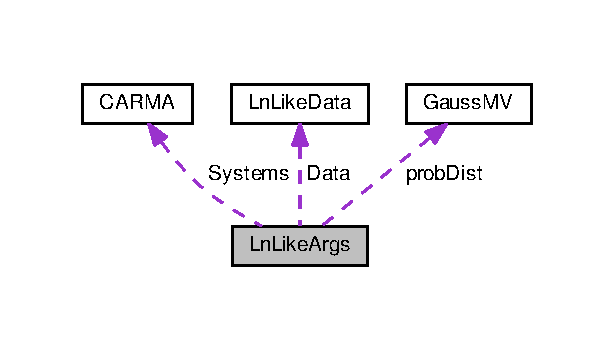
\includegraphics[width=294pt]{struct_ln_like_args__coll__graph}
\end{center}
\end{figure}
\subsection*{Public Attributes}
\begin{DoxyCompactItemize}
\item 
int \hyperlink{struct_ln_like_args_ad84da20749d9935f6a5a04b5c56d729a}{num\-Threads}
\item 
\hyperlink{class_c_a_r_m_a}{C\-A\-R\-M\-A} $\ast$ \hyperlink{struct_ln_like_args_af605bb6dcb409ad41dfc1a00c1e12c3f}{Systems}
\item 
\hyperlink{struct_ln_like_data}{Ln\-Like\-Data} \hyperlink{struct_ln_like_args_aa9a0a2c4945292f8429e4f0738db611b}{Data}
\item 
int \hyperlink{struct_ln_like_args_a14cedd7e2fed9d152ce3de6383567dad}{num\-Pts}
\item 
double $\ast$ \hyperlink{struct_ln_like_args_a49e48f13e6203cf7f629d3485416874f}{y}
\item 
\hyperlink{struct_gauss_m_v}{Gauss\-M\-V} \hyperlink{struct_ln_like_args_ad8d1ee1e21bab664c116720df98cf287}{prob\-Dist}
\end{DoxyCompactItemize}


\subsection{Detailed Description}


Definition at line 113 of file C\-A\-R\-M\-A.\-hpp.



\subsection{Member Data Documentation}
\hypertarget{struct_ln_like_args_aa9a0a2c4945292f8429e4f0738db611b}{\index{Ln\-Like\-Args@{Ln\-Like\-Args}!Data@{Data}}
\index{Data@{Data}!LnLikeArgs@{Ln\-Like\-Args}}
\subsubsection[{Data}]{\setlength{\rightskip}{0pt plus 5cm}{\bf Ln\-Like\-Data} Ln\-Like\-Args\-::\-Data}}\label{struct_ln_like_args_aa9a0a2c4945292f8429e4f0738db611b}


Definition at line 116 of file C\-A\-R\-M\-A.\-hpp.

\hypertarget{struct_ln_like_args_a14cedd7e2fed9d152ce3de6383567dad}{\index{Ln\-Like\-Args@{Ln\-Like\-Args}!num\-Pts@{num\-Pts}}
\index{num\-Pts@{num\-Pts}!LnLikeArgs@{Ln\-Like\-Args}}
\subsubsection[{num\-Pts}]{\setlength{\rightskip}{0pt plus 5cm}int Ln\-Like\-Args\-::num\-Pts}}\label{struct_ln_like_args_a14cedd7e2fed9d152ce3de6383567dad}


Definition at line 16 of file Gauss\-M\-V.\-hpp.

\hypertarget{struct_ln_like_args_ad84da20749d9935f6a5a04b5c56d729a}{\index{Ln\-Like\-Args@{Ln\-Like\-Args}!num\-Threads@{num\-Threads}}
\index{num\-Threads@{num\-Threads}!LnLikeArgs@{Ln\-Like\-Args}}
\subsubsection[{num\-Threads}]{\setlength{\rightskip}{0pt plus 5cm}int Ln\-Like\-Args\-::num\-Threads}}\label{struct_ln_like_args_ad84da20749d9935f6a5a04b5c56d729a}


Definition at line 114 of file C\-A\-R\-M\-A.\-hpp.

\hypertarget{struct_ln_like_args_ad8d1ee1e21bab664c116720df98cf287}{\index{Ln\-Like\-Args@{Ln\-Like\-Args}!prob\-Dist@{prob\-Dist}}
\index{prob\-Dist@{prob\-Dist}!LnLikeArgs@{Ln\-Like\-Args}}
\subsubsection[{prob\-Dist}]{\setlength{\rightskip}{0pt plus 5cm}{\bf Gauss\-M\-V} Ln\-Like\-Args\-::prob\-Dist}}\label{struct_ln_like_args_ad8d1ee1e21bab664c116720df98cf287}


Definition at line 18 of file Gauss\-M\-V.\-hpp.

\hypertarget{struct_ln_like_args_af605bb6dcb409ad41dfc1a00c1e12c3f}{\index{Ln\-Like\-Args@{Ln\-Like\-Args}!Systems@{Systems}}
\index{Systems@{Systems}!LnLikeArgs@{Ln\-Like\-Args}}
\subsubsection[{Systems}]{\setlength{\rightskip}{0pt plus 5cm}{\bf C\-A\-R\-M\-A}$\ast$ Ln\-Like\-Args\-::\-Systems}}\label{struct_ln_like_args_af605bb6dcb409ad41dfc1a00c1e12c3f}


Definition at line 115 of file C\-A\-R\-M\-A.\-hpp.

\hypertarget{struct_ln_like_args_a49e48f13e6203cf7f629d3485416874f}{\index{Ln\-Like\-Args@{Ln\-Like\-Args}!y@{y}}
\index{y@{y}!LnLikeArgs@{Ln\-Like\-Args}}
\subsubsection[{y}]{\setlength{\rightskip}{0pt plus 5cm}double$\ast$ Ln\-Like\-Args\-::y}}\label{struct_ln_like_args_a49e48f13e6203cf7f629d3485416874f}


Definition at line 17 of file Gauss\-M\-V.\-hpp.



The documentation for this struct was generated from the following files\-:\begin{DoxyCompactItemize}
\item 
/home/vish/code/trunk/cpp/libcarma/include/\hyperlink{_c_a_r_m_a_8hpp}{C\-A\-R\-M\-A.\-hpp}\item 
/home/vish/code/trunk/cpp/libcarma/include/\hyperlink{_gauss_m_v_8hpp}{Gauss\-M\-V.\-hpp}\end{DoxyCompactItemize}

\hypertarget{struct_ln_like_data}{\section{Ln\-Like\-Data Struct Reference}
\label{struct_ln_like_data}\index{Ln\-Like\-Data@{Ln\-Like\-Data}}
}


{\ttfamily \#include $<$C\-A\-R\-M\-A.\-hpp$>$}

\subsection*{Public Attributes}
\begin{DoxyCompactItemize}
\item 
int \hyperlink{struct_ln_like_data_a825ffbe1d96bd9f1c913ed95c83fd8de}{num\-Cadences}
\item 
bool \hyperlink{struct_ln_like_data_af49dc41383840c47d9e03c154c510912}{I\-R}
\item 
double \hyperlink{struct_ln_like_data_a0fcbb2527d414cc2b0fe576a7a61f45c}{tol\-I\-R}
\item 
double \hyperlink{struct_ln_like_data_acbb8573027fb54b1d207c126a64c49c9}{t\-\_\-incr}
\item 
double \hyperlink{struct_ln_like_data_a883ba357c5e5a7eff7fb9a25f130a0e7}{frac\-Intrinsic\-Var}
\item 
double \hyperlink{struct_ln_like_data_a9d90bcfebe1eec966719b8c0febb7dc7}{frac\-Noise\-To\-Signal}
\item 
double \hyperlink{struct_ln_like_data_ae30e91660af267721f78434f5e771293}{max\-Sigma}
\item 
double \hyperlink{struct_ln_like_data_a429a07a037a45e99a52c0c9e6193b23d}{min\-Timescale}
\item 
double \hyperlink{struct_ln_like_data_ab1c1eb4d8e84c78b1b76849adfd0aeb8}{max\-Timescale}
\item 
double $\ast$ \hyperlink{struct_ln_like_data_a5b1bf48c4b998b85df9c381974e65f93}{t}
\item 
double $\ast$ \hyperlink{struct_ln_like_data_afd71e6e5c9f90880038586d6f4e705fe}{x}
\item 
double $\ast$ \hyperlink{struct_ln_like_data_ac75cc1e68fffac23d841e09f927a0a53}{y}
\item 
double $\ast$ \hyperlink{struct_ln_like_data_a54330ef049f623a902d04f58e5aee208}{yerr}
\item 
double $\ast$ \hyperlink{struct_ln_like_data_a51c6e3bd71666d529910318735f0df21}{mask}
\end{DoxyCompactItemize}


\subsection{Detailed Description}


Definition at line 21 of file C\-A\-R\-M\-A.\-hpp.



\subsection{Member Data Documentation}
\hypertarget{struct_ln_like_data_a883ba357c5e5a7eff7fb9a25f130a0e7}{\index{Ln\-Like\-Data@{Ln\-Like\-Data}!frac\-Intrinsic\-Var@{frac\-Intrinsic\-Var}}
\index{frac\-Intrinsic\-Var@{frac\-Intrinsic\-Var}!LnLikeData@{Ln\-Like\-Data}}
\subsubsection[{frac\-Intrinsic\-Var}]{\setlength{\rightskip}{0pt plus 5cm}double Ln\-Like\-Data\-::frac\-Intrinsic\-Var}}\label{struct_ln_like_data_a883ba357c5e5a7eff7fb9a25f130a0e7}


Definition at line 26 of file C\-A\-R\-M\-A.\-hpp.

\hypertarget{struct_ln_like_data_a9d90bcfebe1eec966719b8c0febb7dc7}{\index{Ln\-Like\-Data@{Ln\-Like\-Data}!frac\-Noise\-To\-Signal@{frac\-Noise\-To\-Signal}}
\index{frac\-Noise\-To\-Signal@{frac\-Noise\-To\-Signal}!LnLikeData@{Ln\-Like\-Data}}
\subsubsection[{frac\-Noise\-To\-Signal}]{\setlength{\rightskip}{0pt plus 5cm}double Ln\-Like\-Data\-::frac\-Noise\-To\-Signal}}\label{struct_ln_like_data_a9d90bcfebe1eec966719b8c0febb7dc7}


Definition at line 27 of file C\-A\-R\-M\-A.\-hpp.

\hypertarget{struct_ln_like_data_af49dc41383840c47d9e03c154c510912}{\index{Ln\-Like\-Data@{Ln\-Like\-Data}!I\-R@{I\-R}}
\index{I\-R@{I\-R}!LnLikeData@{Ln\-Like\-Data}}
\subsubsection[{I\-R}]{\setlength{\rightskip}{0pt plus 5cm}bool Ln\-Like\-Data\-::\-I\-R}}\label{struct_ln_like_data_af49dc41383840c47d9e03c154c510912}


Definition at line 23 of file C\-A\-R\-M\-A.\-hpp.

\hypertarget{struct_ln_like_data_a51c6e3bd71666d529910318735f0df21}{\index{Ln\-Like\-Data@{Ln\-Like\-Data}!mask@{mask}}
\index{mask@{mask}!LnLikeData@{Ln\-Like\-Data}}
\subsubsection[{mask}]{\setlength{\rightskip}{0pt plus 5cm}double$\ast$ Ln\-Like\-Data\-::mask}}\label{struct_ln_like_data_a51c6e3bd71666d529910318735f0df21}


Definition at line 35 of file C\-A\-R\-M\-A.\-hpp.

\hypertarget{struct_ln_like_data_ae30e91660af267721f78434f5e771293}{\index{Ln\-Like\-Data@{Ln\-Like\-Data}!max\-Sigma@{max\-Sigma}}
\index{max\-Sigma@{max\-Sigma}!LnLikeData@{Ln\-Like\-Data}}
\subsubsection[{max\-Sigma}]{\setlength{\rightskip}{0pt plus 5cm}double Ln\-Like\-Data\-::max\-Sigma}}\label{struct_ln_like_data_ae30e91660af267721f78434f5e771293}


Definition at line 28 of file C\-A\-R\-M\-A.\-hpp.

\hypertarget{struct_ln_like_data_ab1c1eb4d8e84c78b1b76849adfd0aeb8}{\index{Ln\-Like\-Data@{Ln\-Like\-Data}!max\-Timescale@{max\-Timescale}}
\index{max\-Timescale@{max\-Timescale}!LnLikeData@{Ln\-Like\-Data}}
\subsubsection[{max\-Timescale}]{\setlength{\rightskip}{0pt plus 5cm}double Ln\-Like\-Data\-::max\-Timescale}}\label{struct_ln_like_data_ab1c1eb4d8e84c78b1b76849adfd0aeb8}


Definition at line 30 of file C\-A\-R\-M\-A.\-hpp.

\hypertarget{struct_ln_like_data_a429a07a037a45e99a52c0c9e6193b23d}{\index{Ln\-Like\-Data@{Ln\-Like\-Data}!min\-Timescale@{min\-Timescale}}
\index{min\-Timescale@{min\-Timescale}!LnLikeData@{Ln\-Like\-Data}}
\subsubsection[{min\-Timescale}]{\setlength{\rightskip}{0pt plus 5cm}double Ln\-Like\-Data\-::min\-Timescale}}\label{struct_ln_like_data_a429a07a037a45e99a52c0c9e6193b23d}


Definition at line 29 of file C\-A\-R\-M\-A.\-hpp.

\hypertarget{struct_ln_like_data_a825ffbe1d96bd9f1c913ed95c83fd8de}{\index{Ln\-Like\-Data@{Ln\-Like\-Data}!num\-Cadences@{num\-Cadences}}
\index{num\-Cadences@{num\-Cadences}!LnLikeData@{Ln\-Like\-Data}}
\subsubsection[{num\-Cadences}]{\setlength{\rightskip}{0pt plus 5cm}int Ln\-Like\-Data\-::num\-Cadences}}\label{struct_ln_like_data_a825ffbe1d96bd9f1c913ed95c83fd8de}


Definition at line 22 of file C\-A\-R\-M\-A.\-hpp.

\hypertarget{struct_ln_like_data_a5b1bf48c4b998b85df9c381974e65f93}{\index{Ln\-Like\-Data@{Ln\-Like\-Data}!t@{t}}
\index{t@{t}!LnLikeData@{Ln\-Like\-Data}}
\subsubsection[{t}]{\setlength{\rightskip}{0pt plus 5cm}double$\ast$ Ln\-Like\-Data\-::t}}\label{struct_ln_like_data_a5b1bf48c4b998b85df9c381974e65f93}


Definition at line 31 of file C\-A\-R\-M\-A.\-hpp.

\hypertarget{struct_ln_like_data_acbb8573027fb54b1d207c126a64c49c9}{\index{Ln\-Like\-Data@{Ln\-Like\-Data}!t\-\_\-incr@{t\-\_\-incr}}
\index{t\-\_\-incr@{t\-\_\-incr}!LnLikeData@{Ln\-Like\-Data}}
\subsubsection[{t\-\_\-incr}]{\setlength{\rightskip}{0pt plus 5cm}double Ln\-Like\-Data\-::t\-\_\-incr}}\label{struct_ln_like_data_acbb8573027fb54b1d207c126a64c49c9}


Definition at line 25 of file C\-A\-R\-M\-A.\-hpp.

\hypertarget{struct_ln_like_data_a0fcbb2527d414cc2b0fe576a7a61f45c}{\index{Ln\-Like\-Data@{Ln\-Like\-Data}!tol\-I\-R@{tol\-I\-R}}
\index{tol\-I\-R@{tol\-I\-R}!LnLikeData@{Ln\-Like\-Data}}
\subsubsection[{tol\-I\-R}]{\setlength{\rightskip}{0pt plus 5cm}double Ln\-Like\-Data\-::tol\-I\-R}}\label{struct_ln_like_data_a0fcbb2527d414cc2b0fe576a7a61f45c}


Definition at line 24 of file C\-A\-R\-M\-A.\-hpp.

\hypertarget{struct_ln_like_data_afd71e6e5c9f90880038586d6f4e705fe}{\index{Ln\-Like\-Data@{Ln\-Like\-Data}!x@{x}}
\index{x@{x}!LnLikeData@{Ln\-Like\-Data}}
\subsubsection[{x}]{\setlength{\rightskip}{0pt plus 5cm}double$\ast$ Ln\-Like\-Data\-::x}}\label{struct_ln_like_data_afd71e6e5c9f90880038586d6f4e705fe}


Definition at line 32 of file C\-A\-R\-M\-A.\-hpp.

\hypertarget{struct_ln_like_data_ac75cc1e68fffac23d841e09f927a0a53}{\index{Ln\-Like\-Data@{Ln\-Like\-Data}!y@{y}}
\index{y@{y}!LnLikeData@{Ln\-Like\-Data}}
\subsubsection[{y}]{\setlength{\rightskip}{0pt plus 5cm}double$\ast$ Ln\-Like\-Data\-::y}}\label{struct_ln_like_data_ac75cc1e68fffac23d841e09f927a0a53}


Definition at line 33 of file C\-A\-R\-M\-A.\-hpp.

\hypertarget{struct_ln_like_data_a54330ef049f623a902d04f58e5aee208}{\index{Ln\-Like\-Data@{Ln\-Like\-Data}!yerr@{yerr}}
\index{yerr@{yerr}!LnLikeData@{Ln\-Like\-Data}}
\subsubsection[{yerr}]{\setlength{\rightskip}{0pt plus 5cm}double$\ast$ Ln\-Like\-Data\-::yerr}}\label{struct_ln_like_data_a54330ef049f623a902d04f58e5aee208}


Definition at line 34 of file C\-A\-R\-M\-A.\-hpp.



The documentation for this struct was generated from the following file\-:\begin{DoxyCompactItemize}
\item 
/home/vish/code/trunk/cpp/libcarma/cython/include/\hyperlink{_c_a_r_m_a_8hpp}{C\-A\-R\-M\-A.\-hpp}\end{DoxyCompactItemize}

\hypertarget{classpython_1_1libcarma_1_1libcarma_1_1task}{\section{python.\-libcarma.\-libcarma.\-task Class Reference}
\label{classpython_1_1libcarma_1_1libcarma_1_1task}\index{python.\-libcarma.\-libcarma.\-task@{python.\-libcarma.\-libcarma.\-task}}
}


Inheritance diagram for python.\-libcarma.\-libcarma.\-task\-:


Collaboration diagram for python.\-libcarma.\-libcarma.\-task\-:
\subsection*{Public Member Functions}
\begin{DoxyCompactItemize}
\item 
def \hyperlink{classpython_1_1libcarma_1_1libcarma_1_1task_a56a77b3fb1dc1cfc7755f3a393351ce6}{\-\_\-\-\_\-init\-\_\-\-\_\-}
\item 
def \hyperlink{classpython_1_1libcarma_1_1libcarma_1_1task_a94744fa39163415ffcaf0d62d40fca0a}{p}
\item 
def \hyperlink{classpython_1_1libcarma_1_1libcarma_1_1task_a94744fa39163415ffcaf0d62d40fca0a}{p}
\item 
def \hyperlink{classpython_1_1libcarma_1_1libcarma_1_1task_aa81a6ec3a0273a08b157673c847dbfd7}{q}
\item 
def \hyperlink{classpython_1_1libcarma_1_1libcarma_1_1task_aa81a6ec3a0273a08b157673c847dbfd7}{q}
\item 
def \hyperlink{classpython_1_1libcarma_1_1libcarma_1_1task_a6e635f95fe65a97b184579c9f541ddd5}{nthreads}
\item 
def \hyperlink{classpython_1_1libcarma_1_1libcarma_1_1task_a5583472b31550f268e3290ec4c3ad7af}{nburn}
\item 
def \hyperlink{classpython_1_1libcarma_1_1libcarma_1_1task_a5583472b31550f268e3290ec4c3ad7af}{nburn}
\item 
def \hyperlink{classpython_1_1libcarma_1_1libcarma_1_1task_a136998a257bc82c4df663d46871a7f51}{nwalkers}
\item 
def \hyperlink{classpython_1_1libcarma_1_1libcarma_1_1task_a136998a257bc82c4df663d46871a7f51}{nwalkers}
\item 
def \hyperlink{classpython_1_1libcarma_1_1libcarma_1_1task_af6f36241731b24af9e6872106f2d6eab}{nsteps}
\item 
def \hyperlink{classpython_1_1libcarma_1_1libcarma_1_1task_af6f36241731b24af9e6872106f2d6eab}{nsteps}
\item 
def \hyperlink{classpython_1_1libcarma_1_1libcarma_1_1task_a93494b990ffb8ca498b6d0d6512a7fa7}{scatter\-Factor}
\item 
def \hyperlink{classpython_1_1libcarma_1_1libcarma_1_1task_a93494b990ffb8ca498b6d0d6512a7fa7}{scatter\-Factor}
\item 
def \hyperlink{classpython_1_1libcarma_1_1libcarma_1_1task_a54458b7bfc6f1daa4619b3c11709bc28}{max\-Evals}
\item 
def \hyperlink{classpython_1_1libcarma_1_1libcarma_1_1task_a54458b7bfc6f1daa4619b3c11709bc28}{max\-Evals}
\item 
def \hyperlink{classpython_1_1libcarma_1_1libcarma_1_1task_ad09f62c696166c2910061f4c7558d5cd}{x\-Tol}
\item 
def \hyperlink{classpython_1_1libcarma_1_1libcarma_1_1task_ad09f62c696166c2910061f4c7558d5cd}{x\-Tol}
\item 
def \hyperlink{classpython_1_1libcarma_1_1libcarma_1_1task_aa3738370648b6c61609a82e58d5456f5}{Chain}
\item 
def \hyperlink{classpython_1_1libcarma_1_1libcarma_1_1task_a2d8d395adefebba18b97872971d14ec0}{Ln\-Posterior}
\item 
def \hyperlink{classpython_1_1libcarma_1_1libcarma_1_1task_a1e50e377e383eb8d28884f7dc8fb095e}{\-\_\-\-\_\-repr\-\_\-\-\_\-}
\item 
def \hyperlink{classpython_1_1libcarma_1_1libcarma_1_1task_a16f2cab7a7b342a747c96850329b6983}{\-\_\-\-\_\-str\-\_\-\-\_\-}
\item 
def \hyperlink{classpython_1_1libcarma_1_1libcarma_1_1task_af41200b3fedc615736fa2efdc0e9fead}{\-\_\-\-\_\-eq\-\_\-\-\_\-}
\item 
def \hyperlink{classpython_1_1libcarma_1_1libcarma_1_1task_a5010d0e3ed86802c91685363ef2593df}{\-\_\-\-\_\-neq\-\_\-\-\_\-}
\item 
def \hyperlink{classpython_1_1libcarma_1_1libcarma_1_1task_a60148b65c4e79bd848695d837b9bf5a5}{reset}
\item 
def \hyperlink{classpython_1_1libcarma_1_1libcarma_1_1task_a58ea30a7a53358667aab9e9c245a8b0e}{check}
\item 
def \hyperlink{classpython_1_1libcarma_1_1libcarma_1_1task_af0e7f38c6e6f539a3c278123caaca0d5}{set}
\item 
def \hyperlink{classpython_1_1libcarma_1_1libcarma_1_1task_af21382fcabf13ecdbd3837509ab82f3d}{dt}
\item 
def \hyperlink{classpython_1_1libcarma_1_1libcarma_1_1task_ae5b13aeb5d099d38cb77a53b3a5f88d0}{Theta}
\item 
def \hyperlink{classpython_1_1libcarma_1_1libcarma_1_1task_a036a7f2657ec716f9302f9cc5d15449d}{list}
\item 
def \hyperlink{classpython_1_1libcarma_1_1libcarma_1_1task_a9b3a40d7904e96ba27cf91e286cfa599}{show}
\item 
def \hyperlink{classpython_1_1libcarma_1_1libcarma_1_1task_a055e8ca28b2115ec7a8434a68a4f812b}{Sigma}
\item 
def \hyperlink{classpython_1_1libcarma_1_1libcarma_1_1task_ac6b18e34b346ea7ad41c030de9c53f69}{simulate}
\item 
def \hyperlink{classpython_1_1libcarma_1_1libcarma_1_1task_a3e8b381e5920139ac7ae60406792f4f2}{observe}
\item 
def \hyperlink{classpython_1_1libcarma_1_1libcarma_1_1task_a8f9c2672ecb99eba7937d0cab3878c76}{log\-Prior}
\item 
def \hyperlink{classpython_1_1libcarma_1_1libcarma_1_1task_aee49abd18b0a2beea70eba28352edd8d}{log\-Likelihood}
\item 
def \hyperlink{classpython_1_1libcarma_1_1libcarma_1_1task_a4f0a4fa5a145400b19ac43b981e005b7}{log\-Posterior}
\item 
def \hyperlink{classpython_1_1libcarma_1_1libcarma_1_1task_a41483bb32afa386c3b39fd99b5e158e5}{fit}
\end{DoxyCompactItemize}
\subsection*{Public Attributes}
\begin{DoxyCompactItemize}
\item 
\hyperlink{classpython_1_1libcarma_1_1libcarma_1_1task_a6d4e69f1f43143928d306660a0ad78c1}{x\-Tol}
\end{DoxyCompactItemize}


\subsection{Detailed Description}


Definition at line 286 of file libcarma.\-py.



\subsection{Constructor \& Destructor Documentation}
\hypertarget{classpython_1_1libcarma_1_1libcarma_1_1task_a56a77b3fb1dc1cfc7755f3a393351ce6}{\index{python\-::libcarma\-::libcarma\-::task@{python\-::libcarma\-::libcarma\-::task}!\-\_\-\-\_\-init\-\_\-\-\_\-@{\-\_\-\-\_\-init\-\_\-\-\_\-}}
\index{\-\_\-\-\_\-init\-\_\-\-\_\-@{\-\_\-\-\_\-init\-\_\-\-\_\-}!python::libcarma::libcarma::task@{python\-::libcarma\-::libcarma\-::task}}
\subsubsection[{\-\_\-\-\_\-init\-\_\-\-\_\-}]{\setlength{\rightskip}{0pt plus 5cm}def python.\-libcarma.\-libcarma.\-task.\-\_\-\-\_\-init\-\_\-\-\_\- (
\begin{DoxyParamCaption}
\item[{}]{self, }
\item[{}]{p, }
\item[{}]{q, }
\item[{}]{nthreads = {\ttfamily psutil.cpu\-\_\-count(logical~=~False)}, }
\item[{}]{nburn = {\ttfamily 1000000}, }
\item[{}]{nwalkers = {\ttfamily 25$\ast$psutil.cpu\-\_\-count(logical~=~False)}, }
\item[{}]{nsteps = {\ttfamily 250}, }
\item[{}]{scatter\-Factor = {\ttfamily 1.0e-\/1}, }
\item[{}]{max\-Evals = {\ttfamily 1000}, }
\item[{}]{x\-Tol = {\ttfamily 0.005}}
\end{DoxyParamCaption}
)}}\label{classpython_1_1libcarma_1_1libcarma_1_1task_a56a77b3fb1dc1cfc7755f3a393351ce6}


Definition at line 288 of file libcarma.\-py.



\subsection{Member Function Documentation}
\hypertarget{classpython_1_1libcarma_1_1libcarma_1_1task_af41200b3fedc615736fa2efdc0e9fead}{\index{python\-::libcarma\-::libcarma\-::task@{python\-::libcarma\-::libcarma\-::task}!\-\_\-\-\_\-eq\-\_\-\-\_\-@{\-\_\-\-\_\-eq\-\_\-\-\_\-}}
\index{\-\_\-\-\_\-eq\-\_\-\-\_\-@{\-\_\-\-\_\-eq\-\_\-\-\_\-}!python::libcarma::libcarma::task@{python\-::libcarma\-::libcarma\-::task}}
\subsubsection[{\-\_\-\-\_\-eq\-\_\-\-\_\-}]{\setlength{\rightskip}{0pt plus 5cm}def python.\-libcarma.\-libcarma.\-task.\-\_\-\-\_\-eq\-\_\-\-\_\- (
\begin{DoxyParamCaption}
\item[{}]{self, }
\item[{}]{other}
\end{DoxyParamCaption}
)}}\label{classpython_1_1libcarma_1_1libcarma_1_1task_af41200b3fedc615736fa2efdc0e9fead}


Definition at line 468 of file libcarma.\-py.

\hypertarget{classpython_1_1libcarma_1_1libcarma_1_1task_a5010d0e3ed86802c91685363ef2593df}{\index{python\-::libcarma\-::libcarma\-::task@{python\-::libcarma\-::libcarma\-::task}!\-\_\-\-\_\-neq\-\_\-\-\_\-@{\-\_\-\-\_\-neq\-\_\-\-\_\-}}
\index{\-\_\-\-\_\-neq\-\_\-\-\_\-@{\-\_\-\-\_\-neq\-\_\-\-\_\-}!python::libcarma::libcarma::task@{python\-::libcarma\-::libcarma\-::task}}
\subsubsection[{\-\_\-\-\_\-neq\-\_\-\-\_\-}]{\setlength{\rightskip}{0pt plus 5cm}def python.\-libcarma.\-libcarma.\-task.\-\_\-\-\_\-neq\-\_\-\-\_\- (
\begin{DoxyParamCaption}
\item[{}]{self, }
\item[{}]{other}
\end{DoxyParamCaption}
)}}\label{classpython_1_1libcarma_1_1libcarma_1_1task_a5010d0e3ed86802c91685363ef2593df}


Definition at line 477 of file libcarma.\-py.

\hypertarget{classpython_1_1libcarma_1_1libcarma_1_1task_a1e50e377e383eb8d28884f7dc8fb095e}{\index{python\-::libcarma\-::libcarma\-::task@{python\-::libcarma\-::libcarma\-::task}!\-\_\-\-\_\-repr\-\_\-\-\_\-@{\-\_\-\-\_\-repr\-\_\-\-\_\-}}
\index{\-\_\-\-\_\-repr\-\_\-\-\_\-@{\-\_\-\-\_\-repr\-\_\-\-\_\-}!python::libcarma::libcarma::task@{python\-::libcarma\-::libcarma\-::task}}
\subsubsection[{\-\_\-\-\_\-repr\-\_\-\-\_\-}]{\setlength{\rightskip}{0pt plus 5cm}def python.\-libcarma.\-libcarma.\-task.\-\_\-\-\_\-repr\-\_\-\-\_\- (
\begin{DoxyParamCaption}
\item[{}]{self}
\end{DoxyParamCaption}
)}}\label{classpython_1_1libcarma_1_1libcarma_1_1task_a1e50e377e383eb8d28884f7dc8fb095e}


Definition at line 454 of file libcarma.\-py.

\hypertarget{classpython_1_1libcarma_1_1libcarma_1_1task_a16f2cab7a7b342a747c96850329b6983}{\index{python\-::libcarma\-::libcarma\-::task@{python\-::libcarma\-::libcarma\-::task}!\-\_\-\-\_\-str\-\_\-\-\_\-@{\-\_\-\-\_\-str\-\_\-\-\_\-}}
\index{\-\_\-\-\_\-str\-\_\-\-\_\-@{\-\_\-\-\_\-str\-\_\-\-\_\-}!python::libcarma::libcarma::task@{python\-::libcarma\-::libcarma\-::task}}
\subsubsection[{\-\_\-\-\_\-str\-\_\-\-\_\-}]{\setlength{\rightskip}{0pt plus 5cm}def python.\-libcarma.\-libcarma.\-task.\-\_\-\-\_\-str\-\_\-\-\_\- (
\begin{DoxyParamCaption}
\item[{}]{self}
\end{DoxyParamCaption}
)}}\label{classpython_1_1libcarma_1_1libcarma_1_1task_a16f2cab7a7b342a747c96850329b6983}


Definition at line 457 of file libcarma.\-py.



Here is the call graph for this function\-:


\hypertarget{classpython_1_1libcarma_1_1libcarma_1_1task_aa3738370648b6c61609a82e58d5456f5}{\index{python\-::libcarma\-::libcarma\-::task@{python\-::libcarma\-::libcarma\-::task}!Chain@{Chain}}
\index{Chain@{Chain}!python::libcarma::libcarma::task@{python\-::libcarma\-::libcarma\-::task}}
\subsubsection[{Chain}]{\setlength{\rightskip}{0pt plus 5cm}def python.\-libcarma.\-libcarma.\-task.\-Chain (
\begin{DoxyParamCaption}
\item[{}]{self}
\end{DoxyParamCaption}
)}}\label{classpython_1_1libcarma_1_1libcarma_1_1task_aa3738370648b6c61609a82e58d5456f5}


Definition at line 447 of file libcarma.\-py.

\hypertarget{classpython_1_1libcarma_1_1libcarma_1_1task_a58ea30a7a53358667aab9e9c245a8b0e}{\index{python\-::libcarma\-::libcarma\-::task@{python\-::libcarma\-::libcarma\-::task}!check@{check}}
\index{check@{check}!python::libcarma::libcarma::task@{python\-::libcarma\-::libcarma\-::task}}
\subsubsection[{check}]{\setlength{\rightskip}{0pt plus 5cm}def python.\-libcarma.\-libcarma.\-task.\-check (
\begin{DoxyParamCaption}
\item[{}]{self, }
\item[{}]{Theta, }
\item[{}]{tnum = {\ttfamily None}}
\end{DoxyParamCaption}
)}}\label{classpython_1_1libcarma_1_1libcarma_1_1task_a58ea30a7a53358667aab9e9c245a8b0e}


Definition at line 518 of file libcarma.\-py.

\hypertarget{classpython_1_1libcarma_1_1libcarma_1_1task_af21382fcabf13ecdbd3837509ab82f3d}{\index{python\-::libcarma\-::libcarma\-::task@{python\-::libcarma\-::libcarma\-::task}!dt@{dt}}
\index{dt@{dt}!python::libcarma::libcarma::task@{python\-::libcarma\-::libcarma\-::task}}
\subsubsection[{dt}]{\setlength{\rightskip}{0pt plus 5cm}def python.\-libcarma.\-libcarma.\-task.\-dt (
\begin{DoxyParamCaption}
\item[{}]{self, }
\item[{}]{tnum = {\ttfamily None}}
\end{DoxyParamCaption}
)}}\label{classpython_1_1libcarma_1_1libcarma_1_1task_af21382fcabf13ecdbd3837509ab82f3d}


Definition at line 532 of file libcarma.\-py.

\hypertarget{classpython_1_1libcarma_1_1libcarma_1_1task_a41483bb32afa386c3b39fd99b5e158e5}{\index{python\-::libcarma\-::libcarma\-::task@{python\-::libcarma\-::libcarma\-::task}!fit@{fit}}
\index{fit@{fit}!python::libcarma::libcarma::task@{python\-::libcarma\-::libcarma\-::task}}
\subsubsection[{fit}]{\setlength{\rightskip}{0pt plus 5cm}def python.\-libcarma.\-libcarma.\-task.\-fit (
\begin{DoxyParamCaption}
\item[{}]{self, }
\item[{}]{observed\-L\-C, }
\item[{}]{x\-Start, }
\item[{}]{z\-S\-Seed = {\ttfamily None}, }
\item[{}]{walker\-Seed = {\ttfamily None}, }
\item[{}]{move\-Seed = {\ttfamily None}, }
\item[{}]{x\-Seed = {\ttfamily None}}
\end{DoxyParamCaption}
)}}\label{classpython_1_1libcarma_1_1libcarma_1_1task_a41483bb32afa386c3b39fd99b5e158e5}


Definition at line 618 of file libcarma.\-py.



Here is the call graph for this function\-:


\hypertarget{classpython_1_1libcarma_1_1libcarma_1_1task_a036a7f2657ec716f9302f9cc5d15449d}{\index{python\-::libcarma\-::libcarma\-::task@{python\-::libcarma\-::libcarma\-::task}!list@{list}}
\index{list@{list}!python::libcarma::libcarma::task@{python\-::libcarma\-::libcarma\-::task}}
\subsubsection[{list}]{\setlength{\rightskip}{0pt plus 5cm}def python.\-libcarma.\-libcarma.\-task.\-list (
\begin{DoxyParamCaption}
\item[{}]{self}
\end{DoxyParamCaption}
)}}\label{classpython_1_1libcarma_1_1libcarma_1_1task_a036a7f2657ec716f9302f9cc5d15449d}


Definition at line 544 of file libcarma.\-py.

\hypertarget{classpython_1_1libcarma_1_1libcarma_1_1task_a2d8d395adefebba18b97872971d14ec0}{\index{python\-::libcarma\-::libcarma\-::task@{python\-::libcarma\-::libcarma\-::task}!Ln\-Posterior@{Ln\-Posterior}}
\index{Ln\-Posterior@{Ln\-Posterior}!python::libcarma::libcarma::task@{python\-::libcarma\-::libcarma\-::task}}
\subsubsection[{Ln\-Posterior}]{\setlength{\rightskip}{0pt plus 5cm}def python.\-libcarma.\-libcarma.\-task.\-Ln\-Posterior (
\begin{DoxyParamCaption}
\item[{}]{self}
\end{DoxyParamCaption}
)}}\label{classpython_1_1libcarma_1_1libcarma_1_1task_a2d8d395adefebba18b97872971d14ec0}


Definition at line 451 of file libcarma.\-py.

\hypertarget{classpython_1_1libcarma_1_1libcarma_1_1task_aee49abd18b0a2beea70eba28352edd8d}{\index{python\-::libcarma\-::libcarma\-::task@{python\-::libcarma\-::libcarma\-::task}!log\-Likelihood@{log\-Likelihood}}
\index{log\-Likelihood@{log\-Likelihood}!python::libcarma::libcarma::task@{python\-::libcarma\-::libcarma\-::task}}
\subsubsection[{log\-Likelihood}]{\setlength{\rightskip}{0pt plus 5cm}def python.\-libcarma.\-libcarma.\-task.\-log\-Likelihood (
\begin{DoxyParamCaption}
\item[{}]{self, }
\item[{}]{observed\-L\-C, }
\item[{}]{tnum = {\ttfamily None}}
\end{DoxyParamCaption}
)}}\label{classpython_1_1libcarma_1_1libcarma_1_1task_aee49abd18b0a2beea70eba28352edd8d}


Definition at line 608 of file libcarma.\-py.

\hypertarget{classpython_1_1libcarma_1_1libcarma_1_1task_a4f0a4fa5a145400b19ac43b981e005b7}{\index{python\-::libcarma\-::libcarma\-::task@{python\-::libcarma\-::libcarma\-::task}!log\-Posterior@{log\-Posterior}}
\index{log\-Posterior@{log\-Posterior}!python::libcarma::libcarma::task@{python\-::libcarma\-::libcarma\-::task}}
\subsubsection[{log\-Posterior}]{\setlength{\rightskip}{0pt plus 5cm}def python.\-libcarma.\-libcarma.\-task.\-log\-Posterior (
\begin{DoxyParamCaption}
\item[{}]{self, }
\item[{}]{observed\-L\-C, }
\item[{}]{tnum = {\ttfamily None}}
\end{DoxyParamCaption}
)}}\label{classpython_1_1libcarma_1_1libcarma_1_1task_a4f0a4fa5a145400b19ac43b981e005b7}


Definition at line 613 of file libcarma.\-py.

\hypertarget{classpython_1_1libcarma_1_1libcarma_1_1task_a8f9c2672ecb99eba7937d0cab3878c76}{\index{python\-::libcarma\-::libcarma\-::task@{python\-::libcarma\-::libcarma\-::task}!log\-Prior@{log\-Prior}}
\index{log\-Prior@{log\-Prior}!python::libcarma::libcarma::task@{python\-::libcarma\-::libcarma\-::task}}
\subsubsection[{log\-Prior}]{\setlength{\rightskip}{0pt plus 5cm}def python.\-libcarma.\-libcarma.\-task.\-log\-Prior (
\begin{DoxyParamCaption}
\item[{}]{self, }
\item[{}]{observed\-L\-C, }
\item[{}]{tnum = {\ttfamily None}}
\end{DoxyParamCaption}
)}}\label{classpython_1_1libcarma_1_1libcarma_1_1task_a8f9c2672ecb99eba7937d0cab3878c76}


Definition at line 603 of file libcarma.\-py.

\hypertarget{classpython_1_1libcarma_1_1libcarma_1_1task_a54458b7bfc6f1daa4619b3c11709bc28}{\index{python\-::libcarma\-::libcarma\-::task@{python\-::libcarma\-::libcarma\-::task}!max\-Evals@{max\-Evals}}
\index{max\-Evals@{max\-Evals}!python::libcarma::libcarma::task@{python\-::libcarma\-::libcarma\-::task}}
\subsubsection[{max\-Evals}]{\setlength{\rightskip}{0pt plus 5cm}def python.\-libcarma.\-libcarma.\-task.\-max\-Evals (
\begin{DoxyParamCaption}
\item[{}]{self}
\end{DoxyParamCaption}
)}}\label{classpython_1_1libcarma_1_1libcarma_1_1task_a54458b7bfc6f1daa4619b3c11709bc28}


Definition at line 421 of file libcarma.\-py.



Here is the caller graph for this function\-:


\hypertarget{classpython_1_1libcarma_1_1libcarma_1_1task_a54458b7bfc6f1daa4619b3c11709bc28}{\index{python\-::libcarma\-::libcarma\-::task@{python\-::libcarma\-::libcarma\-::task}!max\-Evals@{max\-Evals}}
\index{max\-Evals@{max\-Evals}!python::libcarma::libcarma::task@{python\-::libcarma\-::libcarma\-::task}}
\subsubsection[{max\-Evals}]{\setlength{\rightskip}{0pt plus 5cm}def python.\-libcarma.\-libcarma.\-task.\-max\-Evals (
\begin{DoxyParamCaption}
\item[{}]{self, }
\item[{}]{value}
\end{DoxyParamCaption}
)}}\label{classpython_1_1libcarma_1_1libcarma_1_1task_a54458b7bfc6f1daa4619b3c11709bc28}


Definition at line 425 of file libcarma.\-py.



Here is the call graph for this function\-:


\hypertarget{classpython_1_1libcarma_1_1libcarma_1_1task_a5583472b31550f268e3290ec4c3ad7af}{\index{python\-::libcarma\-::libcarma\-::task@{python\-::libcarma\-::libcarma\-::task}!nburn@{nburn}}
\index{nburn@{nburn}!python::libcarma::libcarma::task@{python\-::libcarma\-::libcarma\-::task}}
\subsubsection[{nburn}]{\setlength{\rightskip}{0pt plus 5cm}def python.\-libcarma.\-libcarma.\-task.\-nburn (
\begin{DoxyParamCaption}
\item[{}]{self}
\end{DoxyParamCaption}
)}}\label{classpython_1_1libcarma_1_1libcarma_1_1task_a5583472b31550f268e3290ec4c3ad7af}


Definition at line 364 of file libcarma.\-py.



Here is the caller graph for this function\-:


\hypertarget{classpython_1_1libcarma_1_1libcarma_1_1task_a5583472b31550f268e3290ec4c3ad7af}{\index{python\-::libcarma\-::libcarma\-::task@{python\-::libcarma\-::libcarma\-::task}!nburn@{nburn}}
\index{nburn@{nburn}!python::libcarma::libcarma::task@{python\-::libcarma\-::libcarma\-::task}}
\subsubsection[{nburn}]{\setlength{\rightskip}{0pt plus 5cm}def python.\-libcarma.\-libcarma.\-task.\-nburn (
\begin{DoxyParamCaption}
\item[{}]{self, }
\item[{}]{nburn\-Val}
\end{DoxyParamCaption}
)}}\label{classpython_1_1libcarma_1_1libcarma_1_1task_a5583472b31550f268e3290ec4c3ad7af}


Definition at line 368 of file libcarma.\-py.



Here is the call graph for this function\-:


\hypertarget{classpython_1_1libcarma_1_1libcarma_1_1task_af6f36241731b24af9e6872106f2d6eab}{\index{python\-::libcarma\-::libcarma\-::task@{python\-::libcarma\-::libcarma\-::task}!nsteps@{nsteps}}
\index{nsteps@{nsteps}!python::libcarma::libcarma::task@{python\-::libcarma\-::libcarma\-::task}}
\subsubsection[{nsteps}]{\setlength{\rightskip}{0pt plus 5cm}def python.\-libcarma.\-libcarma.\-task.\-nsteps (
\begin{DoxyParamCaption}
\item[{}]{self}
\end{DoxyParamCaption}
)}}\label{classpython_1_1libcarma_1_1libcarma_1_1task_af6f36241731b24af9e6872106f2d6eab}


Definition at line 393 of file libcarma.\-py.



Here is the caller graph for this function\-:


\hypertarget{classpython_1_1libcarma_1_1libcarma_1_1task_af6f36241731b24af9e6872106f2d6eab}{\index{python\-::libcarma\-::libcarma\-::task@{python\-::libcarma\-::libcarma\-::task}!nsteps@{nsteps}}
\index{nsteps@{nsteps}!python::libcarma::libcarma::task@{python\-::libcarma\-::libcarma\-::task}}
\subsubsection[{nsteps}]{\setlength{\rightskip}{0pt plus 5cm}def python.\-libcarma.\-libcarma.\-task.\-nsteps (
\begin{DoxyParamCaption}
\item[{}]{self, }
\item[{}]{value}
\end{DoxyParamCaption}
)}}\label{classpython_1_1libcarma_1_1libcarma_1_1task_af6f36241731b24af9e6872106f2d6eab}


Definition at line 397 of file libcarma.\-py.



Here is the call graph for this function\-:


\hypertarget{classpython_1_1libcarma_1_1libcarma_1_1task_a6e635f95fe65a97b184579c9f541ddd5}{\index{python\-::libcarma\-::libcarma\-::task@{python\-::libcarma\-::libcarma\-::task}!nthreads@{nthreads}}
\index{nthreads@{nthreads}!python::libcarma::libcarma::task@{python\-::libcarma\-::libcarma\-::task}}
\subsubsection[{nthreads}]{\setlength{\rightskip}{0pt plus 5cm}def python.\-libcarma.\-libcarma.\-task.\-nthreads (
\begin{DoxyParamCaption}
\item[{}]{self}
\end{DoxyParamCaption}
)}}\label{classpython_1_1libcarma_1_1libcarma_1_1task_a6e635f95fe65a97b184579c9f541ddd5}


Definition at line 360 of file libcarma.\-py.

\hypertarget{classpython_1_1libcarma_1_1libcarma_1_1task_a136998a257bc82c4df663d46871a7f51}{\index{python\-::libcarma\-::libcarma\-::task@{python\-::libcarma\-::libcarma\-::task}!nwalkers@{nwalkers}}
\index{nwalkers@{nwalkers}!python::libcarma::libcarma::task@{python\-::libcarma\-::libcarma\-::task}}
\subsubsection[{nwalkers}]{\setlength{\rightskip}{0pt plus 5cm}def python.\-libcarma.\-libcarma.\-task.\-nwalkers (
\begin{DoxyParamCaption}
\item[{}]{self}
\end{DoxyParamCaption}
)}}\label{classpython_1_1libcarma_1_1libcarma_1_1task_a136998a257bc82c4df663d46871a7f51}


Definition at line 378 of file libcarma.\-py.



Here is the caller graph for this function\-:


\hypertarget{classpython_1_1libcarma_1_1libcarma_1_1task_a136998a257bc82c4df663d46871a7f51}{\index{python\-::libcarma\-::libcarma\-::task@{python\-::libcarma\-::libcarma\-::task}!nwalkers@{nwalkers}}
\index{nwalkers@{nwalkers}!python::libcarma::libcarma::task@{python\-::libcarma\-::libcarma\-::task}}
\subsubsection[{nwalkers}]{\setlength{\rightskip}{0pt plus 5cm}def python.\-libcarma.\-libcarma.\-task.\-nwalkers (
\begin{DoxyParamCaption}
\item[{}]{self, }
\item[{}]{value}
\end{DoxyParamCaption}
)}}\label{classpython_1_1libcarma_1_1libcarma_1_1task_a136998a257bc82c4df663d46871a7f51}


Definition at line 382 of file libcarma.\-py.



Here is the call graph for this function\-:


\hypertarget{classpython_1_1libcarma_1_1libcarma_1_1task_a3e8b381e5920139ac7ae60406792f4f2}{\index{python\-::libcarma\-::libcarma\-::task@{python\-::libcarma\-::libcarma\-::task}!observe@{observe}}
\index{observe@{observe}!python::libcarma::libcarma::task@{python\-::libcarma\-::libcarma\-::task}}
\subsubsection[{observe}]{\setlength{\rightskip}{0pt plus 5cm}def python.\-libcarma.\-libcarma.\-task.\-observe (
\begin{DoxyParamCaption}
\item[{}]{self, }
\item[{}]{intrinsic\-L\-C, }
\item[{}]{noise\-Seed = {\ttfamily None}, }
\item[{}]{tnum = {\ttfamily None}}
\end{DoxyParamCaption}
)}}\label{classpython_1_1libcarma_1_1libcarma_1_1task_a3e8b381e5920139ac7ae60406792f4f2}


Definition at line 592 of file libcarma.\-py.

\hypertarget{classpython_1_1libcarma_1_1libcarma_1_1task_a94744fa39163415ffcaf0d62d40fca0a}{\index{python\-::libcarma\-::libcarma\-::task@{python\-::libcarma\-::libcarma\-::task}!p@{p}}
\index{p@{p}!python::libcarma::libcarma::task@{python\-::libcarma\-::libcarma\-::task}}
\subsubsection[{p}]{\setlength{\rightskip}{0pt plus 5cm}def python.\-libcarma.\-libcarma.\-task.\-p (
\begin{DoxyParamCaption}
\item[{}]{self}
\end{DoxyParamCaption}
)}}\label{classpython_1_1libcarma_1_1libcarma_1_1task_a94744fa39163415ffcaf0d62d40fca0a}


Definition at line 326 of file libcarma.\-py.



Here is the caller graph for this function\-:


\hypertarget{classpython_1_1libcarma_1_1libcarma_1_1task_a94744fa39163415ffcaf0d62d40fca0a}{\index{python\-::libcarma\-::libcarma\-::task@{python\-::libcarma\-::libcarma\-::task}!p@{p}}
\index{p@{p}!python::libcarma::libcarma::task@{python\-::libcarma\-::libcarma\-::task}}
\subsubsection[{p}]{\setlength{\rightskip}{0pt plus 5cm}def python.\-libcarma.\-libcarma.\-task.\-p (
\begin{DoxyParamCaption}
\item[{}]{self, }
\item[{}]{value}
\end{DoxyParamCaption}
)}}\label{classpython_1_1libcarma_1_1libcarma_1_1task_a94744fa39163415ffcaf0d62d40fca0a}


Definition at line 330 of file libcarma.\-py.



Here is the call graph for this function\-:


\hypertarget{classpython_1_1libcarma_1_1libcarma_1_1task_aa81a6ec3a0273a08b157673c847dbfd7}{\index{python\-::libcarma\-::libcarma\-::task@{python\-::libcarma\-::libcarma\-::task}!q@{q}}
\index{q@{q}!python::libcarma::libcarma::task@{python\-::libcarma\-::libcarma\-::task}}
\subsubsection[{q}]{\setlength{\rightskip}{0pt plus 5cm}def python.\-libcarma.\-libcarma.\-task.\-q (
\begin{DoxyParamCaption}
\item[{}]{self}
\end{DoxyParamCaption}
)}}\label{classpython_1_1libcarma_1_1libcarma_1_1task_aa81a6ec3a0273a08b157673c847dbfd7}


Definition at line 343 of file libcarma.\-py.



Here is the caller graph for this function\-:


\hypertarget{classpython_1_1libcarma_1_1libcarma_1_1task_aa81a6ec3a0273a08b157673c847dbfd7}{\index{python\-::libcarma\-::libcarma\-::task@{python\-::libcarma\-::libcarma\-::task}!q@{q}}
\index{q@{q}!python::libcarma::libcarma::task@{python\-::libcarma\-::libcarma\-::task}}
\subsubsection[{q}]{\setlength{\rightskip}{0pt plus 5cm}def python.\-libcarma.\-libcarma.\-task.\-q (
\begin{DoxyParamCaption}
\item[{}]{self, }
\item[{}]{value}
\end{DoxyParamCaption}
)}}\label{classpython_1_1libcarma_1_1libcarma_1_1task_aa81a6ec3a0273a08b157673c847dbfd7}


Definition at line 347 of file libcarma.\-py.



Here is the call graph for this function\-:


\hypertarget{classpython_1_1libcarma_1_1libcarma_1_1task_a60148b65c4e79bd848695d837b9bf5a5}{\index{python\-::libcarma\-::libcarma\-::task@{python\-::libcarma\-::libcarma\-::task}!reset@{reset}}
\index{reset@{reset}!python::libcarma::libcarma::task@{python\-::libcarma\-::libcarma\-::task}}
\subsubsection[{reset}]{\setlength{\rightskip}{0pt plus 5cm}def python.\-libcarma.\-libcarma.\-task.\-reset (
\begin{DoxyParamCaption}
\item[{}]{self, }
\item[{}]{p = {\ttfamily None}, }
\item[{}]{q = {\ttfamily None}, }
\item[{}]{nburn = {\ttfamily None}, }
\item[{}]{nwalkers = {\ttfamily None}, }
\item[{}]{nsteps = {\ttfamily None}}
\end{DoxyParamCaption}
)}}\label{classpython_1_1libcarma_1_1libcarma_1_1task_a60148b65c4e79bd848695d837b9bf5a5}


Definition at line 483 of file libcarma.\-py.

\hypertarget{classpython_1_1libcarma_1_1libcarma_1_1task_a93494b990ffb8ca498b6d0d6512a7fa7}{\index{python\-::libcarma\-::libcarma\-::task@{python\-::libcarma\-::libcarma\-::task}!scatter\-Factor@{scatter\-Factor}}
\index{scatter\-Factor@{scatter\-Factor}!python::libcarma::libcarma::task@{python\-::libcarma\-::libcarma\-::task}}
\subsubsection[{scatter\-Factor}]{\setlength{\rightskip}{0pt plus 5cm}def python.\-libcarma.\-libcarma.\-task.\-scatter\-Factor (
\begin{DoxyParamCaption}
\item[{}]{self}
\end{DoxyParamCaption}
)}}\label{classpython_1_1libcarma_1_1libcarma_1_1task_a93494b990ffb8ca498b6d0d6512a7fa7}


Definition at line 408 of file libcarma.\-py.



Here is the caller graph for this function\-:


\hypertarget{classpython_1_1libcarma_1_1libcarma_1_1task_a93494b990ffb8ca498b6d0d6512a7fa7}{\index{python\-::libcarma\-::libcarma\-::task@{python\-::libcarma\-::libcarma\-::task}!scatter\-Factor@{scatter\-Factor}}
\index{scatter\-Factor@{scatter\-Factor}!python::libcarma::libcarma::task@{python\-::libcarma\-::libcarma\-::task}}
\subsubsection[{scatter\-Factor}]{\setlength{\rightskip}{0pt plus 5cm}def python.\-libcarma.\-libcarma.\-task.\-scatter\-Factor (
\begin{DoxyParamCaption}
\item[{}]{self, }
\item[{}]{value}
\end{DoxyParamCaption}
)}}\label{classpython_1_1libcarma_1_1libcarma_1_1task_a93494b990ffb8ca498b6d0d6512a7fa7}


Definition at line 412 of file libcarma.\-py.



Here is the call graph for this function\-:


\hypertarget{classpython_1_1libcarma_1_1libcarma_1_1task_af0e7f38c6e6f539a3c278123caaca0d5}{\index{python\-::libcarma\-::libcarma\-::task@{python\-::libcarma\-::libcarma\-::task}!set@{set}}
\index{set@{set}!python::libcarma::libcarma::task@{python\-::libcarma\-::libcarma\-::task}}
\subsubsection[{set}]{\setlength{\rightskip}{0pt plus 5cm}def python.\-libcarma.\-libcarma.\-task.\-set (
\begin{DoxyParamCaption}
\item[{}]{self, }
\item[{}]{dt, }
\item[{}]{Theta, }
\item[{}]{tnum = {\ttfamily None}}
\end{DoxyParamCaption}
)}}\label{classpython_1_1libcarma_1_1libcarma_1_1task_af0e7f38c6e6f539a3c278123caaca0d5}


Definition at line 524 of file libcarma.\-py.

\hypertarget{classpython_1_1libcarma_1_1libcarma_1_1task_a9b3a40d7904e96ba27cf91e286cfa599}{\index{python\-::libcarma\-::libcarma\-::task@{python\-::libcarma\-::libcarma\-::task}!show@{show}}
\index{show@{show}!python::libcarma::libcarma::task@{python\-::libcarma\-::libcarma\-::task}}
\subsubsection[{show}]{\setlength{\rightskip}{0pt plus 5cm}def python.\-libcarma.\-libcarma.\-task.\-show (
\begin{DoxyParamCaption}
\item[{}]{self, }
\item[{}]{tnum = {\ttfamily None}}
\end{DoxyParamCaption}
)}}\label{classpython_1_1libcarma_1_1libcarma_1_1task_a9b3a40d7904e96ba27cf91e286cfa599}


Definition at line 549 of file libcarma.\-py.

\hypertarget{classpython_1_1libcarma_1_1libcarma_1_1task_a055e8ca28b2115ec7a8434a68a4f812b}{\index{python\-::libcarma\-::libcarma\-::task@{python\-::libcarma\-::libcarma\-::task}!Sigma@{Sigma}}
\index{Sigma@{Sigma}!python::libcarma::libcarma::task@{python\-::libcarma\-::libcarma\-::task}}
\subsubsection[{Sigma}]{\setlength{\rightskip}{0pt plus 5cm}def python.\-libcarma.\-libcarma.\-task.\-Sigma (
\begin{DoxyParamCaption}
\item[{}]{self, }
\item[{}]{tnum = {\ttfamily None}}
\end{DoxyParamCaption}
)}}\label{classpython_1_1libcarma_1_1libcarma_1_1task_a055e8ca28b2115ec7a8434a68a4f812b}


Definition at line 554 of file libcarma.\-py.

\hypertarget{classpython_1_1libcarma_1_1libcarma_1_1task_ac6b18e34b346ea7ad41c030de9c53f69}{\index{python\-::libcarma\-::libcarma\-::task@{python\-::libcarma\-::libcarma\-::task}!simulate@{simulate}}
\index{simulate@{simulate}!python::libcarma::libcarma::task@{python\-::libcarma\-::libcarma\-::task}}
\subsubsection[{simulate}]{\setlength{\rightskip}{0pt plus 5cm}def python.\-libcarma.\-libcarma.\-task.\-simulate (
\begin{DoxyParamCaption}
\item[{}]{self, }
\item[{}]{num\-Cadences, }
\item[{}]{frac\-Intrinsic\-Var = {\ttfamily 0.15}, }
\item[{}]{frac\-Noise\-To\-Signal = {\ttfamily 0.001}, }
\item[{}]{max\-Sigma = {\ttfamily 2.0}, }
\item[{}]{min\-Timescale = {\ttfamily 5.0e-\/1}, }
\item[{}]{max\-Timescale = {\ttfamily 5.0}, }
\item[{}]{burn\-Seed = {\ttfamily None}, }
\item[{}]{dist\-Seed = {\ttfamily None}, }
\item[{}]{noise\-Seed = {\ttfamily None}, }
\item[{}]{noisy = {\ttfamily False}, }
\item[{}]{tnum = {\ttfamily None}}
\end{DoxyParamCaption}
)}}\label{classpython_1_1libcarma_1_1libcarma_1_1task_ac6b18e34b346ea7ad41c030de9c53f69}


Definition at line 561 of file libcarma.\-py.

\hypertarget{classpython_1_1libcarma_1_1libcarma_1_1task_ae5b13aeb5d099d38cb77a53b3a5f88d0}{\index{python\-::libcarma\-::libcarma\-::task@{python\-::libcarma\-::libcarma\-::task}!Theta@{Theta}}
\index{Theta@{Theta}!python::libcarma::libcarma::task@{python\-::libcarma\-::libcarma\-::task}}
\subsubsection[{Theta}]{\setlength{\rightskip}{0pt plus 5cm}def python.\-libcarma.\-libcarma.\-task.\-Theta (
\begin{DoxyParamCaption}
\item[{}]{self, }
\item[{}]{tnum = {\ttfamily None}}
\end{DoxyParamCaption}
)}}\label{classpython_1_1libcarma_1_1libcarma_1_1task_ae5b13aeb5d099d38cb77a53b3a5f88d0}


Definition at line 537 of file libcarma.\-py.

\hypertarget{classpython_1_1libcarma_1_1libcarma_1_1task_ad09f62c696166c2910061f4c7558d5cd}{\index{python\-::libcarma\-::libcarma\-::task@{python\-::libcarma\-::libcarma\-::task}!x\-Tol@{x\-Tol}}
\index{x\-Tol@{x\-Tol}!python::libcarma::libcarma::task@{python\-::libcarma\-::libcarma\-::task}}
\subsubsection[{x\-Tol}]{\setlength{\rightskip}{0pt plus 5cm}def python.\-libcarma.\-libcarma.\-task.\-x\-Tol (
\begin{DoxyParamCaption}
\item[{}]{self}
\end{DoxyParamCaption}
)}}\label{classpython_1_1libcarma_1_1libcarma_1_1task_ad09f62c696166c2910061f4c7558d5cd}


Definition at line 434 of file libcarma.\-py.

\hypertarget{classpython_1_1libcarma_1_1libcarma_1_1task_ad09f62c696166c2910061f4c7558d5cd}{\index{python\-::libcarma\-::libcarma\-::task@{python\-::libcarma\-::libcarma\-::task}!x\-Tol@{x\-Tol}}
\index{x\-Tol@{x\-Tol}!python::libcarma::libcarma::task@{python\-::libcarma\-::libcarma\-::task}}
\subsubsection[{x\-Tol}]{\setlength{\rightskip}{0pt plus 5cm}def python.\-libcarma.\-libcarma.\-task.\-x\-Tol (
\begin{DoxyParamCaption}
\item[{}]{self, }
\item[{}]{value}
\end{DoxyParamCaption}
)}}\label{classpython_1_1libcarma_1_1libcarma_1_1task_ad09f62c696166c2910061f4c7558d5cd}


Definition at line 438 of file libcarma.\-py.



\subsection{Member Data Documentation}
\hypertarget{classpython_1_1libcarma_1_1libcarma_1_1task_a6d4e69f1f43143928d306660a0ad78c1}{\index{python\-::libcarma\-::libcarma\-::task@{python\-::libcarma\-::libcarma\-::task}!x\-Tol@{x\-Tol}}
\index{x\-Tol@{x\-Tol}!python::libcarma::libcarma::task@{python\-::libcarma\-::libcarma\-::task}}
\subsubsection[{x\-Tol}]{\setlength{\rightskip}{0pt plus 5cm}python.\-libcarma.\-libcarma.\-task.\-x\-Tol}}\label{classpython_1_1libcarma_1_1libcarma_1_1task_a6d4e69f1f43143928d306660a0ad78c1}


Definition at line 470 of file libcarma.\-py.



The documentation for this class was generated from the following file\-:\begin{DoxyCompactItemize}
\item 
/home/vish/code/trunk/cpp/libcarma/cython/python/libcarma/\hyperlink{libcarma_8py}{libcarma.\-py}\end{DoxyCompactItemize}

\hypertarget{class_task}{\section{Task Class Reference}
\label{class_task}\index{Task@{Task}}
}


{\ttfamily \#include $<$Task.\-hpp$>$}

\subsection*{Public Member Functions}
\begin{DoxyCompactItemize}
\item 
\hyperlink{class_task_a566e792c22b9a02dd018246dfd4f2c8c}{Task} ()=delete
\item 
\hyperlink{class_task_ae64b05231261ab364ebb22e17f17749d}{Task} (int p\-Given, int q\-Given, int num\-Threads\-Given, int num\-Burn\-Given)
\item 
\hyperlink{class_task_a3ecf499ea35fb4a96853969a1e1cbbce}{$\sim$\-Task} ()
\item 
int \hyperlink{class_task_a57acc41093d637b76445e8c3b0c16d85}{reset\-\_\-\-Task} (int p\-Given, int q\-Given, int num\-Burn)
\item 
int \hyperlink{class_task_ad8e737c998840996dac1618f78bd30f8}{get\-\_\-num\-Burn} ()
\item 
void \hyperlink{class_task_a957aca6b2ed739372947eec535a152f0}{set\-\_\-num\-Burn} (int num\-Burn)
\item 
int \hyperlink{class_task_a41f8fe9b59b4646004130845d7c6b23c}{check\-\_\-\-Theta} (double $\ast$Theta, int thread\-Num)
\item 
double \hyperlink{class_task_a5d98307b92b46ba1b5e86e766414b3ac}{get\-\_\-dt} (int thread\-Num)
\item 
void \hyperlink{class_task_acc99a8a705981e3b7a84f0a0ee896c80}{get\-\_\-\-Theta\-Vec} (double $\ast$Theta, int thread\-Num)
\item 
int \hyperlink{class_task_a3a96c9759fc036506571a1374aa0e79c}{set\-\_\-\-System} (double dt, double $\ast$Theta, int thread\-Num)
\item 
void \hyperlink{class_task_aa841a5c8cf5accf00d3b9717e493bf1d}{get\-\_\-set\-Systems\-Vec} (int $\ast$set\-Systems)
\item 
int \hyperlink{class_task_a29f9ab809fb5692ae2fd8814815f8b64}{print\-\_\-\-System} (int thread\-Num)
\item 
int \hyperlink{class_task_a31db79de0a756c47b7211af91639306b}{get\-\_\-\-A} (complex$<$ double $>$ $\ast$A, int thread\-Num)
\item 
int \hyperlink{class_task_a7b9ac1aba53d3c22158fe9f156fcaecd}{get\-\_\-\-B} (complex$<$ double $>$ $\ast$B, int thread\-Num)
\item 
int \hyperlink{class_task_a8fd8196de0aa7d4e48d23a6f665903f8}{get\-\_\-\-Sigma} (double $\ast$Sigma, int thread\-Num)
\item 
int \hyperlink{class_task_a10c759df8c4bae272f4212c1f0f79134}{make\-\_\-\-Intrinsic\-L\-C} (int num\-Cadences, bool I\-R, double tol\-I\-R, double frac\-Intrinsic\-Var, double frac\-Noise\-To\-Signal, double $\ast$t, double $\ast$x, double $\ast$y, double $\ast$yerr, double $\ast$mask, unsigned int burn\-Seed, unsigned int dist\-Seed, int thread\-Num)
\item 
double \hyperlink{class_task_add737444d615a0dbfee7505581de5561}{get\-\_\-mean\-Flux} (double frac\-Intrinsic\-Var, int thread\-Num)
\item 
int \hyperlink{class_task_ab885ea064a7974c4630a326f810700bd}{make\-\_\-\-Observed\-L\-C} (int num\-Cadences, bool I\-R, double tol\-I\-R, double frac\-Intrinsic\-Var, double frac\-Noise\-To\-Signal, double $\ast$t, double $\ast$x, double $\ast$y, double $\ast$yerr, double $\ast$mask, unsigned int burn\-Seed, unsigned int dist\-Seed, unsigned int noise\-Seed, int thread\-Num)
\item 
int \hyperlink{class_task_a80d246fe29fbecd58a3cbe687bbf50c1}{add\-\_\-\-Observation\-Noise} (int num\-Cadences, bool I\-R, double tol\-I\-R, double frac\-Intrinsic\-Var, double frac\-Noise\-To\-Signal, double $\ast$t, double $\ast$x, double $\ast$y, double $\ast$yerr, double $\ast$mask, unsigned int noise\-Seed, int thread\-Num)
\item 
double \hyperlink{class_task_aa7ba4cfa9ada40fd3e3399fce88fe6df}{compute\-\_\-\-Ln\-Prior} (int num\-Cadences, bool I\-R, double tol\-I\-R, double max\-Sigma, double min\-Timescale, double max\-Timescale, double $\ast$t, double $\ast$x, double $\ast$y, double $\ast$yerr, double $\ast$mask, int thread\-Num)
\item 
double \hyperlink{class_task_a370aa8207ebf85de80f5e0a4aa7a5fd8}{compute\-\_\-\-Ln\-Likelihood} (int num\-Cadences, bool I\-R, double tol\-I\-R, double $\ast$t, double $\ast$x, double $\ast$y, double $\ast$yerr, double $\ast$mask, int thread\-Num)
\item 
double \hyperlink{class_task_abd5c94a0e5d4d4e29bd81294d5bc0d30}{compute\-\_\-\-Ln\-Posterior} (int num\-Cadences, bool I\-R, double tol\-I\-R, double max\-Sigma, double min\-Timescale, double max\-Timescale, double $\ast$t, double $\ast$x, double $\ast$y, double $\ast$yerr, double $\ast$mask, int thread\-Num)
\item 
int \hyperlink{class_task_a35b8004ec5a98d8a13ad1f800017a6a3}{fit\-\_\-\-C\-A\-R\-M\-A\-Model} (double dt, int num\-Cadences, bool I\-R, double tol\-I\-R, double max\-Sigma, double min\-Timescale, double max\-Timescale, double $\ast$t, double $\ast$x, double $\ast$y, double $\ast$yerr, double $\ast$mask, double scatter\-Factor, int nwalkers, int nsteps, int max\-Evals, double x\-Tol, unsigned int z\-S\-Seed, unsigned int walker\-Seed, unsigned int move\-Seed, unsigned int x\-Seed, double $\ast$x\-Start, double $\ast$Chain, double $\ast$Ln\-Posterior)
\end{DoxyCompactItemize}


\subsection{Detailed Description}


Definition at line 16 of file Task.\-hpp.



\subsection{Constructor \& Destructor Documentation}
\hypertarget{class_task_a566e792c22b9a02dd018246dfd4f2c8c}{\index{Task@{Task}!Task@{Task}}
\index{Task@{Task}!Task@{Task}}
\subsubsection[{Task}]{\setlength{\rightskip}{0pt plus 5cm}Task\-::\-Task (
\begin{DoxyParamCaption}
{}
\end{DoxyParamCaption}
)\hspace{0.3cm}{\ttfamily [delete]}}}\label{class_task_a566e792c22b9a02dd018246dfd4f2c8c}
\hypertarget{class_task_ae64b05231261ab364ebb22e17f17749d}{\index{Task@{Task}!Task@{Task}}
\index{Task@{Task}!Task@{Task}}
\subsubsection[{Task}]{\setlength{\rightskip}{0pt plus 5cm}Task\-::\-Task (
\begin{DoxyParamCaption}
\item[{int}]{p\-Given, }
\item[{int}]{q\-Given, }
\item[{int}]{num\-Threads\-Given, }
\item[{int}]{num\-Burn\-Given}
\end{DoxyParamCaption}
)}}\label{class_task_ae64b05231261ab364ebb22e17f17749d}


Definition at line 19 of file Task.\-cpp.



Here is the call graph for this function\-:


\hypertarget{class_task_a3ecf499ea35fb4a96853969a1e1cbbce}{\index{Task@{Task}!$\sim$\-Task@{$\sim$\-Task}}
\index{$\sim$\-Task@{$\sim$\-Task}!Task@{Task}}
\subsubsection[{$\sim$\-Task}]{\setlength{\rightskip}{0pt plus 5cm}Task\-::$\sim$\-Task (
\begin{DoxyParamCaption}
{}
\end{DoxyParamCaption}
)}}\label{class_task_a3ecf499ea35fb4a96853969a1e1cbbce}


Definition at line 37 of file Task.\-cpp.



\subsection{Member Function Documentation}
\hypertarget{class_task_a80d246fe29fbecd58a3cbe687bbf50c1}{\index{Task@{Task}!add\-\_\-\-Observation\-Noise@{add\-\_\-\-Observation\-Noise}}
\index{add\-\_\-\-Observation\-Noise@{add\-\_\-\-Observation\-Noise}!Task@{Task}}
\subsubsection[{add\-\_\-\-Observation\-Noise}]{\setlength{\rightskip}{0pt plus 5cm}int Task\-::add\-\_\-\-Observation\-Noise (
\begin{DoxyParamCaption}
\item[{int}]{num\-Cadences, }
\item[{bool}]{I\-R, }
\item[{double}]{tol\-I\-R, }
\item[{double}]{frac\-Intrinsic\-Var, }
\item[{double}]{frac\-Noise\-To\-Signal, }
\item[{double $\ast$}]{t, }
\item[{double $\ast$}]{x, }
\item[{double $\ast$}]{y, }
\item[{double $\ast$}]{yerr, }
\item[{double $\ast$}]{mask, }
\item[{unsigned int}]{noise\-Seed, }
\item[{int}]{thread\-Num}
\end{DoxyParamCaption}
)}}\label{class_task_a80d246fe29fbecd58a3cbe687bbf50c1}


Definition at line 275 of file Task.\-cpp.

\hypertarget{class_task_a41f8fe9b59b4646004130845d7c6b23c}{\index{Task@{Task}!check\-\_\-\-Theta@{check\-\_\-\-Theta}}
\index{check\-\_\-\-Theta@{check\-\_\-\-Theta}!Task@{Task}}
\subsubsection[{check\-\_\-\-Theta}]{\setlength{\rightskip}{0pt plus 5cm}int Task\-::check\-\_\-\-Theta (
\begin{DoxyParamCaption}
\item[{double $\ast$}]{Theta, }
\item[{int}]{thread\-Num}
\end{DoxyParamCaption}
)}}\label{class_task_a41f8fe9b59b4646004130845d7c6b23c}


Definition at line 79 of file Task.\-cpp.

\hypertarget{class_task_a370aa8207ebf85de80f5e0a4aa7a5fd8}{\index{Task@{Task}!compute\-\_\-\-Ln\-Likelihood@{compute\-\_\-\-Ln\-Likelihood}}
\index{compute\-\_\-\-Ln\-Likelihood@{compute\-\_\-\-Ln\-Likelihood}!Task@{Task}}
\subsubsection[{compute\-\_\-\-Ln\-Likelihood}]{\setlength{\rightskip}{0pt plus 5cm}double Task\-::compute\-\_\-\-Ln\-Likelihood (
\begin{DoxyParamCaption}
\item[{int}]{num\-Cadences, }
\item[{bool}]{I\-R, }
\item[{double}]{tol\-I\-R, }
\item[{double $\ast$}]{t, }
\item[{double $\ast$}]{x, }
\item[{double $\ast$}]{y, }
\item[{double $\ast$}]{yerr, }
\item[{double $\ast$}]{mask, }
\item[{int}]{thread\-Num}
\end{DoxyParamCaption}
)}}\label{class_task_a370aa8207ebf85de80f5e0a4aa7a5fd8}


Definition at line 318 of file Task.\-cpp.

\hypertarget{class_task_abd5c94a0e5d4d4e29bd81294d5bc0d30}{\index{Task@{Task}!compute\-\_\-\-Ln\-Posterior@{compute\-\_\-\-Ln\-Posterior}}
\index{compute\-\_\-\-Ln\-Posterior@{compute\-\_\-\-Ln\-Posterior}!Task@{Task}}
\subsubsection[{compute\-\_\-\-Ln\-Posterior}]{\setlength{\rightskip}{0pt plus 5cm}double Task\-::compute\-\_\-\-Ln\-Posterior (
\begin{DoxyParamCaption}
\item[{int}]{num\-Cadences, }
\item[{bool}]{I\-R, }
\item[{double}]{tol\-I\-R, }
\item[{double}]{max\-Sigma, }
\item[{double}]{min\-Timescale, }
\item[{double}]{max\-Timescale, }
\item[{double $\ast$}]{t, }
\item[{double $\ast$}]{x, }
\item[{double $\ast$}]{y, }
\item[{double $\ast$}]{yerr, }
\item[{double $\ast$}]{mask, }
\item[{int}]{thread\-Num}
\end{DoxyParamCaption}
)}}\label{class_task_abd5c94a0e5d4d4e29bd81294d5bc0d30}


Definition at line 335 of file Task.\-cpp.

\hypertarget{class_task_aa7ba4cfa9ada40fd3e3399fce88fe6df}{\index{Task@{Task}!compute\-\_\-\-Ln\-Prior@{compute\-\_\-\-Ln\-Prior}}
\index{compute\-\_\-\-Ln\-Prior@{compute\-\_\-\-Ln\-Prior}!Task@{Task}}
\subsubsection[{compute\-\_\-\-Ln\-Prior}]{\setlength{\rightskip}{0pt plus 5cm}double Task\-::compute\-\_\-\-Ln\-Prior (
\begin{DoxyParamCaption}
\item[{int}]{num\-Cadences, }
\item[{bool}]{I\-R, }
\item[{double}]{tol\-I\-R, }
\item[{double}]{max\-Sigma, }
\item[{double}]{min\-Timescale, }
\item[{double}]{max\-Timescale, }
\item[{double $\ast$}]{t, }
\item[{double $\ast$}]{x, }
\item[{double $\ast$}]{y, }
\item[{double $\ast$}]{yerr, }
\item[{double $\ast$}]{mask, }
\item[{int}]{thread\-Num}
\end{DoxyParamCaption}
)}}\label{class_task_aa7ba4cfa9ada40fd3e3399fce88fe6df}


Definition at line 298 of file Task.\-cpp.

\hypertarget{class_task_a35b8004ec5a98d8a13ad1f800017a6a3}{\index{Task@{Task}!fit\-\_\-\-C\-A\-R\-M\-A\-Model@{fit\-\_\-\-C\-A\-R\-M\-A\-Model}}
\index{fit\-\_\-\-C\-A\-R\-M\-A\-Model@{fit\-\_\-\-C\-A\-R\-M\-A\-Model}!Task@{Task}}
\subsubsection[{fit\-\_\-\-C\-A\-R\-M\-A\-Model}]{\setlength{\rightskip}{0pt plus 5cm}int Task\-::fit\-\_\-\-C\-A\-R\-M\-A\-Model (
\begin{DoxyParamCaption}
\item[{double}]{dt, }
\item[{int}]{num\-Cadences, }
\item[{bool}]{I\-R, }
\item[{double}]{tol\-I\-R, }
\item[{double}]{max\-Sigma, }
\item[{double}]{min\-Timescale, }
\item[{double}]{max\-Timescale, }
\item[{double $\ast$}]{t, }
\item[{double $\ast$}]{x, }
\item[{double $\ast$}]{y, }
\item[{double $\ast$}]{yerr, }
\item[{double $\ast$}]{mask, }
\item[{double}]{scatter\-Factor, }
\item[{int}]{nwalkers, }
\item[{int}]{nsteps, }
\item[{int}]{max\-Evals, }
\item[{double}]{x\-Tol, }
\item[{unsigned int}]{z\-S\-Seed, }
\item[{unsigned int}]{walker\-Seed, }
\item[{unsigned int}]{move\-Seed, }
\item[{unsigned int}]{x\-Seed, }
\item[{double $\ast$}]{x\-Start, }
\item[{double $\ast$}]{Chain, }
\item[{double $\ast$}]{Ln\-Posterior}
\end{DoxyParamCaption}
)}}\label{class_task_a35b8004ec5a98d8a13ad1f800017a6a3}


Definition at line 357 of file Task.\-cpp.



Here is the call graph for this function\-:


\hypertarget{class_task_a31db79de0a756c47b7211af91639306b}{\index{Task@{Task}!get\-\_\-\-A@{get\-\_\-\-A}}
\index{get\-\_\-\-A@{get\-\_\-\-A}!Task@{Task}}
\subsubsection[{get\-\_\-\-A}]{\setlength{\rightskip}{0pt plus 5cm}int Task\-::get\-\_\-\-A (
\begin{DoxyParamCaption}
\item[{complex$<$ double $>$ $\ast$}]{A, }
\item[{int}]{thread\-Num}
\end{DoxyParamCaption}
)}}\label{class_task_a31db79de0a756c47b7211af91639306b}


Definition at line 171 of file Task.\-cpp.

\hypertarget{class_task_a7b9ac1aba53d3c22158fe9f156fcaecd}{\index{Task@{Task}!get\-\_\-\-B@{get\-\_\-\-B}}
\index{get\-\_\-\-B@{get\-\_\-\-B}!Task@{Task}}
\subsubsection[{get\-\_\-\-B}]{\setlength{\rightskip}{0pt plus 5cm}int Task\-::get\-\_\-\-B (
\begin{DoxyParamCaption}
\item[{complex$<$ double $>$ $\ast$}]{B, }
\item[{int}]{thread\-Num}
\end{DoxyParamCaption}
)}}\label{class_task_a7b9ac1aba53d3c22158fe9f156fcaecd}


Definition at line 182 of file Task.\-cpp.

\hypertarget{class_task_a5d98307b92b46ba1b5e86e766414b3ac}{\index{Task@{Task}!get\-\_\-dt@{get\-\_\-dt}}
\index{get\-\_\-dt@{get\-\_\-dt}!Task@{Task}}
\subsubsection[{get\-\_\-dt}]{\setlength{\rightskip}{0pt plus 5cm}double Task\-::get\-\_\-dt (
\begin{DoxyParamCaption}
\item[{int}]{thread\-Num}
\end{DoxyParamCaption}
)}}\label{class_task_a5d98307b92b46ba1b5e86e766414b3ac}


Definition at line 83 of file Task.\-cpp.

\hypertarget{class_task_add737444d615a0dbfee7505581de5561}{\index{Task@{Task}!get\-\_\-mean\-Flux@{get\-\_\-mean\-Flux}}
\index{get\-\_\-mean\-Flux@{get\-\_\-mean\-Flux}!Task@{Task}}
\subsubsection[{get\-\_\-mean\-Flux}]{\setlength{\rightskip}{0pt plus 5cm}double Task\-::get\-\_\-mean\-Flux (
\begin{DoxyParamCaption}
\item[{double}]{frac\-Intrinsic\-Var, }
\item[{int}]{thread\-Num}
\end{DoxyParamCaption}
)}}\label{class_task_add737444d615a0dbfee7505581de5561}


Definition at line 230 of file Task.\-cpp.

\hypertarget{class_task_ad8e737c998840996dac1618f78bd30f8}{\index{Task@{Task}!get\-\_\-num\-Burn@{get\-\_\-num\-Burn}}
\index{get\-\_\-num\-Burn@{get\-\_\-num\-Burn}!Task@{Task}}
\subsubsection[{get\-\_\-num\-Burn}]{\setlength{\rightskip}{0pt plus 5cm}int Task\-::get\-\_\-num\-Burn (
\begin{DoxyParamCaption}
{}
\end{DoxyParamCaption}
)}}\label{class_task_ad8e737c998840996dac1618f78bd30f8}


Definition at line 76 of file Task.\-cpp.

\hypertarget{class_task_aa841a5c8cf5accf00d3b9717e493bf1d}{\index{Task@{Task}!get\-\_\-set\-Systems\-Vec@{get\-\_\-set\-Systems\-Vec}}
\index{get\-\_\-set\-Systems\-Vec@{get\-\_\-set\-Systems\-Vec}!Task@{Task}}
\subsubsection[{get\-\_\-set\-Systems\-Vec}]{\setlength{\rightskip}{0pt plus 5cm}void Task\-::get\-\_\-set\-Systems\-Vec (
\begin{DoxyParamCaption}
\item[{int $\ast$}]{set\-Systems}
\end{DoxyParamCaption}
)}}\label{class_task_aa841a5c8cf5accf00d3b9717e493bf1d}


Definition at line 123 of file Task.\-cpp.

\hypertarget{class_task_a8fd8196de0aa7d4e48d23a6f665903f8}{\index{Task@{Task}!get\-\_\-\-Sigma@{get\-\_\-\-Sigma}}
\index{get\-\_\-\-Sigma@{get\-\_\-\-Sigma}!Task@{Task}}
\subsubsection[{get\-\_\-\-Sigma}]{\setlength{\rightskip}{0pt plus 5cm}int Task\-::get\-\_\-\-Sigma (
\begin{DoxyParamCaption}
\item[{double $\ast$}]{Sigma, }
\item[{int}]{thread\-Num}
\end{DoxyParamCaption}
)}}\label{class_task_a8fd8196de0aa7d4e48d23a6f665903f8}


Definition at line 191 of file Task.\-cpp.

\hypertarget{class_task_acc99a8a705981e3b7a84f0a0ee896c80}{\index{Task@{Task}!get\-\_\-\-Theta\-Vec@{get\-\_\-\-Theta\-Vec}}
\index{get\-\_\-\-Theta\-Vec@{get\-\_\-\-Theta\-Vec}!Task@{Task}}
\subsubsection[{get\-\_\-\-Theta\-Vec}]{\setlength{\rightskip}{0pt plus 5cm}void Task\-::get\-\_\-\-Theta\-Vec (
\begin{DoxyParamCaption}
\item[{double $\ast$}]{Theta, }
\item[{int}]{thread\-Num}
\end{DoxyParamCaption}
)}}\label{class_task_acc99a8a705981e3b7a84f0a0ee896c80}


Definition at line 85 of file Task.\-cpp.

\hypertarget{class_task_a10c759df8c4bae272f4212c1f0f79134}{\index{Task@{Task}!make\-\_\-\-Intrinsic\-L\-C@{make\-\_\-\-Intrinsic\-L\-C}}
\index{make\-\_\-\-Intrinsic\-L\-C@{make\-\_\-\-Intrinsic\-L\-C}!Task@{Task}}
\subsubsection[{make\-\_\-\-Intrinsic\-L\-C}]{\setlength{\rightskip}{0pt plus 5cm}int Task\-::make\-\_\-\-Intrinsic\-L\-C (
\begin{DoxyParamCaption}
\item[{int}]{num\-Cadences, }
\item[{bool}]{I\-R, }
\item[{double}]{tol\-I\-R, }
\item[{double}]{frac\-Intrinsic\-Var, }
\item[{double}]{frac\-Noise\-To\-Signal, }
\item[{double $\ast$}]{t, }
\item[{double $\ast$}]{x, }
\item[{double $\ast$}]{y, }
\item[{double $\ast$}]{yerr, }
\item[{double $\ast$}]{mask, }
\item[{unsigned int}]{burn\-Seed, }
\item[{unsigned int}]{dist\-Seed, }
\item[{int}]{thread\-Num}
\end{DoxyParamCaption}
)}}\label{class_task_a10c759df8c4bae272f4212c1f0f79134}


Definition at line 202 of file Task.\-cpp.

\hypertarget{class_task_ab885ea064a7974c4630a326f810700bd}{\index{Task@{Task}!make\-\_\-\-Observed\-L\-C@{make\-\_\-\-Observed\-L\-C}}
\index{make\-\_\-\-Observed\-L\-C@{make\-\_\-\-Observed\-L\-C}!Task@{Task}}
\subsubsection[{make\-\_\-\-Observed\-L\-C}]{\setlength{\rightskip}{0pt plus 5cm}int Task\-::make\-\_\-\-Observed\-L\-C (
\begin{DoxyParamCaption}
\item[{int}]{num\-Cadences, }
\item[{bool}]{I\-R, }
\item[{double}]{tol\-I\-R, }
\item[{double}]{frac\-Intrinsic\-Var, }
\item[{double}]{frac\-Noise\-To\-Signal, }
\item[{double $\ast$}]{t, }
\item[{double $\ast$}]{x, }
\item[{double $\ast$}]{y, }
\item[{double $\ast$}]{yerr, }
\item[{double $\ast$}]{mask, }
\item[{unsigned int}]{burn\-Seed, }
\item[{unsigned int}]{dist\-Seed, }
\item[{unsigned int}]{noise\-Seed, }
\item[{int}]{thread\-Num}
\end{DoxyParamCaption}
)}}\label{class_task_ab885ea064a7974c4630a326f810700bd}


Definition at line 239 of file Task.\-cpp.

\hypertarget{class_task_a29f9ab809fb5692ae2fd8814815f8b64}{\index{Task@{Task}!print\-\_\-\-System@{print\-\_\-\-System}}
\index{print\-\_\-\-System@{print\-\_\-\-System}!Task@{Task}}
\subsubsection[{print\-\_\-\-System}]{\setlength{\rightskip}{0pt plus 5cm}int Task\-::print\-\_\-\-System (
\begin{DoxyParamCaption}
\item[{int}]{thread\-Num}
\end{DoxyParamCaption}
)}}\label{class_task_a29f9ab809fb5692ae2fd8814815f8b64}


Definition at line 129 of file Task.\-cpp.

\hypertarget{class_task_a57acc41093d637b76445e8c3b0c16d85}{\index{Task@{Task}!reset\-\_\-\-Task@{reset\-\_\-\-Task}}
\index{reset\-\_\-\-Task@{reset\-\_\-\-Task}!Task@{Task}}
\subsubsection[{reset\-\_\-\-Task}]{\setlength{\rightskip}{0pt plus 5cm}int Task\-::reset\-\_\-\-Task (
\begin{DoxyParamCaption}
\item[{int}]{p\-Given, }
\item[{int}]{q\-Given, }
\item[{int}]{num\-Burn}
\end{DoxyParamCaption}
)}}\label{class_task_a57acc41093d637b76445e8c3b0c16d85}


Definition at line 53 of file Task.\-cpp.

\hypertarget{class_task_a957aca6b2ed739372947eec535a152f0}{\index{Task@{Task}!set\-\_\-num\-Burn@{set\-\_\-num\-Burn}}
\index{set\-\_\-num\-Burn@{set\-\_\-num\-Burn}!Task@{Task}}
\subsubsection[{set\-\_\-num\-Burn}]{\setlength{\rightskip}{0pt plus 5cm}void Task\-::set\-\_\-num\-Burn (
\begin{DoxyParamCaption}
\item[{int}]{num\-Burn}
\end{DoxyParamCaption}
)}}\label{class_task_a957aca6b2ed739372947eec535a152f0}


Definition at line 77 of file Task.\-cpp.

\hypertarget{class_task_a3a96c9759fc036506571a1374aa0e79c}{\index{Task@{Task}!set\-\_\-\-System@{set\-\_\-\-System}}
\index{set\-\_\-\-System@{set\-\_\-\-System}!Task@{Task}}
\subsubsection[{set\-\_\-\-System}]{\setlength{\rightskip}{0pt plus 5cm}int Task\-::set\-\_\-\-System (
\begin{DoxyParamCaption}
\item[{double}]{dt, }
\item[{double $\ast$}]{Theta, }
\item[{int}]{thread\-Num}
\end{DoxyParamCaption}
)}}\label{class_task_a3a96c9759fc036506571a1374aa0e79c}


Definition at line 91 of file Task.\-cpp.



The documentation for this class was generated from the following files\-:\begin{DoxyCompactItemize}
\item 
/home/vish/code/trunk/cpp/libcarma/cython/include/\hyperlink{_task_8hpp}{Task.\-hpp}\item 
/home/vish/code/trunk/cpp/libcarma/cython/src/\hyperlink{_task_8cpp}{Task.\-cpp}\end{DoxyCompactItemize}

\chapter{File Documentation}
\hypertarget{binary_s_m_b_h_demo_8py}{\section{/home/vish/code/trunk/cpp/libcarma/cython/examples/binary\-S\-M\-B\-H\-Demo.py File Reference}
\label{binary_s_m_b_h_demo_8py}\index{/home/vish/code/trunk/cpp/libcarma/cython/examples/binary\-S\-M\-B\-H\-Demo.\-py@{/home/vish/code/trunk/cpp/libcarma/cython/examples/binary\-S\-M\-B\-H\-Demo.\-py}}
}
\subsection*{Namespaces}
\begin{DoxyCompactItemize}
\item 
\hyperlink{namespacebinary_s_m_b_h_demo}{binary\-S\-M\-B\-H\-Demo}
\end{DoxyCompactItemize}
\subsection*{Functions}
\begin{DoxyCompactItemize}
\item 
def \hyperlink{namespacebinary_s_m_b_h_demo_a3c9dabd3a2711aba2cebebc9d48b7e25}{binary\-S\-M\-B\-H\-Demo.\-d2r}
\item 
def \hyperlink{namespacebinary_s_m_b_h_demo_af52a3980407a0804ce8abebc7d68f63f}{binary\-S\-M\-B\-H\-Demo.\-r2d}
\item 
def \hyperlink{namespacebinary_s_m_b_h_demo_a33ff1bc707fd0b6d5c62b03c5db2eaf0}{binary\-S\-M\-B\-H\-Demo.\-init}
\item 
def \hyperlink{namespacebinary_s_m_b_h_demo_aaa2c7ffa13452e185262237c6242e2cc}{binary\-S\-M\-B\-H\-Demo.\-animate}
\end{DoxyCompactItemize}
\subsection*{Variables}
\begin{DoxyCompactItemize}
\item 
list \hyperlink{namespacebinary_s_m_b_h_demo_a5442484cb46fea21b591857bb4612fd0}{binary\-S\-M\-B\-H\-Demo.\-Label\-Size} = plot\-\_\-params\mbox{[}'Label\-X\-Large'\mbox{]}
\item 
list \hyperlink{namespacebinary_s_m_b_h_demo_ab529335bcc305d4d0e7f0af5059c8d6b}{binary\-S\-M\-B\-H\-Demo.\-Axis\-Size} = plot\-\_\-params\mbox{[}'Axis\-Large'\mbox{]}
\item 
list \hyperlink{namespacebinary_s_m_b_h_demo_a3ab3ad088d56421712dc63fcecbbd080}{binary\-S\-M\-B\-H\-Demo.\-Annotate\-Size} = plot\-\_\-params\mbox{[}'Annotate\-X\-Large'\mbox{]}
\item 
list \hyperlink{namespacebinary_s_m_b_h_demo_a37d5e999bcb090b558ab98425ea058f2}{binary\-S\-M\-B\-H\-Demo.\-Legend\-Size} = plot\-\_\-params\mbox{[}'Legend\-X\-X\-X\-Small'\mbox{]}
\item 
float \hyperlink{namespacebinary_s_m_b_h_demo_a5dd1de9b7e9291ff2d603fb787279034}{binary\-S\-M\-B\-H\-Demo.\-G} = 6.\-67408e-\/11
\item 
float \hyperlink{namespacebinary_s_m_b_h_demo_a8fd5236e1ded5df1f2708d880f1a6c88}{binary\-S\-M\-B\-H\-Demo.\-c} = 299792458.\-0
\item 
float \hyperlink{namespacebinary_s_m_b_h_demo_a2ad6e51c36a32ffe33b3384e27ebe378}{binary\-S\-M\-B\-H\-Demo.\-A\-U} = 1.\-4960e11
\item 
float \hyperlink{namespacebinary_s_m_b_h_demo_a5d91723e60291fd221a8e96bbbf009c8}{binary\-S\-M\-B\-H\-Demo.\-Parsec} = 3.\-0857e16
\item 
float \hyperlink{namespacebinary_s_m_b_h_demo_a0cace76cb6d2734d1d722ab46183b936}{binary\-S\-M\-B\-H\-Demo.\-Year} = 31557600.\-0
\item 
float \hyperlink{namespacebinary_s_m_b_h_demo_a3027d7c41b68c3e159cd590cfd049a3b}{binary\-S\-M\-B\-H\-Demo.\-Day} = 86400.\-0
\item 
tuple \hyperlink{namespacebinary_s_m_b_h_demo_af37ef2efc0cd6b0b69f996394f5ddf18}{binary\-S\-M\-B\-H\-Demo.\-Pi\-Sq} = math.\-pow(\hyperlink{_constants_8cpp_a31c17cc321db72d5ab448b71ea92792f}{math.\-pi}, 2.\-0)
\item 
float \hyperlink{namespacebinary_s_m_b_h_demo_a3c430f8a1571165fd1d3b9180f3e428f}{binary\-S\-M\-B\-H\-Demo.\-Solar\-Mass} = 1.\-98855e30
\item 
float \hyperlink{namespacebinary_s_m_b_h_demo_a45b4858d5e1b210896d6e647bfa40f1f}{binary\-S\-M\-B\-H\-Demo.\-kms2ms} = 1.\-0e3
\item 
float \hyperlink{namespacebinary_s_m_b_h_demo_ae0c87d5df255efd649e5a21e0bafbbc3}{binary\-S\-M\-B\-H\-Demo.\-Solar\-Mass\-Per\-Cubic\-Parsec} = 1.\-98855e30
\item 
float \hyperlink{namespacebinary_s_m_b_h_demo_a3f75f288ba1950c26cff588479de1a34}{binary\-S\-M\-B\-H\-Demo.\-Sigma\-Oo\-M} = 200.\-0
\item 
float \hyperlink{namespacebinary_s_m_b_h_demo_a6bca186959a52214cc4eebeb4ab162e6}{binary\-S\-M\-B\-H\-Demo.\-H\-Oo\-M} = 16.\-0
\item 
float \hyperlink{namespacebinary_s_m_b_h_demo_a75a0a01864a83a97da7989e85d83d7de}{binary\-S\-M\-B\-H\-Demo.\-Rho\-Oo\-M} = 1000.\-0
\item 
tuple \hyperlink{namespacebinary_s_m_b_h_demo_aebac506937847b8a824a3f705785ff3c}{binary\-S\-M\-B\-H\-Demo.\-parser} = argparse.\-Argument\-Parser()
\item 
tuple \hyperlink{namespacebinary_s_m_b_h_demo_a0681eb689082a253783319c9ad29abc6}{binary\-S\-M\-B\-H\-Demo.\-args} = parser.\-parse\-\_\-args()
\item 
int \hyperlink{namespacebinary_s_m_b_h_demo_a20af80bc8ad6317c9f48f3c8974ae34e}{binary\-S\-M\-B\-H\-Demo.\-Num} = 1000
\item 
int \hyperlink{namespacebinary_s_m_b_h_demo_a6fd042d16c07f82a55f4f905c563c0d9}{binary\-S\-M\-B\-H\-Demo.\-num\-Orbits} = 3
\item 
float \hyperlink{namespacebinary_s_m_b_h_demo_af275b72ef534a7d65cad36eb28c582f5}{binary\-S\-M\-B\-H\-Demo.\-interval\-Len} = 1.\-0
\item 
tuple \hyperlink{namespacebinary_s_m_b_h_demo_a2a395de684eed7859ba5e04338595253}{binary\-S\-M\-B\-H\-Demo.\-num\-Frames} = int((1.\-0/interval\-Len)$\ast$10)
\item 
tuple \hyperlink{namespacebinary_s_m_b_h_demo_a701565d4b7826c9a6c79feb760267d69}{binary\-S\-M\-B\-H\-Demo.\-A} = b\-S\-M\-B\-H.\-b\-S\-M\-B\-H(r\-Per = args.\-r\-Per, m12 = args.\-m12, q = args.\-q, \hyperlink{_constants_8cpp_ab17e17fb32b792781b807505e7f60c9c}{e} = \hyperlink{_constants_8cpp_ab17e17fb32b792781b807505e7f60c9c}{args.\-e}, omega = args.\-omega, i = args.\-i, tau = args.\-tau, alpha1 = args.\-alpha1, alpha2 = args.\-alpha2)
\item 
tuple \hyperlink{namespacebinary_s_m_b_h_demo_a6e3697d31caf5b65c8bee29546abe4ff}{binary\-S\-M\-B\-H\-Demo.\-T} = A.\-get\-Period()
\item 
\hyperlink{namespacebinary_s_m_b_h_demo_a0e8710373f07d4050517407141858465}{binary\-S\-M\-B\-H\-Demo.\-dt} = T/num\-Frames
\item 
tuple \hyperlink{namespacebinary_s_m_b_h_demo_a52c6580cc4f2120bbe561e444362eb31}{binary\-S\-M\-B\-H\-Demo.\-fig} = plt.\-figure(1, figsize = (plot\-\_\-params\mbox{[}'fwid'\mbox{]}, plot\-\_\-params\mbox{[}'fwid'\mbox{]}))
\item 
tuple \hyperlink{namespacebinary_s_m_b_h_demo_ab1c5e5f1ec42e9833566bac273380470}{binary\-S\-M\-B\-H\-Demo.\-ax1} = plt.\-subplot(111, projection='polar')
\item 
tuple \hyperlink{namespacebinary_s_m_b_h_demo_a74e4ce6514b15b46325ef6ae05f4a3f1}{binary\-S\-M\-B\-H\-Demo.\-rmax} = (A.\-get\-A2()$\ast$(1.\-0 + A.\-get\-Ellipticity()))
\item 
tuple \hyperlink{namespacebinary_s_m_b_h_demo_af404de73f4c2e94eb4a0a3253e350e56}{binary\-S\-M\-B\-H\-Demo.\-anim} = animation.\-Func\-Animation(fig, animate, init\-\_\-func = init, frames = num\-Frames, interval = interval\-Len, blit = True)
\item 
tuple \hyperlink{namespacebinary_s_m_b_h_demo_a4559d154f36f640c55cd7fe2d2be1fa6}{binary\-S\-M\-B\-H\-Demo.\-times} = np.\-linspace(0.\-0, (num\-Orbits$\ast$T), num = Num)
\item 
tuple \hyperlink{namespacebinary_s_m_b_h_demo_afa2c1a69396867f79d8fa488b78a5d4a}{binary\-S\-M\-B\-H\-Demo.\-r1} = np.\-zeros(Num)
\item 
tuple \hyperlink{namespacebinary_s_m_b_h_demo_a39ae44217953e527dae779e7352ac627}{binary\-S\-M\-B\-H\-Demo.\-theta1} = np.\-zeros(Num)
\item 
tuple \hyperlink{namespacebinary_s_m_b_h_demo_a8492099467bf0c8cdeea92c96d291d72}{binary\-S\-M\-B\-H\-Demo.\-r2} = np.\-zeros(Num)
\item 
tuple \hyperlink{namespacebinary_s_m_b_h_demo_a45b253d55eb0b14ab6802f7b02bf5cf3}{binary\-S\-M\-B\-H\-Demo.\-theta2} = np.\-zeros(Num)
\item 
tuple \hyperlink{namespacebinary_s_m_b_h_demo_a0af6084664694df5039ec3df3d668af2}{binary\-S\-M\-B\-H\-Demo.\-b1} = np.\-zeros(Num)
\item 
tuple \hyperlink{namespacebinary_s_m_b_h_demo_a62cb2cf629c3ab5e8a7f7852c6aa257b}{binary\-S\-M\-B\-H\-Demo.\-b2} = np.\-zeros(Num)
\item 
tuple \hyperlink{namespacebinary_s_m_b_h_demo_a5fc5c18e9e789a0bab0d94067a4f9636}{binary\-S\-M\-B\-H\-Demo.\-r\-B1} = np.\-zeros(Num)
\item 
tuple \hyperlink{namespacebinary_s_m_b_h_demo_a7d9134aac5e5106450b092ab423b890f}{binary\-S\-M\-B\-H\-Demo.\-r\-B2} = np.\-zeros(Num)
\item 
tuple \hyperlink{namespacebinary_s_m_b_h_demo_ab815347908d059a21ee85559443c6f13}{binary\-S\-M\-B\-H\-Demo.\-d\-F1} = np.\-zeros(Num)
\item 
tuple \hyperlink{namespacebinary_s_m_b_h_demo_acc3053039cda3bee07fd61431f0ff2d6}{binary\-S\-M\-B\-H\-Demo.\-d\-F2} = np.\-zeros(Num)
\item 
tuple \hyperlink{namespacebinary_s_m_b_h_demo_a89dd804276d1e3c5b4911a55f2488a8f}{binary\-S\-M\-B\-H\-Demo.\-b\-F1} = np.\-zeros(Num)
\item 
tuple \hyperlink{namespacebinary_s_m_b_h_demo_ad791db1c35e09782bcb026c48d76adc6}{binary\-S\-M\-B\-H\-Demo.\-b\-F2} = np.\-zeros(Num)
\item 
tuple \hyperlink{namespacebinary_s_m_b_h_demo_a362c9d47e0bf1ae36450b55e3337519e}{binary\-S\-M\-B\-H\-Demo.\-fig2} = plt.\-figure(2, figsize = (plot\-\_\-params\mbox{[}'fwid'\mbox{]}, plot\-\_\-params\mbox{[}'fhgt'\mbox{]}))
\item 
tuple \hyperlink{namespacebinary_s_m_b_h_demo_aa3b8a615ddcf0fa6a8b6cada1f4e600b}{binary\-S\-M\-B\-H\-Demo.\-fig3} = plt.\-figure(3, figsize = (plot\-\_\-params\mbox{[}'fwid'\mbox{]}, plot\-\_\-params\mbox{[}'fhgt'\mbox{]}))
\end{DoxyCompactItemize}

\hypertarget{_c_a_r_m_a_demo_8py}{\section{/home/vish/code/trunk/cpp/libcarma/cython/examples/\-C\-A\-R\-M\-A\-Demo.py File Reference}
\label{_c_a_r_m_a_demo_8py}\index{/home/vish/code/trunk/cpp/libcarma/cython/examples/\-C\-A\-R\-M\-A\-Demo.\-py@{/home/vish/code/trunk/cpp/libcarma/cython/examples/\-C\-A\-R\-M\-A\-Demo.\-py}}
}
\subsection*{Namespaces}
\begin{DoxyCompactItemize}
\item 
\hyperlink{namespace_c_a_r_m_a_demo}{C\-A\-R\-M\-A\-Demo}
\end{DoxyCompactItemize}
\subsection*{Variables}
\begin{DoxyCompactItemize}
\item 
tuple \hyperlink{namespace_c_a_r_m_a_demo_a1fd1c8854d7c66e2b19f47d6aad706ef}{C\-A\-R\-M\-A\-Demo.\-parser} = argparse.\-Argument\-Parser()
\item 
float \hyperlink{namespace_c_a_r_m_a_demo_ad48924984a4bff8b24fbada6f1e04893}{C\-A\-R\-M\-A\-Demo.\-T} = 3500.\-0
\item 
float \hyperlink{namespace_c_a_r_m_a_demo_a8de741bff9b4acb1631129ec80ee8306}{C\-A\-R\-M\-A\-Demo.\-dt} = 0.\-1
\item 
tuple \hyperlink{namespace_c_a_r_m_a_demo_a0bf150d4bd0d4b119fbe66ea9a3f5ebc}{C\-A\-R\-M\-A\-Demo.\-num\-Cadences} = int(T/dt)
\item 
\hyperlink{namespace_c_a_r_m_a_demo_a856e080e332bfee8400432bcbddadcf4}{C\-A\-R\-M\-A\-Demo.\-I\-R} = False
\item 
float \hyperlink{namespace_c_a_r_m_a_demo_a8aa45a54b335d65f54192bc3fa3ba82d}{C\-A\-R\-M\-A\-Demo.\-tol\-I\-R} = 1.\-0e-\/3
\item 
float \hyperlink{namespace_c_a_r_m_a_demo_a5054753a3c9b970a8bfd2e6cc5f7ff7d}{C\-A\-R\-M\-A\-Demo.\-frac\-Intrinsic\-Var} = 0.\-1
\item 
float \hyperlink{namespace_c_a_r_m_a_demo_a057d9699c5c2efec1048479312949b9c}{C\-A\-R\-M\-A\-Demo.\-frac\-Noise\-To\-Signal} = 1.\-0e-\/18
\item 
float \hyperlink{namespace_c_a_r_m_a_demo_a39978964538dce54fa826abcdd34836f}{C\-A\-R\-M\-A\-Demo.\-max\-Sigma} = 2.\-0
\item 
float \hyperlink{namespace_c_a_r_m_a_demo_a0168215deb3ab933fe96dc4b55388cee}{C\-A\-R\-M\-A\-Demo.\-min\-Timescale} = 5.\-0e-\/1
\item 
float \hyperlink{namespace_c_a_r_m_a_demo_a51a36b647ad9d55160c4fd3ebf5bb629}{C\-A\-R\-M\-A\-Demo.\-max\-Timescale} = 2.\-0
\item 
int \hyperlink{namespace_c_a_r_m_a_demo_adf3b3082a9cb9203add8b494f5932ba8}{C\-A\-R\-M\-A\-Demo.\-p} = 3
\item 
int \hyperlink{namespace_c_a_r_m_a_demo_a71450e798960cbdb932b7f4721305832}{C\-A\-R\-M\-A\-Demo.\-q} = 1
\item 
tuple \hyperlink{namespace_c_a_r_m_a_demo_a5110720bf5a6c1cf9a737c7ffac9774e}{C\-A\-R\-M\-A\-Demo.\-Theta} = np.\-zeros(p + q + 1)
\item 
float \hyperlink{namespace_c_a_r_m_a_demo_aa32ceb76d602a0d157916cf91ad6377c}{C\-A\-R\-M\-A\-Demo.\-r\-\_\-1} = -\/0.\-73642081
\item 
float \hyperlink{namespace_c_a_r_m_a_demo_aac6267bad07ea88a21753363b78d8153}{C\-A\-R\-M\-A\-Demo.\-r\-\_\-2} = -\/0.\-01357919
\item 
float \hyperlink{namespace_c_a_r_m_a_demo_a514fd8674af7ed60c5c647977b726159}{C\-A\-R\-M\-A\-Demo.\-r\-\_\-3} = -\/0.\-52329875
\item 
float \hyperlink{namespace_c_a_r_m_a_demo_a9784ff8e7b9633d4c1cf8d882bf51c9d}{C\-A\-R\-M\-A\-Demo.\-sigma} = 7.\-0e-\/9
\item 
float \hyperlink{namespace_c_a_r_m_a_demo_abc098662555c536fb138b929ca6217fe}{C\-A\-R\-M\-A\-Demo.\-m\-\_\-1} = -\/5.\-83333333
\item 
tuple \hyperlink{namespace_c_a_r_m_a_demo_a0bd7421159653b05873148bf10b1e507}{C\-A\-R\-M\-A\-Demo.\-A\-R\-Poly} = np.\-poly(\mbox{[}r\-\_\-1, r\-\_\-2, r\-\_\-3\mbox{]})
\item 
tuple \hyperlink{namespace_c_a_r_m_a_demo_a75c9618722e8c9ed0413797b6ec304eb}{C\-A\-R\-M\-A\-Demo.\-M\-A\-Poly} = sigma/np.\-poly(\mbox{[}m\-\_\-1\mbox{]})
\item 
tuple \hyperlink{namespace_c_a_r_m_a_demo_a8303626832dad7b21c7f02d3bcd0f092}{C\-A\-R\-M\-A\-Demo.\-new\-Task} = libcarma.\-basic\-Task(p, q, nwalkers = 20, nsteps = 5)
\item 
tuple \hyperlink{namespace_c_a_r_m_a_demo_a00f90358447346616f81cdf0ba8454e2}{C\-A\-R\-M\-A\-Demo.\-new\-L\-C} = new\-Task.\-simulate(num\-Cadences)
\item 
tuple \hyperlink{namespace_c_a_r_m_a_demo_a4f81958bf384b1670f402eea57d64ebb}{C\-A\-R\-M\-A\-Demo.\-ln\-Prior} = new\-Task.\-log\-Prior(new\-L\-C)
\item 
tuple \hyperlink{namespace_c_a_r_m_a_demo_adb10228a4680a9d3c21526a3b3255882}{C\-A\-R\-M\-A\-Demo.\-ln\-Likelihood} = new\-Task.\-log\-Likelihood(new\-L\-C)
\item 
tuple \hyperlink{namespace_c_a_r_m_a_demo_aac99121f005f33a0a43e2daf6480c639}{C\-A\-R\-M\-A\-Demo.\-ln\-Posterior} = new\-Task.\-log\-Posterior(new\-L\-C)
\item 
tuple \hyperlink{namespace_c_a_r_m_a_demo_a4a968eb0ebec9a8a1dd2e0beb557ee70}{C\-A\-R\-M\-A\-Demo.\-x\-Start} = np.\-zeros(p + q + 1)
\item 
float \hyperlink{namespace_c_a_r_m_a_demo_a8b7943e46d7401e7e312db8d3a353363}{C\-A\-R\-M\-A\-Demo.\-r\-\_\-1\-\_\-guess} = -\/0.\-75
\item 
float \hyperlink{namespace_c_a_r_m_a_demo_a845035ed251a896d63845939de16a0a6}{C\-A\-R\-M\-A\-Demo.\-r\-\_\-2\-\_\-guess} = -\/0.\-01
\item 
float \hyperlink{namespace_c_a_r_m_a_demo_a2e51a245e221cda099201dff37dd968a}{C\-A\-R\-M\-A\-Demo.\-r\-\_\-3\-\_\-guess} = -\/0.\-5
\item 
float \hyperlink{namespace_c_a_r_m_a_demo_a00552ce8d2ff001c98731086d3221a4b}{C\-A\-R\-M\-A\-Demo.\-sigma\-\_\-guess} = 7.\-5e-\/9
\item 
float \hyperlink{namespace_c_a_r_m_a_demo_a5734b5874a86b8f0eda0a44a74a30fed}{C\-A\-R\-M\-A\-Demo.\-m\-\_\-1\-\_\-guess} = -\/5.\-8
\end{DoxyCompactItemize}

\hypertarget{rand_demo_8py}{\section{/home/vish/code/trunk/cpp/libcarma/cython/examples/rand\-Demo.py File Reference}
\label{rand_demo_8py}\index{/home/vish/code/trunk/cpp/libcarma/cython/examples/rand\-Demo.\-py@{/home/vish/code/trunk/cpp/libcarma/cython/examples/rand\-Demo.\-py}}
}
\subsection*{Namespaces}
\begin{DoxyCompactItemize}
\item 
\hyperlink{namespacerand_demo}{rand\-Demo}
\end{DoxyCompactItemize}
\subsection*{Variables}
\begin{DoxyCompactItemize}
\item 
tuple \hyperlink{namespacerand_demo_aefb5f3796ae10e974d19b3df08a8268b}{rand\-Demo.\-parser} = argparse.\-Argument\-Parser()
\item 
tuple \hyperlink{namespacerand_demo_a8fff5e177582984d2e62972f20ae502c}{rand\-Demo.\-args} = parser.\-parse\-\_\-args()
\item 
tuple \hyperlink{namespacerand_demo_a473eba4c6c70e86ff3527361c634c491}{rand\-Demo.\-A} = np.\-zeros(args.\-num\-Rand, dtype = 'uint32')
\item 
tuple \hyperlink{namespacerand_demo_a7b35ea6a4b4b19e13476f6e085556b7e}{rand\-Demo.\-success} = rand.\-rdrand(A)
\end{DoxyCompactItemize}

\hypertarget{binary_s_m_b_h_8hpp}{\section{/home/vish/code/trunk/cpp/libcarma/cython/include/binary\-S\-M\-B\-H.hpp File Reference}
\label{binary_s_m_b_h_8hpp}\index{/home/vish/code/trunk/cpp/libcarma/cython/include/binary\-S\-M\-B\-H.\-hpp@{/home/vish/code/trunk/cpp/libcarma/cython/include/binary\-S\-M\-B\-H.\-hpp}}
}
{\ttfamily \#include $<$vector$>$}\\*
Include dependency graph for binary\-S\-M\-B\-H.\-hpp\-:
This graph shows which files directly or indirectly include this file\-:
\subsection*{Classes}
\begin{DoxyCompactItemize}
\item 
struct \hyperlink{struct_c_a_r_m_a_1_1_keplers_eqn_data}{C\-A\-R\-M\-A\-::\-Keplers\-Eqn\-Data}
\item 
class \hyperlink{class_c_a_r_m_a_1_1binary_s_m_b_h}{C\-A\-R\-M\-A\-::binary\-S\-M\-B\-H}
\end{DoxyCompactItemize}
\subsection*{Namespaces}
\begin{DoxyCompactItemize}
\item 
\hyperlink{namespace_c_a_r_m_a}{C\-A\-R\-M\-A}
\end{DoxyCompactItemize}
\subsection*{Macros}
\begin{DoxyCompactItemize}
\item 
\#define \hyperlink{binary_s_m_b_h_8hpp_ab05b52f10d0c452bf0f47c4c30599b9c}{B\-I\-N\-A\-R\-Y\-\_\-\-H\-P\-P}
\end{DoxyCompactItemize}
\subsection*{Functions}
\begin{DoxyCompactItemize}
\item 
double \hyperlink{namespace_c_a_r_m_a_a996a0d2fc3d77e9708ee4371edc12353}{C\-A\-R\-M\-A\-::d2r} (double degree\-Val)
\item 
double \hyperlink{namespace_c_a_r_m_a_aad8874276a3916cd43ace9c2d7a6321a}{C\-A\-R\-M\-A\-::r2d} (double radian\-Val)
\item 
double \hyperlink{namespace_c_a_r_m_a_abb121c1094fa8828355a1c3240d19706}{C\-A\-R\-M\-A\-::\-Kepler\-Eqn} (const vector$<$ double $>$ \&x, vector$<$ double $>$ \&grad, void $\ast$p2\-Data)
\end{DoxyCompactItemize}


\subsection{Macro Definition Documentation}
\hypertarget{binary_s_m_b_h_8hpp_ab05b52f10d0c452bf0f47c4c30599b9c}{\index{binary\-S\-M\-B\-H.\-hpp@{binary\-S\-M\-B\-H.\-hpp}!B\-I\-N\-A\-R\-Y\-\_\-\-H\-P\-P@{B\-I\-N\-A\-R\-Y\-\_\-\-H\-P\-P}}
\index{B\-I\-N\-A\-R\-Y\-\_\-\-H\-P\-P@{B\-I\-N\-A\-R\-Y\-\_\-\-H\-P\-P}!binarySMBH.hpp@{binary\-S\-M\-B\-H.\-hpp}}
\subsubsection[{B\-I\-N\-A\-R\-Y\-\_\-\-H\-P\-P}]{\setlength{\rightskip}{0pt plus 5cm}\#define B\-I\-N\-A\-R\-Y\-\_\-\-H\-P\-P}}\label{binary_s_m_b_h_8hpp_ab05b52f10d0c452bf0f47c4c30599b9c}


Definition at line 2 of file binary\-S\-M\-B\-H.\-hpp.


\hypertarget{_c_a_r_m_a_8hpp}{\section{/home/vish/code/trunk/cpp/libcarma/include/\-C\-A\-R\-M\-A.hpp File Reference}
\label{_c_a_r_m_a_8hpp}\index{/home/vish/code/trunk/cpp/libcarma/include/\-C\-A\-R\-M\-A.\-hpp@{/home/vish/code/trunk/cpp/libcarma/include/\-C\-A\-R\-M\-A.\-hpp}}
}
{\ttfamily \#include $<$complex$>$}\\*
{\ttfamily \#include $<$mkl\-\_\-types.\-h$>$}\\*
{\ttfamily \#include $<$mkl.\-h$>$}\\*
Include dependency graph for C\-A\-R\-M\-A.\-hpp\-:\nopagebreak
\begin{figure}[H]
\begin{center}
\leavevmode
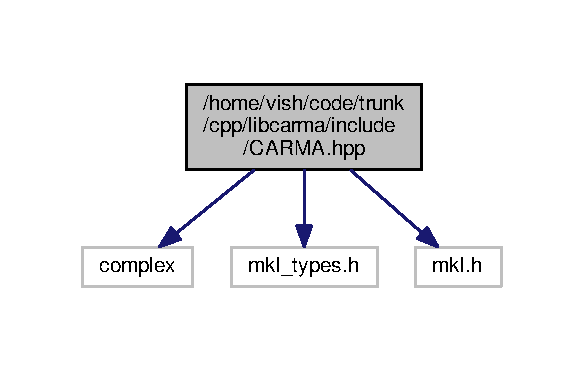
\includegraphics[width=280pt]{_c_a_r_m_a_8hpp__incl}
\end{center}
\end{figure}
This graph shows which files directly or indirectly include this file\-:\nopagebreak
\begin{figure}[H]
\begin{center}
\leavevmode
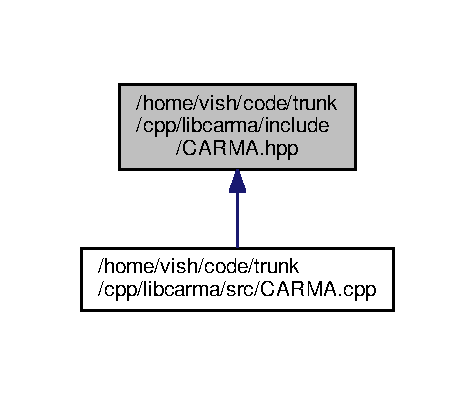
\includegraphics[width=228pt]{_c_a_r_m_a_8hpp__dep__incl}
\end{center}
\end{figure}
\subsection*{Classes}
\begin{DoxyCompactItemize}
\item 
class \hyperlink{class_c_a_r_m_a}{C\-A\-R\-M\-A}
\item 
struct \hyperlink{struct_ln_like_data}{Ln\-Like\-Data}
\item 
struct \hyperlink{struct_ln_like_args}{Ln\-Like\-Args}
\end{DoxyCompactItemize}
\subsection*{Macros}
\begin{DoxyCompactItemize}
\item 
\#define \hyperlink{_c_a_r_m_a_8hpp_a0b45f62ef34311fdb79b8de82d75c0d3}{M\-K\-L\-\_\-\-Complex8}~std\-::complex$<$float$>$
\item 
\#define \hyperlink{_c_a_r_m_a_8hpp_a1fa119034fee07a6d5449926cbb7915a}{M\-K\-L\-\_\-\-Complex16}~std\-::complex$<$double$>$
\end{DoxyCompactItemize}
\subsection*{Functions}
\begin{DoxyCompactItemize}
\item 
double \hyperlink{_c_a_r_m_a_8hpp_a9dd80aa78622e42e58063971be13e31d}{calc\-C\-A\-R\-M\-A\-Ln\-Like} (const vector$<$ double $>$ \&x, vector$<$ double $>$ \&grad, void $\ast$p2\-Args)
\item 
double \hyperlink{_c_a_r_m_a_8hpp_af732e8b64b1fb0da6791e874bd5bafa4}{calc\-C\-A\-R\-M\-A\-Ln\-Like} (double $\ast$walker\-Pos, void $\ast$vd\-Ptr2\-Ln\-Like\-Args)
\item 
double \hyperlink{_c_a_r_m_a_8hpp_ac6c51cd6959e4a7a5ec0557af951daaa}{calc\-Ln\-Like} (const vector$<$ double $>$ \&x, vector$<$ double $>$ \&grad, void $\ast$p2\-Args)
\item 
double \hyperlink{_c_a_r_m_a_8hpp_a9719ae8ef8f4ba7946a78a28412b6273}{calc\-Ln\-Like} (double $\ast$walker\-Pos, void $\ast$vd\-Ptr2\-Ln\-Like\-Args)
\item 
void \hyperlink{_c_a_r_m_a_8hpp_a52e65b8de02410a2382d1c0858c43b25}{zero\-Matrix} (int n\-Rows, int n\-Cols, int $\ast$mat)
\item 
void \hyperlink{_c_a_r_m_a_8hpp_ad06e01d494041ea73f3fb05d5208765f}{zero\-Matrix} (int n\-Rows, int n\-Cols, lapack\-\_\-int $\ast$mat)
\item 
void \hyperlink{_c_a_r_m_a_8hpp_acbdde1f5b60f8f09a2561e877f8279e5}{zero\-Matrix} (int n\-Rows, int n\-Cols, double $\ast$mat)
\item 
void \hyperlink{_c_a_r_m_a_8hpp_aff867598dfd07c509cec6da77c33fb98}{zero\-Matrix} (int n\-Rows, int n\-Cols, complex$<$ double $>$ $\ast$mat)
\item 
void \hyperlink{_c_a_r_m_a_8hpp_adaf529b8047fb0aa639f2aa494b9cfaf}{view\-Matrix} (int n\-Rows, int n\-Cols, double $\ast$mat)
\item 
void \hyperlink{_c_a_r_m_a_8hpp_ab43c14961907b75c90cee7b7fd28a3cc}{view\-Matrix} (int n\-Rows, int n\-Cols, complex$<$ double $>$ $\ast$mat)
\item 
double \hyperlink{_c_a_r_m_a_8hpp_a7a7718261954382ab26f32dae64bf3f4}{dtime} ()
\item 
void \hyperlink{_c_a_r_m_a_8hpp_a0644b006a49b595cc3e4d9cf6dff7303}{kron} (int m, int n, double $\ast$A, int p, int q, double $\ast$B, double $\ast$C)
\end{DoxyCompactItemize}


\subsection{Macro Definition Documentation}
\hypertarget{_c_a_r_m_a_8hpp_a1fa119034fee07a6d5449926cbb7915a}{\index{C\-A\-R\-M\-A.\-hpp@{C\-A\-R\-M\-A.\-hpp}!M\-K\-L\-\_\-\-Complex16@{M\-K\-L\-\_\-\-Complex16}}
\index{M\-K\-L\-\_\-\-Complex16@{M\-K\-L\-\_\-\-Complex16}!CARMA.hpp@{C\-A\-R\-M\-A.\-hpp}}
\subsubsection[{M\-K\-L\-\_\-\-Complex16}]{\setlength{\rightskip}{0pt plus 5cm}\#define M\-K\-L\-\_\-\-Complex16~std\-::complex$<$double$>$}}\label{_c_a_r_m_a_8hpp_a1fa119034fee07a6d5449926cbb7915a}


Definition at line 7 of file C\-A\-R\-M\-A.\-hpp.

\hypertarget{_c_a_r_m_a_8hpp_a0b45f62ef34311fdb79b8de82d75c0d3}{\index{C\-A\-R\-M\-A.\-hpp@{C\-A\-R\-M\-A.\-hpp}!M\-K\-L\-\_\-\-Complex8@{M\-K\-L\-\_\-\-Complex8}}
\index{M\-K\-L\-\_\-\-Complex8@{M\-K\-L\-\_\-\-Complex8}!CARMA.hpp@{C\-A\-R\-M\-A.\-hpp}}
\subsubsection[{M\-K\-L\-\_\-\-Complex8}]{\setlength{\rightskip}{0pt plus 5cm}\#define M\-K\-L\-\_\-\-Complex8~std\-::complex$<$float$>$}}\label{_c_a_r_m_a_8hpp_a0b45f62ef34311fdb79b8de82d75c0d3}


Definition at line 6 of file C\-A\-R\-M\-A.\-hpp.



\subsection{Function Documentation}
\hypertarget{_c_a_r_m_a_8hpp_a9dd80aa78622e42e58063971be13e31d}{\index{C\-A\-R\-M\-A.\-hpp@{C\-A\-R\-M\-A.\-hpp}!calc\-C\-A\-R\-M\-A\-Ln\-Like@{calc\-C\-A\-R\-M\-A\-Ln\-Like}}
\index{calc\-C\-A\-R\-M\-A\-Ln\-Like@{calc\-C\-A\-R\-M\-A\-Ln\-Like}!CARMA.hpp@{C\-A\-R\-M\-A.\-hpp}}
\subsubsection[{calc\-C\-A\-R\-M\-A\-Ln\-Like}]{\setlength{\rightskip}{0pt plus 5cm}double calc\-C\-A\-R\-M\-A\-Ln\-Like (
\begin{DoxyParamCaption}
\item[{const vector$<$ double $>$ \&}]{x, }
\item[{vector$<$ double $>$ \&}]{grad, }
\item[{void $\ast$}]{p2\-Args}
\end{DoxyParamCaption}
)}}\label{_c_a_r_m_a_8hpp_a9dd80aa78622e42e58063971be13e31d}


Definition at line 43 of file C\-A\-R\-M\-A.\-cpp.

\hypertarget{_c_a_r_m_a_8hpp_af732e8b64b1fb0da6791e874bd5bafa4}{\index{C\-A\-R\-M\-A.\-hpp@{C\-A\-R\-M\-A.\-hpp}!calc\-C\-A\-R\-M\-A\-Ln\-Like@{calc\-C\-A\-R\-M\-A\-Ln\-Like}}
\index{calc\-C\-A\-R\-M\-A\-Ln\-Like@{calc\-C\-A\-R\-M\-A\-Ln\-Like}!CARMA.hpp@{C\-A\-R\-M\-A.\-hpp}}
\subsubsection[{calc\-C\-A\-R\-M\-A\-Ln\-Like}]{\setlength{\rightskip}{0pt plus 5cm}double calc\-C\-A\-R\-M\-A\-Ln\-Like (
\begin{DoxyParamCaption}
\item[{double $\ast$}]{walker\-Pos, }
\item[{void $\ast$}]{vd\-Ptr2\-Ln\-Like\-Args}
\end{DoxyParamCaption}
)}}\label{_c_a_r_m_a_8hpp_af732e8b64b1fb0da6791e874bd5bafa4}


Definition at line 100 of file C\-A\-R\-M\-A.\-cpp.

\hypertarget{_c_a_r_m_a_8hpp_ac6c51cd6959e4a7a5ec0557af951daaa}{\index{C\-A\-R\-M\-A.\-hpp@{C\-A\-R\-M\-A.\-hpp}!calc\-Ln\-Like@{calc\-Ln\-Like}}
\index{calc\-Ln\-Like@{calc\-Ln\-Like}!CARMA.hpp@{C\-A\-R\-M\-A.\-hpp}}
\subsubsection[{calc\-Ln\-Like}]{\setlength{\rightskip}{0pt plus 5cm}double calc\-Ln\-Like (
\begin{DoxyParamCaption}
\item[{const vector$<$ double $>$ \&}]{x, }
\item[{vector$<$ double $>$ \&}]{grad, }
\item[{void $\ast$}]{p2\-Args}
\end{DoxyParamCaption}
)}}\label{_c_a_r_m_a_8hpp_ac6c51cd6959e4a7a5ec0557af951daaa}


Definition at line 151 of file C\-A\-R\-M\-A.\-cpp.



Here is the caller graph for this function\-:\nopagebreak
\begin{figure}[H]
\begin{center}
\leavevmode
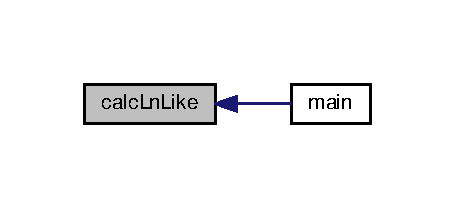
\includegraphics[width=218pt]{_c_a_r_m_a_8hpp_ac6c51cd6959e4a7a5ec0557af951daaa_icgraph}
\end{center}
\end{figure}


\hypertarget{_c_a_r_m_a_8hpp_a9719ae8ef8f4ba7946a78a28412b6273}{\index{C\-A\-R\-M\-A.\-hpp@{C\-A\-R\-M\-A.\-hpp}!calc\-Ln\-Like@{calc\-Ln\-Like}}
\index{calc\-Ln\-Like@{calc\-Ln\-Like}!CARMA.hpp@{C\-A\-R\-M\-A.\-hpp}}
\subsubsection[{calc\-Ln\-Like}]{\setlength{\rightskip}{0pt plus 5cm}double calc\-Ln\-Like (
\begin{DoxyParamCaption}
\item[{double $\ast$}]{walker\-Pos, }
\item[{void $\ast$}]{vd\-Ptr2\-Ln\-Like\-Args}
\end{DoxyParamCaption}
)}}\label{_c_a_r_m_a_8hpp_a9719ae8ef8f4ba7946a78a28412b6273}


Definition at line 208 of file C\-A\-R\-M\-A.\-cpp.

\hypertarget{_c_a_r_m_a_8hpp_a7a7718261954382ab26f32dae64bf3f4}{\index{C\-A\-R\-M\-A.\-hpp@{C\-A\-R\-M\-A.\-hpp}!dtime@{dtime}}
\index{dtime@{dtime}!CARMA.hpp@{C\-A\-R\-M\-A.\-hpp}}
\subsubsection[{dtime}]{\setlength{\rightskip}{0pt plus 5cm}double dtime (
\begin{DoxyParamCaption}
{}
\end{DoxyParamCaption}
)}}\label{_c_a_r_m_a_8hpp_a7a7718261954382ab26f32dae64bf3f4}


Definition at line 318 of file C\-A\-R\-M\-A.\-cpp.



Here is the caller graph for this function\-:\nopagebreak
\begin{figure}[H]
\begin{center}
\leavevmode
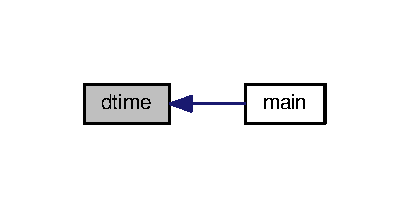
\includegraphics[width=196pt]{_c_a_r_m_a_8hpp_a7a7718261954382ab26f32dae64bf3f4_icgraph}
\end{center}
\end{figure}


\hypertarget{_c_a_r_m_a_8hpp_a0644b006a49b595cc3e4d9cf6dff7303}{\index{C\-A\-R\-M\-A.\-hpp@{C\-A\-R\-M\-A.\-hpp}!kron@{kron}}
\index{kron@{kron}!CARMA.hpp@{C\-A\-R\-M\-A.\-hpp}}
\subsubsection[{kron}]{\setlength{\rightskip}{0pt plus 5cm}void kron (
\begin{DoxyParamCaption}
\item[{int}]{m, }
\item[{int}]{n, }
\item[{double $\ast$}]{A, }
\item[{int}]{p, }
\item[{int}]{q, }
\item[{double $\ast$}]{B, }
\item[{double $\ast$}]{C}
\end{DoxyParamCaption}
)}}\label{_c_a_r_m_a_8hpp_a0644b006a49b595cc3e4d9cf6dff7303}


Definition at line 326 of file C\-A\-R\-M\-A.\-cpp.



Here is the caller graph for this function\-:\nopagebreak
\begin{figure}[H]
\begin{center}
\leavevmode
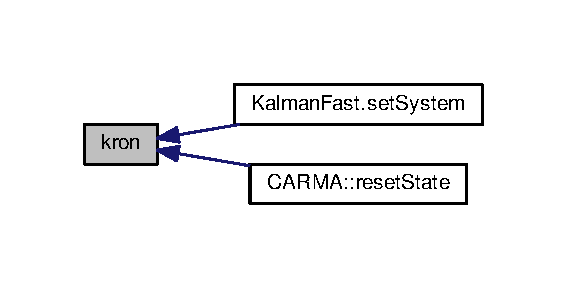
\includegraphics[width=272pt]{_c_a_r_m_a_8hpp_a0644b006a49b595cc3e4d9cf6dff7303_icgraph}
\end{center}
\end{figure}


\hypertarget{_c_a_r_m_a_8hpp_adaf529b8047fb0aa639f2aa494b9cfaf}{\index{C\-A\-R\-M\-A.\-hpp@{C\-A\-R\-M\-A.\-hpp}!view\-Matrix@{view\-Matrix}}
\index{view\-Matrix@{view\-Matrix}!CARMA.hpp@{C\-A\-R\-M\-A.\-hpp}}
\subsubsection[{view\-Matrix}]{\setlength{\rightskip}{0pt plus 5cm}void view\-Matrix (
\begin{DoxyParamCaption}
\item[{int}]{n\-Rows, }
\item[{int}]{n\-Cols, }
\item[{double $\ast$}]{mat}
\end{DoxyParamCaption}
)}}\label{_c_a_r_m_a_8hpp_adaf529b8047fb0aa639f2aa494b9cfaf}


Definition at line 300 of file C\-A\-R\-M\-A.\-cpp.

\hypertarget{_c_a_r_m_a_8hpp_ab43c14961907b75c90cee7b7fd28a3cc}{\index{C\-A\-R\-M\-A.\-hpp@{C\-A\-R\-M\-A.\-hpp}!view\-Matrix@{view\-Matrix}}
\index{view\-Matrix@{view\-Matrix}!CARMA.hpp@{C\-A\-R\-M\-A.\-hpp}}
\subsubsection[{view\-Matrix}]{\setlength{\rightskip}{0pt plus 5cm}void view\-Matrix (
\begin{DoxyParamCaption}
\item[{int}]{n\-Rows, }
\item[{int}]{n\-Cols, }
\item[{complex$<$ double $>$ $\ast$}]{mat}
\end{DoxyParamCaption}
)}}\label{_c_a_r_m_a_8hpp_ab43c14961907b75c90cee7b7fd28a3cc}


Definition at line 309 of file C\-A\-R\-M\-A.\-cpp.

\hypertarget{_c_a_r_m_a_8hpp_a52e65b8de02410a2382d1c0858c43b25}{\index{C\-A\-R\-M\-A.\-hpp@{C\-A\-R\-M\-A.\-hpp}!zero\-Matrix@{zero\-Matrix}}
\index{zero\-Matrix@{zero\-Matrix}!CARMA.hpp@{C\-A\-R\-M\-A.\-hpp}}
\subsubsection[{zero\-Matrix}]{\setlength{\rightskip}{0pt plus 5cm}void zero\-Matrix (
\begin{DoxyParamCaption}
\item[{int}]{n\-Rows, }
\item[{int}]{n\-Cols, }
\item[{int $\ast$}]{mat}
\end{DoxyParamCaption}
)}}\label{_c_a_r_m_a_8hpp_a52e65b8de02410a2382d1c0858c43b25}


Definition at line 268 of file C\-A\-R\-M\-A.\-cpp.

\hypertarget{_c_a_r_m_a_8hpp_ad06e01d494041ea73f3fb05d5208765f}{\index{C\-A\-R\-M\-A.\-hpp@{C\-A\-R\-M\-A.\-hpp}!zero\-Matrix@{zero\-Matrix}}
\index{zero\-Matrix@{zero\-Matrix}!CARMA.hpp@{C\-A\-R\-M\-A.\-hpp}}
\subsubsection[{zero\-Matrix}]{\setlength{\rightskip}{0pt plus 5cm}void zero\-Matrix (
\begin{DoxyParamCaption}
\item[{int}]{n\-Rows, }
\item[{int}]{n\-Cols, }
\item[{lapack\-\_\-int $\ast$}]{mat}
\end{DoxyParamCaption}
)}}\label{_c_a_r_m_a_8hpp_ad06e01d494041ea73f3fb05d5208765f}


Definition at line 276 of file C\-A\-R\-M\-A.\-cpp.

\hypertarget{_c_a_r_m_a_8hpp_acbdde1f5b60f8f09a2561e877f8279e5}{\index{C\-A\-R\-M\-A.\-hpp@{C\-A\-R\-M\-A.\-hpp}!zero\-Matrix@{zero\-Matrix}}
\index{zero\-Matrix@{zero\-Matrix}!CARMA.hpp@{C\-A\-R\-M\-A.\-hpp}}
\subsubsection[{zero\-Matrix}]{\setlength{\rightskip}{0pt plus 5cm}void zero\-Matrix (
\begin{DoxyParamCaption}
\item[{int}]{n\-Rows, }
\item[{int}]{n\-Cols, }
\item[{double $\ast$}]{mat}
\end{DoxyParamCaption}
)}}\label{_c_a_r_m_a_8hpp_acbdde1f5b60f8f09a2561e877f8279e5}


Definition at line 284 of file C\-A\-R\-M\-A.\-cpp.

\hypertarget{_c_a_r_m_a_8hpp_aff867598dfd07c509cec6da77c33fb98}{\index{C\-A\-R\-M\-A.\-hpp@{C\-A\-R\-M\-A.\-hpp}!zero\-Matrix@{zero\-Matrix}}
\index{zero\-Matrix@{zero\-Matrix}!CARMA.hpp@{C\-A\-R\-M\-A.\-hpp}}
\subsubsection[{zero\-Matrix}]{\setlength{\rightskip}{0pt plus 5cm}void zero\-Matrix (
\begin{DoxyParamCaption}
\item[{int}]{n\-Rows, }
\item[{int}]{n\-Cols, }
\item[{complex$<$ double $>$ $\ast$}]{mat}
\end{DoxyParamCaption}
)}}\label{_c_a_r_m_a_8hpp_aff867598dfd07c509cec6da77c33fb98}


Definition at line 292 of file C\-A\-R\-M\-A.\-cpp.


\hypertarget{_constants_8hpp}{\section{/home/vish/code/trunk/cpp/libcarma/cython/include/\-Constants.hpp File Reference}
\label{_constants_8hpp}\index{/home/vish/code/trunk/cpp/libcarma/cython/include/\-Constants.\-hpp@{/home/vish/code/trunk/cpp/libcarma/cython/include/\-Constants.\-hpp}}
}
{\ttfamily \#include $<$complex$>$}\\*
Include dependency graph for Constants.\-hpp\-:
This graph shows which files directly or indirectly include this file\-:
\subsection*{Variables}
\begin{DoxyCompactItemize}
\item 
complex$<$ double $>$ \hyperlink{_constants_8hpp_a1429bd49fdfa9d3e410e025876d72d0e}{complex\-Zero}
\item 
complex$<$ double $>$ \hyperlink{_constants_8hpp_a7fcae12bee2bf97db614c980f2912ded}{complex\-One}
\item 
double \hyperlink{_constants_8hpp_a31c17cc321db72d5ab448b71ea92792f}{pi}
\item 
double \hyperlink{_constants_8hpp_a18bbe41d56bab00212fd0e8e733e9f1f}{pi\-Sq}
\item 
double \hyperlink{_constants_8hpp_ab17e17fb32b792781b807505e7f60c9c}{e}
\item 
double \hyperlink{_constants_8hpp_a5ce1018aef28e71271ae3b4431210720}{infinite\-Val}
\item 
double \hyperlink{_constants_8hpp_a67783a2c4f670ee5a9dadcf428324d32}{G}
\item 
double \hyperlink{_constants_8hpp_a2c09e929a6ea340fc9653cca414b11d3}{c}
\item 
double \hyperlink{_constants_8hpp_a8497a2d27908c87901466c9de72ff8d8}{A\-U}
\item 
double \hyperlink{_constants_8hpp_a2e08042cd1e7eb1861e7115f34fa3acb}{Parsec}
\item 
double \hyperlink{_constants_8hpp_a187ad5035a30f1230f63152e677791ba}{Day}
\item 
double \hyperlink{_constants_8hpp_aa2047f98d2c2eecb4bfe0d2bd43ac10e}{Year}
\item 
double \hyperlink{_constants_8hpp_a81120f2278cac2eb2b1cb85782c83024}{kms2ms}
\item 
double \hyperlink{_constants_8hpp_ada9035453156e0ae346332fde905c274}{Solar\-Mass}
\item 
double \hyperlink{_constants_8hpp_a798a374e513280a7d37661626aab93d5}{Solar\-Mass\-Per\-Cubic\-Parsec}
\item 
double \hyperlink{_constants_8hpp_a6a9e5bbdf108936466078a267b5acd51}{integration\-Time}
\item 
double \hyperlink{_constants_8hpp_abd52f1ed1ece35cffe3fc3e4180ca0f3}{read\-Time}
\item 
int \hyperlink{_constants_8hpp_aeab23e8ce3743c4e554e657ce55c5305}{num\-Integrations\-S\-C}
\item 
int \hyperlink{_constants_8hpp_a045a70c6ff8d3041c66cb29263a0f815}{num\-Integrations\-L\-C}
\item 
double \hyperlink{_constants_8hpp_a3b68866972010d697c2f9e3def43a8c4}{sampling\-Interval\-S\-C}
\item 
double \hyperlink{_constants_8hpp_a7eec0eac1517df1522a3775fc44ddf7d}{sampling\-Interval\-L\-C}
\item 
double \hyperlink{_constants_8hpp_abae737372bcd2caafbf77434f3b0ed97}{sampling\-Frequency\-S\-C}
\item 
double \hyperlink{_constants_8hpp_a102f4d453dc44d0a812bde4a0c8c19c8}{sampling\-Frequency\-L\-C}
\item 
double \hyperlink{_constants_8hpp_a29c58ec25452277c1661f674327a77a4}{Nyquist\-Frequency\-S\-C}
\item 
double \hyperlink{_constants_8hpp_a598be37cc4a0d559305212b7e8c21045}{Nyquist\-Frequency\-L\-C}
\item 
double \hyperlink{_constants_8hpp_ad273a878a46f52a8c720ef7eae03ae4f}{sec\-Per\-Sidereal\-Day}
\item 
double \hyperlink{_constants_8hpp_ad55d7bc1d7b5c686f6197b02498e4eaf}{sc\-Cadence}
\item 
double \hyperlink{_constants_8hpp_ac18142dbc207474c073432f4b28424b9}{lc\-Cadence}
\item 
double \hyperlink{_constants_8hpp_a6a5210c2bcb5149c1073568e5c8d6599}{log2\-Of\-E}
\item 
double \hyperlink{_constants_8hpp_a2b27190acf3cc471e389bb8173544658}{log2\-Pi}
\end{DoxyCompactItemize}


\subsection{Variable Documentation}
\hypertarget{_constants_8hpp_a8497a2d27908c87901466c9de72ff8d8}{\index{Constants.\-hpp@{Constants.\-hpp}!A\-U@{A\-U}}
\index{A\-U@{A\-U}!Constants.hpp@{Constants.\-hpp}}
\subsubsection[{A\-U}]{\setlength{\rightskip}{0pt plus 5cm}double A\-U}}\label{_constants_8hpp_a8497a2d27908c87901466c9de72ff8d8}


Definition at line 27 of file binary\-S\-M\-B\-H\-Demo.\-py.

\hypertarget{_constants_8hpp_a2c09e929a6ea340fc9653cca414b11d3}{\index{Constants.\-hpp@{Constants.\-hpp}!c@{c}}
\index{c@{c}!Constants.hpp@{Constants.\-hpp}}
\subsubsection[{c}]{\setlength{\rightskip}{0pt plus 5cm}double c}}\label{_constants_8hpp_a2c09e929a6ea340fc9653cca414b11d3}


Definition at line 26 of file binary\-S\-M\-B\-H\-Demo.\-py.

\hypertarget{_constants_8hpp_a7fcae12bee2bf97db614c980f2912ded}{\index{Constants.\-hpp@{Constants.\-hpp}!complex\-One@{complex\-One}}
\index{complex\-One@{complex\-One}!Constants.hpp@{Constants.\-hpp}}
\subsubsection[{complex\-One}]{\setlength{\rightskip}{0pt plus 5cm}complex$<$double$>$ complex\-One}}\label{_constants_8hpp_a7fcae12bee2bf97db614c980f2912ded}
\hypertarget{_constants_8hpp_a1429bd49fdfa9d3e410e025876d72d0e}{\index{Constants.\-hpp@{Constants.\-hpp}!complex\-Zero@{complex\-Zero}}
\index{complex\-Zero@{complex\-Zero}!Constants.hpp@{Constants.\-hpp}}
\subsubsection[{complex\-Zero}]{\setlength{\rightskip}{0pt plus 5cm}complex$<$double$>$ complex\-Zero}}\label{_constants_8hpp_a1429bd49fdfa9d3e410e025876d72d0e}
\hypertarget{_constants_8hpp_a187ad5035a30f1230f63152e677791ba}{\index{Constants.\-hpp@{Constants.\-hpp}!Day@{Day}}
\index{Day@{Day}!Constants.hpp@{Constants.\-hpp}}
\subsubsection[{Day}]{\setlength{\rightskip}{0pt plus 5cm}double Day}}\label{_constants_8hpp_a187ad5035a30f1230f63152e677791ba}


Definition at line 30 of file binary\-S\-M\-B\-H\-Demo.\-py.

\hypertarget{_constants_8hpp_ab17e17fb32b792781b807505e7f60c9c}{\index{Constants.\-hpp@{Constants.\-hpp}!e@{e}}
\index{e@{e}!Constants.hpp@{Constants.\-hpp}}
\subsubsection[{e}]{\setlength{\rightskip}{0pt plus 5cm}double e}}\label{_constants_8hpp_ab17e17fb32b792781b807505e7f60c9c}
\hypertarget{_constants_8hpp_a67783a2c4f670ee5a9dadcf428324d32}{\index{Constants.\-hpp@{Constants.\-hpp}!G@{G}}
\index{G@{G}!Constants.hpp@{Constants.\-hpp}}
\subsubsection[{G}]{\setlength{\rightskip}{0pt plus 5cm}double G}}\label{_constants_8hpp_a67783a2c4f670ee5a9dadcf428324d32}


Definition at line 25 of file binary\-S\-M\-B\-H\-Demo.\-py.

\hypertarget{_constants_8hpp_a5ce1018aef28e71271ae3b4431210720}{\index{Constants.\-hpp@{Constants.\-hpp}!infinite\-Val@{infinite\-Val}}
\index{infinite\-Val@{infinite\-Val}!Constants.hpp@{Constants.\-hpp}}
\subsubsection[{infinite\-Val}]{\setlength{\rightskip}{0pt plus 5cm}double infinite\-Val}}\label{_constants_8hpp_a5ce1018aef28e71271ae3b4431210720}
\hypertarget{_constants_8hpp_a6a9e5bbdf108936466078a267b5acd51}{\index{Constants.\-hpp@{Constants.\-hpp}!integration\-Time@{integration\-Time}}
\index{integration\-Time@{integration\-Time}!Constants.hpp@{Constants.\-hpp}}
\subsubsection[{integration\-Time}]{\setlength{\rightskip}{0pt plus 5cm}double integration\-Time}}\label{_constants_8hpp_a6a9e5bbdf108936466078a267b5acd51}
\hypertarget{_constants_8hpp_a81120f2278cac2eb2b1cb85782c83024}{\index{Constants.\-hpp@{Constants.\-hpp}!kms2ms@{kms2ms}}
\index{kms2ms@{kms2ms}!Constants.hpp@{Constants.\-hpp}}
\subsubsection[{kms2ms}]{\setlength{\rightskip}{0pt plus 5cm}double kms2ms}}\label{_constants_8hpp_a81120f2278cac2eb2b1cb85782c83024}


Definition at line 33 of file binary\-S\-M\-B\-H\-Demo.\-py.

\hypertarget{_constants_8hpp_ac18142dbc207474c073432f4b28424b9}{\index{Constants.\-hpp@{Constants.\-hpp}!lc\-Cadence@{lc\-Cadence}}
\index{lc\-Cadence@{lc\-Cadence}!Constants.hpp@{Constants.\-hpp}}
\subsubsection[{lc\-Cadence}]{\setlength{\rightskip}{0pt plus 5cm}double lc\-Cadence}}\label{_constants_8hpp_ac18142dbc207474c073432f4b28424b9}
\hypertarget{_constants_8hpp_a6a5210c2bcb5149c1073568e5c8d6599}{\index{Constants.\-hpp@{Constants.\-hpp}!log2\-Of\-E@{log2\-Of\-E}}
\index{log2\-Of\-E@{log2\-Of\-E}!Constants.hpp@{Constants.\-hpp}}
\subsubsection[{log2\-Of\-E}]{\setlength{\rightskip}{0pt plus 5cm}double log2\-Of\-E}}\label{_constants_8hpp_a6a5210c2bcb5149c1073568e5c8d6599}
\hypertarget{_constants_8hpp_a2b27190acf3cc471e389bb8173544658}{\index{Constants.\-hpp@{Constants.\-hpp}!log2\-Pi@{log2\-Pi}}
\index{log2\-Pi@{log2\-Pi}!Constants.hpp@{Constants.\-hpp}}
\subsubsection[{log2\-Pi}]{\setlength{\rightskip}{0pt plus 5cm}double log2\-Pi}}\label{_constants_8hpp_a2b27190acf3cc471e389bb8173544658}
\hypertarget{_constants_8hpp_a045a70c6ff8d3041c66cb29263a0f815}{\index{Constants.\-hpp@{Constants.\-hpp}!num\-Integrations\-L\-C@{num\-Integrations\-L\-C}}
\index{num\-Integrations\-L\-C@{num\-Integrations\-L\-C}!Constants.hpp@{Constants.\-hpp}}
\subsubsection[{num\-Integrations\-L\-C}]{\setlength{\rightskip}{0pt plus 5cm}int num\-Integrations\-L\-C}}\label{_constants_8hpp_a045a70c6ff8d3041c66cb29263a0f815}
\hypertarget{_constants_8hpp_aeab23e8ce3743c4e554e657ce55c5305}{\index{Constants.\-hpp@{Constants.\-hpp}!num\-Integrations\-S\-C@{num\-Integrations\-S\-C}}
\index{num\-Integrations\-S\-C@{num\-Integrations\-S\-C}!Constants.hpp@{Constants.\-hpp}}
\subsubsection[{num\-Integrations\-S\-C}]{\setlength{\rightskip}{0pt plus 5cm}int num\-Integrations\-S\-C}}\label{_constants_8hpp_aeab23e8ce3743c4e554e657ce55c5305}
\hypertarget{_constants_8hpp_a598be37cc4a0d559305212b7e8c21045}{\index{Constants.\-hpp@{Constants.\-hpp}!Nyquist\-Frequency\-L\-C@{Nyquist\-Frequency\-L\-C}}
\index{Nyquist\-Frequency\-L\-C@{Nyquist\-Frequency\-L\-C}!Constants.hpp@{Constants.\-hpp}}
\subsubsection[{Nyquist\-Frequency\-L\-C}]{\setlength{\rightskip}{0pt plus 5cm}double Nyquist\-Frequency\-L\-C}}\label{_constants_8hpp_a598be37cc4a0d559305212b7e8c21045}
\hypertarget{_constants_8hpp_a29c58ec25452277c1661f674327a77a4}{\index{Constants.\-hpp@{Constants.\-hpp}!Nyquist\-Frequency\-S\-C@{Nyquist\-Frequency\-S\-C}}
\index{Nyquist\-Frequency\-S\-C@{Nyquist\-Frequency\-S\-C}!Constants.hpp@{Constants.\-hpp}}
\subsubsection[{Nyquist\-Frequency\-S\-C}]{\setlength{\rightskip}{0pt plus 5cm}double Nyquist\-Frequency\-S\-C}}\label{_constants_8hpp_a29c58ec25452277c1661f674327a77a4}
\hypertarget{_constants_8hpp_a2e08042cd1e7eb1861e7115f34fa3acb}{\index{Constants.\-hpp@{Constants.\-hpp}!Parsec@{Parsec}}
\index{Parsec@{Parsec}!Constants.hpp@{Constants.\-hpp}}
\subsubsection[{Parsec}]{\setlength{\rightskip}{0pt plus 5cm}double Parsec}}\label{_constants_8hpp_a2e08042cd1e7eb1861e7115f34fa3acb}


Definition at line 28 of file binary\-S\-M\-B\-H\-Demo.\-py.

\hypertarget{_constants_8hpp_a31c17cc321db72d5ab448b71ea92792f}{\index{Constants.\-hpp@{Constants.\-hpp}!pi@{pi}}
\index{pi@{pi}!Constants.hpp@{Constants.\-hpp}}
\subsubsection[{pi}]{\setlength{\rightskip}{0pt plus 5cm}double pi}}\label{_constants_8hpp_a31c17cc321db72d5ab448b71ea92792f}
\hypertarget{_constants_8hpp_a18bbe41d56bab00212fd0e8e733e9f1f}{\index{Constants.\-hpp@{Constants.\-hpp}!pi\-Sq@{pi\-Sq}}
\index{pi\-Sq@{pi\-Sq}!Constants.hpp@{Constants.\-hpp}}
\subsubsection[{pi\-Sq}]{\setlength{\rightskip}{0pt plus 5cm}double pi\-Sq}}\label{_constants_8hpp_a18bbe41d56bab00212fd0e8e733e9f1f}
\hypertarget{_constants_8hpp_abd52f1ed1ece35cffe3fc3e4180ca0f3}{\index{Constants.\-hpp@{Constants.\-hpp}!read\-Time@{read\-Time}}
\index{read\-Time@{read\-Time}!Constants.hpp@{Constants.\-hpp}}
\subsubsection[{read\-Time}]{\setlength{\rightskip}{0pt plus 5cm}double read\-Time}}\label{_constants_8hpp_abd52f1ed1ece35cffe3fc3e4180ca0f3}
\hypertarget{_constants_8hpp_a102f4d453dc44d0a812bde4a0c8c19c8}{\index{Constants.\-hpp@{Constants.\-hpp}!sampling\-Frequency\-L\-C@{sampling\-Frequency\-L\-C}}
\index{sampling\-Frequency\-L\-C@{sampling\-Frequency\-L\-C}!Constants.hpp@{Constants.\-hpp}}
\subsubsection[{sampling\-Frequency\-L\-C}]{\setlength{\rightskip}{0pt plus 5cm}double sampling\-Frequency\-L\-C}}\label{_constants_8hpp_a102f4d453dc44d0a812bde4a0c8c19c8}
\hypertarget{_constants_8hpp_abae737372bcd2caafbf77434f3b0ed97}{\index{Constants.\-hpp@{Constants.\-hpp}!sampling\-Frequency\-S\-C@{sampling\-Frequency\-S\-C}}
\index{sampling\-Frequency\-S\-C@{sampling\-Frequency\-S\-C}!Constants.hpp@{Constants.\-hpp}}
\subsubsection[{sampling\-Frequency\-S\-C}]{\setlength{\rightskip}{0pt plus 5cm}double sampling\-Frequency\-S\-C}}\label{_constants_8hpp_abae737372bcd2caafbf77434f3b0ed97}
\hypertarget{_constants_8hpp_a7eec0eac1517df1522a3775fc44ddf7d}{\index{Constants.\-hpp@{Constants.\-hpp}!sampling\-Interval\-L\-C@{sampling\-Interval\-L\-C}}
\index{sampling\-Interval\-L\-C@{sampling\-Interval\-L\-C}!Constants.hpp@{Constants.\-hpp}}
\subsubsection[{sampling\-Interval\-L\-C}]{\setlength{\rightskip}{0pt plus 5cm}double sampling\-Interval\-L\-C}}\label{_constants_8hpp_a7eec0eac1517df1522a3775fc44ddf7d}
\hypertarget{_constants_8hpp_a3b68866972010d697c2f9e3def43a8c4}{\index{Constants.\-hpp@{Constants.\-hpp}!sampling\-Interval\-S\-C@{sampling\-Interval\-S\-C}}
\index{sampling\-Interval\-S\-C@{sampling\-Interval\-S\-C}!Constants.hpp@{Constants.\-hpp}}
\subsubsection[{sampling\-Interval\-S\-C}]{\setlength{\rightskip}{0pt plus 5cm}double sampling\-Interval\-S\-C}}\label{_constants_8hpp_a3b68866972010d697c2f9e3def43a8c4}
\hypertarget{_constants_8hpp_ad55d7bc1d7b5c686f6197b02498e4eaf}{\index{Constants.\-hpp@{Constants.\-hpp}!sc\-Cadence@{sc\-Cadence}}
\index{sc\-Cadence@{sc\-Cadence}!Constants.hpp@{Constants.\-hpp}}
\subsubsection[{sc\-Cadence}]{\setlength{\rightskip}{0pt plus 5cm}double sc\-Cadence}}\label{_constants_8hpp_ad55d7bc1d7b5c686f6197b02498e4eaf}
\hypertarget{_constants_8hpp_ad273a878a46f52a8c720ef7eae03ae4f}{\index{Constants.\-hpp@{Constants.\-hpp}!sec\-Per\-Sidereal\-Day@{sec\-Per\-Sidereal\-Day}}
\index{sec\-Per\-Sidereal\-Day@{sec\-Per\-Sidereal\-Day}!Constants.hpp@{Constants.\-hpp}}
\subsubsection[{sec\-Per\-Sidereal\-Day}]{\setlength{\rightskip}{0pt plus 5cm}double sec\-Per\-Sidereal\-Day}}\label{_constants_8hpp_ad273a878a46f52a8c720ef7eae03ae4f}
\hypertarget{_constants_8hpp_ada9035453156e0ae346332fde905c274}{\index{Constants.\-hpp@{Constants.\-hpp}!Solar\-Mass@{Solar\-Mass}}
\index{Solar\-Mass@{Solar\-Mass}!Constants.hpp@{Constants.\-hpp}}
\subsubsection[{Solar\-Mass}]{\setlength{\rightskip}{0pt plus 5cm}double Solar\-Mass}}\label{_constants_8hpp_ada9035453156e0ae346332fde905c274}


Definition at line 32 of file binary\-S\-M\-B\-H\-Demo.\-py.

\hypertarget{_constants_8hpp_a798a374e513280a7d37661626aab93d5}{\index{Constants.\-hpp@{Constants.\-hpp}!Solar\-Mass\-Per\-Cubic\-Parsec@{Solar\-Mass\-Per\-Cubic\-Parsec}}
\index{Solar\-Mass\-Per\-Cubic\-Parsec@{Solar\-Mass\-Per\-Cubic\-Parsec}!Constants.hpp@{Constants.\-hpp}}
\subsubsection[{Solar\-Mass\-Per\-Cubic\-Parsec}]{\setlength{\rightskip}{0pt plus 5cm}double Solar\-Mass\-Per\-Cubic\-Parsec}}\label{_constants_8hpp_a798a374e513280a7d37661626aab93d5}


Definition at line 34 of file binary\-S\-M\-B\-H\-Demo.\-py.

\hypertarget{_constants_8hpp_aa2047f98d2c2eecb4bfe0d2bd43ac10e}{\index{Constants.\-hpp@{Constants.\-hpp}!Year@{Year}}
\index{Year@{Year}!Constants.hpp@{Constants.\-hpp}}
\subsubsection[{Year}]{\setlength{\rightskip}{0pt plus 5cm}double Year}}\label{_constants_8hpp_aa2047f98d2c2eecb4bfe0d2bd43ac10e}


Definition at line 29 of file binary\-S\-M\-B\-H\-Demo.\-py.


\hypertarget{_l_c_8hpp}{\section{/home/vish/code/trunk/cpp/libcarma/cython/include/\-L\-C.hpp File Reference}
\label{_l_c_8hpp}\index{/home/vish/code/trunk/cpp/libcarma/cython/include/\-L\-C.\-hpp@{/home/vish/code/trunk/cpp/libcarma/cython/include/\-L\-C.\-hpp}}
}
{\ttfamily \#include $<$complex$>$}\\*
{\ttfamily \#include $<$mkl\-\_\-types.\-h$>$}\\*
{\ttfamily \#include $<$mkl.\-h$>$}\\*
Include dependency graph for L\-C.\-hpp\-:
This graph shows which files directly or indirectly include this file\-:
\subsection*{Classes}
\begin{DoxyCompactItemize}
\item 
class \hyperlink{class_l_c_data}{L\-C\-Data}
\end{DoxyCompactItemize}
\subsection*{Macros}
\begin{DoxyCompactItemize}
\item 
\#define \hyperlink{_l_c_8hpp_a0b45f62ef34311fdb79b8de82d75c0d3}{M\-K\-L\-\_\-\-Complex8}~std\-::complex$<$float$>$
\item 
\#define \hyperlink{_l_c_8hpp_a1fa119034fee07a6d5449926cbb7915a}{M\-K\-L\-\_\-\-Complex16}~std\-::complex$<$double$>$
\end{DoxyCompactItemize}


\subsection{Macro Definition Documentation}
\hypertarget{_l_c_8hpp_a1fa119034fee07a6d5449926cbb7915a}{\index{L\-C.\-hpp@{L\-C.\-hpp}!M\-K\-L\-\_\-\-Complex16@{M\-K\-L\-\_\-\-Complex16}}
\index{M\-K\-L\-\_\-\-Complex16@{M\-K\-L\-\_\-\-Complex16}!LC.hpp@{L\-C.\-hpp}}
\subsubsection[{M\-K\-L\-\_\-\-Complex16}]{\setlength{\rightskip}{0pt plus 5cm}\#define M\-K\-L\-\_\-\-Complex16~std\-::complex$<$double$>$}}\label{_l_c_8hpp_a1fa119034fee07a6d5449926cbb7915a}


Definition at line 7 of file L\-C.\-hpp.

\hypertarget{_l_c_8hpp_a0b45f62ef34311fdb79b8de82d75c0d3}{\index{L\-C.\-hpp@{L\-C.\-hpp}!M\-K\-L\-\_\-\-Complex8@{M\-K\-L\-\_\-\-Complex8}}
\index{M\-K\-L\-\_\-\-Complex8@{M\-K\-L\-\_\-\-Complex8}!LC.hpp@{L\-C.\-hpp}}
\subsubsection[{M\-K\-L\-\_\-\-Complex8}]{\setlength{\rightskip}{0pt plus 5cm}\#define M\-K\-L\-\_\-\-Complex8~std\-::complex$<$float$>$}}\label{_l_c_8hpp_a0b45f62ef34311fdb79b8de82d75c0d3}


Definition at line 6 of file L\-C.\-hpp.


\hypertarget{_m_c_m_c_8hpp}{\section{/home/vish/code/trunk/cpp/libcarma/cython/include/\-M\-C\-M\-C.hpp File Reference}
\label{_m_c_m_c_8hpp}\index{/home/vish/code/trunk/cpp/libcarma/cython/include/\-M\-C\-M\-C.\-hpp@{/home/vish/code/trunk/cpp/libcarma/cython/include/\-M\-C\-M\-C.\-hpp}}
}
This graph shows which files directly or indirectly include this file\-:
\subsection*{Classes}
\begin{DoxyCompactItemize}
\item 
class \hyperlink{class_ensemble_sampler}{Ensemble\-Sampler}
\end{DoxyCompactItemize}

\hypertarget{rdrand_8hpp}{\section{/home/vish/code/trunk/cpp/libcarma/cython/include/rdrand.hpp File Reference}
\label{rdrand_8hpp}\index{/home/vish/code/trunk/cpp/libcarma/cython/include/rdrand.\-hpp@{/home/vish/code/trunk/cpp/libcarma/cython/include/rdrand.\-hpp}}
}
{\ttfamily \#include $<$stdint.\-h$>$}\\*
Include dependency graph for rdrand.\-hpp\-:
This graph shows which files directly or indirectly include this file\-:
\subsection*{Macros}
\begin{DoxyCompactItemize}
\item 
\#define \hyperlink{rdrand_8hpp_a8e20c349766b3e174dc5e27bd0db79fc}{R\-D\-R\-A\-N\-D\-\_\-\-S\-U\-C\-C\-E\-S\-S}~1
\item 
\#define \hyperlink{rdrand_8hpp_a1dd7849babc67ef0652c6fb0290e1004}{R\-D\-R\-A\-N\-D\-\_\-\-N\-O\-T\-\_\-\-R\-E\-A\-D\-Y}~-\/1
\item 
\#define \hyperlink{rdrand_8hpp_ad131f54060ea28be27c3c7bad0690e78}{R\-D\-R\-A\-N\-D\-\_\-\-S\-U\-P\-P\-O\-R\-T\-E\-D}~-\/2
\item 
\#define \hyperlink{rdrand_8hpp_a9575c78908cc2224ce4413cbd965640c}{R\-D\-R\-A\-N\-D\-\_\-\-U\-N\-S\-U\-P\-P\-O\-R\-T\-E\-D}~-\/3
\item 
\#define \hyperlink{rdrand_8hpp_a5c08b02f43bf40a193fdfcc838c185cd}{R\-D\-R\-A\-N\-D\-\_\-\-S\-U\-P\-P\-O\-R\-T\-\_\-\-U\-N\-K\-N\-O\-W\-N}~-\/4
\end{DoxyCompactItemize}
\subsection*{Functions}
\begin{DoxyCompactItemize}
\item 
int \hyperlink{rdrand_8hpp_ac0b6836005a9eeaa7fc22e8ec128da4c}{rdrand\-\_\-16} (uint16\-\_\-t $\ast$x, int retry)
\begin{DoxyCompactList}\small\item\em Calls rdrand for a 16-\/bit result. \end{DoxyCompactList}\item 
int \hyperlink{rdrand_8hpp_ae5322e4aa5e55c40875b980638726001}{rdrand\-\_\-32} (uint32\-\_\-t $\ast$x, int retry)
\begin{DoxyCompactList}\small\item\em Calls rdrand for a 32-\/byte result. \end{DoxyCompactList}\item 
int \hyperlink{rdrand_8hpp_a2982203449ab462050e54165e8f091db}{rdrand\-\_\-64} (uint64\-\_\-t $\ast$x, int retry)
\begin{DoxyCompactList}\small\item\em Calls rdrand for a 64-\/byte result. \end{DoxyCompactList}\item 
int \hyperlink{rdrand_8hpp_af3417f8f6b25ffb090aa102e4d223c05}{rdrand\-\_\-get\-\_\-n\-\_\-64} (unsigned int n, uint64\-\_\-t $\ast$x)
\begin{DoxyCompactList}\small\item\em Calls rdrand to obtain multiple 64-\/byte results. \end{DoxyCompactList}\item 
int \hyperlink{rdrand_8hpp_a274f8a8206b8113d441df7f4df5f00de}{rdrand\-\_\-get\-\_\-n\-\_\-32} (unsigned int n, uint32\-\_\-t $\ast$x)
\begin{DoxyCompactList}\small\item\em Calls rdrand to obtain multiple 32-\/byte results. \end{DoxyCompactList}\item 
int \hyperlink{rdrand_8hpp_a1a468804afabc5a50899235998bd23d6}{rdrand\-\_\-get\-\_\-bytes} (unsigned int n, unsigned char $\ast$buffer)
\begin{DoxyCompactList}\small\item\em Calls rdrand to fill a buffer of arbitrary size with random bytes. \end{DoxyCompactList}\end{DoxyCompactItemize}


\subsection{Macro Definition Documentation}
\hypertarget{rdrand_8hpp_a1dd7849babc67ef0652c6fb0290e1004}{\index{rdrand.\-hpp@{rdrand.\-hpp}!R\-D\-R\-A\-N\-D\-\_\-\-N\-O\-T\-\_\-\-R\-E\-A\-D\-Y@{R\-D\-R\-A\-N\-D\-\_\-\-N\-O\-T\-\_\-\-R\-E\-A\-D\-Y}}
\index{R\-D\-R\-A\-N\-D\-\_\-\-N\-O\-T\-\_\-\-R\-E\-A\-D\-Y@{R\-D\-R\-A\-N\-D\-\_\-\-N\-O\-T\-\_\-\-R\-E\-A\-D\-Y}!rdrand.hpp@{rdrand.\-hpp}}
\subsubsection[{R\-D\-R\-A\-N\-D\-\_\-\-N\-O\-T\-\_\-\-R\-E\-A\-D\-Y}]{\setlength{\rightskip}{0pt plus 5cm}\#define R\-D\-R\-A\-N\-D\-\_\-\-N\-O\-T\-\_\-\-R\-E\-A\-D\-Y~-\/1}}\label{rdrand_8hpp_a1dd7849babc67ef0652c6fb0290e1004}
The rdrand call was unsuccessful, the hardware was not ready, and a random number was not returned. 

Definition at line 61 of file rdrand.\-hpp.

\hypertarget{rdrand_8hpp_a8e20c349766b3e174dc5e27bd0db79fc}{\index{rdrand.\-hpp@{rdrand.\-hpp}!R\-D\-R\-A\-N\-D\-\_\-\-S\-U\-C\-C\-E\-S\-S@{R\-D\-R\-A\-N\-D\-\_\-\-S\-U\-C\-C\-E\-S\-S}}
\index{R\-D\-R\-A\-N\-D\-\_\-\-S\-U\-C\-C\-E\-S\-S@{R\-D\-R\-A\-N\-D\-\_\-\-S\-U\-C\-C\-E\-S\-S}!rdrand.hpp@{rdrand.\-hpp}}
\subsubsection[{R\-D\-R\-A\-N\-D\-\_\-\-S\-U\-C\-C\-E\-S\-S}]{\setlength{\rightskip}{0pt plus 5cm}\#define R\-D\-R\-A\-N\-D\-\_\-\-S\-U\-C\-C\-E\-S\-S~1}}\label{rdrand_8hpp_a8e20c349766b3e174dc5e27bd0db79fc}
The rdrand call was successful, the hardware was ready, and a random number was returned. 

Definition at line 55 of file rdrand.\-hpp.

\hypertarget{rdrand_8hpp_a5c08b02f43bf40a193fdfcc838c185cd}{\index{rdrand.\-hpp@{rdrand.\-hpp}!R\-D\-R\-A\-N\-D\-\_\-\-S\-U\-P\-P\-O\-R\-T\-\_\-\-U\-N\-K\-N\-O\-W\-N@{R\-D\-R\-A\-N\-D\-\_\-\-S\-U\-P\-P\-O\-R\-T\-\_\-\-U\-N\-K\-N\-O\-W\-N}}
\index{R\-D\-R\-A\-N\-D\-\_\-\-S\-U\-P\-P\-O\-R\-T\-\_\-\-U\-N\-K\-N\-O\-W\-N@{R\-D\-R\-A\-N\-D\-\_\-\-S\-U\-P\-P\-O\-R\-T\-\_\-\-U\-N\-K\-N\-O\-W\-N}!rdrand.hpp@{rdrand.\-hpp}}
\subsubsection[{R\-D\-R\-A\-N\-D\-\_\-\-S\-U\-P\-P\-O\-R\-T\-\_\-\-U\-N\-K\-N\-O\-W\-N}]{\setlength{\rightskip}{0pt plus 5cm}\#define R\-D\-R\-A\-N\-D\-\_\-\-S\-U\-P\-P\-O\-R\-T\-\_\-\-U\-N\-K\-N\-O\-W\-N~-\/4}}\label{rdrand_8hpp_a5c08b02f43bf40a193fdfcc838c185cd}
Whether or not the hardware supports the rdrand instruction is unknown 

Definition at line 76 of file rdrand.\-hpp.

\hypertarget{rdrand_8hpp_ad131f54060ea28be27c3c7bad0690e78}{\index{rdrand.\-hpp@{rdrand.\-hpp}!R\-D\-R\-A\-N\-D\-\_\-\-S\-U\-P\-P\-O\-R\-T\-E\-D@{R\-D\-R\-A\-N\-D\-\_\-\-S\-U\-P\-P\-O\-R\-T\-E\-D}}
\index{R\-D\-R\-A\-N\-D\-\_\-\-S\-U\-P\-P\-O\-R\-T\-E\-D@{R\-D\-R\-A\-N\-D\-\_\-\-S\-U\-P\-P\-O\-R\-T\-E\-D}!rdrand.hpp@{rdrand.\-hpp}}
\subsubsection[{R\-D\-R\-A\-N\-D\-\_\-\-S\-U\-P\-P\-O\-R\-T\-E\-D}]{\setlength{\rightskip}{0pt plus 5cm}\#define R\-D\-R\-A\-N\-D\-\_\-\-S\-U\-P\-P\-O\-R\-T\-E\-D~-\/2}}\label{rdrand_8hpp_ad131f54060ea28be27c3c7bad0690e78}
The rdrand instruction is supported by the host hardware. 

Definition at line 66 of file rdrand.\-hpp.

\hypertarget{rdrand_8hpp_a9575c78908cc2224ce4413cbd965640c}{\index{rdrand.\-hpp@{rdrand.\-hpp}!R\-D\-R\-A\-N\-D\-\_\-\-U\-N\-S\-U\-P\-P\-O\-R\-T\-E\-D@{R\-D\-R\-A\-N\-D\-\_\-\-U\-N\-S\-U\-P\-P\-O\-R\-T\-E\-D}}
\index{R\-D\-R\-A\-N\-D\-\_\-\-U\-N\-S\-U\-P\-P\-O\-R\-T\-E\-D@{R\-D\-R\-A\-N\-D\-\_\-\-U\-N\-S\-U\-P\-P\-O\-R\-T\-E\-D}!rdrand.hpp@{rdrand.\-hpp}}
\subsubsection[{R\-D\-R\-A\-N\-D\-\_\-\-U\-N\-S\-U\-P\-P\-O\-R\-T\-E\-D}]{\setlength{\rightskip}{0pt plus 5cm}\#define R\-D\-R\-A\-N\-D\-\_\-\-U\-N\-S\-U\-P\-P\-O\-R\-T\-E\-D~-\/3}}\label{rdrand_8hpp_a9575c78908cc2224ce4413cbd965640c}
The rdrand instruction is unsupported by the host hardware. 

Definition at line 71 of file rdrand.\-hpp.



\subsection{Function Documentation}
\hypertarget{rdrand_8hpp_ac0b6836005a9eeaa7fc22e8ec128da4c}{\index{rdrand.\-hpp@{rdrand.\-hpp}!rdrand\-\_\-16@{rdrand\-\_\-16}}
\index{rdrand\-\_\-16@{rdrand\-\_\-16}!rdrand.hpp@{rdrand.\-hpp}}
\subsubsection[{rdrand\-\_\-16}]{\setlength{\rightskip}{0pt plus 5cm}int rdrand\-\_\-16 (
\begin{DoxyParamCaption}
\item[{uint16\-\_\-t $\ast$}]{x, }
\item[{int}]{retry}
\end{DoxyParamCaption}
)}}\label{rdrand_8hpp_ac0b6836005a9eeaa7fc22e8ec128da4c}


Calls rdrand for a 16-\/bit result. 

This function calls rdrand requesting a 16-\/bit result. By default, it will perform only a single call to rdrand, returning success or failure. On success, the data is written to memory pointed to by x. If the int retry is true (non-\/zero), the function will enter a loop with count=10 until rdrand succeeds, at which point it write the random data and return success, or fails This function also ensures that rdrand is supported by the cpu or fails gracefully.


\begin{DoxyParams}{Parameters}
{\em x} & pointer to memory to store the random result \\
\hline
{\em retry} & int to determine whether or not to loop until rdrand succeeds or until 10 failed attempts\\
\hline
\end{DoxyParams}
\begin{DoxyReturn}{Returns}
whether or not the call was successful, or supported at all 
\end{DoxyReturn}


Definition at line 179 of file rdrand.\-cpp.



Here is the call graph for this function\-:


\hypertarget{rdrand_8hpp_ae5322e4aa5e55c40875b980638726001}{\index{rdrand.\-hpp@{rdrand.\-hpp}!rdrand\-\_\-32@{rdrand\-\_\-32}}
\index{rdrand\-\_\-32@{rdrand\-\_\-32}!rdrand.hpp@{rdrand.\-hpp}}
\subsubsection[{rdrand\-\_\-32}]{\setlength{\rightskip}{0pt plus 5cm}int rdrand\-\_\-32 (
\begin{DoxyParamCaption}
\item[{uint32\-\_\-t $\ast$}]{x, }
\item[{int}]{retry}
\end{DoxyParamCaption}
)}}\label{rdrand_8hpp_ae5322e4aa5e55c40875b980638726001}


Calls rdrand for a 32-\/byte result. 

This function calls rdrand requesting a 32-\/bit result. By default, it will perform only a single call to rdrand, returning success or failure. On success, the data is written to memory pointed to by x. If the int retry is true (non-\/zero), the function will enter a loop with count=10 until rdrand succeeds, at which point it write the random data and return success, or fails This function also ensures that rdrand is supported by the cpu or fails gracefully.


\begin{DoxyParams}{Parameters}
{\em x} & pointer to memory to store the random result \\
\hline
{\em retry} & int to determine whether or not to loop until rdrand succeeds or until 10 failed attempts\\
\hline
\end{DoxyParams}
\begin{DoxyReturn}{Returns}
whether or not the call was successful, or supported at all 
\end{DoxyReturn}


Definition at line 209 of file rdrand.\-cpp.



Here is the call graph for this function\-:




Here is the caller graph for this function\-:


\hypertarget{rdrand_8hpp_a2982203449ab462050e54165e8f091db}{\index{rdrand.\-hpp@{rdrand.\-hpp}!rdrand\-\_\-64@{rdrand\-\_\-64}}
\index{rdrand\-\_\-64@{rdrand\-\_\-64}!rdrand.hpp@{rdrand.\-hpp}}
\subsubsection[{rdrand\-\_\-64}]{\setlength{\rightskip}{0pt plus 5cm}int rdrand\-\_\-64 (
\begin{DoxyParamCaption}
\item[{uint64\-\_\-t $\ast$}]{x, }
\item[{int}]{retry}
\end{DoxyParamCaption}
)}}\label{rdrand_8hpp_a2982203449ab462050e54165e8f091db}


Calls rdrand for a 64-\/byte result. 

This function calls rdrand requesting a 64-\/byte result. By default, it will perform only a single call to rdrand, returning success or failure. On success, the data is written to memory pointed to by x. If the int retry is true (non-\/zero), the function will enter a loop with count=10 until rdrand succeeds, at which point it write the random data and return success, or fails This function also ensures that rdrand is supported by the cpu or fails gracefully.

Calling rdrand\-\_\-64 on a 32-\/bit system is inefficient as it makes two calls to rdrand\-\_\-32 to produce a single 64-\/bit value, using a shift to populate the high bits. The physical construction of the D\-R\-N\-G allows you to do this up to a 128-\/bit value while retaining multiplicative prediction resistance (i.\-e., don't do this to generate numbers larger than 128 bits).


\begin{DoxyParams}{Parameters}
{\em x} & pointer to memory to store the random result \\
\hline
{\em retry} & int to determine whether or not to loop until rdrand succeeds or until 10 failed attempts\\
\hline
\end{DoxyParams}
\begin{DoxyReturn}{Returns}
whether or not the call was successful, or supported at all 
\end{DoxyReturn}


Definition at line 239 of file rdrand.\-cpp.



Here is the call graph for this function\-:




Here is the caller graph for this function\-:


\hypertarget{rdrand_8hpp_a1a468804afabc5a50899235998bd23d6}{\index{rdrand.\-hpp@{rdrand.\-hpp}!rdrand\-\_\-get\-\_\-bytes@{rdrand\-\_\-get\-\_\-bytes}}
\index{rdrand\-\_\-get\-\_\-bytes@{rdrand\-\_\-get\-\_\-bytes}!rdrand.hpp@{rdrand.\-hpp}}
\subsubsection[{rdrand\-\_\-get\-\_\-bytes}]{\setlength{\rightskip}{0pt plus 5cm}int rdrand\-\_\-get\-\_\-bytes (
\begin{DoxyParamCaption}
\item[{unsigned int}]{n, }
\item[{unsigned char $\ast$}]{buffer}
\end{DoxyParamCaption}
)}}\label{rdrand_8hpp_a1a468804afabc5a50899235998bd23d6}


Calls rdrand to fill a buffer of arbitrary size with random bytes. 

This function calls rdrand requesting multiple 64-\/ or 32-\/bit results to fill a buffer of arbitrary size.


\begin{DoxyParams}{Parameters}
{\em n} & size of the buffer to fill with random bytes \\
\hline
{\em buffer} & pointer to memory to store the random result\\
\hline
\end{DoxyParams}
\begin{DoxyReturn}{Returns}
whether or not the call was successful, or supported at all 
\end{DoxyReturn}


Definition at line 307 of file rdrand.\-cpp.



Here is the call graph for this function\-:


\hypertarget{rdrand_8hpp_a274f8a8206b8113d441df7f4df5f00de}{\index{rdrand.\-hpp@{rdrand.\-hpp}!rdrand\-\_\-get\-\_\-n\-\_\-32@{rdrand\-\_\-get\-\_\-n\-\_\-32}}
\index{rdrand\-\_\-get\-\_\-n\-\_\-32@{rdrand\-\_\-get\-\_\-n\-\_\-32}!rdrand.hpp@{rdrand.\-hpp}}
\subsubsection[{rdrand\-\_\-get\-\_\-n\-\_\-32}]{\setlength{\rightskip}{0pt plus 5cm}int rdrand\-\_\-get\-\_\-n\-\_\-32 (
\begin{DoxyParamCaption}
\item[{unsigned int}]{n, }
\item[{uint32\-\_\-t $\ast$}]{x}
\end{DoxyParamCaption}
)}}\label{rdrand_8hpp_a274f8a8206b8113d441df7f4df5f00de}


Calls rdrand to obtain multiple 32-\/byte results. 

This function calls rdrand requesting multiple 32-\/byte results. On success, the data is written to memory pointed to by x. This function calls rdrand\-\_\-32 and if any of those invocations fail, this function fails. It returns the same values as rdrand\-\_\-32. 

Definition at line 288 of file rdrand.\-cpp.



Here is the call graph for this function\-:




Here is the caller graph for this function\-:


\hypertarget{rdrand_8hpp_af3417f8f6b25ffb090aa102e4d223c05}{\index{rdrand.\-hpp@{rdrand.\-hpp}!rdrand\-\_\-get\-\_\-n\-\_\-64@{rdrand\-\_\-get\-\_\-n\-\_\-64}}
\index{rdrand\-\_\-get\-\_\-n\-\_\-64@{rdrand\-\_\-get\-\_\-n\-\_\-64}!rdrand.hpp@{rdrand.\-hpp}}
\subsubsection[{rdrand\-\_\-get\-\_\-n\-\_\-64}]{\setlength{\rightskip}{0pt plus 5cm}int rdrand\-\_\-get\-\_\-n\-\_\-64 (
\begin{DoxyParamCaption}
\item[{unsigned int}]{n, }
\item[{uint64\-\_\-t $\ast$}]{x}
\end{DoxyParamCaption}
)}}\label{rdrand_8hpp_af3417f8f6b25ffb090aa102e4d223c05}


Calls rdrand to obtain multiple 64-\/byte results. 

This function calls rdrand requesting multiple 64-\/byte results. On success, the data is written to memory pointed to by x. This function calls rdrand\-\_\-64 and if any of those invocations fail, this function fails. It returns the same values as rdrand\-\_\-64.

This function is inefficient on 32-\/bit systems. 

Definition at line 269 of file rdrand.\-cpp.



Here is the call graph for this function\-:




Here is the caller graph for this function\-:



\hypertarget{_task_8hpp}{\section{/home/vish/code/trunk/cpp/libcarma/cython/include/\-Task.hpp File Reference}
\label{_task_8hpp}\index{/home/vish/code/trunk/cpp/libcarma/cython/include/\-Task.\-hpp@{/home/vish/code/trunk/cpp/libcarma/cython/include/\-Task.\-hpp}}
}
{\ttfamily \#include $<$complex$>$}\\*
{\ttfamily \#include $<$mkl\-\_\-types.\-h$>$}\\*
{\ttfamily \#include $<$mkl.\-h$>$}\\*
{\ttfamily \#include \char`\"{}C\-A\-R\-M\-A.\-hpp\char`\"{}}\\*
{\ttfamily \#include \char`\"{}L\-C.\-hpp\char`\"{}}\\*
{\ttfamily \#include \char`\"{}Constants.\-hpp\char`\"{}}\\*
Include dependency graph for Task.\-hpp\-:
This graph shows which files directly or indirectly include this file\-:
\subsection*{Classes}
\begin{DoxyCompactItemize}
\item 
class \hyperlink{class_task}{Task}
\end{DoxyCompactItemize}
\subsection*{Macros}
\begin{DoxyCompactItemize}
\item 
\#define \hyperlink{_task_8hpp_a0b45f62ef34311fdb79b8de82d75c0d3}{M\-K\-L\-\_\-\-Complex8}~std\-::complex$<$float$>$
\item 
\#define \hyperlink{_task_8hpp_a1fa119034fee07a6d5449926cbb7915a}{M\-K\-L\-\_\-\-Complex16}~std\-::complex$<$double$>$
\end{DoxyCompactItemize}


\subsection{Macro Definition Documentation}
\hypertarget{_task_8hpp_a1fa119034fee07a6d5449926cbb7915a}{\index{Task.\-hpp@{Task.\-hpp}!M\-K\-L\-\_\-\-Complex16@{M\-K\-L\-\_\-\-Complex16}}
\index{M\-K\-L\-\_\-\-Complex16@{M\-K\-L\-\_\-\-Complex16}!Task.hpp@{Task.\-hpp}}
\subsubsection[{M\-K\-L\-\_\-\-Complex16}]{\setlength{\rightskip}{0pt plus 5cm}\#define M\-K\-L\-\_\-\-Complex16~std\-::complex$<$double$>$}}\label{_task_8hpp_a1fa119034fee07a6d5449926cbb7915a}


Definition at line 7 of file Task.\-hpp.

\hypertarget{_task_8hpp_a0b45f62ef34311fdb79b8de82d75c0d3}{\index{Task.\-hpp@{Task.\-hpp}!M\-K\-L\-\_\-\-Complex8@{M\-K\-L\-\_\-\-Complex8}}
\index{M\-K\-L\-\_\-\-Complex8@{M\-K\-L\-\_\-\-Complex8}!Task.hpp@{Task.\-hpp}}
\subsubsection[{M\-K\-L\-\_\-\-Complex8}]{\setlength{\rightskip}{0pt plus 5cm}\#define M\-K\-L\-\_\-\-Complex8~std\-::complex$<$float$>$}}\label{_task_8hpp_a0b45f62ef34311fdb79b8de82d75c0d3}


Definition at line 6 of file Task.\-hpp.


\hypertarget{lib_2____init_____8py}{\section{/home/vish/code/trunk/cpp/libcarma/cython/lib/\-\_\-\-\_\-init\-\_\-\-\_\-.py File Reference}
\label{lib_2____init_____8py}\index{/home/vish/code/trunk/cpp/libcarma/cython/lib/\-\_\-\-\_\-init\-\_\-\-\_\-.\-py@{/home/vish/code/trunk/cpp/libcarma/cython/lib/\-\_\-\-\_\-init\-\_\-\-\_\-.\-py}}
}
\subsection*{Namespaces}
\begin{DoxyCompactItemize}
\item 
\hyperlink{namespacelib}{lib}
\end{DoxyCompactItemize}

\hypertarget{python_2____init_____8py}{\section{/home/vish/code/trunk/cpp/libcarma/cython/python/\-\_\-\-\_\-init\-\_\-\-\_\-.py File Reference}
\label{python_2____init_____8py}\index{/home/vish/code/trunk/cpp/libcarma/cython/python/\-\_\-\-\_\-init\-\_\-\-\_\-.\-py@{/home/vish/code/trunk/cpp/libcarma/cython/python/\-\_\-\-\_\-init\-\_\-\-\_\-.\-py}}
}
\subsection*{Namespaces}
\begin{DoxyCompactItemize}
\item 
\hyperlink{namespacepython}{python}
\end{DoxyCompactItemize}

\hypertarget{python_2libcarma_2____init_____8py}{\section{/home/vish/code/trunk/cpp/libcarma/cython/python/libcarma/\-\_\-\-\_\-init\-\_\-\-\_\-.py File Reference}
\label{python_2libcarma_2____init_____8py}\index{/home/vish/code/trunk/cpp/libcarma/cython/python/libcarma/\-\_\-\-\_\-init\-\_\-\-\_\-.\-py@{/home/vish/code/trunk/cpp/libcarma/cython/python/libcarma/\-\_\-\-\_\-init\-\_\-\-\_\-.\-py}}
}
\subsection*{Namespaces}
\begin{DoxyCompactItemize}
\item 
\hyperlink{namespacepython_1_1libcarma}{python.\-libcarma}
\end{DoxyCompactItemize}

\hypertarget{libcarma_8py}{\section{/home/vish/code/trunk/cpp/libcarma/cython/python/libcarma/libcarma.py File Reference}
\label{libcarma_8py}\index{/home/vish/code/trunk/cpp/libcarma/cython/python/libcarma/libcarma.\-py@{/home/vish/code/trunk/cpp/libcarma/cython/python/libcarma/libcarma.\-py}}
}
\subsection*{Classes}
\begin{DoxyCompactItemize}
\item 
class \hyperlink{classpython_1_1libcarma_1_1libcarma_1_1epoch}{python.\-libcarma.\-libcarma.\-epoch}
\begin{DoxyCompactList}\small\item\em Class to hold individual epochs of a light curve. \end{DoxyCompactList}\item 
class \hyperlink{classpython_1_1libcarma_1_1libcarma_1_1lc}{python.\-libcarma.\-libcarma.\-lc}
\begin{DoxyCompactList}\small\item\em Class to hold light curve. \end{DoxyCompactList}\item 
class \hyperlink{classpython_1_1libcarma_1_1libcarma_1_1basic_l_c}{python.\-libcarma.\-libcarma.\-basic\-L\-C}
\item 
class \hyperlink{classpython_1_1libcarma_1_1libcarma_1_1task}{python.\-libcarma.\-libcarma.\-task}
\item 
class \hyperlink{classpython_1_1libcarma_1_1libcarma_1_1basic_task}{python.\-libcarma.\-libcarma.\-basic\-Task}
\end{DoxyCompactItemize}
\subsection*{Namespaces}
\begin{DoxyCompactItemize}
\item 
\hyperlink{namespacepython_1_1libcarma_1_1libcarma}{python.\-libcarma.\-libcarma}
\end{DoxyCompactItemize}

\hypertarget{setup_8py}{\section{/home/vish/code/trunk/cpp/libcarma/cython/setup.py File Reference}
\label{setup_8py}\index{/home/vish/code/trunk/cpp/libcarma/cython/setup.\-py@{/home/vish/code/trunk/cpp/libcarma/cython/setup.\-py}}
}
\subsection*{Namespaces}
\begin{DoxyCompactItemize}
\item 
\hyperlink{namespacesetup}{setup}
\end{DoxyCompactItemize}
\subsection*{Variables}
\begin{DoxyCompactItemize}
\item 
tuple \hyperlink{namespacesetup_acf0d303c559d8ca52f78fb7970b2de4d}{setup.\-I\-N\-C\-L\-U\-D\-E} = os.\-path.\-join(os.\-environ\mbox{[}'P\-W\-D'\mbox{]}, 'include')
\item 
list \hyperlink{namespacesetup_a4b1725ffabf7e972e9416fc047daa758}{setup.\-V\-E\-R\-F\-L\-A\-G\-S} = \mbox{[}'-\/gxx-\/name=g++-\/4.\-8', '-\/std=\hyperlink{_constants_8cpp_a2c09e929a6ea340fc9653cca414b11d3}{c}++11'\mbox{]}
\item 
list \hyperlink{namespacesetup_a94afbb2834cc36eb3a362aec00c4f0bb}{setup.\-C\-P\-P\-F\-L\-A\-G\-S} = \mbox{[}'-\/O3', '-\/x\-Host', '-\/ip', '-\/parallel', '-\/funroll-\/loops', '-\/fno-\/alias', '-\/fno-\/fnalias', '-\/fargument-\/noalias', '-\/fstrict-\/aliasing', '-\/ansi-\/alias', '-\/fno-\/stack-\/protector-\/all', '-\/Wall'\mbox{]}
\item 
list \hyperlink{namespacesetup_ad6de2d2793e8dad016a00e201563ff15}{setup.\-A\-L\-I\-G\-H\-F\-L\-A\-G\-S} = \mbox{[}'-\/falign-\/functions'\mbox{]}
\item 
list \hyperlink{namespacesetup_a356d52830aa81f3e0cfda1095f3162f8}{setup.\-M\-K\-L\-F\-L\-A\-G\-S} = \mbox{[}'-\/qopenmp', '-\/I\$\-M\-K\-L\-R\-O\-O\-T/include', '-\/limf'\mbox{]}
\item 
list \hyperlink{namespacesetup_aa0d1a93d0a5a5a10a02c0cac8dbcaa02}{setup.\-O\-M\-P\-F\-L\-A\-G\-S} = \mbox{[}'-\/qopenmp', '-\/qopenmp-\/simd'\mbox{]}
\item 
list \hyperlink{namespacesetup_aad0176b2380288a025c0c71db934ee2d}{setup.\-O\-M\-P\-L\-I\-B\-S} = \mbox{[}'-\/liomp5'\mbox{]}
\item 
list \hyperlink{namespacesetup_ae8e55c011b0f75d872a51166b37395ae}{setup.\-N\-L\-O\-P\-T\-L\-I\-B\-S} = \mbox{[}'-\/lnlopt'\mbox{]}
\item 
tuple \hyperlink{namespacesetup_a09d66ddf3e3c0276fcc930fa2ec73ab2}{setup.\-System} = platform.\-system()
\item 
list \hyperlink{namespacesetup_a3ecd92f8e1e53dd6528359a08aee59e9}{setup.\-M\-K\-L\-L\-I\-B\-S} = \mbox{[}'-\/L\$\-M\-K\-L\-R\-O\-O\-T/lib/intel64', '-\/lmkl\-\_\-rt', '-\/lpthread', '-\/lm', '-\/ldl'\mbox{]}
\item 
list \hyperlink{namespacesetup_a71664edfdcf98a1ed2159a5cb4a7d196}{setup.\-M\-K\-L\-D\-I\-R} = M\-K\-L\-L\-I\-B\-S\mbox{[}0\mbox{]}
\item 
list \hyperlink{namespacesetup_aaae7fa8a3db10577b6550c7b841e4669}{setup.\-b\-S\-M\-B\-H\-\_\-source\-List} = \mbox{[}'b\-S\-M\-B\-H.\-pyx', 'binary\-S\-M\-B\-H.\-cpp', 'Constants.\-cpp'\mbox{]}
\item 
list \hyperlink{namespacesetup_a8e78a501073cfe941c05b388c2e7956e}{setup.\-b\-S\-M\-B\-H\-\_\-\-List} = \mbox{[}os.\-path.\-join(os.\-environ\mbox{[}'P\-W\-D'\mbox{]}, 'src', src\-File) for src\-File in b\-S\-M\-B\-H\-\_\-source\-List\mbox{]}
\item 
tuple \hyperlink{namespacesetup_a91a3cd768577c74b324ef9e0fdc8ae24}{setup.\-b\-S\-M\-B\-H\-\_\-ext} = Extension(name='b\-S\-M\-B\-H', sources=b\-S\-M\-B\-H\-\_\-\-List, language='\hyperlink{_constants_8cpp_a2c09e929a6ea340fc9653cca414b11d3}{c}++', extra\-\_\-compile\-\_\-args = V\-E\-R\-F\-L\-A\-G\-S + C\-P\-P\-F\-L\-A\-G\-S + A\-L\-I\-G\-H\-F\-L\-A\-G\-S + M\-K\-L\-F\-L\-A\-G\-S + O\-M\-P\-F\-L\-A\-G\-S, include\-\_\-dirs=\mbox{[}I\-N\-C\-L\-U\-D\-E, np.\-get\-\_\-include()\mbox{]}, extra\-\_\-link\-\_\-args = M\-K\-L\-L\-I\-B\-S + N\-L\-O\-P\-T\-L\-I\-B\-S, library\-\_\-dirs = \mbox{[}M\-K\-L\-D\-I\-R\mbox{]}, runtime\-\_\-library\-\_\-dirs = \mbox{[}M\-K\-L\-D\-I\-R\mbox{]})
\item 
list \hyperlink{namespacesetup_a79e06cfe494233c86ded36a5f7852f95}{setup.\-rand\-\_\-source\-List} = \mbox{[}'rand.\-pyx', 'rdrand.\-cpp'\mbox{]}
\item 
list \hyperlink{namespacesetup_a7c78e16e81c92c4cb8ed8c293b885193}{setup.\-rand\-\_\-\-List} = \mbox{[}os.\-path.\-join(os.\-environ\mbox{[}'P\-W\-D'\mbox{]}, 'src', src\-File) for src\-File in rand\-\_\-source\-List\mbox{]}
\item 
tuple \hyperlink{namespacesetup_a72a912c8df91f65b2a80db002d55f4ff}{setup.\-rand\-\_\-ext} = Extension(name='rand', sources=rand\-\_\-\-List, language='\hyperlink{_constants_8cpp_a2c09e929a6ea340fc9653cca414b11d3}{c}++', extra\-\_\-compile\-\_\-args = V\-E\-R\-F\-L\-A\-G\-S + C\-P\-P\-F\-L\-A\-G\-S + A\-L\-I\-G\-H\-F\-L\-A\-G\-S + M\-K\-L\-F\-L\-A\-G\-S + O\-M\-P\-F\-L\-A\-G\-S, include\-\_\-dirs=\mbox{[}I\-N\-C\-L\-U\-D\-E, np.\-get\-\_\-include()\mbox{]}, extra\-\_\-link\-\_\-args = M\-K\-L\-L\-I\-B\-S + N\-L\-O\-P\-T\-L\-I\-B\-S, library\-\_\-dirs = \mbox{[}M\-K\-L\-D\-I\-R\mbox{]}, runtime\-\_\-library\-\_\-dirs = \mbox{[}M\-K\-L\-D\-I\-R\mbox{]})
\item 
list \hyperlink{namespacesetup_a76df4fd83158e36d10a07aced7b11e8f}{setup.\-C\-A\-R\-M\-A\-Task\-\_\-source\-List} = \mbox{[}'rdrand.\-cpp', 'Constants.\-cpp', 'L\-C.\-cpp', 'M\-C\-M\-C.\-cpp', 'C\-A\-R\-M\-A.\-cpp', 'Task.\-cpp', 'C\-A\-R\-M\-A\-Task.\-pyx'\mbox{]}
\item 
list \hyperlink{namespacesetup_aae98c7021359c0fe9ff337761d5c1dc5}{setup.\-C\-A\-R\-M\-A\-Task\-\_\-\-List} = \mbox{[}os.\-path.\-join(os.\-environ\mbox{[}'P\-W\-D'\mbox{]}, 'src', src\-File) for src\-File in C\-A\-R\-M\-A\-Task\-\_\-source\-List\mbox{]}
\item 
tuple \hyperlink{namespacesetup_ab526aa988f441f3a58795affc1d3b7de}{setup.\-C\-A\-R\-M\-A\-Task\-\_\-ext} = Extension(name='C\-A\-R\-M\-A\-Task', sources=C\-A\-R\-M\-A\-Task\-\_\-\-List, language='\hyperlink{_constants_8cpp_a2c09e929a6ea340fc9653cca414b11d3}{c}++', extra\-\_\-compile\-\_\-args = V\-E\-R\-F\-L\-A\-G\-S + C\-P\-P\-F\-L\-A\-G\-S + A\-L\-I\-G\-H\-F\-L\-A\-G\-S + M\-K\-L\-F\-L\-A\-G\-S + O\-M\-P\-F\-L\-A\-G\-S, include\-\_\-dirs=\mbox{[}I\-N\-C\-L\-U\-D\-E, np.\-get\-\_\-include()\mbox{]}, extra\-\_\-link\-\_\-args = O\-M\-P\-L\-I\-B\-S + M\-K\-L\-L\-I\-B\-S + N\-L\-O\-P\-T\-L\-I\-B\-S, library\-\_\-dirs = \mbox{[}M\-K\-L\-D\-I\-R\mbox{]}, runtime\-\_\-library\-\_\-dirs = \mbox{[}M\-K\-L\-D\-I\-R\mbox{]})
\item 
string \hyperlink{namespacesetup_a61de3710bf6c9d78c0afa352263f8b09}{setup.\-name} = 'libcarma'
\item 
string \hyperlink{namespacesetup_ab177531e7a80674a3db3de2d79eb8be7}{setup.\-version} = '1.\-0.\-0'
\item 
string \hyperlink{namespacesetup_ac83393287a89728d636e4ae9f4ac914f}{setup.\-author} = 'Vishal Pramod Kasliwal'
\item 
string \hyperlink{namespacesetup_aa144ac52ed417d5c65d7377e0e75673e}{setup.\-author\-\_\-email} = 'vishal.\-kasliwal@gmail.\-com'
\item 
string \hyperlink{namespacesetup_a2d2b97e05b2ec934a59e56cfc0566e8b}{setup.\-maintainer} = 'Vishal Pramod Kasliwal'
\item 
string \hyperlink{namespacesetup_a722cbcdb0d00c919cbbdd9ffafc96e74}{setup.\-maintainer\-\_\-email} = 'vishal.\-kasliwal@gmail.\-com'
\item 
string \hyperlink{namespacesetup_a3376e8b9735800b5b9e455914cee908d}{setup.\-url} = 'https\-://github.\-com/Astro\-V\-P\-K/libcarma'
\item 
string \hyperlink{namespacesetup_ade8aa54df2083113a10326ea2fe7934b}{setup.\-description} = 'Tools to study stochastic light curves'
\item 
string \hyperlink{namespacesetup_a005c7e45ae91a23fbf155fca8b6a99d0}{setup.\-long\-\_\-description} = 'Tools to model stochastic light curves as a C-\/A\-R\-M\-A process. Tools also include components to model binary S\-M\-B\-Hs with relativistic beaming.'
\item 
string \hyperlink{namespacesetup_ace7471dbb37081610d405f437793b251}{setup.\-download\-\_\-url} = 'https\-://github.\-com/Astro\-V\-P\-K/libcarma'
\item 
list \hyperlink{namespacesetup_a2d96dddd66b7833bbb2db38dbbe55a02}{setup.\-classifiers} = \mbox{[}'A\-G\-N', 'C-\/A\-R\-M\-A', 'stochastic', 'binary S\-M\-B\-H'\mbox{]}
\item 
list \hyperlink{namespacesetup_a5d7dbf5376a220cd300d93e9a0f48ea4}{setup.\-platforms} = \mbox{[}'Linux', 'Mac O\-S\-X'\mbox{]}
\item 
string \hyperlink{namespacesetup_aae5aa7c9d1cf462778a54e8f6a874c6f}{setup.\-license} = 'G\-N\-U G\-E\-N\-E\-R\-A\-L P\-U\-B\-L\-I\-C L\-I\-C\-E\-N\-S\-E, Version 2, June 1991'
\item 
tuple \hyperlink{namespacesetup_af330bcdd4c9a596a47b19a6b99efbd53}{setup.\-ext\-\_\-modules} = cythonize(\mbox{[}b\-S\-M\-B\-H\-\_\-ext, rand\-\_\-ext, C\-A\-R\-M\-A\-Task\-\_\-ext\mbox{]})
\end{DoxyCompactItemize}

\hypertarget{binary_s_m_b_h_8cpp}{\section{/home/vish/code/trunk/cpp/libcarma/cython/src/binary\-S\-M\-B\-H.cpp File Reference}
\label{binary_s_m_b_h_8cpp}\index{/home/vish/code/trunk/cpp/libcarma/cython/src/binary\-S\-M\-B\-H.\-cpp@{/home/vish/code/trunk/cpp/libcarma/cython/src/binary\-S\-M\-B\-H.\-cpp}}
}
{\ttfamily \#include $<$mathimf.\-h$>$}\\*
{\ttfamily \#include $<$mkl.\-h$>$}\\*
{\ttfamily \#include $<$mkl\-\_\-types.\-h$>$}\\*
{\ttfamily \#include $<$omp.\-h$>$}\\*
{\ttfamily \#include $<$nlopt.\-hpp$>$}\\*
{\ttfamily \#include $<$vector$>$}\\*
{\ttfamily \#include $<$iostream$>$}\\*
{\ttfamily \#include \char`\"{}Constants.\-hpp\char`\"{}}\\*
{\ttfamily \#include \char`\"{}binary\-S\-M\-B\-H.\-hpp\char`\"{}}\\*
Include dependency graph for binary\-S\-M\-B\-H.\-cpp\-:
\subsection*{Namespaces}
\begin{DoxyCompactItemize}
\item 
\hyperlink{namespace_c_a_r_m_a}{C\-A\-R\-M\-A}
\end{DoxyCompactItemize}
\subsection*{Functions}
\begin{DoxyCompactItemize}
\item 
double \hyperlink{namespace_c_a_r_m_a_a996a0d2fc3d77e9708ee4371edc12353}{C\-A\-R\-M\-A\-::d2r} (double degree\-Val)
\item 
double \hyperlink{namespace_c_a_r_m_a_aad8874276a3916cd43ace9c2d7a6321a}{C\-A\-R\-M\-A\-::r2d} (double radian\-Val)
\item 
double \hyperlink{namespace_c_a_r_m_a_abb121c1094fa8828355a1c3240d19706}{C\-A\-R\-M\-A\-::\-Kepler\-Eqn} (const vector$<$ double $>$ \&x, vector$<$ double $>$ \&grad, void $\ast$p2\-Data)
\end{DoxyCompactItemize}

\hypertarget{b_s_m_b_h_8cpp}{\section{/home/vish/code/trunk/cpp/libcarma/cython/src/b\-S\-M\-B\-H.cpp File Reference}
\label{b_s_m_b_h_8cpp}\index{/home/vish/code/trunk/cpp/libcarma/cython/src/b\-S\-M\-B\-H.\-cpp@{/home/vish/code/trunk/cpp/libcarma/cython/src/b\-S\-M\-B\-H.\-cpp}}
}
{\ttfamily \#include \char`\"{}Python.\-h\char`\"{}}\\*
Include dependency graph for b\-S\-M\-B\-H.\-cpp\-:
\subsection*{Macros}
\begin{DoxyCompactItemize}
\item 
\#define \hyperlink{b_s_m_b_h_8cpp_ac9efdaac9411d0868b715edccca3269d}{P\-Y\-\_\-\-S\-S\-I\-Z\-E\-\_\-\-T\-\_\-\-C\-L\-E\-A\-N}
\end{DoxyCompactItemize}


\subsection{Macro Definition Documentation}
\hypertarget{b_s_m_b_h_8cpp_ac9efdaac9411d0868b715edccca3269d}{\index{b\-S\-M\-B\-H.\-cpp@{b\-S\-M\-B\-H.\-cpp}!P\-Y\-\_\-\-S\-S\-I\-Z\-E\-\_\-\-T\-\_\-\-C\-L\-E\-A\-N@{P\-Y\-\_\-\-S\-S\-I\-Z\-E\-\_\-\-T\-\_\-\-C\-L\-E\-A\-N}}
\index{P\-Y\-\_\-\-S\-S\-I\-Z\-E\-\_\-\-T\-\_\-\-C\-L\-E\-A\-N@{P\-Y\-\_\-\-S\-S\-I\-Z\-E\-\_\-\-T\-\_\-\-C\-L\-E\-A\-N}!bSMBH.cpp@{b\-S\-M\-B\-H.\-cpp}}
\subsubsection[{P\-Y\-\_\-\-S\-S\-I\-Z\-E\-\_\-\-T\-\_\-\-C\-L\-E\-A\-N}]{\setlength{\rightskip}{0pt plus 5cm}\#define P\-Y\-\_\-\-S\-S\-I\-Z\-E\-\_\-\-T\-\_\-\-C\-L\-E\-A\-N}}\label{b_s_m_b_h_8cpp_ac9efdaac9411d0868b715edccca3269d}


Definition at line 53 of file b\-S\-M\-B\-H.\-cpp.


\hypertarget{_c_a_r_m_a_8cpp}{\section{/home/vish/code/trunk/cpp/libcarma/src/\-C\-A\-R\-M\-A.cpp File Reference}
\label{_c_a_r_m_a_8cpp}\index{/home/vish/code/trunk/cpp/libcarma/src/\-C\-A\-R\-M\-A.\-cpp@{/home/vish/code/trunk/cpp/libcarma/src/\-C\-A\-R\-M\-A.\-cpp}}
}
{\ttfamily \#include $<$malloc.\-h$>$}\\*
{\ttfamily \#include $<$sys/time.\-h$>$}\\*
{\ttfamily \#include $<$limits$>$}\\*
{\ttfamily \#include $<$mathimf.\-h$>$}\\*
{\ttfamily \#include $<$omp.\-h$>$}\\*
{\ttfamily \#include $<$complex$>$}\\*
{\ttfamily \#include $<$mkl\-\_\-types.\-h$>$}\\*
{\ttfamily \#include $<$mkl.\-h$>$}\\*
{\ttfamily \#include $<$iostream$>$}\\*
{\ttfamily \#include $<$vector$>$}\\*
{\ttfamily \#include \char`\"{}Constants.\-hpp\char`\"{}}\\*
{\ttfamily \#include \char`\"{}C\-A\-R\-M\-A.\-hpp\char`\"{}}\\*
{\ttfamily \#include $<$stdio.\-h$>$}\\*
{\ttfamily \#include $<$stdlib.\-h$>$}\\*
Include dependency graph for C\-A\-R\-M\-A.\-cpp\-:\nopagebreak
\begin{figure}[H]
\begin{center}
\leavevmode
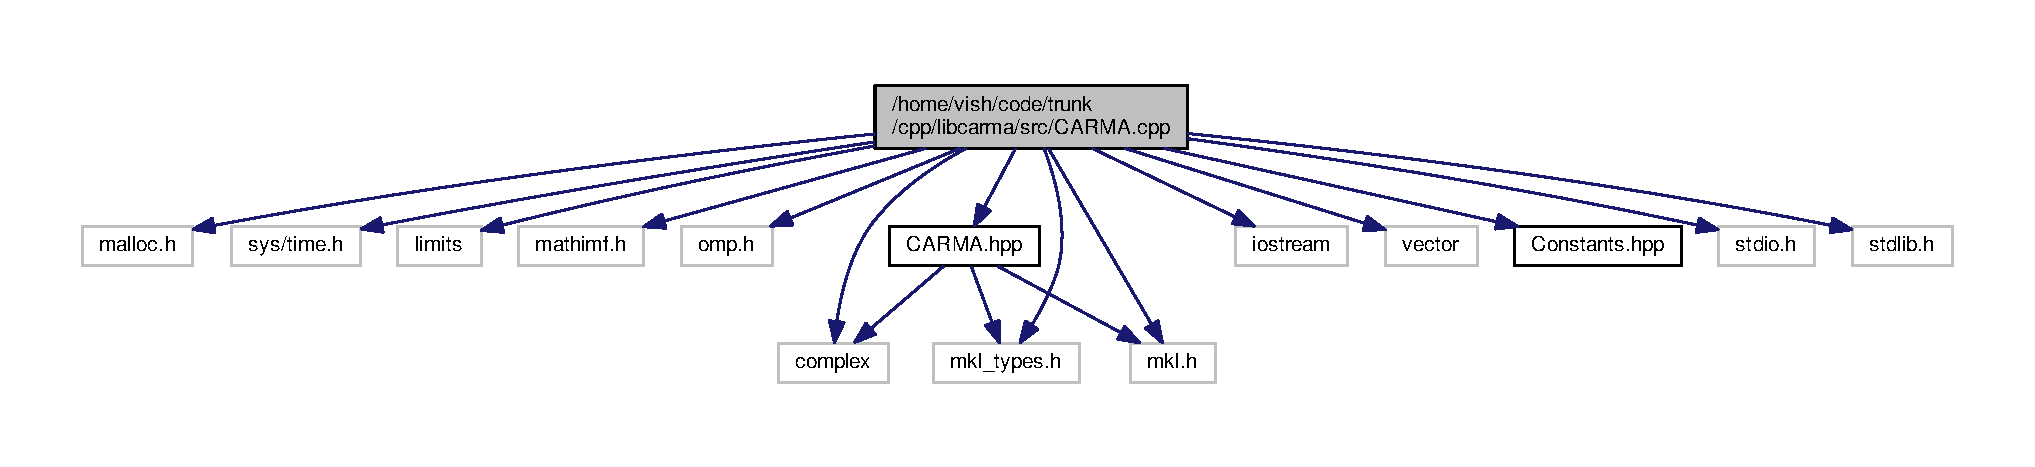
\includegraphics[width=350pt]{_c_a_r_m_a_8cpp__incl}
\end{center}
\end{figure}
\subsection*{Macros}
\begin{DoxyCompactItemize}
\item 
\#define \hyperlink{_c_a_r_m_a_8cpp_a0b45f62ef34311fdb79b8de82d75c0d3}{M\-K\-L\-\_\-\-Complex8}~std\-::complex$<$float$>$
\item 
\#define \hyperlink{_c_a_r_m_a_8cpp_a1fa119034fee07a6d5449926cbb7915a}{M\-K\-L\-\_\-\-Complex16}~std\-::complex$<$double$>$
\end{DoxyCompactItemize}
\subsection*{Functions}
\begin{DoxyCompactItemize}
\item 
double \hyperlink{_c_a_r_m_a_8cpp_a9dd80aa78622e42e58063971be13e31d}{calc\-C\-A\-R\-M\-A\-Ln\-Like} (const vector$<$ double $>$ \&x, vector$<$ double $>$ \&grad, void $\ast$p2\-Args)
\item 
double \hyperlink{_c_a_r_m_a_8cpp_ac36b5c2337263314018956fe8ba6e576}{calc\-C\-A\-R\-M\-A\-Ln\-Like} (double $\ast$walker\-Pos, void $\ast$func\-\_\-args)
\item 
double \hyperlink{_c_a_r_m_a_8cpp_ac6c51cd6959e4a7a5ec0557af951daaa}{calc\-Ln\-Like} (const vector$<$ double $>$ \&x, vector$<$ double $>$ \&grad, void $\ast$p2\-Args)
\item 
double \hyperlink{_c_a_r_m_a_8cpp_af9281261b466e28c15b702652226c5ed}{calc\-Ln\-Like} (double $\ast$walker\-Pos, void $\ast$func\-\_\-args)
\item 
void \hyperlink{_c_a_r_m_a_8cpp_a52e65b8de02410a2382d1c0858c43b25}{zero\-Matrix} (int n\-Rows, int n\-Cols, int $\ast$mat)
\item 
void \hyperlink{_c_a_r_m_a_8cpp_ad06e01d494041ea73f3fb05d5208765f}{zero\-Matrix} (int n\-Rows, int n\-Cols, lapack\-\_\-int $\ast$mat)
\item 
void \hyperlink{_c_a_r_m_a_8cpp_acbdde1f5b60f8f09a2561e877f8279e5}{zero\-Matrix} (int n\-Rows, int n\-Cols, double $\ast$mat)
\item 
void \hyperlink{_c_a_r_m_a_8cpp_aff867598dfd07c509cec6da77c33fb98}{zero\-Matrix} (int n\-Rows, int n\-Cols, complex$<$ double $>$ $\ast$mat)
\item 
void \hyperlink{_c_a_r_m_a_8cpp_adaf529b8047fb0aa639f2aa494b9cfaf}{view\-Matrix} (int n\-Rows, int n\-Cols, double $\ast$mat)
\item 
void \hyperlink{_c_a_r_m_a_8cpp_ab43c14961907b75c90cee7b7fd28a3cc}{view\-Matrix} (int n\-Rows, int n\-Cols, complex$<$ double $>$ $\ast$mat)
\item 
double \hyperlink{_c_a_r_m_a_8cpp_a7a7718261954382ab26f32dae64bf3f4}{dtime} ()
\item 
void \hyperlink{_c_a_r_m_a_8cpp_a0644b006a49b595cc3e4d9cf6dff7303}{kron} (int m, int n, double $\ast$A, int p, int q, double $\ast$B, double $\ast$C)
\end{DoxyCompactItemize}


\subsection{Macro Definition Documentation}
\hypertarget{_c_a_r_m_a_8cpp_a1fa119034fee07a6d5449926cbb7915a}{\index{C\-A\-R\-M\-A.\-cpp@{C\-A\-R\-M\-A.\-cpp}!M\-K\-L\-\_\-\-Complex16@{M\-K\-L\-\_\-\-Complex16}}
\index{M\-K\-L\-\_\-\-Complex16@{M\-K\-L\-\_\-\-Complex16}!CARMA.cpp@{C\-A\-R\-M\-A.\-cpp}}
\subsubsection[{M\-K\-L\-\_\-\-Complex16}]{\setlength{\rightskip}{0pt plus 5cm}\#define M\-K\-L\-\_\-\-Complex16~std\-::complex$<$double$>$}}\label{_c_a_r_m_a_8cpp_a1fa119034fee07a6d5449926cbb7915a}


Definition at line 9 of file C\-A\-R\-M\-A.\-cpp.

\hypertarget{_c_a_r_m_a_8cpp_a0b45f62ef34311fdb79b8de82d75c0d3}{\index{C\-A\-R\-M\-A.\-cpp@{C\-A\-R\-M\-A.\-cpp}!M\-K\-L\-\_\-\-Complex8@{M\-K\-L\-\_\-\-Complex8}}
\index{M\-K\-L\-\_\-\-Complex8@{M\-K\-L\-\_\-\-Complex8}!CARMA.cpp@{C\-A\-R\-M\-A.\-cpp}}
\subsubsection[{M\-K\-L\-\_\-\-Complex8}]{\setlength{\rightskip}{0pt plus 5cm}\#define M\-K\-L\-\_\-\-Complex8~std\-::complex$<$float$>$}}\label{_c_a_r_m_a_8cpp_a0b45f62ef34311fdb79b8de82d75c0d3}


Definition at line 8 of file C\-A\-R\-M\-A.\-cpp.



\subsection{Function Documentation}
\hypertarget{_c_a_r_m_a_8cpp_a9dd80aa78622e42e58063971be13e31d}{\index{C\-A\-R\-M\-A.\-cpp@{C\-A\-R\-M\-A.\-cpp}!calc\-C\-A\-R\-M\-A\-Ln\-Like@{calc\-C\-A\-R\-M\-A\-Ln\-Like}}
\index{calc\-C\-A\-R\-M\-A\-Ln\-Like@{calc\-C\-A\-R\-M\-A\-Ln\-Like}!CARMA.cpp@{C\-A\-R\-M\-A.\-cpp}}
\subsubsection[{calc\-C\-A\-R\-M\-A\-Ln\-Like}]{\setlength{\rightskip}{0pt plus 5cm}double calc\-C\-A\-R\-M\-A\-Ln\-Like (
\begin{DoxyParamCaption}
\item[{const vector$<$ double $>$ \&}]{x, }
\item[{vector$<$ double $>$ \&}]{grad, }
\item[{void $\ast$}]{p2\-Args}
\end{DoxyParamCaption}
)}}\label{_c_a_r_m_a_8cpp_a9dd80aa78622e42e58063971be13e31d}


Definition at line 43 of file C\-A\-R\-M\-A.\-cpp.

\hypertarget{_c_a_r_m_a_8cpp_ac36b5c2337263314018956fe8ba6e576}{\index{C\-A\-R\-M\-A.\-cpp@{C\-A\-R\-M\-A.\-cpp}!calc\-C\-A\-R\-M\-A\-Ln\-Like@{calc\-C\-A\-R\-M\-A\-Ln\-Like}}
\index{calc\-C\-A\-R\-M\-A\-Ln\-Like@{calc\-C\-A\-R\-M\-A\-Ln\-Like}!CARMA.cpp@{C\-A\-R\-M\-A.\-cpp}}
\subsubsection[{calc\-C\-A\-R\-M\-A\-Ln\-Like}]{\setlength{\rightskip}{0pt plus 5cm}double calc\-C\-A\-R\-M\-A\-Ln\-Like (
\begin{DoxyParamCaption}
\item[{double $\ast$}]{walker\-Pos, }
\item[{void $\ast$}]{func\-\_\-args}
\end{DoxyParamCaption}
)}}\label{_c_a_r_m_a_8cpp_ac36b5c2337263314018956fe8ba6e576}


Definition at line 100 of file C\-A\-R\-M\-A.\-cpp.

\hypertarget{_c_a_r_m_a_8cpp_ac6c51cd6959e4a7a5ec0557af951daaa}{\index{C\-A\-R\-M\-A.\-cpp@{C\-A\-R\-M\-A.\-cpp}!calc\-Ln\-Like@{calc\-Ln\-Like}}
\index{calc\-Ln\-Like@{calc\-Ln\-Like}!CARMA.cpp@{C\-A\-R\-M\-A.\-cpp}}
\subsubsection[{calc\-Ln\-Like}]{\setlength{\rightskip}{0pt plus 5cm}double calc\-Ln\-Like (
\begin{DoxyParamCaption}
\item[{const vector$<$ double $>$ \&}]{x, }
\item[{vector$<$ double $>$ \&}]{grad, }
\item[{void $\ast$}]{p2\-Args}
\end{DoxyParamCaption}
)}}\label{_c_a_r_m_a_8cpp_ac6c51cd6959e4a7a5ec0557af951daaa}


Definition at line 151 of file C\-A\-R\-M\-A.\-cpp.



Here is the caller graph for this function\-:\nopagebreak
\begin{figure}[H]
\begin{center}
\leavevmode
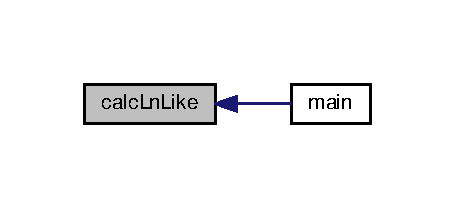
\includegraphics[width=218pt]{_c_a_r_m_a_8cpp_ac6c51cd6959e4a7a5ec0557af951daaa_icgraph}
\end{center}
\end{figure}


\hypertarget{_c_a_r_m_a_8cpp_af9281261b466e28c15b702652226c5ed}{\index{C\-A\-R\-M\-A.\-cpp@{C\-A\-R\-M\-A.\-cpp}!calc\-Ln\-Like@{calc\-Ln\-Like}}
\index{calc\-Ln\-Like@{calc\-Ln\-Like}!CARMA.cpp@{C\-A\-R\-M\-A.\-cpp}}
\subsubsection[{calc\-Ln\-Like}]{\setlength{\rightskip}{0pt plus 5cm}double calc\-Ln\-Like (
\begin{DoxyParamCaption}
\item[{double $\ast$}]{walker\-Pos, }
\item[{void $\ast$}]{func\-\_\-args}
\end{DoxyParamCaption}
)}}\label{_c_a_r_m_a_8cpp_af9281261b466e28c15b702652226c5ed}


Definition at line 208 of file C\-A\-R\-M\-A.\-cpp.

\hypertarget{_c_a_r_m_a_8cpp_a7a7718261954382ab26f32dae64bf3f4}{\index{C\-A\-R\-M\-A.\-cpp@{C\-A\-R\-M\-A.\-cpp}!dtime@{dtime}}
\index{dtime@{dtime}!CARMA.cpp@{C\-A\-R\-M\-A.\-cpp}}
\subsubsection[{dtime}]{\setlength{\rightskip}{0pt plus 5cm}double dtime (
\begin{DoxyParamCaption}
{}
\end{DoxyParamCaption}
)}}\label{_c_a_r_m_a_8cpp_a7a7718261954382ab26f32dae64bf3f4}


Definition at line 318 of file C\-A\-R\-M\-A.\-cpp.



Here is the caller graph for this function\-:\nopagebreak
\begin{figure}[H]
\begin{center}
\leavevmode
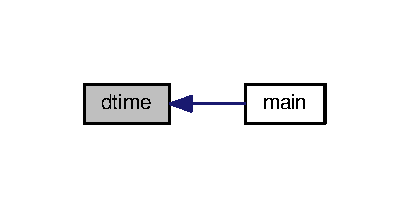
\includegraphics[width=196pt]{_c_a_r_m_a_8cpp_a7a7718261954382ab26f32dae64bf3f4_icgraph}
\end{center}
\end{figure}


\hypertarget{_c_a_r_m_a_8cpp_a0644b006a49b595cc3e4d9cf6dff7303}{\index{C\-A\-R\-M\-A.\-cpp@{C\-A\-R\-M\-A.\-cpp}!kron@{kron}}
\index{kron@{kron}!CARMA.cpp@{C\-A\-R\-M\-A.\-cpp}}
\subsubsection[{kron}]{\setlength{\rightskip}{0pt plus 5cm}void kron (
\begin{DoxyParamCaption}
\item[{int}]{m, }
\item[{int}]{n, }
\item[{double $\ast$}]{A, }
\item[{int}]{p, }
\item[{int}]{q, }
\item[{double $\ast$}]{B, }
\item[{double $\ast$}]{C}
\end{DoxyParamCaption}
)}}\label{_c_a_r_m_a_8cpp_a0644b006a49b595cc3e4d9cf6dff7303}


Definition at line 326 of file C\-A\-R\-M\-A.\-cpp.



Here is the caller graph for this function\-:\nopagebreak
\begin{figure}[H]
\begin{center}
\leavevmode
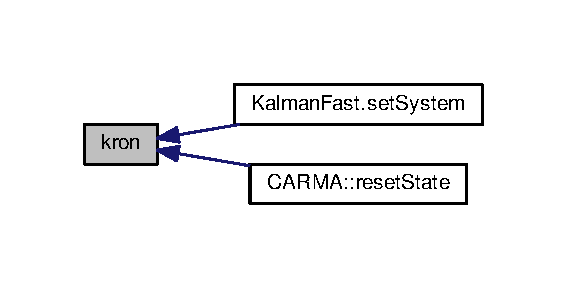
\includegraphics[width=272pt]{_c_a_r_m_a_8cpp_a0644b006a49b595cc3e4d9cf6dff7303_icgraph}
\end{center}
\end{figure}


\hypertarget{_c_a_r_m_a_8cpp_adaf529b8047fb0aa639f2aa494b9cfaf}{\index{C\-A\-R\-M\-A.\-cpp@{C\-A\-R\-M\-A.\-cpp}!view\-Matrix@{view\-Matrix}}
\index{view\-Matrix@{view\-Matrix}!CARMA.cpp@{C\-A\-R\-M\-A.\-cpp}}
\subsubsection[{view\-Matrix}]{\setlength{\rightskip}{0pt plus 5cm}void view\-Matrix (
\begin{DoxyParamCaption}
\item[{int}]{n\-Rows, }
\item[{int}]{n\-Cols, }
\item[{double $\ast$}]{mat}
\end{DoxyParamCaption}
)}}\label{_c_a_r_m_a_8cpp_adaf529b8047fb0aa639f2aa494b9cfaf}


Definition at line 300 of file C\-A\-R\-M\-A.\-cpp.



Here is the caller graph for this function\-:\nopagebreak
\begin{figure}[H]
\begin{center}
\leavevmode
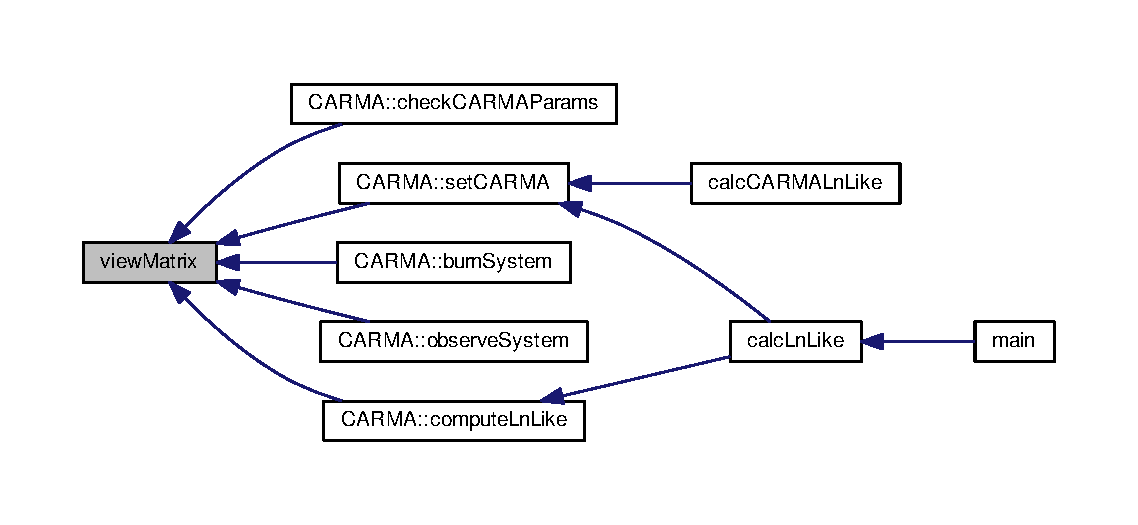
\includegraphics[width=336pt]{_c_a_r_m_a_8cpp_adaf529b8047fb0aa639f2aa494b9cfaf_icgraph}
\end{center}
\end{figure}


\hypertarget{_c_a_r_m_a_8cpp_ab43c14961907b75c90cee7b7fd28a3cc}{\index{C\-A\-R\-M\-A.\-cpp@{C\-A\-R\-M\-A.\-cpp}!view\-Matrix@{view\-Matrix}}
\index{view\-Matrix@{view\-Matrix}!CARMA.cpp@{C\-A\-R\-M\-A.\-cpp}}
\subsubsection[{view\-Matrix}]{\setlength{\rightskip}{0pt plus 5cm}void view\-Matrix (
\begin{DoxyParamCaption}
\item[{int}]{n\-Rows, }
\item[{int}]{n\-Cols, }
\item[{complex$<$ double $>$ $\ast$}]{mat}
\end{DoxyParamCaption}
)}}\label{_c_a_r_m_a_8cpp_ab43c14961907b75c90cee7b7fd28a3cc}


Definition at line 309 of file C\-A\-R\-M\-A.\-cpp.

\hypertarget{_c_a_r_m_a_8cpp_a52e65b8de02410a2382d1c0858c43b25}{\index{C\-A\-R\-M\-A.\-cpp@{C\-A\-R\-M\-A.\-cpp}!zero\-Matrix@{zero\-Matrix}}
\index{zero\-Matrix@{zero\-Matrix}!CARMA.cpp@{C\-A\-R\-M\-A.\-cpp}}
\subsubsection[{zero\-Matrix}]{\setlength{\rightskip}{0pt plus 5cm}void zero\-Matrix (
\begin{DoxyParamCaption}
\item[{int}]{n\-Rows, }
\item[{int}]{n\-Cols, }
\item[{int $\ast$}]{mat}
\end{DoxyParamCaption}
)}}\label{_c_a_r_m_a_8cpp_a52e65b8de02410a2382d1c0858c43b25}


Definition at line 268 of file C\-A\-R\-M\-A.\-cpp.

\hypertarget{_c_a_r_m_a_8cpp_ad06e01d494041ea73f3fb05d5208765f}{\index{C\-A\-R\-M\-A.\-cpp@{C\-A\-R\-M\-A.\-cpp}!zero\-Matrix@{zero\-Matrix}}
\index{zero\-Matrix@{zero\-Matrix}!CARMA.cpp@{C\-A\-R\-M\-A.\-cpp}}
\subsubsection[{zero\-Matrix}]{\setlength{\rightskip}{0pt plus 5cm}void zero\-Matrix (
\begin{DoxyParamCaption}
\item[{int}]{n\-Rows, }
\item[{int}]{n\-Cols, }
\item[{lapack\-\_\-int $\ast$}]{mat}
\end{DoxyParamCaption}
)}}\label{_c_a_r_m_a_8cpp_ad06e01d494041ea73f3fb05d5208765f}


Definition at line 276 of file C\-A\-R\-M\-A.\-cpp.

\hypertarget{_c_a_r_m_a_8cpp_acbdde1f5b60f8f09a2561e877f8279e5}{\index{C\-A\-R\-M\-A.\-cpp@{C\-A\-R\-M\-A.\-cpp}!zero\-Matrix@{zero\-Matrix}}
\index{zero\-Matrix@{zero\-Matrix}!CARMA.cpp@{C\-A\-R\-M\-A.\-cpp}}
\subsubsection[{zero\-Matrix}]{\setlength{\rightskip}{0pt plus 5cm}void zero\-Matrix (
\begin{DoxyParamCaption}
\item[{int}]{n\-Rows, }
\item[{int}]{n\-Cols, }
\item[{double $\ast$}]{mat}
\end{DoxyParamCaption}
)}}\label{_c_a_r_m_a_8cpp_acbdde1f5b60f8f09a2561e877f8279e5}


Definition at line 284 of file C\-A\-R\-M\-A.\-cpp.

\hypertarget{_c_a_r_m_a_8cpp_aff867598dfd07c509cec6da77c33fb98}{\index{C\-A\-R\-M\-A.\-cpp@{C\-A\-R\-M\-A.\-cpp}!zero\-Matrix@{zero\-Matrix}}
\index{zero\-Matrix@{zero\-Matrix}!CARMA.cpp@{C\-A\-R\-M\-A.\-cpp}}
\subsubsection[{zero\-Matrix}]{\setlength{\rightskip}{0pt plus 5cm}void zero\-Matrix (
\begin{DoxyParamCaption}
\item[{int}]{n\-Rows, }
\item[{int}]{n\-Cols, }
\item[{complex$<$ double $>$ $\ast$}]{mat}
\end{DoxyParamCaption}
)}}\label{_c_a_r_m_a_8cpp_aff867598dfd07c509cec6da77c33fb98}


Definition at line 292 of file C\-A\-R\-M\-A.\-cpp.


\hypertarget{_c_a_r_m_a_task_8cpp}{\section{/home/vish/code/trunk/cpp/libcarma/cython/src/\-C\-A\-R\-M\-A\-Task.cpp File Reference}
\label{_c_a_r_m_a_task_8cpp}\index{/home/vish/code/trunk/cpp/libcarma/cython/src/\-C\-A\-R\-M\-A\-Task.\-cpp@{/home/vish/code/trunk/cpp/libcarma/cython/src/\-C\-A\-R\-M\-A\-Task.\-cpp}}
}
{\ttfamily \#include \char`\"{}Python.\-h\char`\"{}}\\*
Include dependency graph for C\-A\-R\-M\-A\-Task.\-cpp\-:
\subsection*{Macros}
\begin{DoxyCompactItemize}
\item 
\#define \hyperlink{_c_a_r_m_a_task_8cpp_ac9efdaac9411d0868b715edccca3269d}{P\-Y\-\_\-\-S\-S\-I\-Z\-E\-\_\-\-T\-\_\-\-C\-L\-E\-A\-N}
\end{DoxyCompactItemize}


\subsection{Macro Definition Documentation}
\hypertarget{_c_a_r_m_a_task_8cpp_ac9efdaac9411d0868b715edccca3269d}{\index{C\-A\-R\-M\-A\-Task.\-cpp@{C\-A\-R\-M\-A\-Task.\-cpp}!P\-Y\-\_\-\-S\-S\-I\-Z\-E\-\_\-\-T\-\_\-\-C\-L\-E\-A\-N@{P\-Y\-\_\-\-S\-S\-I\-Z\-E\-\_\-\-T\-\_\-\-C\-L\-E\-A\-N}}
\index{P\-Y\-\_\-\-S\-S\-I\-Z\-E\-\_\-\-T\-\_\-\-C\-L\-E\-A\-N@{P\-Y\-\_\-\-S\-S\-I\-Z\-E\-\_\-\-T\-\_\-\-C\-L\-E\-A\-N}!CARMATask.cpp@{C\-A\-R\-M\-A\-Task.\-cpp}}
\subsubsection[{P\-Y\-\_\-\-S\-S\-I\-Z\-E\-\_\-\-T\-\_\-\-C\-L\-E\-A\-N}]{\setlength{\rightskip}{0pt plus 5cm}\#define P\-Y\-\_\-\-S\-S\-I\-Z\-E\-\_\-\-T\-\_\-\-C\-L\-E\-A\-N}}\label{_c_a_r_m_a_task_8cpp_ac9efdaac9411d0868b715edccca3269d}


Definition at line 58 of file C\-A\-R\-M\-A\-Task.\-cpp.


\hypertarget{_constants_8cpp}{\section{/home/vish/code/trunk/cpp/libcarma/cython/src/\-Constants.cpp File Reference}
\label{_constants_8cpp}\index{/home/vish/code/trunk/cpp/libcarma/cython/src/\-Constants.\-cpp@{/home/vish/code/trunk/cpp/libcarma/cython/src/\-Constants.\-cpp}}
}
{\ttfamily \#include $<$cmath$>$}\\*
{\ttfamily \#include $<$mathimf.\-h$>$}\\*
{\ttfamily \#include $<$complex$>$}\\*
{\ttfamily \#include \char`\"{}Constants.\-hpp\char`\"{}}\\*
Include dependency graph for Constants.\-cpp\-:
\subsection*{Functions}
\begin{DoxyCompactItemize}
\item 
complex$<$ double $>$ \hyperlink{_constants_8cpp_a60965ce7302347a2e697391416a29cca}{complex\-Zero} (0.\-0, 0.\-0)
\item 
complex$<$ double $>$ \hyperlink{_constants_8cpp_aa8578dabbff8c9dad78c162665c32af8}{complex\-One} (1.\-0, 0.\-0)
\end{DoxyCompactItemize}
\subsection*{Variables}
\begin{DoxyCompactItemize}
\item 
double \hyperlink{_constants_8cpp_a31c17cc321db72d5ab448b71ea92792f}{pi} = 3.\-1415926535897932384626433832795028841971693993751058209749445923078164062862089986280348253421170679
\item 
double \hyperlink{_constants_8cpp_a18bbe41d56bab00212fd0e8e733e9f1f}{pi\-Sq} = pow(\hyperlink{_constants_8cpp_a31c17cc321db72d5ab448b71ea92792f}{pi}, 2.\-0)
\item 
double \hyperlink{_constants_8cpp_ab17e17fb32b792781b807505e7f60c9c}{e} = 2.\-71828182845904523536028747135266249775724709369995
\item 
double \hyperlink{_constants_8cpp_a5ce1018aef28e71271ae3b4431210720}{infinite\-Val} = H\-U\-G\-E\-\_\-\-V\-A\-L
\item 
double \hyperlink{_constants_8cpp_a67783a2c4f670ee5a9dadcf428324d32}{G} = 6.\-67408e-\/11
\item 
double \hyperlink{_constants_8cpp_a2c09e929a6ea340fc9653cca414b11d3}{c} = 299792458.\-0
\item 
double \hyperlink{_constants_8cpp_a8497a2d27908c87901466c9de72ff8d8}{A\-U} = 1.\-4960e11
\item 
double \hyperlink{_constants_8cpp_a2e08042cd1e7eb1861e7115f34fa3acb}{Parsec} = 3.\-0857e16
\item 
double \hyperlink{_constants_8cpp_a187ad5035a30f1230f63152e677791ba}{Day} = 86164.\-090530833
\item 
double \hyperlink{_constants_8cpp_aa2047f98d2c2eecb4bfe0d2bd43ac10e}{Year} = 31557600.\-0
\item 
double \hyperlink{_constants_8cpp_ade81fa2dde12779958f5cafad2d62a6f}{kms} = 1.\-0e3
\item 
double \hyperlink{_constants_8cpp_ada9035453156e0ae346332fde905c274}{Solar\-Mass} = 1.\-98855e30
\item 
double \hyperlink{_constants_8cpp_a798a374e513280a7d37661626aab93d5}{Solar\-Mass\-Per\-Cubic\-Parsec} = \hyperlink{_constants_8cpp_ada9035453156e0ae346332fde905c274}{Solar\-Mass}/pow(\hyperlink{_constants_8cpp_a2e08042cd1e7eb1861e7115f34fa3acb}{Parsec}, 3.\-0)
\item 
double \hyperlink{_constants_8cpp_a6a9e5bbdf108936466078a267b5acd51}{integration\-Time} = 6.\-019802903
\item 
double \hyperlink{_constants_8cpp_abd52f1ed1ece35cffe3fc3e4180ca0f3}{read\-Time} = 0.\-5189485261
\item 
int \hyperlink{_constants_8cpp_aeab23e8ce3743c4e554e657ce55c5305}{num\-Integrations\-S\-C} = 9
\item 
int \hyperlink{_constants_8cpp_a045a70c6ff8d3041c66cb29263a0f815}{num\-Integrations\-L\-C} = 270
\item 
double \hyperlink{_constants_8cpp_a3b68866972010d697c2f9e3def43a8c4}{sampling\-Interval\-S\-C} = (\hyperlink{_constants_8cpp_a6a9e5bbdf108936466078a267b5acd51}{integration\-Time}+\hyperlink{_constants_8cpp_abd52f1ed1ece35cffe3fc3e4180ca0f3}{read\-Time})$\ast$\hyperlink{_constants_8cpp_aeab23e8ce3743c4e554e657ce55c5305}{num\-Integrations\-S\-C}
\item 
double \hyperlink{_constants_8cpp_a7eec0eac1517df1522a3775fc44ddf7d}{sampling\-Interval\-L\-C} = (\hyperlink{_constants_8cpp_a6a9e5bbdf108936466078a267b5acd51}{integration\-Time}+\hyperlink{_constants_8cpp_abd52f1ed1ece35cffe3fc3e4180ca0f3}{read\-Time})$\ast$\hyperlink{_constants_8cpp_a045a70c6ff8d3041c66cb29263a0f815}{num\-Integrations\-L\-C}
\item 
double \hyperlink{_constants_8cpp_abae737372bcd2caafbf77434f3b0ed97}{sampling\-Frequency\-S\-C} = 1.\-0/((\hyperlink{_constants_8cpp_a6a9e5bbdf108936466078a267b5acd51}{integration\-Time}+\hyperlink{_constants_8cpp_abd52f1ed1ece35cffe3fc3e4180ca0f3}{read\-Time})$\ast$\hyperlink{_constants_8cpp_aeab23e8ce3743c4e554e657ce55c5305}{num\-Integrations\-S\-C})
\item 
double \hyperlink{_constants_8cpp_a102f4d453dc44d0a812bde4a0c8c19c8}{sampling\-Frequency\-L\-C} = 1.\-0/((\hyperlink{_constants_8cpp_a6a9e5bbdf108936466078a267b5acd51}{integration\-Time}+\hyperlink{_constants_8cpp_abd52f1ed1ece35cffe3fc3e4180ca0f3}{read\-Time})$\ast$\hyperlink{_constants_8cpp_a045a70c6ff8d3041c66cb29263a0f815}{num\-Integrations\-L\-C})
\item 
double \hyperlink{_constants_8cpp_a29c58ec25452277c1661f674327a77a4}{Nyquist\-Frequency\-S\-C} = \hyperlink{_constants_8cpp_abae737372bcd2caafbf77434f3b0ed97}{sampling\-Frequency\-S\-C}/2.\-0
\item 
double \hyperlink{_constants_8cpp_a598be37cc4a0d559305212b7e8c21045}{Nyquist\-Frequency\-L\-C} = \hyperlink{_constants_8cpp_a102f4d453dc44d0a812bde4a0c8c19c8}{sampling\-Frequency\-L\-C}/2.\-0
\item 
double \hyperlink{_constants_8cpp_ad273a878a46f52a8c720ef7eae03ae4f}{sec\-Per\-Sidereal\-Day} = 86164.\-090530833
\item 
double \hyperlink{_constants_8cpp_ad55d7bc1d7b5c686f6197b02498e4eaf}{sc\-Cadence} = (\hyperlink{_constants_8cpp_a6a9e5bbdf108936466078a267b5acd51}{integration\-Time}+\hyperlink{_constants_8cpp_abd52f1ed1ece35cffe3fc3e4180ca0f3}{read\-Time})$\ast$\hyperlink{_constants_8cpp_aeab23e8ce3743c4e554e657ce55c5305}{num\-Integrations\-S\-C}
\item 
double \hyperlink{_constants_8cpp_ac18142dbc207474c073432f4b28424b9}{lc\-Cadence} = (\hyperlink{_constants_8cpp_a6a9e5bbdf108936466078a267b5acd51}{integration\-Time}+\hyperlink{_constants_8cpp_abd52f1ed1ece35cffe3fc3e4180ca0f3}{read\-Time})$\ast$\hyperlink{_constants_8cpp_a045a70c6ff8d3041c66cb29263a0f815}{num\-Integrations\-L\-C}
\item 
double \hyperlink{_constants_8cpp_a6a5210c2bcb5149c1073568e5c8d6599}{log2\-Of\-E} = log2(\hyperlink{_constants_8cpp_ab17e17fb32b792781b807505e7f60c9c}{e})
\item 
double \hyperlink{_constants_8cpp_a2b27190acf3cc471e389bb8173544658}{log2\-Pi} = log2(2.\-0$\ast$\hyperlink{_constants_8cpp_a31c17cc321db72d5ab448b71ea92792f}{pi})/\hyperlink{_constants_8cpp_a6a5210c2bcb5149c1073568e5c8d6599}{log2\-Of\-E}
\end{DoxyCompactItemize}


\subsection{Function Documentation}
\hypertarget{_constants_8cpp_aa8578dabbff8c9dad78c162665c32af8}{\index{Constants.\-cpp@{Constants.\-cpp}!complex\-One@{complex\-One}}
\index{complex\-One@{complex\-One}!Constants.cpp@{Constants.\-cpp}}
\subsubsection[{complex\-One}]{\setlength{\rightskip}{0pt plus 5cm}complex$<$double$>$ complex\-One (
\begin{DoxyParamCaption}
\item[{1.}]{0, }
\item[{0.}]{0}
\end{DoxyParamCaption}
)}}\label{_constants_8cpp_aa8578dabbff8c9dad78c162665c32af8}
\hypertarget{_constants_8cpp_a60965ce7302347a2e697391416a29cca}{\index{Constants.\-cpp@{Constants.\-cpp}!complex\-Zero@{complex\-Zero}}
\index{complex\-Zero@{complex\-Zero}!Constants.cpp@{Constants.\-cpp}}
\subsubsection[{complex\-Zero}]{\setlength{\rightskip}{0pt plus 5cm}complex$<$double$>$ complex\-Zero (
\begin{DoxyParamCaption}
\item[{0.}]{0, }
\item[{0.}]{0}
\end{DoxyParamCaption}
)}}\label{_constants_8cpp_a60965ce7302347a2e697391416a29cca}


\subsection{Variable Documentation}
\hypertarget{_constants_8cpp_a8497a2d27908c87901466c9de72ff8d8}{\index{Constants.\-cpp@{Constants.\-cpp}!A\-U@{A\-U}}
\index{A\-U@{A\-U}!Constants.cpp@{Constants.\-cpp}}
\subsubsection[{A\-U}]{\setlength{\rightskip}{0pt plus 5cm}double A\-U = 1.\-4960e11}}\label{_constants_8cpp_a8497a2d27908c87901466c9de72ff8d8}


Definition at line 27 of file binary\-S\-M\-B\-H\-Demo.\-py.

\hypertarget{_constants_8cpp_a2c09e929a6ea340fc9653cca414b11d3}{\index{Constants.\-cpp@{Constants.\-cpp}!c@{c}}
\index{c@{c}!Constants.cpp@{Constants.\-cpp}}
\subsubsection[{c}]{\setlength{\rightskip}{0pt plus 5cm}double c = 299792458.\-0}}\label{_constants_8cpp_a2c09e929a6ea340fc9653cca414b11d3}


Definition at line 26 of file binary\-S\-M\-B\-H\-Demo.\-py.

\hypertarget{_constants_8cpp_a187ad5035a30f1230f63152e677791ba}{\index{Constants.\-cpp@{Constants.\-cpp}!Day@{Day}}
\index{Day@{Day}!Constants.cpp@{Constants.\-cpp}}
\subsubsection[{Day}]{\setlength{\rightskip}{0pt plus 5cm}double Day = 86164.\-090530833}}\label{_constants_8cpp_a187ad5035a30f1230f63152e677791ba}


Definition at line 30 of file binary\-S\-M\-B\-H\-Demo.\-py.

\hypertarget{_constants_8cpp_ab17e17fb32b792781b807505e7f60c9c}{\index{Constants.\-cpp@{Constants.\-cpp}!e@{e}}
\index{e@{e}!Constants.cpp@{Constants.\-cpp}}
\subsubsection[{e}]{\setlength{\rightskip}{0pt plus 5cm}double e = 2.\-71828182845904523536028747135266249775724709369995}}\label{_constants_8cpp_ab17e17fb32b792781b807505e7f60c9c}
\hypertarget{_constants_8cpp_a67783a2c4f670ee5a9dadcf428324d32}{\index{Constants.\-cpp@{Constants.\-cpp}!G@{G}}
\index{G@{G}!Constants.cpp@{Constants.\-cpp}}
\subsubsection[{G}]{\setlength{\rightskip}{0pt plus 5cm}double G = 6.\-67408e-\/11}}\label{_constants_8cpp_a67783a2c4f670ee5a9dadcf428324d32}


Definition at line 25 of file binary\-S\-M\-B\-H\-Demo.\-py.

\hypertarget{_constants_8cpp_a5ce1018aef28e71271ae3b4431210720}{\index{Constants.\-cpp@{Constants.\-cpp}!infinite\-Val@{infinite\-Val}}
\index{infinite\-Val@{infinite\-Val}!Constants.cpp@{Constants.\-cpp}}
\subsubsection[{infinite\-Val}]{\setlength{\rightskip}{0pt plus 5cm}double infinite\-Val = H\-U\-G\-E\-\_\-\-V\-A\-L}}\label{_constants_8cpp_a5ce1018aef28e71271ae3b4431210720}
\hypertarget{_constants_8cpp_a6a9e5bbdf108936466078a267b5acd51}{\index{Constants.\-cpp@{Constants.\-cpp}!integration\-Time@{integration\-Time}}
\index{integration\-Time@{integration\-Time}!Constants.cpp@{Constants.\-cpp}}
\subsubsection[{integration\-Time}]{\setlength{\rightskip}{0pt plus 5cm}double integration\-Time = 6.\-019802903}}\label{_constants_8cpp_a6a9e5bbdf108936466078a267b5acd51}
\hypertarget{_constants_8cpp_ade81fa2dde12779958f5cafad2d62a6f}{\index{Constants.\-cpp@{Constants.\-cpp}!kms@{kms}}
\index{kms@{kms}!Constants.cpp@{Constants.\-cpp}}
\subsubsection[{kms}]{\setlength{\rightskip}{0pt plus 5cm}double kms = 1.\-0e3}}\label{_constants_8cpp_ade81fa2dde12779958f5cafad2d62a6f}
\hypertarget{_constants_8cpp_ac18142dbc207474c073432f4b28424b9}{\index{Constants.\-cpp@{Constants.\-cpp}!lc\-Cadence@{lc\-Cadence}}
\index{lc\-Cadence@{lc\-Cadence}!Constants.cpp@{Constants.\-cpp}}
\subsubsection[{lc\-Cadence}]{\setlength{\rightskip}{0pt plus 5cm}double lc\-Cadence = ({\bf integration\-Time}+{\bf read\-Time})$\ast${\bf num\-Integrations\-L\-C}}}\label{_constants_8cpp_ac18142dbc207474c073432f4b28424b9}
\hypertarget{_constants_8cpp_a6a5210c2bcb5149c1073568e5c8d6599}{\index{Constants.\-cpp@{Constants.\-cpp}!log2\-Of\-E@{log2\-Of\-E}}
\index{log2\-Of\-E@{log2\-Of\-E}!Constants.cpp@{Constants.\-cpp}}
\subsubsection[{log2\-Of\-E}]{\setlength{\rightskip}{0pt plus 5cm}double log2\-Of\-E = log2({\bf e})}}\label{_constants_8cpp_a6a5210c2bcb5149c1073568e5c8d6599}
\hypertarget{_constants_8cpp_a2b27190acf3cc471e389bb8173544658}{\index{Constants.\-cpp@{Constants.\-cpp}!log2\-Pi@{log2\-Pi}}
\index{log2\-Pi@{log2\-Pi}!Constants.cpp@{Constants.\-cpp}}
\subsubsection[{log2\-Pi}]{\setlength{\rightskip}{0pt plus 5cm}double log2\-Pi = log2(2.\-0$\ast${\bf pi})/{\bf log2\-Of\-E}}}\label{_constants_8cpp_a2b27190acf3cc471e389bb8173544658}
\hypertarget{_constants_8cpp_a045a70c6ff8d3041c66cb29263a0f815}{\index{Constants.\-cpp@{Constants.\-cpp}!num\-Integrations\-L\-C@{num\-Integrations\-L\-C}}
\index{num\-Integrations\-L\-C@{num\-Integrations\-L\-C}!Constants.cpp@{Constants.\-cpp}}
\subsubsection[{num\-Integrations\-L\-C}]{\setlength{\rightskip}{0pt plus 5cm}int num\-Integrations\-L\-C = 270}}\label{_constants_8cpp_a045a70c6ff8d3041c66cb29263a0f815}
\hypertarget{_constants_8cpp_aeab23e8ce3743c4e554e657ce55c5305}{\index{Constants.\-cpp@{Constants.\-cpp}!num\-Integrations\-S\-C@{num\-Integrations\-S\-C}}
\index{num\-Integrations\-S\-C@{num\-Integrations\-S\-C}!Constants.cpp@{Constants.\-cpp}}
\subsubsection[{num\-Integrations\-S\-C}]{\setlength{\rightskip}{0pt plus 5cm}int num\-Integrations\-S\-C = 9}}\label{_constants_8cpp_aeab23e8ce3743c4e554e657ce55c5305}
\hypertarget{_constants_8cpp_a598be37cc4a0d559305212b7e8c21045}{\index{Constants.\-cpp@{Constants.\-cpp}!Nyquist\-Frequency\-L\-C@{Nyquist\-Frequency\-L\-C}}
\index{Nyquist\-Frequency\-L\-C@{Nyquist\-Frequency\-L\-C}!Constants.cpp@{Constants.\-cpp}}
\subsubsection[{Nyquist\-Frequency\-L\-C}]{\setlength{\rightskip}{0pt plus 5cm}double Nyquist\-Frequency\-L\-C = {\bf sampling\-Frequency\-L\-C}/2.\-0}}\label{_constants_8cpp_a598be37cc4a0d559305212b7e8c21045}
\hypertarget{_constants_8cpp_a29c58ec25452277c1661f674327a77a4}{\index{Constants.\-cpp@{Constants.\-cpp}!Nyquist\-Frequency\-S\-C@{Nyquist\-Frequency\-S\-C}}
\index{Nyquist\-Frequency\-S\-C@{Nyquist\-Frequency\-S\-C}!Constants.cpp@{Constants.\-cpp}}
\subsubsection[{Nyquist\-Frequency\-S\-C}]{\setlength{\rightskip}{0pt plus 5cm}double Nyquist\-Frequency\-S\-C = {\bf sampling\-Frequency\-S\-C}/2.\-0}}\label{_constants_8cpp_a29c58ec25452277c1661f674327a77a4}
\hypertarget{_constants_8cpp_a2e08042cd1e7eb1861e7115f34fa3acb}{\index{Constants.\-cpp@{Constants.\-cpp}!Parsec@{Parsec}}
\index{Parsec@{Parsec}!Constants.cpp@{Constants.\-cpp}}
\subsubsection[{Parsec}]{\setlength{\rightskip}{0pt plus 5cm}double Parsec = 3.\-0857e16}}\label{_constants_8cpp_a2e08042cd1e7eb1861e7115f34fa3acb}


Definition at line 28 of file binary\-S\-M\-B\-H\-Demo.\-py.

\hypertarget{_constants_8cpp_a31c17cc321db72d5ab448b71ea92792f}{\index{Constants.\-cpp@{Constants.\-cpp}!pi@{pi}}
\index{pi@{pi}!Constants.cpp@{Constants.\-cpp}}
\subsubsection[{pi}]{\setlength{\rightskip}{0pt plus 5cm}double pi = 3.\-1415926535897932384626433832795028841971693993751058209749445923078164062862089986280348253421170679}}\label{_constants_8cpp_a31c17cc321db72d5ab448b71ea92792f}
\hypertarget{_constants_8cpp_a18bbe41d56bab00212fd0e8e733e9f1f}{\index{Constants.\-cpp@{Constants.\-cpp}!pi\-Sq@{pi\-Sq}}
\index{pi\-Sq@{pi\-Sq}!Constants.cpp@{Constants.\-cpp}}
\subsubsection[{pi\-Sq}]{\setlength{\rightskip}{0pt plus 5cm}double pi\-Sq = pow({\bf pi}, 2.\-0)}}\label{_constants_8cpp_a18bbe41d56bab00212fd0e8e733e9f1f}
\hypertarget{_constants_8cpp_abd52f1ed1ece35cffe3fc3e4180ca0f3}{\index{Constants.\-cpp@{Constants.\-cpp}!read\-Time@{read\-Time}}
\index{read\-Time@{read\-Time}!Constants.cpp@{Constants.\-cpp}}
\subsubsection[{read\-Time}]{\setlength{\rightskip}{0pt plus 5cm}double read\-Time = 0.\-5189485261}}\label{_constants_8cpp_abd52f1ed1ece35cffe3fc3e4180ca0f3}
\hypertarget{_constants_8cpp_a102f4d453dc44d0a812bde4a0c8c19c8}{\index{Constants.\-cpp@{Constants.\-cpp}!sampling\-Frequency\-L\-C@{sampling\-Frequency\-L\-C}}
\index{sampling\-Frequency\-L\-C@{sampling\-Frequency\-L\-C}!Constants.cpp@{Constants.\-cpp}}
\subsubsection[{sampling\-Frequency\-L\-C}]{\setlength{\rightskip}{0pt plus 5cm}double sampling\-Frequency\-L\-C = 1.\-0/(({\bf integration\-Time}+{\bf read\-Time})$\ast${\bf num\-Integrations\-L\-C})}}\label{_constants_8cpp_a102f4d453dc44d0a812bde4a0c8c19c8}
\hypertarget{_constants_8cpp_abae737372bcd2caafbf77434f3b0ed97}{\index{Constants.\-cpp@{Constants.\-cpp}!sampling\-Frequency\-S\-C@{sampling\-Frequency\-S\-C}}
\index{sampling\-Frequency\-S\-C@{sampling\-Frequency\-S\-C}!Constants.cpp@{Constants.\-cpp}}
\subsubsection[{sampling\-Frequency\-S\-C}]{\setlength{\rightskip}{0pt plus 5cm}double sampling\-Frequency\-S\-C = 1.\-0/(({\bf integration\-Time}+{\bf read\-Time})$\ast${\bf num\-Integrations\-S\-C})}}\label{_constants_8cpp_abae737372bcd2caafbf77434f3b0ed97}
\hypertarget{_constants_8cpp_a7eec0eac1517df1522a3775fc44ddf7d}{\index{Constants.\-cpp@{Constants.\-cpp}!sampling\-Interval\-L\-C@{sampling\-Interval\-L\-C}}
\index{sampling\-Interval\-L\-C@{sampling\-Interval\-L\-C}!Constants.cpp@{Constants.\-cpp}}
\subsubsection[{sampling\-Interval\-L\-C}]{\setlength{\rightskip}{0pt plus 5cm}double sampling\-Interval\-L\-C = ({\bf integration\-Time}+{\bf read\-Time})$\ast${\bf num\-Integrations\-L\-C}}}\label{_constants_8cpp_a7eec0eac1517df1522a3775fc44ddf7d}
\hypertarget{_constants_8cpp_a3b68866972010d697c2f9e3def43a8c4}{\index{Constants.\-cpp@{Constants.\-cpp}!sampling\-Interval\-S\-C@{sampling\-Interval\-S\-C}}
\index{sampling\-Interval\-S\-C@{sampling\-Interval\-S\-C}!Constants.cpp@{Constants.\-cpp}}
\subsubsection[{sampling\-Interval\-S\-C}]{\setlength{\rightskip}{0pt plus 5cm}double sampling\-Interval\-S\-C = ({\bf integration\-Time}+{\bf read\-Time})$\ast${\bf num\-Integrations\-S\-C}}}\label{_constants_8cpp_a3b68866972010d697c2f9e3def43a8c4}
\hypertarget{_constants_8cpp_ad55d7bc1d7b5c686f6197b02498e4eaf}{\index{Constants.\-cpp@{Constants.\-cpp}!sc\-Cadence@{sc\-Cadence}}
\index{sc\-Cadence@{sc\-Cadence}!Constants.cpp@{Constants.\-cpp}}
\subsubsection[{sc\-Cadence}]{\setlength{\rightskip}{0pt plus 5cm}double sc\-Cadence = ({\bf integration\-Time}+{\bf read\-Time})$\ast${\bf num\-Integrations\-S\-C}}}\label{_constants_8cpp_ad55d7bc1d7b5c686f6197b02498e4eaf}
\hypertarget{_constants_8cpp_ad273a878a46f52a8c720ef7eae03ae4f}{\index{Constants.\-cpp@{Constants.\-cpp}!sec\-Per\-Sidereal\-Day@{sec\-Per\-Sidereal\-Day}}
\index{sec\-Per\-Sidereal\-Day@{sec\-Per\-Sidereal\-Day}!Constants.cpp@{Constants.\-cpp}}
\subsubsection[{sec\-Per\-Sidereal\-Day}]{\setlength{\rightskip}{0pt plus 5cm}double sec\-Per\-Sidereal\-Day = 86164.\-090530833}}\label{_constants_8cpp_ad273a878a46f52a8c720ef7eae03ae4f}
\hypertarget{_constants_8cpp_ada9035453156e0ae346332fde905c274}{\index{Constants.\-cpp@{Constants.\-cpp}!Solar\-Mass@{Solar\-Mass}}
\index{Solar\-Mass@{Solar\-Mass}!Constants.cpp@{Constants.\-cpp}}
\subsubsection[{Solar\-Mass}]{\setlength{\rightskip}{0pt plus 5cm}double Solar\-Mass = 1.\-98855e30}}\label{_constants_8cpp_ada9035453156e0ae346332fde905c274}


Definition at line 32 of file binary\-S\-M\-B\-H\-Demo.\-py.

\hypertarget{_constants_8cpp_a798a374e513280a7d37661626aab93d5}{\index{Constants.\-cpp@{Constants.\-cpp}!Solar\-Mass\-Per\-Cubic\-Parsec@{Solar\-Mass\-Per\-Cubic\-Parsec}}
\index{Solar\-Mass\-Per\-Cubic\-Parsec@{Solar\-Mass\-Per\-Cubic\-Parsec}!Constants.cpp@{Constants.\-cpp}}
\subsubsection[{Solar\-Mass\-Per\-Cubic\-Parsec}]{\setlength{\rightskip}{0pt plus 5cm}double Solar\-Mass\-Per\-Cubic\-Parsec = {\bf Solar\-Mass}/pow({\bf Parsec}, 3.\-0)}}\label{_constants_8cpp_a798a374e513280a7d37661626aab93d5}


Definition at line 34 of file binary\-S\-M\-B\-H\-Demo.\-py.

\hypertarget{_constants_8cpp_aa2047f98d2c2eecb4bfe0d2bd43ac10e}{\index{Constants.\-cpp@{Constants.\-cpp}!Year@{Year}}
\index{Year@{Year}!Constants.cpp@{Constants.\-cpp}}
\subsubsection[{Year}]{\setlength{\rightskip}{0pt plus 5cm}double Year = 31557600.\-0}}\label{_constants_8cpp_aa2047f98d2c2eecb4bfe0d2bd43ac10e}


Definition at line 29 of file binary\-S\-M\-B\-H\-Demo.\-py.


\hypertarget{_l_c_8cpp}{\section{/home/vish/code/trunk/cpp/libcarma/cython/src/\-L\-C.cpp File Reference}
\label{_l_c_8cpp}\index{/home/vish/code/trunk/cpp/libcarma/cython/src/\-L\-C.\-cpp@{/home/vish/code/trunk/cpp/libcarma/cython/src/\-L\-C.\-cpp}}
}
{\ttfamily \#include $<$mathimf.\-h$>$}\\*
{\ttfamily \#include $<$complex$>$}\\*
{\ttfamily \#include $<$mkl.\-h$>$}\\*
{\ttfamily \#include $<$mkl\-\_\-types.\-h$>$}\\*
{\ttfamily \#include $<$omp.\-h$>$}\\*
{\ttfamily \#include $<$limits$>$}\\*
{\ttfamily \#include \char`\"{}L\-C.\-hpp\char`\"{}}\\*
Include dependency graph for L\-C.\-cpp\-:

\hypertarget{_m_c_m_c_8cpp}{\section{/home/vish/code/trunk/cpp/libcarma/src/\-M\-C\-M\-C.cpp File Reference}
\label{_m_c_m_c_8cpp}\index{/home/vish/code/trunk/cpp/libcarma/src/\-M\-C\-M\-C.\-cpp@{/home/vish/code/trunk/cpp/libcarma/src/\-M\-C\-M\-C.\-cpp}}
}
{\ttfamily \#include $<$mathimf.\-h$>$}\\*
{\ttfamily \#include $<$mkl.\-h$>$}\\*
{\ttfamily \#include $<$mkl\-\_\-types.\-h$>$}\\*
{\ttfamily \#include $<$algorithm$>$}\\*
{\ttfamily \#include $<$omp.\-h$>$}\\*
{\ttfamily \#include $<$string$>$}\\*
{\ttfamily \#include $<$fstream$>$}\\*
{\ttfamily \#include $<$iostream$>$}\\*
{\ttfamily \#include \char`\"{}M\-C\-M\-C.\-hpp\char`\"{}}\\*
{\ttfamily \#include \char`\"{}Kalman.\-hpp\char`\"{}}\\*
{\ttfamily \#include \char`\"{}Constants.\-hpp\char`\"{}}\\*
Include dependency graph for M\-C\-M\-C.\-cpp\-:\nopagebreak
\begin{figure}[H]
\begin{center}
\leavevmode
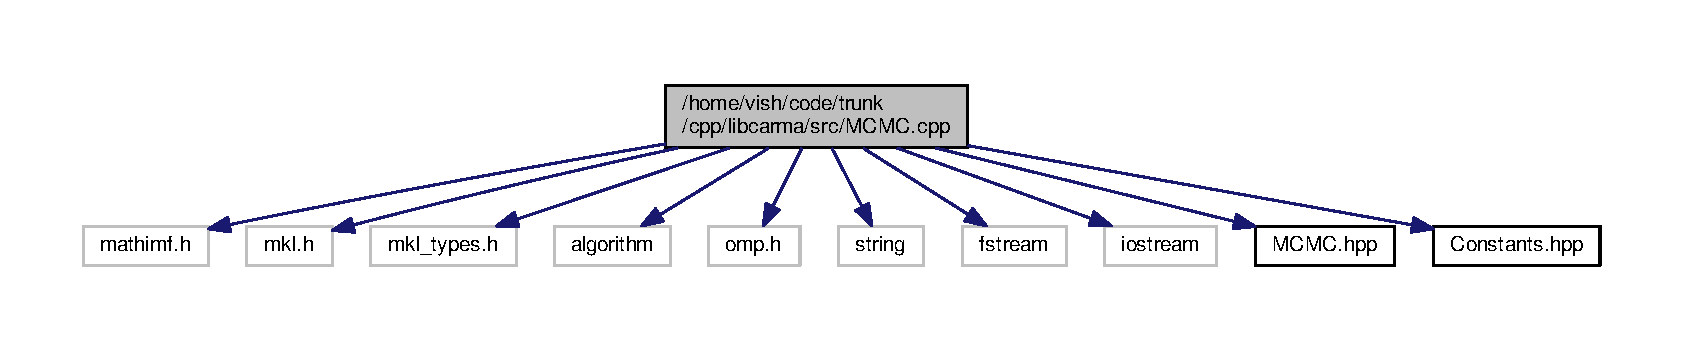
\includegraphics[width=350pt]{_m_c_m_c_8cpp__incl}
\end{center}
\end{figure}

\hypertarget{rand_8cpp}{\section{/home/vish/code/trunk/cpp/libcarma/cython/src/rand.cpp File Reference}
\label{rand_8cpp}\index{/home/vish/code/trunk/cpp/libcarma/cython/src/rand.\-cpp@{/home/vish/code/trunk/cpp/libcarma/cython/src/rand.\-cpp}}
}
{\ttfamily \#include \char`\"{}Python.\-h\char`\"{}}\\*
Include dependency graph for rand.\-cpp\-:
\subsection*{Macros}
\begin{DoxyCompactItemize}
\item 
\#define \hyperlink{rand_8cpp_ac9efdaac9411d0868b715edccca3269d}{P\-Y\-\_\-\-S\-S\-I\-Z\-E\-\_\-\-T\-\_\-\-C\-L\-E\-A\-N}
\end{DoxyCompactItemize}


\subsection{Macro Definition Documentation}
\hypertarget{rand_8cpp_ac9efdaac9411d0868b715edccca3269d}{\index{rand.\-cpp@{rand.\-cpp}!P\-Y\-\_\-\-S\-S\-I\-Z\-E\-\_\-\-T\-\_\-\-C\-L\-E\-A\-N@{P\-Y\-\_\-\-S\-S\-I\-Z\-E\-\_\-\-T\-\_\-\-C\-L\-E\-A\-N}}
\index{P\-Y\-\_\-\-S\-S\-I\-Z\-E\-\_\-\-T\-\_\-\-C\-L\-E\-A\-N@{P\-Y\-\_\-\-S\-S\-I\-Z\-E\-\_\-\-T\-\_\-\-C\-L\-E\-A\-N}!rand.cpp@{rand.\-cpp}}
\subsubsection[{P\-Y\-\_\-\-S\-S\-I\-Z\-E\-\_\-\-T\-\_\-\-C\-L\-E\-A\-N}]{\setlength{\rightskip}{0pt plus 5cm}\#define P\-Y\-\_\-\-S\-S\-I\-Z\-E\-\_\-\-T\-\_\-\-C\-L\-E\-A\-N}}\label{rand_8cpp_ac9efdaac9411d0868b715edccca3269d}


Definition at line 53 of file rand.\-cpp.


\hypertarget{rdrand_8cpp}{\section{/home/vish/code/trunk/cpp/libcarma/cython/src/rdrand.cpp File Reference}
\label{rdrand_8cpp}\index{/home/vish/code/trunk/cpp/libcarma/cython/src/rdrand.\-cpp@{/home/vish/code/trunk/cpp/libcarma/cython/src/rdrand.\-cpp}}
}
{\ttfamily \#include \char`\"{}rdrand.\-hpp\char`\"{}}\\*
{\ttfamily \#include $<$string.\-h$>$}\\*
{\ttfamily \#include $<$stdint.\-h$>$}\\*
Include dependency graph for rdrand.\-cpp\-:
\subsection*{Macros}
\begin{DoxyCompactItemize}
\item 
\#define \hyperlink{rdrand_8cpp_af7b2fee6da8e44ce8d6a0e4a5262d079}{R\-D\-R\-A\-N\-D\-\_\-\-M\-A\-S\-K}~0x40000000
\item 
\#define \hyperlink{rdrand_8cpp_ad4eba3b0ea03f397bae8792d0f0e4cd4}{R\-E\-T\-R\-Y\-\_\-\-L\-I\-M\-I\-T}~10
\end{DoxyCompactItemize}
\subsection*{Typedefs}
\begin{DoxyCompactItemize}
\item 
typedef uint32\-\_\-t \hyperlink{rdrand_8cpp_acd2b4a4f9b95333d55673ab3b5a879c6}{\-\_\-wordlen\-\_\-t}
\end{DoxyCompactItemize}
\subsection*{Functions}
\begin{DoxyCompactItemize}
\item 
int \hyperlink{rdrand_8cpp_a092ff5b5cdd0009b9a39bd9a087e5ee8}{Rd\-Rand\-\_\-cpuid} ()
\begin{DoxyCompactList}\small\item\em Queries cpuid to see if rdrand is supported. \end{DoxyCompactList}\item 
int \hyperlink{rdrand_8cpp_a53e99256bfc3ab954115658e09ff0b7c}{Rd\-Rand\-\_\-is\-Supported} ()
\begin{DoxyCompactList}\small\item\em Determines whether or not rdrand is supported by the C\-P\-U. \end{DoxyCompactList}\item 
int \hyperlink{rdrand_8cpp_ac0b6836005a9eeaa7fc22e8ec128da4c}{rdrand\-\_\-16} (uint16\-\_\-t $\ast$x, int retry)
\begin{DoxyCompactList}\small\item\em Calls rdrand for a 16-\/bit result. \end{DoxyCompactList}\item 
int \hyperlink{rdrand_8cpp_ae5322e4aa5e55c40875b980638726001}{rdrand\-\_\-32} (uint32\-\_\-t $\ast$x, int retry)
\begin{DoxyCompactList}\small\item\em Calls rdrand for a 32-\/byte result. \end{DoxyCompactList}\item 
int \hyperlink{rdrand_8cpp_a2982203449ab462050e54165e8f091db}{rdrand\-\_\-64} (uint64\-\_\-t $\ast$x, int retry)
\begin{DoxyCompactList}\small\item\em Calls rdrand for a 64-\/byte result. \end{DoxyCompactList}\item 
int \hyperlink{rdrand_8cpp_a2e933b7b559d673f1b22a64710b772f7}{rdrand\-\_\-get\-\_\-n\-\_\-64} (unsigned int n, uint64\-\_\-t $\ast$dest)
\begin{DoxyCompactList}\small\item\em Calls rdrand to obtain multiple 64-\/byte results. \end{DoxyCompactList}\item 
int \hyperlink{rdrand_8cpp_a226c1c992d91231a6d0c374b3ccb3f44}{rdrand\-\_\-get\-\_\-n\-\_\-32} (unsigned int n, uint32\-\_\-t $\ast$dest)
\begin{DoxyCompactList}\small\item\em Calls rdrand to obtain multiple 32-\/byte results. \end{DoxyCompactList}\item 
int \hyperlink{rdrand_8cpp_a1908b1f4b65c4dabc7cfdff97b488095}{rdrand\-\_\-get\-\_\-bytes} (unsigned int n, unsigned char $\ast$dest)
\begin{DoxyCompactList}\small\item\em Calls rdrand to fill a buffer of arbitrary size with random bytes. \end{DoxyCompactList}\end{DoxyCompactItemize}


\subsection{Macro Definition Documentation}
\hypertarget{rdrand_8cpp_af7b2fee6da8e44ce8d6a0e4a5262d079}{\index{rdrand.\-cpp@{rdrand.\-cpp}!R\-D\-R\-A\-N\-D\-\_\-\-M\-A\-S\-K@{R\-D\-R\-A\-N\-D\-\_\-\-M\-A\-S\-K}}
\index{R\-D\-R\-A\-N\-D\-\_\-\-M\-A\-S\-K@{R\-D\-R\-A\-N\-D\-\_\-\-M\-A\-S\-K}!rdrand.cpp@{rdrand.\-cpp}}
\subsubsection[{R\-D\-R\-A\-N\-D\-\_\-\-M\-A\-S\-K}]{\setlength{\rightskip}{0pt plus 5cm}\#define R\-D\-R\-A\-N\-D\-\_\-\-M\-A\-S\-K~0x40000000}}\label{rdrand_8cpp_af7b2fee6da8e44ce8d6a0e4a5262d079}
The bit mask used to examine the ecx register returned by cpuid. The 30th bit is set. 

Definition at line 39 of file rdrand.\-cpp.

\hypertarget{rdrand_8cpp_ad4eba3b0ea03f397bae8792d0f0e4cd4}{\index{rdrand.\-cpp@{rdrand.\-cpp}!R\-E\-T\-R\-Y\-\_\-\-L\-I\-M\-I\-T@{R\-E\-T\-R\-Y\-\_\-\-L\-I\-M\-I\-T}}
\index{R\-E\-T\-R\-Y\-\_\-\-L\-I\-M\-I\-T@{R\-E\-T\-R\-Y\-\_\-\-L\-I\-M\-I\-T}!rdrand.cpp@{rdrand.\-cpp}}
\subsubsection[{R\-E\-T\-R\-Y\-\_\-\-L\-I\-M\-I\-T}]{\setlength{\rightskip}{0pt plus 5cm}\#define R\-E\-T\-R\-Y\-\_\-\-L\-I\-M\-I\-T~10}}\label{rdrand_8cpp_ad4eba3b0ea03f397bae8792d0f0e4cd4}


Definition at line 41 of file rdrand.\-cpp.



\subsection{Typedef Documentation}
\hypertarget{rdrand_8cpp_acd2b4a4f9b95333d55673ab3b5a879c6}{\index{rdrand.\-cpp@{rdrand.\-cpp}!\-\_\-wordlen\-\_\-t@{\-\_\-wordlen\-\_\-t}}
\index{\-\_\-wordlen\-\_\-t@{\-\_\-wordlen\-\_\-t}!rdrand.cpp@{rdrand.\-cpp}}
\subsubsection[{\-\_\-wordlen\-\_\-t}]{\setlength{\rightskip}{0pt plus 5cm}typedef uint32\-\_\-t {\bf \-\_\-wordlen\-\_\-t}}}\label{rdrand_8cpp_acd2b4a4f9b95333d55673ab3b5a879c6}


Definition at line 50 of file rdrand.\-cpp.



\subsection{Function Documentation}
\hypertarget{rdrand_8cpp_ac0b6836005a9eeaa7fc22e8ec128da4c}{\index{rdrand.\-cpp@{rdrand.\-cpp}!rdrand\-\_\-16@{rdrand\-\_\-16}}
\index{rdrand\-\_\-16@{rdrand\-\_\-16}!rdrand.cpp@{rdrand.\-cpp}}
\subsubsection[{rdrand\-\_\-16}]{\setlength{\rightskip}{0pt plus 5cm}int rdrand\-\_\-16 (
\begin{DoxyParamCaption}
\item[{uint16\-\_\-t $\ast$}]{x, }
\item[{int}]{retry}
\end{DoxyParamCaption}
)}}\label{rdrand_8cpp_ac0b6836005a9eeaa7fc22e8ec128da4c}


Calls rdrand for a 16-\/bit result. 

This function calls rdrand requesting a 16-\/bit result. By default, it will perform only a single call to rdrand, returning success or failure. On success, the data is written to memory pointed to by x. If the int retry is true (non-\/zero), the function will enter a loop with count=10 until rdrand succeeds, at which point it write the random data and return success, or fails This function also ensures that rdrand is supported by the cpu or fails gracefully.


\begin{DoxyParams}{Parameters}
{\em x} & pointer to memory to store the random result \\
\hline
{\em retry} & int to determine whether or not to loop until rdrand succeeds or until 10 failed attempts\\
\hline
\end{DoxyParams}
\begin{DoxyReturn}{Returns}
whether or not the call was successful, or supported at all 
\end{DoxyReturn}


Definition at line 179 of file rdrand.\-cpp.



Here is the call graph for this function\-:


\hypertarget{rdrand_8cpp_ae5322e4aa5e55c40875b980638726001}{\index{rdrand.\-cpp@{rdrand.\-cpp}!rdrand\-\_\-32@{rdrand\-\_\-32}}
\index{rdrand\-\_\-32@{rdrand\-\_\-32}!rdrand.cpp@{rdrand.\-cpp}}
\subsubsection[{rdrand\-\_\-32}]{\setlength{\rightskip}{0pt plus 5cm}int rdrand\-\_\-32 (
\begin{DoxyParamCaption}
\item[{uint32\-\_\-t $\ast$}]{x, }
\item[{int}]{retry}
\end{DoxyParamCaption}
)}}\label{rdrand_8cpp_ae5322e4aa5e55c40875b980638726001}


Calls rdrand for a 32-\/byte result. 

This function calls rdrand requesting a 32-\/bit result. By default, it will perform only a single call to rdrand, returning success or failure. On success, the data is written to memory pointed to by x. If the int retry is true (non-\/zero), the function will enter a loop with count=10 until rdrand succeeds, at which point it write the random data and return success, or fails This function also ensures that rdrand is supported by the cpu or fails gracefully.


\begin{DoxyParams}{Parameters}
{\em x} & pointer to memory to store the random result \\
\hline
{\em retry} & int to determine whether or not to loop until rdrand succeeds or until 10 failed attempts\\
\hline
\end{DoxyParams}
\begin{DoxyReturn}{Returns}
whether or not the call was successful, or supported at all 
\end{DoxyReturn}


Definition at line 209 of file rdrand.\-cpp.



Here is the call graph for this function\-:




Here is the caller graph for this function\-:


\hypertarget{rdrand_8cpp_a2982203449ab462050e54165e8f091db}{\index{rdrand.\-cpp@{rdrand.\-cpp}!rdrand\-\_\-64@{rdrand\-\_\-64}}
\index{rdrand\-\_\-64@{rdrand\-\_\-64}!rdrand.cpp@{rdrand.\-cpp}}
\subsubsection[{rdrand\-\_\-64}]{\setlength{\rightskip}{0pt plus 5cm}int rdrand\-\_\-64 (
\begin{DoxyParamCaption}
\item[{uint64\-\_\-t $\ast$}]{x, }
\item[{int}]{retry}
\end{DoxyParamCaption}
)}}\label{rdrand_8cpp_a2982203449ab462050e54165e8f091db}


Calls rdrand for a 64-\/byte result. 

This function calls rdrand requesting a 64-\/byte result. By default, it will perform only a single call to rdrand, returning success or failure. On success, the data is written to memory pointed to by x. If the int retry is true (non-\/zero), the function will enter a loop with count=10 until rdrand succeeds, at which point it write the random data and return success, or fails This function also ensures that rdrand is supported by the cpu or fails gracefully.

Calling rdrand\-\_\-64 on a 32-\/bit system is inefficient as it makes two calls to rdrand\-\_\-32 to produce a single 64-\/bit value, using a shift to populate the high bits. The physical construction of the D\-R\-N\-G allows you to do this up to a 128-\/bit value while retaining multiplicative prediction resistance (i.\-e., don't do this to generate numbers larger than 128 bits).


\begin{DoxyParams}{Parameters}
{\em x} & pointer to memory to store the random result \\
\hline
{\em retry} & int to determine whether or not to loop until rdrand succeeds or until 10 failed attempts\\
\hline
\end{DoxyParams}
\begin{DoxyReturn}{Returns}
whether or not the call was successful, or supported at all 
\end{DoxyReturn}


Definition at line 239 of file rdrand.\-cpp.



Here is the call graph for this function\-:




Here is the caller graph for this function\-:


\hypertarget{rdrand_8cpp_a092ff5b5cdd0009b9a39bd9a087e5ee8}{\index{rdrand.\-cpp@{rdrand.\-cpp}!Rd\-Rand\-\_\-cpuid@{Rd\-Rand\-\_\-cpuid}}
\index{Rd\-Rand\-\_\-cpuid@{Rd\-Rand\-\_\-cpuid}!rdrand.cpp@{rdrand.\-cpp}}
\subsubsection[{Rd\-Rand\-\_\-cpuid}]{\setlength{\rightskip}{0pt plus 5cm}int Rd\-Rand\-\_\-cpuid (
\begin{DoxyParamCaption}
{}
\end{DoxyParamCaption}
)}}\label{rdrand_8cpp_a092ff5b5cdd0009b9a39bd9a087e5ee8}


Queries cpuid to see if rdrand is supported. 

rdrand support in a C\-P\-U is determined by examining the 30th bit of the ecx register after calling cpuid.

\begin{DoxyReturn}{Returns}
bool of whether or not rdrand is supported 
\end{DoxyReturn}


Definition at line 129 of file rdrand.\-cpp.



Here is the caller graph for this function\-:


\hypertarget{rdrand_8cpp_a1908b1f4b65c4dabc7cfdff97b488095}{\index{rdrand.\-cpp@{rdrand.\-cpp}!rdrand\-\_\-get\-\_\-bytes@{rdrand\-\_\-get\-\_\-bytes}}
\index{rdrand\-\_\-get\-\_\-bytes@{rdrand\-\_\-get\-\_\-bytes}!rdrand.cpp@{rdrand.\-cpp}}
\subsubsection[{rdrand\-\_\-get\-\_\-bytes}]{\setlength{\rightskip}{0pt plus 5cm}int rdrand\-\_\-get\-\_\-bytes (
\begin{DoxyParamCaption}
\item[{unsigned int}]{n, }
\item[{unsigned char $\ast$}]{buffer}
\end{DoxyParamCaption}
)}}\label{rdrand_8cpp_a1908b1f4b65c4dabc7cfdff97b488095}


Calls rdrand to fill a buffer of arbitrary size with random bytes. 

This function calls rdrand requesting multiple 64-\/ or 32-\/bit results to fill a buffer of arbitrary size.


\begin{DoxyParams}{Parameters}
{\em n} & size of the buffer to fill with random bytes \\
\hline
{\em buffer} & pointer to memory to store the random result\\
\hline
\end{DoxyParams}
\begin{DoxyReturn}{Returns}
whether or not the call was successful, or supported at all 
\end{DoxyReturn}


Definition at line 307 of file rdrand.\-cpp.



Here is the call graph for this function\-:


\hypertarget{rdrand_8cpp_a226c1c992d91231a6d0c374b3ccb3f44}{\index{rdrand.\-cpp@{rdrand.\-cpp}!rdrand\-\_\-get\-\_\-n\-\_\-32@{rdrand\-\_\-get\-\_\-n\-\_\-32}}
\index{rdrand\-\_\-get\-\_\-n\-\_\-32@{rdrand\-\_\-get\-\_\-n\-\_\-32}!rdrand.cpp@{rdrand.\-cpp}}
\subsubsection[{rdrand\-\_\-get\-\_\-n\-\_\-32}]{\setlength{\rightskip}{0pt plus 5cm}int rdrand\-\_\-get\-\_\-n\-\_\-32 (
\begin{DoxyParamCaption}
\item[{unsigned int}]{n, }
\item[{uint32\-\_\-t $\ast$}]{x}
\end{DoxyParamCaption}
)}}\label{rdrand_8cpp_a226c1c992d91231a6d0c374b3ccb3f44}


Calls rdrand to obtain multiple 32-\/byte results. 

This function calls rdrand requesting multiple 32-\/byte results. On success, the data is written to memory pointed to by x. This function calls rdrand\-\_\-32 and if any of those invocations fail, this function fails. It returns the same values as rdrand\-\_\-32. 

Definition at line 288 of file rdrand.\-cpp.



Here is the call graph for this function\-:




Here is the caller graph for this function\-:


\hypertarget{rdrand_8cpp_a2e933b7b559d673f1b22a64710b772f7}{\index{rdrand.\-cpp@{rdrand.\-cpp}!rdrand\-\_\-get\-\_\-n\-\_\-64@{rdrand\-\_\-get\-\_\-n\-\_\-64}}
\index{rdrand\-\_\-get\-\_\-n\-\_\-64@{rdrand\-\_\-get\-\_\-n\-\_\-64}!rdrand.cpp@{rdrand.\-cpp}}
\subsubsection[{rdrand\-\_\-get\-\_\-n\-\_\-64}]{\setlength{\rightskip}{0pt plus 5cm}int rdrand\-\_\-get\-\_\-n\-\_\-64 (
\begin{DoxyParamCaption}
\item[{unsigned int}]{n, }
\item[{uint64\-\_\-t $\ast$}]{x}
\end{DoxyParamCaption}
)}}\label{rdrand_8cpp_a2e933b7b559d673f1b22a64710b772f7}


Calls rdrand to obtain multiple 64-\/byte results. 

This function calls rdrand requesting multiple 64-\/byte results. On success, the data is written to memory pointed to by x. This function calls rdrand\-\_\-64 and if any of those invocations fail, this function fails. It returns the same values as rdrand\-\_\-64.

This function is inefficient on 32-\/bit systems. 

Definition at line 269 of file rdrand.\-cpp.



Here is the call graph for this function\-:




Here is the caller graph for this function\-:


\hypertarget{rdrand_8cpp_a53e99256bfc3ab954115658e09ff0b7c}{\index{rdrand.\-cpp@{rdrand.\-cpp}!Rd\-Rand\-\_\-is\-Supported@{Rd\-Rand\-\_\-is\-Supported}}
\index{Rd\-Rand\-\_\-is\-Supported@{Rd\-Rand\-\_\-is\-Supported}!rdrand.cpp@{rdrand.\-cpp}}
\subsubsection[{Rd\-Rand\-\_\-is\-Supported}]{\setlength{\rightskip}{0pt plus 5cm}int Rd\-Rand\-\_\-is\-Supported (
\begin{DoxyParamCaption}
{}
\end{DoxyParamCaption}
)}}\label{rdrand_8cpp_a53e99256bfc3ab954115658e09ff0b7c}


Determines whether or not rdrand is supported by the C\-P\-U. 

This function simply serves as a cache of the result provided by cpuid, since calling cpuid is so expensive. The result is stored in a static variable to save from calling cpuid on each invocation of rdrand.

\begin{DoxyReturn}{Returns}
bool/int of whether or not rdrand is supported 
\end{DoxyReturn}


Definition at line 164 of file rdrand.\-cpp.



Here is the call graph for this function\-:




Here is the caller graph for this function\-:



\hypertarget{_task_8cpp}{\section{/home/vish/code/trunk/cpp/libcarma/cython/src/\-Task.cpp File Reference}
\label{_task_8cpp}\index{/home/vish/code/trunk/cpp/libcarma/cython/src/\-Task.\-cpp@{/home/vish/code/trunk/cpp/libcarma/cython/src/\-Task.\-cpp}}
}
{\ttfamily \#include $<$mathimf.\-h$>$}\\*
{\ttfamily \#include $<$complex$>$}\\*
{\ttfamily \#include $<$mkl.\-h$>$}\\*
{\ttfamily \#include $<$mkl\-\_\-types.\-h$>$}\\*
{\ttfamily \#include $<$omp.\-h$>$}\\*
{\ttfamily \#include $<$limits$>$}\\*
{\ttfamily \#include $<$nlopt.\-hpp$>$}\\*
{\ttfamily \#include $<$stdio.\-h$>$}\\*
{\ttfamily \#include \char`\"{}C\-A\-R\-M\-A.\-hpp\char`\"{}}\\*
{\ttfamily \#include \char`\"{}M\-C\-M\-C.\-hpp\char`\"{}}\\*
{\ttfamily \#include \char`\"{}Constants.\-hpp\char`\"{}}\\*
{\ttfamily \#include \char`\"{}L\-C.\-hpp\char`\"{}}\\*
{\ttfamily \#include \char`\"{}Task.\-hpp\char`\"{}}\\*
Include dependency graph for Task.\-cpp\-:

%--- End generated contents ---

% Index
\newpage
\phantomsection
\addcontentsline{toc}{chapter}{Index}
\printindex

\end{document}
